%%%%%%%%%%%%%%%%%%%%%%%%%%%%%%%%%%%%%%%%%
% Masters/Doctoral Thesis 
% LaTeX Template
% Version 1.43 (17/5/14)
%
% This template has been downloaded from:
% http://www.LaTeXTemplates.com
%
% Original authors:
% Steven Gunn 
% http://users.ecs.soton.ac.uk/srg/softwaretools/document/templates/
% and
% Sunil Patel
% http://www.sunilpatel.co.uk/thesis-template/
%
% License:
% CC BY-NC-SA 3.0 (http://creativecommons.org/licenses/by-nc-sa/3.0/)
%
% Note:
% Make sure to edit document variables in the Thesis.cls file
%
%%%%%%%%%%%%%%%%%%%%%%%%%%%%%%%%%%%%%%%%%

%----------------------------------------------------------------------------------------
%	PACKAGES AND OTHER DOCUMENT CONFIGURATIONS
%----------------------------------------------------------------------------------------

\documentclass[11pt, oneside]{Thesis} % The default font size and one-sided printing (no margin offsets)

\graphicspath{{figures/}} % Specifies the directory where pictures are stored

\usepackage[comma, sort&compress]{natbib} % Use the natbib
% removed 'numbers' to get years
\usepackage[]{afterpage} % Use the natbib 
\usepackage[]{siunitx}
\sisetup{range-phrase=--}
\sisetup{range-units=single}
% reference package - read up on this to edit the reference style; if you want 
% text (e.g. Smith et al., 2012) for the in-text references (instead of numbers), 
% remove 'numbers'

% FIGURES - Uncomment these three lines to have figures pushed to end of 
% chapters
% \usepackage[nolists]{endfloat}
% \renewcommand{\theposttable}{\arabic{chapter}.\arabic{posttbl}}
% \renewcommand{\thepostfigure}{\arabic{chapter}.\arabic{postfig}}

\hypersetup{urlcolor=blue, colorlinks=true} % Colors hyperlinks in blue - change 
% to black if annoying
\title{\ttitle} % Defines the thesis title - don't touch this

\begin{document}

\frontmatter % Use roman page numbering style (i, ii, iii, iv...) for the pre-content pages

\setstretch{1.3} % Line spacing of 1.3

% Define the page headers using the FancyHdr package and set up for one-sided printing
\fancyhead{} % Clears all page headers and footers
\rhead{\thepage} % Sets the right side header to show the page number
\lhead{} % Clears the left side page header

\pagestyle{fancy} % Finally, use the "fancy" page style to implement the FancyHdr headers

\newcommand{\HRule}{\rule{\linewidth}{0.5mm}} % New command to make the lines in the title page

% PDF meta-data
\hypersetup{pdftitle={\ttitle}}
\hypersetup{pdfsubject=\subjectname}
\hypersetup{pdfauthor=\authornames}
\hypersetup{pdfkeywords=\keywordnames}

%----------------------------------------------------------------------------------------
%	TITLE PAGE
%----------------------------------------------------------------------------------------

\begin{titlepage}
\begin{center}

\textsc{\LARGE \univname}\\[1.5cm] % University name
\textsc{\Large Doctoral Thesis}\\[0.5cm] % Thesis type

\HRule \\[0.4cm] % Horizontal line
{\huge \bfseries \ttitle}\\[0.4cm] % Thesis title
\HRule \\[1.5cm] % Horizontal line
 
\begin{minipage}{0.4\textwidth}
\begin{flushleft} \large
\emph{Author:}\\
\authornames % Author name - remove the \href bracket to remove the link
\end{flushleft}
\end{minipage}
\begin{minipage}{0.4\textwidth}
\begin{flushright} \large
\emph{Supervisor:} \\
\supname % Supervisor name - remove the \href bracket to remove the link  
\end{flushright}
\end{minipage}\\[3cm]
 
\large \textit{A thesis submitted in fulfilment of the requirements\\ for the degree of \degreename}\\[0.3cm] % University requirement text
\textit{in the}\\[0.4cm]
\deptname\\[2cm] % Research group name and department name
 
{\large \today}\\[4cm] % Date
%\includegraphics{Logo} % University/department logo - uncomment to place it
 
\vfill
\end{center}

\end{titlepage}

%----------------------------------------------------------------------------------------
%	DECLARATION PAGE
%	Your institution may give you a different text to place here
%----------------------------------------------------------------------------------------

\Declaration{

\addtocontents{toc}{\vspace{1em}} % Add a gap in the Contents, for aesthetics

I, \authornames, declare that this thesis titled, '\ttitle' and the work presented in it are my own. I confirm that:

\begin{itemize} 
\item[\tiny{$\blacksquare$}] This work was done wholly or mainly while in candidature for a research degree at this University.
\item[\tiny{$\blacksquare$}] Where any part of this thesis has previously been submitted for a degree or any other qualification at this University or any other institution, this has been clearly stated.
\item[\tiny{$\blacksquare$}] Where I have consulted the published work of others, this is always clearly attributed.
\item[\tiny{$\blacksquare$}] Where I have quoted from the work of others, the source is always given. With the exception of such quotations, this thesis is entirely my own work.
\item[\tiny{$\blacksquare$}] I have acknowledged all main sources of help.
\item[\tiny{$\blacksquare$}] Where the thesis is based on work done by myself jointly with others, I have made clear exactly what was done by others and what I have contributed myself.\\
\end{itemize}
 
Signed:\\
\rule[1em]{25em}{0.5pt} % This prints a line for the signature
 
Date:\\
\rule[1em]{25em}{0.5pt} % This prints a line to write the date
}

\clearpage % Start a new page

%----------------------------------------------------------------------------------------
%	QUOTATION PAGE
%----------------------------------------------------------------------------------------

\pagestyle{empty} % No headers or footers for the following pages

\null\vfill % Add some space to move the quote down the page a bit

\raggedright
\textit{``I used to think correlation implied causation, then I took a 
statistics class.\\
Now I don't."}\\
\raggedleft\textit{``Sounds like the class helped"}\\
\raggedright
\textit{``Well, maybe"}

\begin{flushright}
Randall Munroe
\end{flushright}

\vfill\vfill\vfill\vfill\vfill\vfill\null % Add some space at the bottom to position the quote 

\clearpage % Start a new page

%----------------------------------------------------------------------------------------
%	ABSTRACT PAGE
%----------------------------------------------------------------------------------------

\addtotoc{Abstract} % Add the "Abstract" page entry to the Contents

\abstract{\addtocontents{toc}{\vspace{1em}} % Add a gap in the Contents, for aesthetics

In global warming scenarios, global land surface temperatures ($T_{land}$) warm 
with greater amplitude than sea surface temperatures (SSTs), leading to a 
land/sea warming contrast even in equilibrium. Similarly, the interannual 
variability of $T_{land}$ is larger than the covariant interannual SST
variability, leading to a land/sea contrast in natural variability.  This work 
investigates the land/sea contrast in natural variability based on global 
observations, coupled general circulation model simulations and idealised 
atmospheric general circulation model simulations with different SST forcings. 

The land/sea temperature contrast in interannual variability is found to exist 
in observations and models to a varying extent in global, tropical and 
extra-tropical bands. There is agreement between models and observations in the 
tropics but not the extra-tropics. Causality in the land-sea relationship is 
explored with modelling experiments forced with prescribed SSTs, where an 
amplification of the imposed SST variability is seen over land.  The 
amplification of $T_{land}$ to tropical SST anomalies is due to the enhanced 
upper level atmospheric warming that corresponds with tropical moist convection 
over oceans leading to upper level temperature variations that are larger in 
amplitude than the source SST anomalies. This mechanism is similar to that 
proposed for explaining the equilibrium global warming land/sea warming 
contrast.

The link of the $T_{land}$ to the dominant mode of tropical and global 
interannual climate variability, the El Ni{\~n}o Southern Oscillation (ENSO), is 
found to be an indirect and delayed connection. ENSO SST variability affects the 
oceans outside the tropical Pacific, which in turn leads to a further, amplified 
and delayed response of $T_{land}$.
}

\clearpage % Start a new page

%----------------------------------------------------------------------------------------
%	ACKNOWLEDGEMENTS
%----------------------------------------------------------------------------------------

\setstretch{1.3} % Reset the line-spacing to 1.3 for body text (if it has changed)

\acknowledgements{\addtocontents{toc}{\vspace{1em}} % Add a gap in the Contents, for aesthetics

The acknowledgements and the people to thank go here, don't forget to include your project advisor\ldots
}
\clearpage % Start a new page

%----------------------------------------------------------------------------------------
%	LIST OF CONTENTS/FIGURES/TABLES PAGES
%----------------------------------------------------------------------------------------

\pagestyle{fancy} % The page style headers have been "empty" all this time, now use the "fancy" headers as defined before to bring them back

\lhead{\emph{Contents}} % Set the left side page header to "Contents"
\tableofcontents % Write out the Table of Contents

\lhead{\emph{List of Figures}} % Set the left side page header to "List of Figures"
\listoffigures % Write out the List of Figures

\lhead{\emph{List of Tables}} % Set the left side page header to "List of Tables"
\listoftables % Write out the List of Tables

%----------------------------------------------------------------------------------------
%	ABBREVIATIONS
%----------------------------------------------------------------------------------------

\clearpage % Start a new page

\setstretch{1.5} % Set the line spacing to 1.5, this makes the following tables easier to read

\lhead{\emph{Abbreviations}} % Set the left side page header to "Abbreviations"
\listofsymbols{ll} % Include a list of Abbreviations (a table of two columns)
{
\textbf{SST} & \textbf{S}ea \textbf{S}urface \textbf{T}emperature \\
\textbf{LCL} & \textbf{L}ifting \textbf{C}ondesation \textbf{L}evel \\
\textbf{WTG} & \textbf{W}eak \textbf{T}emperature \textbf{G}radient \\
	\textbf{PFixT} & \textbf{P}ressure (above which to) \textbf{F}ix the 
	\textbf{T}emperature (when using WTG Mode) \\
\textbf{ENSO} & \textbf{E}l \textbf{N}i{\~n}o-\textbf{S}outhern 
	\textbf{O}scillation \\
\textbf{CGCM} & \textbf{C}oupled \textbf{G}eneral \textbf{C}irculation 
	\textbf{M}odel \\
\textbf{AGCM} & \textbf{A}tmosphere-only \textbf{G}eneral \textbf{C}irculation 
	\textbf{M}odel \\
\textbf{CMIP} & \textbf{C}oupled \textbf{M}odel \textbf{I}nter-comparison 
	\textbf{P}roject \\
\textbf{AMIP} & \textbf{A}tmosphere-only \textbf{M}odel 
	\textbf{I}nter-comparison \textbf{P}roject \\
\textbf{ECMWF} & \textbf{E}uropean \textbf{C}enter for \textbf{M}edium Range 
	\textbf{W}eather  \textbf{F}oreasts\\
\textbf{GREB} & \textbf{G}lobally \textbf{R}esolved \textbf{E}nergy 
	\textbf{B}alance Model \\
	\textbf{ACCESS} &  \textbf{A}ustralian \textbf{C}ommunity \textbf{C}limate 
	and \textbf{E}arth \textbf{S}ystem \textbf{S}imulator \\
%\textbf{Acronym} & \textbf{W}hat (it) \textbf{S}tands \textbf{F}or \\
}

%----------------------------------------------------------------------------------------
%	PHYSICAL CONSTANTS/OTHER DEFINITIONS
%----------------------------------------------------------------------------------------

\clearpage % Start a new page

\lhead{\emph{Physical Constants}} % Set the left side page header to "Physical Constants"

\listofconstants{lrcl} % Include a list of Physical Constants (a four column table)
{
Speed of Light & $c$ & $=$ & $2.997\ 924\ 58\times10^{8}\ \mbox{ms}^{-\mbox{s}}$ (exact)\\
% Constant Name & Symbol & = & Constant Value (with units) \\
}

%----------------------------------------------------------------------------------------
%	SYMBOLS
%----------------------------------------------------------------------------------------

\clearpage % Start a new page

\lhead{\emph{Symbols}} % Set the left side page header to "Symbols"

\listofnomenclature{lll} % Include a list of Symbols (a three column table)
{
	$T_{land}$ & Land Surface Temperature & K \\
	$T_{ocean}$ & Ocean Surface Temperature & K \\
	$T_{tropo}$ & Tropospheric Temperature & K \\
	$R_{l/o}$ & Land/Ocean Contrast (Regression coeff of) & K/K \\
	$\theta$ & Potential Temperature & K \\
	$\Gamma_m^*$ & Saturated Moist Adiabatic Lapse Rate & K/km \\
% Symbol & Name & Unit \\

& & \\ % Gap to separate the Roman symbols from the Greek

$\omega$ & angular frequency & rads$^{-1}$ \\
% Symbol & Name & Unit \\
}

%----------------------------------------------------------------------------------------
%	DEDICATION
%----------------------------------------------------------------------------------------

\setstretch{1.3} % Return the line spacing back to 1.3

\pagestyle{empty} % Page style needs to be empty for this page

\dedicatory{For/Dedicated to/To my\ldots} % Dedication text

\addtocontents{toc}{\vspace{2em}} % Add a gap in the Contents, for aesthetics

%----------------------------------------------------------------------------------------
%	THESIS CONTENT - CHAPTERS
%----------------------------------------------------------------------------------------

\mainmatter % Begin numeric (1,2,3...) page numbering

\pagestyle{fancy} % Return the page headers back to the "fancy" style

% Include the chapters of the thesis as separate files from the Chapters folder
% Uncomment the lines as you write the chapters

% FIGURES - Uncomment these 20 lines to push figures to end of chapter
% \chapter{Introduction} % Main chapter title

\label{introduction} % Change X to a consecutive number; for referencing this 
% chapter elsewhere, use \ref{ChapterX}

\lhead{Chapter 1. \emph{Introduction}} % Change X to a consecutive number; this 
% is for the header on each page - perhaps a shortened title

%----------------------------------------------------------------------------------------
%	SECTION 1
%----------------------------------------------------------------------------------------

\section{Motivation}

When looking at a timeseries of annual global land surface ($T_{land}$) and sea 
surface temperatures (SST) there are two features which stand out; the two 
timeseries are largely covariant, and the land has greater variance than the 
ocean timeseries.  We define this increased variability of land surface relative 
to oceans as the interannual land/ocean thermal contrast. In a similar manner, 
for a transient climate the global $T_{land}$ warms with greater amplitude than 
the SST, leading to a global warming land/sea thermal contrast. In this study we 
will investigate the processes responsible for the interannual land/ocean 
contrast and test whether the processes that control the warming contrast are 
relevant for the positive and negative anomalies of natural variability.

\section{Land/Ocean Warming in Global Warming}

For a global warming scenario the ratio of land to sea warming tends to a value 
of around 1.5  (\citealt{Sutton2007}, \citealt{Lambert2007}, 
\citealt{Compo2008}, \citealt{Dommenget2009}). Previous studies have shown the 
land/sea warming contrast is not simply due to the larger heat capacity of the 
ocean when compared to land, but is a result of the dynamics of the climate 
system.  \citet{Sutton2007} described an energy balance argument; assuming the 
anomalous downward surface energy flux is equal over land and ocean 
\citep{Huntingford2000} the land/sea warming contrast is caused by the 
difference in the partitioning of the upward energy flux into sensible and 
latent heat.  \citet*{Lambert2007} proposed that the stability of land/sea 
contrast over annual, 5 year and longer timescales is maintained by a land to 
ocean heat flux where the ability of the ocean to absorb the extra heat leads to 
a damping of $T_{land}$ variability. In this scenario the value of the land/sea 
contrast depends on the ratio of the land and sea climate sensitivity parameters 
and ocean heat uptake. This can be related to the results of \citet{Sutton2007};
on timescales where the land and ocean heat uptake is sufficiently small the 
land to ocean heat transport can be ignored and the value of the land/ocean 
contrast depends only on the climate sensitivity parameters, and these 
parameters are controlled by the surface energy balance.  However, as stated by 
\citet{Byrne2013a} the energy balance argument does not give a sufficient 
quantitative value of land warming, and both theories neglect the ability of 
SSTs to influence $T_{land}$.  \citet{Joshi2008} proposed a conceptual model to 
explain how the SSTs can force $T_{land}$ and which leads to a land/sea warming 
contrast above unity.  There is a level in the atmosphere above which there is 
no significant land/sea contrast and thermal anomalies are transported 
efficiently around the globe. The lapse rate below that level is affected by 
temperature and moisture. The lower relative humidty over land results in 
steeper lapse rates that cause land temperatures to reach an equilibrium warmer 
than the oceans. In addition, the transport of moisture over land occurs at 
levels much colder than the surface which restricts moisture supply over land, 
hence increased warming does not lead to increased evaporation, further 
enhancing warming. The lapse rate theory was extended by \citet{Byrne2013a}; 
where \citet{Joshi2008} assumed that the land/ocean contrast due to 
\textit{changes} in temperature disappeared at a certain level, 
\citet{Byrne2013a} make the further assumption that the absolute temperatures 
above land and ocean converge. Secondly they assume that lapse rates are moist 
adiabatic above the lifting condensation level (LCL) and dry adiabatic below the 
LCL. The land and ocean lapse rates then differ due to the height of the LCL, 
which is higher over land due to reduced moisture availability. The first 
assumption relies on the fact that the tropical troposphere is unable to 
maintain strong temperature gradients in the tropics to homogenise tropospheric 
temperatures (this is further discussed in section \ref{intro:wtg}), and for the 
second convection must be sufficient to maintain a moist adiabatic lapse rate, 
hence their theory is most appropriate in the tropics.

The significantly different surface properties, as well as the atmospherically 
induced balance, between land and ocean are important factors in the land/ocean 
warming contrast, but there is also an assymetry in the forcing between land and 
ocean.  \citet{Compo2008} find a strong oceanic influence to recent continental 
warming and suggest increased downward longwave radiation due to 
hydrodynamic-radiative teleconnections as a mechanism.  \citet{Dommenget2009} 
demonstrates the ability of oceans to cause a land/sea contrast on interannual 
and longer time scales.  The disproportionate forcing of land temperatures by 
the ocean is due in part to the asymmetry in area but also due to atmospheric 
water vapour feedbacks.  Modelling studies suggest that up to 86\% of historic 
anthropogenically forced change in $T_{land}$ is a response to SST changes and 
14\% is due to local forcings. \citet{Dommenget2009} suggest that on global 
scales these mechanisms are also present in the warming and cooling of 
interannual variability, as shown in detrended model runs forced only with 
historic SSTs that exhibit greater variability of global $T_{land}$ than the 
input SSTs.

Thus the land/sea warming contrast is a natural phenomena that also applies to 
internal interannual to decadal climate variability.  When we think of the 
land/sea contrast in natural variability we can recognise a number of 
differences relative to that seen in global warming: Firstly, global warming is 
mostly a coherent warming on a global scale with a time evolution that is only 
going upwards for the relevent timescales, for example \citet{Compo2008} in 
figure 1b show that the pattern of observed surface air temperature change, 
calculated as the 1991--2006 average minus the 1961--1990 average, is largely 
homogeneous across the globe. In natural climate variability we have 
inhomogeneous warming and cooling patterns, some of them are regional others are 
more global, some of them have coherent warming and cooling (e.g.  multi-pole 
structures) at the same time, some of them are closer to the land and some are 
over tropical warm ocean regions and others are over the colder extra-tropical 
oceans. The El Ni{\~n}o-Southern oscillation is one such mode of variability 
which is associated with regional warming and cooling \citep{Halpert1992}. When 
we analyse the land/sea contrast in natural climate variability we have to take 
these structures into account.

\section{Tropical Interannual Variability and ENSO}

For globally averaged $T_{land}$ and SSTs spatial scales and time scales of 
interannual variability, the El Ni{\~n}o-Southern Oscillation (ENSO) and its 
teleconnections are the leading source of variability, so it's dynamics are 
likely to play an important role in the interannual land/sea contrast.  ENSO has 
a direct effect on tropical surface and tropospheric temperatures and a 
measureable influence on global average tempereratures (REF). \citet{Klein1999} 
discuss the concept of an atmospheric bridge as a method of communicating 
temperature anomalies from the equatorial Pacific to the remote tropical oceans 
(i.e. oceans outside the Pacific).  Similarly, \citet{Chiang2002} discuss a 
mechanism for warming of remote tropical oceans during El Ni{\~n}o conditions.  
The tropical tropospheric temperature ($T_{tropos}$) increases during El 
Ni{\~n}o, and is largely uniform across the tropical strip, 20S-20N. They find 
the surface temperature responds to the tropospheric forcing with a magnitude 
relative to the mixed layer depth, and the communication of the tropospheric 
temperature is via moist convective processes. \citet{Chiang2002} attributed the 
amplified response over land to the smaller thermal inertia and reduced cooling 
due to evaporation.  \citet{Chiang2005} use model simulations of the 1997-98 El 
Ni{\~n}o to study the tropospheric temperature mechanism for tropical ENSO 
teleconnections.  They found an almost instantaneous response of $T_{land}$ to  
El Ni{\~n}o and an ocean response with a 2-3 month lag with the ratio between 
$T_{tropos}$ and the surface warming signal was 1:1 for land and 1:0.3 for 
oceans. They were interested in the uniformity of remote ocean SST response to a 
tropospheric temperature heating when the surface fluxes exhibit large 
variability, and they found latent heat flux through the boundary layer and 
clear-sky longwave radiation regulate the surface response. No specific 
mechanism was proposed for land warming, although the higher ratio of warming 
was attributed to differing heat capacities of ocean and land. In addition the 
moist static energy was found to increase more than in the boundary layer than 
the troposphere, which is not the expected result from quasi-equilibrium theory 
(e.g. \citet{Brown1997}).  Their findings support the mechanism over oceans 
described by \citet{Chiang2002} as holding true on the larger scale they were 
investigating. 

\subsubsection{The Weak Temperature Gradient approximation}\label{intro:wtg}
The processes of the atmospheric bridge responsible for the El Ni{\~n}o 
teleconnections are similar in nature to the processes of the land/sea contrast 
as discussed in \citet{Joshi2008}, suggesting that the similar principles may be 
active. One aspect of the \citet{Joshi2008} lapse rate theory is that 
temperature anomalies are transported efficiently in the upper troposphere and 
it is well known that the tropical troposphere is unable to maintain strong 
temperature gradients.  Near the equator the small Coriolis parameter results in 
fast geostrophic adjustments by gravity waves and Kelvin waves that remove 
horizontal temperature gradients.  In the extra-tropics the quasi-geostrophic 
approximation gives us a simplified dynamical model, based on the balance of the 
pressure gradient force and rotation.  The WTG approximation is analagous and 
uses the small horizontal temperature and pressure gradients as a constraint on 
the large-scale flow and diabatic processes. The temperature equation can be 
simplified to give a balance between diabatic heating and vertical advection 
\citep{Sobel2001}. The usefulness of the WTG approximation doesn't quite match 
that of quasi-geostrophy due to the importance in the tropics of deep 
convection, which has it's own parameterization difficulties, but the WTG 
approximation allows for the parameterization of large-scale dynamics.  
\citet{Lintner2005}  investigated the applicability of the WTG approximation to 
the tropical response to ENSO with mixed results; tropospheric temperature 
perturbations were modelled realistically but there were errors in the 
precipitation response. Overall they concluded that errors in the rainfall 
response may indicate that an El Ni{\~n}o response is a poor proxy for large 
scale global warming but that the WTG approximation suitable for a low-order 
tropical response to a warming perturbation.


\section{Thesis outline}

The study presented here discusses the large-scale land/sea contrast in natural 
variability, focusing on interannual timescales. We will analyse the 
characteristics of the large-scale land/sea contrast variability in observations 
and Couple General Circulation Models (CGCMs) from the CMIP5 data base. The role 
of the SST in forcing the land variability will be analysed in Atmospheric 
General Circulation Models (AGCMs) forced with observed SSTs and in a series of 
sensitivity experiments with an AGCM coupled to a slab ocean model or with fixed 
SST boundary conditions forced with different idealised SST forcings, and our 
analysis will discuss the differences between tropical and extra-tropical 
regions. Simplified one and two dimensional models are used to further elucidate 
the tropospheric forcing of land surface and test how land surface 
characteristics affect the response. Finally the Globally Resolved Energy 
Balance model (GREB, \citet{Dommenget2011}) is used to quantify the contribution 
of different factors to regional land temperatures.

In this thesis, the data and model simulations are described in chapter 
\ref{methods}.  Chapter \ref{evidence} will discuss the evidence for the 
land/sea contrast larger than unity in natural variability in observations and 
model simulations. This analysis will also explore some of the regional 
differences in the ocean to land connection. In section \ref{mechanisms} we 
explore the mechanisms controlling the land/sea contrast with a series of 
sensitivity experiments that explore the role of the SST forcing, the 
differences between tropical and extra-tropical regions and that highlight the 
role on El Ni{\~n}o forcing and illustrate how the SST forcing is amplified over 
land to result into a land/sea contrast larger than unity. In the final chapter 
the study will be closed with a summary and discussion.


% \processdelayedfloats
% \setcounter{postfig}{0}
% \setcounter{posttbl}{0}
% \chapter{Data and Methods} % Main chapter title

\label{methods} % Change X to a consecutive number; for referencing this chapter 
% elsewhere, use \ref{ChapterX}

\lhead{Chapter 2. \emph{Data and Methods}} % Change X to a consecutive number; 
% this is for the header on each page - perhaps a shortened title

In this chapter we discuss the observational and model data, the models and the 
experiments conducted with them, and some of the statistical methods applied to 
the data.

%----------------------------------------------------------------------------------------
%	DATA
%----------------------------------------------------------------------------------------

\section{Data}

This section will outline the data used for this project, including processing 
performed, a discussion of uncertainties for each data set and any inherent 
limitations.

\subsection{Observational Data}

Three data products from the UK Met Office Hadley centre and the University of 
East Anglia Climatic Research Unit were used as surface temperatures 
observations; Climatic Research Unit land Temperature data set, version 
4 (CRUTEM4) \citep{Brohan2006}, the Hadley Centre SST data set,
version 2 (HadSST2) \citep{Rayner2006} and the Hadley Centre global sea ice and 
and SST, version 1 (HadISST) (ref).

HadSST2 is global gridded SST dataset based on observations, with the data 
coverage decreasing with time. Prior to 1950 data coverage is too sparse to 
allow strong statistical conclusions \citep{Dommenget2009}, and measuring the 
land/sea interactions by comparison with CRUTEM4 can lead to errors. This 
dataset, along with CRUTEM4, was used for observations as it was considered the 
truest representation, as there is no interpolation or processing done on the 
data; other than that to correct inconsistencies. (Data coverage discussion?)

CRUTEM4 is a global gridded land temperature dataset based on observations.  
Regarding the data coverage; there are large areas without data in the tropics, 
particularly in tropical Africa and Amazonian South America. Global climate 
model experiments show that these areas may be important in terms of the land 
response to tropical SST perturbations, as such the effect of this missing data 
is investigated further in Chapter \ref{evidence} by masking the model results 
to simulate the data coverage of the observations and testing the robustness of 
the statistics used to measure the land/sea contrast. It is found the data 
coverage issues may effect the magnitude of some results but not the 
conclusions.

HadISST1 is a global gridded SST dataset based on observations, and interpolated 
in regions without data. It uses the same sources as HadSST2 but as missing data 
points are interpolated there is no decreases in coverage with time. The 
increased amount of interpolation means there is no increase in information so 
the dataset is no more useful than HadSST2 when comparing to land temperatures.  
Instead, the HadISST1 data is used as the input for model runs. The data prior 
to 1950 is still used for AMIP-type experiments (see \ref{methods:amip}) because 
even though it is unsuitable for comparing the land and ocean timeseries	it 
is suitable as a representation of realistic SST variability. For the AMIP runs 
we want to see how the land surface responds to SST variability and the 
interpolated SST data is suitable for this.

All observational data was linearly detrended, as linear trends strongly 
influence correlations and would lead to spurious results. However variability 
on decadal timescales was not removed. The use of highpass filters on the data, 
which could have the effect of removing decadal length oscillations, lead to 
unrealistic results, and it was decided that simple linear detrend would be 
sufficient to remove the long-term variability most affecting any correlations 
and regressions with the least amount of processing.

\paragraph{Microwave Sounding Unit}
\begin{itemize}
	\item Description, references
	\item Temporal, areal coverage
	\item Known issues.
	\item Reason for use, relationship to l/o contrast
\end{itemize}


\subsection{Reanalysis Data}

The NCEP-Reanalysis dataset uses a forecast model (ref, details) that 
assimilates past observational data as boundary conditions. The result is a high 
spatial and temporal resolution gridded dataset of surface and tropospheric 
variables, as close to observations as possible.  Only satellite data is used 
which mean the length is limited to satellite era, post 1979. The NCEP data was 
Used in initial investigations as alternative to Hadley Centre observations.

\subsection{Coupled Model Data}

For the analysis of CGCMs we used all available pre-industrial control runs from 
the CMIP5 datasets \citep{Taylor2012}, see Table \ref{tab:cmip5} for the full 
list. The pre-industrial control runs, which lack any anthropogenic or natural 
radiative forcings (i.e. no changes in $CO_2$, volcanoes, etc)  were chosen in 
order to study the unforced internal variability. 100 years from each of the 35 
models was used, and anomalies were defined seperately for each model relative 
to its climatology. The multi-model mean of the CMIP5 data was calculated using 
the anomalous (relative to each model’s climatology) timeseries from each model, 
these were combined end-to-end to generate a 3500 year timeseries. 

\begin{center}
	\begin{table}[h]
	\caption{CMIP5 models used in this study. 100 years of the piControl run was 
	used from each model.}
		\label{tab:cmip5}
		\tiny
	\begin{tabular}{ l  l  l  l l}
		Originating Group(s) & Country & Model \\ \hline
		CSIRO and BOM & Australia & ACCESS1.0 \\
Beijing Climate Center, China Meteorological Administration & China & BCC-CSM1.1 
		 \\
Beijing Climate Center, China Meteorological Administration & China & 
		BCC-CSM1.1-m \\
		GCESS, Beijing National University & China & BNU-ESM \\
National Center for Atmospheric Research & USA & CCSM4 \\
		National Center for Atmospheric Research  & USA & CESM1-BGC  \\
		National Center for Atmospheric Research  & USA & CESM1-CAM5  \\
		National Center for Atmospheric Research  & USA & CESM1-FASTCHEM \\
		National Center for Atmospheric Research  & USA & CESM1-WACCM  \\
		Centro Euro-Mediterraneo per i Cambiamenti & Italy & CMCC-CM \\
		Centro Euro-Mediterraneo per i Cambiamenti & Italy & CMCC-CMS \\
		CSIRO and QCCCE & Australia & CSIRO-Mk3-6-0 \\
Meteo-France/Centre National de Recherches Meteorologiques & France & CNRM-CM5 
		\\
Canadian Centre for Climate Modelling and Analysis & Canada & CanESM2 \\
		Institute of Atmospheric Physics and Chinese Academy of Sciences & China & 
		FGOALS-g2 \\
		Institute of Atmospheric Physics and Chinese Academy of Sciences & China & 
		FGOALS-s2 \\
		The First Institution of Oceanography & China & FIO-ESM \\

Geophysical Fluid Dynamics Laboratory & USA & GFDL-CM3 \\
Geophysical Fluid Dynamics Laboratory & USA & GFDL-ESM2G \\
Geophysical Fluid Dynamics Laboratory & USA & GFDL-ESM2M \\
NASA / Goddard Institute for Space Studies & USA & GISS-E2-H \\
NASA / Goddard Institute for Space Studies & USA & GISS-E2-R \\
Hadley Centre for Climate Prediction and Research/Met Office & UK & HadCM3 \\
Hadley Centre for Climate Prediction and Research/Met Office & UK & HadGEM2-CC 
 \\
Hadley Centre for Climate Prediction and Research/Met Office & UK & HadGEM2-ES 
 \\
Institute for Numerical Mathematics & Russia & INM-CM4 \\
Institut Pierre Simon Laplace & France & IPSL-CM5A-LR \\
Institut Pierre Simon Laplace & France & IPSL-CM5A-MR \\
Institut Pierre Simon Laplace & France & IPSL-CM5B-LR \\
		Atmosphere and Ocean Research Institute (AORI),    & Japan & MIROC5 \\
		\	National Institute for Environmental Studies (NIES) and  &&& \\
		\	Japan Agency for Marine-Earth Science and Technology (JAMSTEC) && & \\
AORI, NIES and JAMSTEC		& Japan & MIROC-ESM \\
Max Planck Institute for Meteorology & Germany & MPI-ESM-LR \\
Max Planck Institute for Meteorology & Germany & MPI-ESM-P \\
Max Planck Institute for Meteorology & Germany & MPI-ESM-MR \\
Meteorological Research Institute & Japan & MRI-CGCM3 \\
Norwegian Climate Centre & Norway & NorESM1-M \\
Norwegian Climate Centre & Norway & NorESM1-ME \\
	\end{tabular}
	\end{table}
\end{center}


%----------------------------------------------------------------------------------------
%	MODEL EXPERIMENTS
%----------------------------------------------------------------------------------------

\section{Model Experiments}

This section will describe the models that were used, and the core experiments 
performed with each model.


\subsection{ACCESS Model}

Sensitivity experiments were performed with the UK Meteorological Office Unified 
Model AGCM with HadGEM2 atmospheric physics (\citet{Davies2005}; 
\citet{Martin2010}; \citet{Bellouin2011}) at an atmospheric resolution of N48 
($3.75^{\circ} \times 2.5^{\circ}$). The model was either forced with prescribed 
SSTs or contained a slab ocean (the slab ocean is described in section 
\ref{methods:pacemaker}).

Three primary types of experiments were conducted: AMIP-type; sensitivity to 
mean SST increases or decreases; and El Ni{\~n}o pattern forcing experiments, 
see Table \ref{tab:senseexp} for full details. The latter El Ni{\~n}o forcing 
experiment is similar to a `pacemaker' experiment, as described by 
~\citealt{Alexander1992}, ~\citealt{Alexander1992a}, ~\citealt{Lau2000} and 
~\citealt{Lu2011}. 

\begin{center}
	\begin{table}[h]
		\caption{Idealised model simulations discussed in this study. Atmospheric 
		component was HadGEM2 at N48 resolution.}
		\label{tab:senseexp}
		\scriptsize
	\begin{tabular}{ l  l  l  l l}
		\textit{Name}		&  \textit{Ocean} & \textit{Time} &\textit{ Notes }\\ \hline
	AMIP-global &    HadISST & 1870-2012 &  \\
	AMIP-tropics	   & Tropics: HadISST & 1870-2012 & Climatological SSTs with \\
		&Extra-tropics: FIXSST&& anomalies applied in tropics \\
	AMIP-extra-tropics     & Extra-tropics: HadISST & 1870-2012 & 
		Climatological SSTs with \\
		& Tropics: FIXSST && anomalies applied in extra-tropics\\
		FIXSST    & Climatology & 100 years & Climatological SSTs based  \\
								  &&& on HadISST 1950-2013 \\
		+1K Global    & FIXSST,  & 100 years & Climatology with \\
												 & +1K && +1K added to global oceans \\
		+1K Tropics     & FIXSST, & 100 years & Climatology with \\
												 & +1K in Tropics && +1K added to 
		tropical oceans \\
		+1K Extra-tropics	   & FIXSST & 100 years &Climatology with \\
											& +1K in Extra-tropics && +1K added to 
		extra-tropical oceans \\
	Slab 	   & 50m mixed layer ocean & 100 years & \\
	ENSO-FIXSST    &  FIXSST, & 100 years & Climatology with \\
											& El Ni{\~n}o pattern && oscillating 
		pattern in tropical Pacific\\
	ENSO-slab    & Slab,  & 100 years & 50m mixed layer ocean with \\
											& El Ni{\~n}o pattern && oscillating 
		pattern in tropical Pacific\\
	\hline
	\end{tabular}
	\end{table}
\end{center}


\subsubsection{AMIP-Type experiments}\label{methods:amip}
AMIP (Atmosphere-only Model Inter-comparison Project, (ref)), much like CMIP, is 
a project to compare results from many modelling centres, except instead of 
coupled ocean-atmosphere models the models are forced with observational SSTs.  
Therefore an we consider an AMIP-type experiment one where a model is forced 
with observational, or similar to observational SSTs. There are a few benefits 
to this setup; it allows us to test the effect of a range of SST anomalies on 
continental temperatures, it is computationally much cheaper than a coupled run 
and doesn't require long spin up times, and the contained boundary conditions 
stabilise the model and prevent drift. The key limitation of AMIP runs is the 
loss of atmosphere to ocean feedbacks which are potentially important for the 
eveolution of both systems. This downside is partially addressed with the use of 
a mixed-layer slab ocean, discussed in section \ref{methods:pacemaker}.

The AMIP type runs used HadISST from 1870 to 2010. While it was determined that 
HadSST2 data was only suitable from 1950 for calculating statistics relating to 
the observational value of the land/sea contrast, the HadISST data was used from 
1870. The reason is that the HadISST SSTs were primarily used as a 
representation of realistic interannual variability with which to force the 
atmospheric model.  In the AMIP runs the SST and $T_{land}$ are consistent 
because $T_{land}$ responds to the prescribed SST.  Whether or not these were 
the true SST values in the real world is not important in the context of this 
study.  We use the early SST values from HadISST to generate realistic SST 
variability; thus we can use the earlier period to get more statistics. In the 
statistical analysis of observed SST verse land the errors in the observed SST 
do matter as they no longer co-vary with the land, so we cannot use the early 
SST and $T_{land}$ values.

\subsubsection{Half-AMIP/Half-1K experiments}
Simulations forced with idealised SST patterns used a 12 month climatology of 
the HadISST data from 1950-2010 as the reference control climate. The division 
between tropics and extra-tropics for these experiments was chosen to be 
$28^{\circ}$N/S, with the tropical forcing applied to the oceans in the zonal 
band bordered by $28^{\circ}$N/S, and the extra-tropical forcing applied from 
$28^{\circ}$N/S to the poles. For the model resolution used this most closely 
divides the oceans in half by area, with slightly more area in the 
extra-tropics.

\subsubsection{Pacemaker experiment}\label{methods:pacemaker}
For the El Ni{\~n}o pattern forcing experiments a canonical El Ni{\~n}o pattern 
was generated using HadISST monthly mean data from a linear regression between 
NINO3 and SSTs, as shown in Figure 1. This pattern was imposed in the tropical 
Pacific between $30^{\circ}$N/S and $155^{\circ}$E to the eastern boundary of 
the Pacific, on to monthly climatological SSTs (i.e. a repeating 12 month 
seasonal cycle).  The values of the anomaly was based on the regression values, 
with a maximum temperature anomaly of 1.41K.  The pattern was oscillated with a 
period of 4 years, peaking in January.  Outside of the tropical Pacific there 
were two scenarios; fixed SSTs using the HadISST 1950-2010 climatology, and the 
slab ocean.  

The slab ocean is essentially a series of 1D ocean columns and assumes a 
constant mixed layer depth of 50 metres. It is forced by flux correction terms 
to have on average the HadISST 1950--2010 SST climatology \citep{Wang2014}. A 
constant mixed layer was chosen in part for simplicity as this model setup is 
intended to be of intermediate complexity, between a simple prescribed SST run 
and a fully coupled dynamic ocean. We use a slab ocean as simple way of 
modelling SST variability, and while we would expect that the response time of 
the remote oceans to an external forcing would scale with mixed layer depth 
(\citealt{Su2005a}, \citealt{Lintner2007}), the constant 50 metre assumption 
gives a first order but realistic response.  


\subsection{One and Two-Dimensional Radiative-Convective Model}
Simplified atmospheric models have long been used to elucidate the important 
mechanisms of otherwise complicated problems (references?). To understand the 
relationship between SSTs, tropospheric temperatures and $T_{land}$ response we 
used a radiative-convective column model. A radiative-convective model is one 
where the atmospheric heating by convection is balanced with radiative cooling 
(ref Manabe, Wetherald 1967 etc) [extra details?] and have been used in a myriad 
of studies, such as the equilibrium response to $CO_2$ (ref) and solar forcings 
(ref) and climate sensitivity (ref), the organisation of deep convection (ref) 
and the atmospheric sctuctural response to SSTs and boundary layer humidity 
(hamish and adam, ref).  There have been studies using RCE over simple land 
surfaces (ref) and more recently with more realistic land representations 
\citep{Rochetin2014}.

\subsubsection{Model details}
We utilised the Massachusetts Institute of Technology (MIT) RCE model. First 
described by \citet{Renno1994} and updated in \citet{Bony2001}.  The convection 
scheme was first described in \citet{Emanuel1991} and improved in 
\citet{Emanuel1999}. The radiative transfer scheme is from the European Center 
for Medium Range Weather Forecast (ECMWF) operational model, and is split into a 
shortwave scheme as described in \citet{Fouquart1980} and the longwave scheme 
from \citet{Morcrete1991a}. The fractional cloud scheme of \citet{Bony2001} is 
coupled to the convection scheme and also controls the interaction of clouds and 
radiation. The boundary layer is modeled with a dry adiabatic adjustment to all 
variables. Surface fluxes are calculated with bulk aerodynamic formulas using a 
specified wind speed.  The surface can be modelled as prescribed SSTs, a mixed 
layer ocean or a simple land surface, the latter by specifying the evaporative 
fraction and a shallow mixed layer depth. The model geometry can be set as a 
single column (1D) or as a two dimensional (2D) model in a zonal or meridional 
directions. The model can also be run in Weak Temperature Gradient mode (WTG 
mode) as described in \citet{Sobel200}. For this setup, which relys on the WTG 
approximation as discussed in section \ref{intro:wtg}, the free tropospheric 
temperature profile is specified and remains fixed, allowing the vertical 
velocity and, hence precipation to be prognostic variables.

\subsubsection{Experiments}
The low computing power required to run a simple model allows for many and 
varied experiments, as well as efficient parameter testing. There were three key 
groups of experiments performed with the MIT model; 1D prescribed SST-WTG 
experiment; 2D prescribed SST land-ocean experiment; and 2D $CO_2$ forced 
land-ocean experiment.

\subsubsection{1D SST-WTG experiment}
The 1D SST-WTG experiments consisted of two key parts; initially the model was 
run without invocation of the WTG mode and a range of temperature profiles were 
generated by varying prescribed SSTs, then these generated free tropospheric 
temperature profiles were imposed above a responsive land surface using the WTG 
mode. 

\subsubsection{2D prescribed SST land-ocean experiment}
For these experiments the model was aligned zonally or meridionally with various 
numbers of land and ocean columns, the simplest being two columns; one land, one 
ocean. These runs were forced by varying the SSTs around a mean value suitable 
for the chosen latitude.

\subsubsection{2D $CO_2$ forced land-ocean experiment}
The geometry of these experiments were similar to the 2D prescribed SST 
experiments, but instead of forcing with SST changes it was forced through 
changes in $CO_2$. Both the land and ocean columns able to respond to the 
forcing. As this study primarily deals with natural variability a $CO_2$ forced 
experiment may seem unusual but it was useful as it allowed us to test our 
assumptions about comparisons between global warming land/ocean thermal 
contrast, and an understanding of the sensitivity of the modelled land and ocean 
surfaces to an external forcing puts the other results in context.


\begin{itemize}
	\item Parameter options; land surface, model levels, interactive clouds
	\item Surface properties
	\item Interactive Clouds
\end{itemize}


\subsection{Globally Resolved Energy Balance Model}
The final model that was used in this study is the Globally Resolved Energy 
Balance (GREB) model. This is another simplified model, 


\paragraph{Model Description}
\begin{itemize}
	\item GREB model, references
\end{itemize}


\paragraph{Experiments}
\begin{itemize}
	\item AMIP Forcings
	\item Pacemaker forcings
\end{itemize}

%----------------------------------------------------------------------------------------
%	SECTION STATS
%----------------------------------------------------------------------------------------

\section{Statistical methods}

This section will describe the statistical methods applied to the data


\subsection{Regression of land/ocean}\label{ssec:rlo}


All further analysis is based on annual mean anomalies with one exception in 
Section 4.2, which is based on monthly mean anomalies for monthly mean lag-lead
correlations. The land/sea contrast, $R_{L/S}$, is defined by the following 
regression model;

\begin{equation}
T_{land} = R_{L/S} \cdot T_{ocean}
\end{equation}
where
\begin{equation}
	R_{L/S} = \rho_{land,ocean}\cdot \frac{\sigma_{land}}{\sigma_{ocean}}
\end{equation}

With $T_{land}$ and $T_{ocean}$ as the annual mean surface temperature anomalies 
of areal-averaged land and ice-free oceans (global or zonal average), 
respectively, $\rho_{land,ocean}$ is the correlation coefficient between 
$T_{land}$ and $T_{ocean}$, and $\sigma_{land}, \sigma_{ocean}$ are the standard 
deviations of $T_{land}, T_{ocean}$. While regression coefficients are often 
used to measure co-variability, $R_{L/S}$ can also be thought of as an 
amplification factor; how much is the temperature of land amplified compared to 
the SST. A simple ratio, as for the land/sea contrast in global warming, is 
unsuitable as we are dealing with anomalies varying around zero. As a simple 
example, if the anomalous SSTs are +1K the first year and -1K the second, and 
the land temperature is +1.5K then -1.5K respectively, we have a value of 
$R_{L/S} = 1.5$. In this way we consider the regression coefficient an 
appropriate measure of the land/sea temperature contrast in interannual 
variability.
% \processdelayedfloats
% \setcounter{postfig}{0}
% \setcounter{posttbl}{0}
% \chapter{Evidence of the Land/Ocean Contrast in Observations and Models} 

\label{evidence} 

\lhead{Chapter 3. \emph{Evidence of the Land/Ocean Contrast}} 

In this first analysis section we will characterise $R_{L/S}$  in natural 
internal climate variability in observations and model simulations. The focus 
here will be to illustrate that $R_{L/S} > 1.0$  exists on interannual time 
scales in observations and models, but has some significant regional 
differences.

We start the analysis with a look at the observations and the CMIP5 CGCM 
simulations. We then focus on AMIP-type simulations, in which the SST is given 
as the forcing and the $T_{land}$ are responding, which allows us to draw some 
conclusions about the potential of the SST variability as the driving mechanism 
of $T_{land}$ variability. Simplified models will then be discussed.

%----------------------------------------------------------------------------------------
%	Observations
%----------------------------------------------------------------------------------------

\section{Observations}

The land/sea relation of interannual surface temperature variability for 
different regions is shown in Figure \ref{fig:hadcrut} and Table 
\ref{tab:allstats}. Firstly, we can note that in the comparison of the time 
series of the global mean $T_{land}$ and the global mean $T_{ocean}$ they both 
have some common interannual fluctuations (correlation of	0.6; statistically 
significant at the 99\% level), indicating that the global land and ocean have 
co-variability on the interannual time-scales.  The correlation indicates that 
about 1/3 of the total variance of  $T_{land}$ in the global mean is co-variable 
with $T_{ocean}$ and the majority, 2/3, of the total variance of $T_{land}$ is 
independent of $T_{ocean}$, assuming a simple linear relation. We can further 
note that the variability over land is much larger than over  oceans. The ratio 
of the standard deviations is 2.5. The combination of the correlation and the 
ratio in standard deviations leads to the global mean $R_{L/S} =1.43$. Thus the 
variability in surface temperature that is co-variant between the land and the 
oceans is  about 43\% larger in amplitude over land than over oceans.

\begin{figure}[ht]
	\centering
	\includegraphics[width=0.45\textwidth]{{crut4sst.gl.dt}.eps}
	\includegraphics[width=0.45\textwidth]{{crut4sst.tr.dt}.eps}
	\\
	\includegraphics[width=0.45\textwidth]{{crut4sst.nh.dt}.eps}
	\includegraphics[width=0.45\textwidth]{{crut4sst.sh.dt}.eps}
	\caption{Observational annual mean $T_{land}$ and $T_{ocean}$ using detrended 
	HadSST2 and CruTEMP4 data}
	\label{fig:hadcrut}
\end{figure}

%-----------------------------------
%	Zonal bands
%-----------------------------------
\subsection{Zonal Bands...}


In the next step we look at different zonal bands. We split the globe into a 
tropical band ($30^o$N/S round the equator) and two extra-tropical bands 
(polewards of $30^o$N/S round the equator), with the combined area of the latter 
two bands having the same area as the tropical band. This differs from the 
previous choice of latitude to define the tropics for the experiments with SST 
forcing. In that case $28^o$N/S was chosen in order to allow approximately equal 
ocean areas for the extra-tropical and tropical forcing. First of all it is 
interesting to note that in all three zonal bands $R_{L/S}$ is smaller than in 
the global mean. This suggests that the processes controlling $R_{L/S}$ are more 
effective on global scales or that smaller, regional scale variations tend to 
reduce the value of $R_{L/S}$. In the tropical regions
(Fig.\ref{fig:hadcrut}b) the correlation between $T_{land}$ and $T_{ocean}$ is 
much stronger than for the global means, and although $R_{L/S}=1.2$ is larger 
than unity, it is still smaller than the global value.  Thus the variability in 
surface temperature that is co-variant between the land and the oceans is about 
20\% larger over land than it is over oceans.  The larger correlation also 
indicates that about 2/3 of the total variance of $T_{land}$ in the tropics is 
co-variable with $T_{ocean}$, again assuming a simple linear relation. To some 
extent these differences in the land/sea contrast relative to the global mean 
may reflect the different land and ocean fractions in the tropics. The 
relatively small land fraction suggets that land points are on average closer to 
ocean points and would thus be more strongly linked to the nearby SST  
variability.  However, the differences in the land/sea contrast may also reflect 
differences in physical interactions between land and oceans, which will be 
addressed in the further analysis below.

In the extra-tropical regions of the Northern Hemisphere the land/sea contrast 
is about unity and therefore weaker than in the tropics, but the correlation 
between $T_{land}$ and $T_{ocean}$ is about as large as for the global mean.  
The extra-tropical regions of the Northern Hemisphere are marked by a pronounced 
low-frequency evolution, that is about the same amplitude in both $T_{land}$ and 
$T_{ocean}$. However, some interannual fluctuations appear to be similar in  
$T_{land}$ and $T_{ocean}$ as well (e.g. around the years 1965 and 1990), but 
with much larger amplitudes over land.  In the extra-tropical regions of the 
Southern Hemisphere the land/sea contrast is weaker than in the other zonal 
bands. Again, this may to some extent be related to the distribution of the land 
fraction and in particular to the isolated location of the main southern 
hemispheric land mass of Antarctica.

Since land and ocean areas are unequally distributed over the zonal bands, the 
correlations between the zonal bands may be of interest. In particular, most of 
the interannual SST variability is in the tropical oceans, so one may wonder if 
$T_{land}$ of the extra-tropical regions of the Northern Hemisphere is more 
strongly related to the tropical or global $T_{ocean}$ rather than to the 
extra-tropical Northern Hemisphere $T_{ocean}$. Table \ref{tab:crossrel} shows a 
number of interesting correlations between the zonal bands and between land and 
ocean areas.  First of all we can note that the global mean $T_{ocean}$ is 
strongly dominated by the tropical $T_{ocean}$, which is clearly related to the 
dominant mode of variability ---ENSO--- and to the fact that the tropical oceans 
are the largest part of the global oceans. We can further note that the 
extra-tropical regions of the Northern Hemisphere oceans have a moderate 
positive correlation to the global mean, but not to the tropical $T_{ocean}$.  
The global and Northern Hemisphere $T_{land}$ are nearly identical, as most of 
the land is in the Northern Hemisphere. Although global $T_{ocean}$ is dominated 
by the tropical $T_{ocean}$ the global and the  Northern Hemisphere $T_{land}$ 
have only a moderate correlation to tropical $T_{ocean}$, suggesting only a weak 
direct influence of the tropical $T_{ocean}$ on Northern Hemisphere $T_{land}$.

In summary, in the observations we find a land/sea contrast in the temperature 
variability that has, in most regions, stronger amplitudes over land than over 
oceans. In particular in the tropics there is a strong link between $T_{land}$ 
and $T_{ocean}$ variability, whereas in the extra-tropical regions of the 
Northern Hemisphere the link appears to be much weaker.

\begin{center}
	\begin{table}[ht]
		\caption{Annual mean $T_{land}$ and $T_{ocean}$ used to calculate land/sea 
			contrast, ratio of land/sea standard deviations and correlation 
			coefficient between land and sea. Observation data is detrended 
			HadSST2 and CruTEMP4 data. CMIP5 is combined pre-industrial control 
			runs from 35 models, showing one standard deviation between the 
		individual models.  AMIP run was forced with HadISST and detrended.  
	ENSO-like run forced with oscillating canonical ENSO pattern in the tropical 
Pacific, slab ocean elsewhere.}
		\label{tab:allstats}
		\scriptsize
	\begin{tabular}{ l  c  c  c }
		\textit{Data set and region}		& L/S contrast  & L/S correlation & Ratio 
		Std Dev\\ \hline
		\textbf{Observations}\\%\hline
	Global  					& 1.43  & 0.58 & 2.45\\ %\hline
	Tropical  				& 1.19  & 0.81 & 1.48\\ %\hline
	NH Extra-tropics  & 1.00  & 0.61 & 1.64\\ %\hline
	SH Extra-tropics  & 0.22  & 0.10 & 2.28\\ \hline
		\textbf{CMIP5, multi-model mean values}\\%\hline
		Global				& $1.26 \pm 0.23$ & $0.64 \pm 0.13$ & $1.97 \pm 0.26$ \\
		Tropics 			& $1.35 \pm 0.16$ & $0.87 \pm 0.06$ & $1.55 \pm 0.15$ \\ NH 
		extra-tropics & $0.32 \pm 0.30$ & $0.19 \pm 0.18$ & $1.63 \pm 0.29$ \\ SH 
		extra-tropics & $0.03 \pm 0.68$ & $0.01 \pm 0.20$ & $3.41 \pm 0.70$ \\\hline 
		\textbf{AMIP run}\\%\hline
	Global  					& 1.27 & 0.74 & 1.72\\ %\hline
	Tropical  				& 1.26 & 0.88 & 1.43\\ %\hline
	NH Extra-tropics  & 0.53 & 0.34 & 1.59\\ %\hline
	SH Extra-tropics  & 0.64 & 0.16 & 2.41   %\hline
		\\\hline \textbf{ENSO-Slab}\\%\hline
	Global  					& 1.50 & 0.71 & 2.13 \\ %\hline
	Tropical  				& 1.17 & 0.85 & 1.37 \\ %\hline
	NH Extra-tropics  & 0.57 & 0.28 & 2.08 \\ %\hline
	SH Extra-tropics  &-0.42 &-0.11 & 3.69 \\ \hline
	\end{tabular}
	\end{table}
\end{center}

%----------------------------------------------------------------------------------------
%	NCEP
%----------------------------------------------------------------------------------------

\pagebreak

\section{Reanalysis Data (NCEP/NCAR)}

\paragraph{No sig Rl/o, discuss reasons}
\begin{itemize}
	\item Reanalysis looked at in addition to observations.
	\item For tropical, extra-tropical and global regions no significant value 
		of $R_{l/o}$ was found for interannual variability.
	\item Possible reasons; limited data available - temporal and spatial
	\item i.e. Short timeseries. If ENSO events are a major source of 
		variability at a period of about 4 years that only give 5-6 significant 
		events.
	\item Check: global warming in ncep? L/o?
	\item Check: tropical tropospheric response to interannual var.
\end{itemize}


%----------------------------------------------------------------------------------------
%	CMIP5
%----------------------------------------------------------------------------------------

\section{Coupled General Circulation Model Simulations (CMIP5)}

We now explore how CGCM simulations can represent the land/sea contrast in 
natural variability. This helps us to understand the mechanisms behind the 
land/sea contrast as well as providing a much larger data base, which allows us 
to explore the characteristics of the land/sea contrast in more detail. We 
therefore analysise the preindustrial (no external forcings) simulations from 
the CMIP5 data base, using a multi model ensemble of 35 models, with 100 years 
taken from each model. The multi-model ensemble was constructed by combining the 
anomalous surface temperature timeseries from each model to make a single, 3500 
year long timeseries, which was used for all further analysis and statistics. 

In analog to the analysis of the observations (e.g. Fig. \ref{fig:hadcrut} and 
Table \ref{tab:allstats}) we summarise the statistics of the land/sea contrast 
from all models for the global, tropical and the two extra-tropical hemispheres 
in Table \ref{tab:allstats} and \ref{tab:crossrel}. The CMIP5 simulations multi 
model mean shows a very similar land/sea contrast in both $R_{L/S}$ and the 
correlation value for both global and tropical means. They also have a very weak 
connection between Southern Hemispheric extra-tropical land and ocean. However, 
in the Northern Hemisphere extra-tropics the models show a weaker link between 
ocean and land variability than observations. The CMIP5 models also do not show 
much impact from the Northern Hemispheric $T_{ocean}$ to global mean 
$T_{ocean}$. In a similar way the Northern Hemispheric $T_{land}$ does not 
dominate global mean $T_{land}$ in the CMIP5 simulation as it does in 
observations.

We can now look at the inter-model variations. The scatter plots in Figure 
\ref{fig:cmip5_scatter} show that amongst the CMIP5 models the land/sea 
correlation in the tropics is linearly related to the global value of the 
land/sea correlation (Fig. \ref{fig:hadcrut}b). Models with a strong land/sea 
connection in the tropics also tend to have a stronger global land/sea 
connection (Fig.  \ref{fig:hadcrut} a).  The extra-tropical interactions are not 
strongly related to the global values. We can further note that the spread in 
the extra-tropical values in both $R_{L/S}$ and the correlation values are much 
larger than in the tropics.  This suggests that the CMIP5 models disagree much 
more on the extra-tropical land/ocean interactions than they do in the tropics. 

\begin{figure*}[ht]
	\centering
	\includegraphics[width=\textwidth]{{subscatter_t}.eps}
	\includegraphics[width=\textwidth]{{subscatter_m}.eps}
	\includegraphics[width=\textwidth]{{subscatter_b}.eps}
	\caption{Scatter plot with CMIP5 models showing relationship between global 
	and tropical (top row) and global and extra-tropical (bottom row) values of 
the land/sea contrast (a,d,g), land/sea correlation (b,e,h) and ratio standard 
deviations (c,f,i).}
	\label{fig:cmip5_scatter}
\end{figure*}


The results suggest that tropical values of the land/sea correlation are more 
important in determining the global value, and tropical processes connecting 
ocean and land surface temperatures on these timescales are unrelated to the 
extra-tropics.  Again it should be noted here that global $T_{land}$ is 
dominated by the large land fractions in the extra-tropical Northern Hemisphere.  
The tropical land fraction is much smaller.  In turn, $T_{ocean}$ is dominated 
by the large tropical SST variability. Thus, the strong link between global and 
tropical land/sea correlation suggests that it is the tropical SST variability 
that is a significant cause of the land/sea contrast.

The relationship between global mean $T_{land}$ and the regional SST variability 
is explored next to illustrate which patterns of variability are related to land 
variability. We correlate $T_{land}$ with local SST variability, see Figure 
\ref{fig:cmip_cormap}. Here the timeseries of $T_{land}$ and surface temperature 
anomalies of all CMIP5 models were combined and the annually averaged global 
$T_{land}$ is correlated with surface temperatures. The same analysis was done 
in Dommenget [2009] (Fig. 3a) for observations.  The CMIP5 model results are 
largely similar to the observations as shown in Dommenget [2009], but due to the 
much larger database the emerging pattern is much less noisy and more details 
can be seen.

\begin{figure}[ht]
	\includegraphics[width=\textwidth]{{land.cmip5.cormap}.eps}\\
	\caption{Correlation between $T_{surf}$ at each grid point and globally 
	averaged timeseries of $T_{land}$. Data is the annual mean temperature 
anomalies from 35 CMIP5 pre-industrial control runs, 100 years from each model 
combined end-to-end to generate a 3500 year timeseries.}
	\label{fig:cmip_cormap}
\end{figure}


The CMIP5 models show a strong relationship between global $T_{land}$ and 
tropical ocean and land temperatures. All the tropical land masses are highly 
correlated and there are distinct patterns of high correlations in the tropical 
oceans. There are some similarities in the patterns between the ocean basins; 
there is a minimum at the equator and on the eastern edge of each of the basins. 
Larger correlations in all three tropical ocean basins are on the western side 
of the basin. The highest correlations are in the Indian ocean where there is a 
large region with correlation values above 0.6.  The patterns seem to suggest 
that the SST variability close to the land regions and in the upwind direction 
of the prevailing easterly trade winds are most strongly linked to the global 
$T_{land}$. It is remarkable in this figure that the most dominant pattern of 
SST variability, El Ni{\~n}o, is not directly visible here, as there is a local 
minimum of correlations on the equator.

In the extra-tropical regions we see bands of negative correlations in both 
hemispheres. Thus positive anomalies in the global mean $T_{land}$ are related 
to negative SST anomalies over large parts of the extra-tropical oceans. This 
SST pattern is somewhat similar to the ENSO teleconnections or decadal 
variations of global SST variability (\citealt{Lau1996} \& 
\citealt{Dommenget2008}).  It indicates that changes in the extra-tropical 
atmospheric circulation linked to the tropical SST variability can lead to the 
negative SST correlations in the extra-tropical regions.

To summarise, coupled global climate models are effective in simulating the 
land/sea contrast in natural variability. Tropical values of the land/sea 
correlation and ratio of standard deviations are consistent between models and 
observations. The largest discrepancy between observations and models is in the 
extra-tropics, especially the Northern Hemisphere. These results indicate that 
the physical processes controlling these metrics are well represented by the 
models in the tropics but may not be as well simulated in the extra-tropics.

\begin{center}
	\begin{table}[ht]
	\caption{Correlation coefficient of annual mean $T_{land}$ and $T_{ocean}$ 
	between regions, all data detrended}
		\label{tab:crossrel}
	\begin{tabular}{ l  c  c  c}
		\textit{Regions}		&  Observations  & CMIP5 & AMIP \\ \hline
		Global Ocean - Tropical Ocean & 0.81 & 0.92 & 0.90 \\
		Global Ocean - N Hemis ExTr. Ocean & 0.37 & 0.09 & 0.36 \\
		Tropical Ocean - N Hemis ExTr. Ocean & 0.15 & -0.16  & 0.02 \\
		Tropical Ocean- Tropical Land & 0.81 & 0.87 & 0.88 \\
		Tropical Ocean- Global Land & 0.40 & 0.66 & 0.78 \\
		Gobal Land - N Hemis. ExTr. Land & 0.95 & 0.74 & 0.78\\
	\end{tabular}
	\end{table}
\end{center}



%----------------------------------------------------------------------------------------
%	AMIP
%----------------------------------------------------------------------------------------

\section{AMIP simulations}

In the previous section we have characterised the land/sea contrast in 
observations and CGCM simulations. We now address the causality of this link by 
assuming that the land is responding to SST variability. Thus testing the idea 
that the natural SST variability is leading to an amplified response over land.  
We therefore do a series of AMIP-type experiments, in which we prescribe 
historical SST variability globally or in parts of the global oceans and analyse 
the response of the $T_{land}$ and other atmospheric variables.

Figure \ref{fig:amip} shows the same plots as Figure \ref{fig:hadcrut} except 
for an AMIP simulation using the an AGCM forced with the historical global 
HadISST SST variability (see data section for details). The land/sea contrast 
values are largely consistent with observations. The globally averaged values 
are higher than observed; there is a lower ratio of standard deviation between 
land and oceans but a higher correlation. The AMIP tropically averaged values of 
land/sea contrast, correlation and ratio of standard deviations are almost 
identical to observations. AMIP runs are forced only by SSTs, so the high 
correlation between land and ocean surface temperatures in the tropics indicates 
a direct, strong connection from ocean to land. For both the tropical and global 
mean the values of land/sea contrast are larger than unity, indicating that the 
SST forcing is amplified over the continents.

\begin{figure*}[ht]
	\centering
	\includegraphics[width=0.45\textwidth]{{amip.global.dt}.eps}
	\includegraphics[width=0.45\textwidth]{{amip.tropics.dt}.eps}\\
	\includegraphics[width=0.45\textwidth]{{amip.NHextr.dt}.eps}
	\includegraphics[width=0.45\textwidth]{{amip.SHextr.dt}.eps}
	\caption{Annual mean $T_{land}$ and $T_{ocean}$ for a) global b) tropical c) 
	Northern Hemisphere extra-tropical d) Southern Hemisphere extra-tropical.  
Detrended AMIP run forced with HadISST.}
\label{fig:amip}
\end{figure*}


\subsection{Extra-Tropics}

The extra-tropical Northern Hemisphere land/sea contrast value is substantially 
lower than observed. The low values of land/sea contrast in the extra-tropics 
are due to the low correlations between ocean and land; there is still a much 
greater variance of land compared to ocean temperatures. The low correlation of 
annual mean temperature implies that on these timescales the influence of the 
extra-tropical oceans is either less significant or more subtle and less direct 
than in the tropics. If we assume that the models capture the correct ocean-land 
interactions and that the observed extra-tropical land/sea contrast is accurate, 	
then we have to conclude that the extra-tropical land/sea contrast is not forced 
by the SST variability. It may be the atmospheric internal variability forcing 
the extra-tropical SST variability and $T_{land}$, with the $T_{land}$ having 
the larger amplitudes. This picture is consistent with \citet{Barsugli1998}.

In Figure \ref{fig:ftest} f-tests are used to measure the increase in annual 
temperature variability due to SST variability at the surface and at the 300hPa 
pressure level relative to a simulation with fixed SST climatology. Figure  
\ref{fig:ftest} a) and b) show that global SST variability has a substantial 
impact on the tropical atmospheric and surface temperature variability. However, 
in the extra-tropical regions the impact is much weaker, but still statistically 
significant in some regions.

In order to separate the influence of the tropical SST variability from that of 
the extra-tropical SST, we repeat the AMIP experiment forced with the historical 
SST variability just in the tropics or just in the extra-tropical regions. The 
impact of the tropical SST variability is similar to the global SST variability, 
with a clear and strong impact in the tropical regions.  The AMIP simulation 
with just the extra-tropical SST variability has only a very weak to no impact 
on the regional (grid-box scale) atmospheric and surface temperature 
variability.  However, if we compare the global AMIP versus the tropical only 
AMIP run we still can see a somewhat larger increase in variance over land in 
the global AMIP run. This indirectly suggests that the extra-tropical SST 
forcing does play a role, although it is much smaller than the tropical forcing.  
In summary the AMIP experiments suggest a clear tropical SST forcing to the 
atmospheric and land surface temperatures, but a much weaker or no forcing from 
the extra-tropical SST.

It should be noted here, that the AMIP simulations are a good tool to examine 
the observed SST variability, but not necessarily to analyse the CMIP5 SST 
variability, because the structure of the SST patterns may be substantially 
different in the CMIP simulations from those observed. In order to gain a better 
understanding of why the CMIP5 simulations behave differently than the 
observations, it would be useful to do AMIP simulations with the SST variability 
from the different CMIP5 simulations. However, this is beyond the scope of this 
study.

%----------------------------------------------------------------------------------------
%	RCM
%----------------------------------------------------------------------------------------

\section{Idealized Models}

\subsection{Single-Column Model}

\paragraph{WTG Mode, control tropos temp above land leads to $R_{l/o}>1$}
When investigating the land/ocean temperature contrast and the forcing of land 
temperatures by the ocean, a single column model does not initially seem an 
appropriate tool. By definition the surface properties must represent either 
land or ocean.  However, single column models can be useful in understanding the 
vertical structure of the atmosphere; the relationship between the atmospheric 
lapse rate and the land/ocean contrast is further discussed in the Mechanisms 
chapter. To allow the study of the land/ocean contrast the model was run in Weak 
Temperature Gradient (WTG) mode. The WTG approximation is a paramaterization of 
large-scale tropical dynamics, as described in section \ref{sssec:wtg}. In the 
single-column model this is implemented by fixing the free tropospheric 
temperature gradient at a level above the boundary layer. Variability -- of a 
scale relative to interannual variability in the tropics -- was simulated by 
using temperature profiles generated by varying SSTs around a mean value. The 
generated temperature profiles were imposed above a simple land surface defined 
by the evaporative function. This setup then allows us to measure the response 
of the land to imposed SST variability, and then calculate the land/sea contrast 
as defined by $R_{l/o}$. The absolute temperature of the land for a given 
temperature profile tended to be warmer than that of the SST used to generate 
the profile, but as we were interested in variability the anomalous values of 
land and SST were used. To compare the SCM with previous models and observations 
we calculate the value of $R_{l/o}$. The model was run to equilibrium for each 
temperature profile and the average over the last 100 days of each simulation 
was taken to be equivalent to an annually averaged value of a global model or 
observations. $R_{l/o}$ was then calculated as described in section 
\ref{ssec:rlo}, using the correlation between the SST used to generate a given 
temperature profile, and the land surface temperature resulting from the profile 
being imposed in the free troposphere. 

Figure \ref{fig:SCM_Rlo} shows the relationship between the SST and land surface 
for a range of experiments varying SST from 25.00C to 26.50C, for land 
evaporative fractions of 0.3, 0.5 and 0.7 and with the free tropospheric 
temperature fixed above 600hPa.  A notable feature is the large differences in 
the land temperature response to small changes in the SST forcing, this will be 
further discussed in section \ref{sec:mech_scm}. The regression lines for all 
three evaporative fractions are all above unity, indicating that the mean land 
response is amplified compared to the SST forcing. There is also a relationship 
between the evaporative fraction of the land and $R_{l/o}$; decreasing the 
evaporative fraction, which decreases the near surface humidity, increases the 
value of $R_{l/o}$. This result is robust for a range of parameters, for example 
in table \ref{tab:scmphi} the height at which the temperature profile is fixed 
is varied between 850hPa and 600hPa. $R_{l/o}$ also scales with the evaporative 
fraction of the land surface, with decreasing evaporative fraction leading to 
increasing $R_{l/o}$, primarily due to the change in.  The correlation 
between the SST and $T_{land}$ is not strongly affected by the evaporative 
fraction, although a dry surface can lead to a reduced correlation.

To summarise; by modelling interannual variability with small variations in SSTs 
and then using the weak temperature gradient approximation to represent the 
transport of tropospheric anomalies over land, we see a land/ocean contrast 
emerge with values similar to observations, and the magnitude of the land/ocean 
contrast is dependant on the evaporative fraction of the land surface.

\begin{center}
	\begin{table}[ht]
		\caption{Land/Ocean contrast in single column model, using WTG over land 
		surfaces}
		\label{tab:scm_evidence}
		\scriptsize
	\begin{tabular}{ l  c  c  c }
		\hline
		\textit{Evap Fraction}		& 0.3   & 0.5  & 0.7 \\ %\hline
		Phi 						& 1.63  & 1.25 & 1.11\\ \hline
		Corr.						& 0.70  & 0.79 & 0.78\\ %\hline
		Ratio STD           		& 2.35  & 1.58 & 1.42\\ \hline
	\end{tabular}
	\end{table}
\end{center}


\begin{figure}[ht]
	\includegraphics[width=0.6\textwidth]{{land_anom_intvar_tsurf_p600}.eps}
	\caption{Show land/sea contrast in SCM.}
\label{fig:SCM_Rlo}
\end{figure}

\subsection{Two-Dimensional Model}

\paragraph{SST forcing, dependance on evap frac, lat}
As with the single-column model, the two-dimensional setup of the radiative 
convective model doesn't have inherent interannual variability. To

\begin{itemize}
	\item SST forcing, simulate variability.
	\item Rl/o depends primarily on evap fraction.
	\item Also dependance on mean state temperature and latitude.
\end{itemize}

\begin{figure}[ht]
	\includegraphics[width=0.6\textwidth]{{landoc_scatter_l3o3}.eps}
	\caption{Show land/sea contrast in TDM.}
\label{fig:TDM_Rlo}
\end{figure}

\noindent Evap Fr. = 0.05 :  Phi = 1.16, corr. = 1.0, rs = 1.16\\
Evap Fr. = 0.10 :  Phi = 1.11, corr. = 1.0, rs = 1.11\\
Evap Fr. = 0.20 :  Phi = 1.0, corr. = 1.0, rs = 1.0\\
Evap Fr. = 0.50 :  Phi = 0.96, corr. = 1.0, rs = 0.96\\
Evap Fr. = 0.70 :  Phi = 0.91, corr. = 1.0, rs = 0.91\\


%-----------------------------------
%	GREB
%-----------------------------------

\subsection{GREB Model}

\begin{itemize}
	\item No "variability"
	\item Global warming l/s contrast - ref
	\item What is $R_{l/o}$ for pacemake and amip forcing experients?
\end{itemize}



% \processdelayedfloats
% \setcounter{postfig}{0}
% \setcounter{posttbl}{0}
% \chapter{Mechanisms Controlling the Land/Sea Contrast} 

% \tableofcontents % Write out the Table of Contents

\label{mechanisms} 

\lhead{Chapter 4. \emph{Mechanisms}} 

\section{Introduction}
% \paragraph{Discuss GW theories, relevance to interannual var.}
In chapter \ref{evidence} we showed evidence for the interannual land/ocean 
temperature contrast in observations and models, and discussed its magnitude and 
spatial extent. Through AMIP simulations it was shown that an $R_{l/o}>1$ can 
exist in a model forced only with SST variability. By prescribing SSTs we remove 
the effect of ocean heat capacity - and it's ability to cause $R_{l/o}>1$ by 
damping the ocean's response relative to the land response for a uniform 
forcing. The implication is that the variability from the ocean is being 
amplified over the continents. In this chapter we will attempt to determine the 
underlying mechanisms responsible for the amplification of ocean surface 
temperature anomalies over land. 

We begin in Section \ref{mech_inftrop} with a range of sensitivity experiments 
using the ACCESS AGCM forced with SSTs or coupled to a slab ocean to look at the 
ability of the tropical and extra-tropical oceans to influence continental 
tempratures. In Section \ref{mech_lapse} there is a discussion of the importance 
of the lapse rates above land and ocean and their relationship to the land/ocean 
contrast in both global warming and interannual scenarios. This leads in to 
experiments with a single-column and multi-column atmospheric model, which are 
presented in Section \ref{mech_scm} and Section \ref{mech_mcm}. In these 
sections we use the simplified model to understand the importance of the 
vertical structure of the atmosphere and surface properties while controlling 
for large scale circulation effects. These simplified models are compared to GCM 
results in Section \ref{mech_compare}, where it is found that the column models 
are unable to explain the temperature response in many continental regions.

Finally, in Section \ref{mech_greb} we use the Globally Resolved Energy Balance 
(GREB) model to explain the regional response that were not explained by the 
column model results. Aspects of the large scale circulation can be controlled 
in the GREB model, thus allowing us to test the importance of circulation 
changes to the continental surface temperature response to an ocean forcing.


%----------------------------------------------------------------------------------------
%	influence of SSTs on Continental temps
%----------------------------------------------------------------------------------------

\section{The Influence of Tropical Oceans on Land}
\label{mech_inftrop}

When looking at the relationship between $T_{land}$ and SSTs there is an 
asymmetry between the response of $T_{land}$ to tropical and extra-tropical SST 
forcing. We investigate this asymmetry and the importance of the tropical oceans 
in regulating regional and global land surface temperatures using modelling 
experiments. For our initial SST perturbation experiments we divide global 
oceans into tropics and extra-tropics, with each area being approximately equal.  
In the 1K experiments a constant +/-1K SST anomaly is applied to tropical or 
extra-tropical regions, as well as globally. This is more similar to a global 
warming experiment and while the overarching focus of this study is on 
variability it is useful to see the response to a uniform warming or cooling.  
Variability is then introduced in the Half-AMIP experiments. The oceans are 
divided into tropical and extra-tropical regions, as with the 1K experiments, 
but instead of a constant forcing, variability is imposed using observed SST 
anomalies. The ``half ocean" experiments will show the importance of the 
tropical oceans, then the regional importance of SSTs is further clarified in 
the Pacemaker experiments. The only region of active forcing in the Pacemaker 
experiments is in the tropical Pacific, where a canonical ENSO pattern is 
oscillated with a period of four years, peaking in January. Outside of the 
tropical Pacific a slab ocean or a fixed climatology of SSTs are used. In some 
sense this is a simplification of all ocean dynamics to what we see as the key 
components involved in the ocean's ability to force continental temperatures, at 
least on the timescales we are interested in, and this simplification will help 
to elucidate the mechanisms controlling the land/ocean contrast.

\subsection{Comparison of Tropical and Extra-Tropical forcing of Continental 
Temperatures.}

\subsubsection{1K Experiments}

Figure \ref{fig:1K} shows the surface temperature response (control removed) 
from the 1K experiments; where 1K was added to the oceans in the tropics, 
extra-tropics or globally. In response to a tropical SST perturbation there is a 
large tropical response, greatest over equatorial South America and Africa, 
India and the maritime continent (Fig.\ref{fig:1K} a). The tropical 1K ocean 
perturbation leads to $T_{land}>+1$K in most tropical areas. Thus the SST 
forcing is amplified. The extra-tropical land the response to the tropical 
forcing is not significant everywhere, but some regions also show an amplified 
response to the tropical SST forcing (e.g. central Asia and parts of Europe and 
North America).  An extra-tropical $T_{land}$ response to tropical SSTs is seen 
for seasonal averages in the winter months of each hemisphere, the Northern 
Hemisphere winter response is shown in Figure \ref{fig:1K} (e).

When looking at the annual mean response of $T_{land}$ to extra-tropical SST 
perturbations there is little significant response, however for seasonal 
averages both hemispheres show a significant response in their respective winter 
months, shown for the Northern Hemisphere in Figure \ref{fig:1K} e-g. The 
response of $T_{land}$ is also amplified in some regions relative to the initial 
perturbation.  However, the extra-tropical forcing again leads to a weaker land 
response than the tropical forcing, as was also found in the AMIP simulations.  
Also similar to the AMIP simulations we again find that the  global SST forcing 
has a bigger impact than the tropical only forcing for the annual mean. In 
addition the response of the global SST forcing is greater than the 
superposition of the tropical and extra-tropical forcing (comparing 
Fig.\ref{fig:1K} c and d).  This again indirectly suggests that the 
extra-tropical SST forcing does lead to a significant land response.

\begin{figure}[ht]
	\centering
	\includegraphics[width=0.45\textwidth]{{meantemp.trop}.eps}
	\includegraphics[width=0.45\textwidth]{{meantemp.trop.DJF}.eps}\\
\vspace{-0.9cm}
	\includegraphics[width=0.45\textwidth]{{meantemp.extr}.eps}
	\includegraphics[width=0.45\textwidth]{{meantemp.extr.DJF}.eps}\\
\vspace{-0.9cm}
	\includegraphics[width=0.45\textwidth]{{meantemp.glob}.eps}
	\includegraphics[width=0.45\textwidth]{{meantemp.glob.DJF}.eps}\\
\vspace{-0.5cm}
	\includegraphics[width=0.45\textwidth]{{meantemp.addt}.eps}
	\includegraphics[width=0.45\textwidth]{{meantemp.addt.DJF}.eps}\\
\caption{Mean $T_{surf}$ response for sensitivity experiments  a) 1K added to 
	tropical oceans b) 1K added to extra-tropical oceans c) 1K added to global 
	oceans d) Combined response of tropical 1K oceans plus extra-tropical 1K 
	ocean. Masked at 95\% confidence levels.}
\label{fig:1K}
\end{figure}



\subsubsection{Half-AMIP Experiments}

In Figure \ref{fig:ftest} f-tests are used to measure the increase in annual 
temperature variability due to SST variability at the surface and at the 300hPa 
pressure level relative to a simulation with fixed SST climatology. Figure  
\ref{fig:ftest} a) and d) show that global SST variability has a substantial 
impact on the tropical atmospheric and surface temperature variability. In the 
extra-tropical regions the impact is much weaker, but still statistically 
significant in some regions.

In order to separate the influence of the tropical SST variability from that of 
the extra-tropical SST, we repeat the AMIP experiment forced with the historical 
SST variability just in the tropics or just in the extra-tropical regions. The 
impact of the tropical-only SST variability is similar to the global SST 
variability, with a clear and strong impact in the tropical regions.  The AMIP 
simulation with extra-tropical-only SST variability has only a very weak to no 
impact on the regional (grid-box scale) atmospheric and surface temperature 
variability.  However, if we compare the global AMIP versus the tropical only 
AMIP run we still can see a somewhat larger increase in variance over land in 
the global AMIP run. This indirectly suggests that the extra-tropical SST 
forcing does play a role, although it is much smaller than the tropical forcing.  
In summary the AMIP experiments suggest a clear tropical SST forcing to the 
atmospheric and land surface temperatures, but a much weaker or no forcing from 
the extra-tropical SST.

\begin{figure}[ht]
	\includegraphics[width=1.0\textwidth, trim={8.5cm 5cm 11cm 
	1cm},clip=true]{{ftest_sub_sfc}.pdf}
	%\vspace{-1.8cm}
	\includegraphics[width=1.0\textwidth, trim={8.5cm 5cm 11cm 
	1cm},clip=true]{{ftest_sub_300}.pdf}
	\caption{F-test of annual mean temperature for AMIP-type runs. Surface 
		temperature response on top row, 300hPa response on bottom row.	a),d) AMIP 
		run with detrended HadISST used globally b),e) AMIP-type run with detrended 
		HadISST in extra-tropics, climatological SSTs elsewhere c),f) AMIP-type run 
		with detrended HadISST in tropics, climatological SSTs elsewhere tropics.  
		All values masked at 90\% confidence levels. Hatching indicates areas of 
	ocean with SST variability.}
	\label{fig:ftest}
\end{figure}

\subsection{Tropical Troposphere}
\label{troptrop}
The Half-AMIP experiments demonstrate an important process in the strong 
tropical land/ocean connection. Figures \ref{fig:ftest} d)--e) show the value of 
an f-test on the 300hPa surface, measuring the increase (values above zero) in 
temperature variability due to imposed SST variability. The results for global 
and tropical AMIP runs are very similar, with the global AMIP having slightly 
higher values in the tropics and some more variability in the extratropics, 
whereas there's no significant tropospheric response to extra-tropical SSTs.  
The tropospheric response in the tropics can be described with two key 
processes; the large amplitude of the temperature variability is due to latent 
heating by deep moist convection, and the -- largely -- zonally uniform pattern 
is the result of the tropical free troposphere not being able to maintain 
horizontal pressure gradients due the small Coriolis number (REF). This results 
in tropical SST perturbations being amplified in the troposphere and efficiently 
transported over tropical land. The area with the largest tropospheric anomalies 
is over the eastern tropical pacific, the ENSO region. ENSO is the dominant 
driver of interannual temperature variability and while the ENSO induced 
tropospheric anomalies are distributed around the tropics, there is still a 
maximum in that area. The role of ENSO is further explored with the Pacemaker 
experiments.


%----------------------------------------------------------------------------------------
%	ENSO
%----------------------------------------------------------------------------------------

\subsection{Pacemaker Experiments}\label{pacemaker}

On inter-annual timescales ENSO is the most significant global climate driver. 
It is therefore remarkable that in the analysis of the CMIP5 model simulations 
the NINO3 region did not show up with a high correlation to global $T_{land}$ 
(see Fig.\ref{fig:cmip_cormap}). The ENSO region in the tropical Pacific has a 
lower correlation with $T_{land}$ than adjacent regions and the other ocean 
basins. Using the combined monthly mean CMIP5 surface temperature anomalies, 
Fig.\ref{fig:xcor} e) shows the lagged correlations between NINO3 SST and global 
$T_{land}$. The NINO3 region is seen to lead global land by 4 months.  Typically 
land has a fast response time to forcings, which would not result in a 
4 month delay, so this result suggests that the full land response is not 
directly forced by the NINO3 SST but is most likely caused by something else. 
This other forcing may be delayed to the ENSO variability by about 4 months. 
Since we have seen in Fig.\ref{fig:cmip_cormap} that global $T_{land}$ is highly 
correlated to other tropical ocean SST, it seems likely that $T_{land}$ is 
linked to the slower ocean response in the remote tropical oceans and not 
directly to the NINO3 region.

To address this question we conducted a series of idealised ENSO-response 
experiments. In the first experiment we prescribe an oscillating ENSO pattern (a 
regression between NINO3 and SSTs shown in Fig.\ref{fig:regpat}) in the tropical 
Pacific and a fixed 12 month climatology of SSTs elsewhere.  The oscillation 
period of the ENSO signal is 4 years, peaking in January. In the second 
experiment we allow SST variability outside the tropical Pacific simulated by a 
simple slab ocean model with a mixed layer depth of 50 metres.  Thus, in the 
second experiment the global ocean SSTs can respond to the oscillating ENSO 
pattern forcing.

\begin{figure}[ht]
	\includegraphics[width=\textwidth]{{regpat}.eps}\\
	\caption{Pattern used in ENSO experiments. Result of regression between NINO3 
	and global SST.}
	\label{fig:regpat}
\end{figure}

\subsection{Delayed Response}
\label{xcor}
Figure \ref{fig:xcor} (i-l) shows cross-correlations from the ENSO-FIXSST and 
ENSO-Slab forcing experiments. In i) and j) we see that for the fixed SST 
experiment the global and tropical land responds to the ENSO-like forcing (red 
line), and does so without the delay seen in Figure \ref{fig:xcor} e). When a 
slab ocean is introduced the land responds with a realistic delay of around 4 
months.  The peak slab ocean response is at 6 months, implying that the land is 
responding immediately to the initial Pacific ocean forcing and then 
subsequently to the delayed slab ocean response. The delayed land response is 
also associated with a higher correlation to the NINO3 region. Comparing the 
global and tropical averages, the main difference is the magnitude of the peak 
correlation, but in the tropics the slab ocean also results in the peak land 
correlation being higher than the peak ocean correlation. So the delayed 
response of the remote tropical oceans to a Pacific ocean forcing explains both 
the delayed land response and some part of the amplification of the oceanic 
temperature signal over land. In the extra-tropics there is only a very weak 
influence of the ENSO forcing on land temperatures in the sensitivity 
experiments (Fig.  \ref{fig:xcor} g, h), and the tropical Pacific has little 
influence on the slab ocean in the extra-tropics. The observations and CMIP5 
models also don't show a significant relationship between the extra-tropics and 
NINO3 (Fig.\ref{fig:xcor} g,h,k,l).

\clearpage
\begin{figure}[ht]
	\includegraphics[width=\textwidth, trim={5cm -1cm 5cm 
	-0.5cm},clip=true]{{xcor_sub_obs}.eps}
	\includegraphics[width=\textwidth, trim={5cm -1cm 5cm 
	-0.5cm},clip=true]{{xcor_sub_cmip5}.eps}
	\includegraphics[width=\textwidth, trim={5cm -1cm 5cm 
	-0.5cm},clip=true]{{xcor_sub_enso}.eps}
\caption{Cross-correlations between the NINO3 region and land and ocean.  
	Observations (top row), combined CMIP5 models (middle row), Two sensitivity 
	experiments (bottom row);  Atmospheric model forced with ENSO-like oscillation 
	in tropical Pacific and fixed SSTs elsewhere (red line), slab ocean elsewhere 
	(green, blue lines).  Global land and ocean (a,e,i), tropical land and ocean 
	(b,f,j), NH extra-tropical land and ocean (c,g,k) and SH extra-tropical land 
	and ocean (d,h,l).  NINO3 autocorrelation included for reference (black dashed 
line).}
	\label{fig:xcor}
\end{figure}



To summarise thus far; we see that tropical SSTs strongly influence tropical and 
- to a lesser extent - extra-tropical continental temperatures; SST anomalies 
are amplified in the tropical troposphere and efficiently transported over land; 
ENSO is the dominant source of interannual variability and can influence land 
surface temperatures via the troposphere. However we now wish to investigate the 
process by which SST variability leads to amplified $T_{land}$ variability.  

% \section{ENSO}
% \begin{itemize}
% 	\item ENSO is source of tropical inter-annual variability.
% 	\item Temperature anomaly seen throughout tropical troposphere
% 	\item Land responds quickly - within a month - to initial anomaly.
% 	\item Remote tropical oceans response is delayed by 3-4 months.
% 	\item Timing of delay of remote tropical oceans is a function of mixed layer 
% 		depth.
% 	\item Land responds to the delayed forcing by remote trop oceans.
% 	\item Mean land response appears to be delayed, i.e. when plotted with lag 
% 		correlations.
% 	\item Delayed land response is linear combination of initial response to 
% 		Pacific ocean and response to delayed remote tropical oceans.
% 	\item Land response is amplified due to previously discussed process.
% 	\item The land response is further amplified by secondary response to remote 
% 		tropics.
% \end{itemize}


%----------------------------------------------------------------------------------------
%	LAPSE RATE
%----------------------------------------------------------------------------------------
\clearpage

\subsection{The Lapse Rate Mechanism}
\label{mech_lapse}

The Figure \ref{fig:ftest} (d) and (e) in section \ref{troptrop} the 
tropospheric temperature response to imposed SST variability shows a zonally 
homogenous temperature response throughout the free troposphere with a larger 
signal in the tropics, hence no land/ocean contrast at higher levels in the 
atmosphere and an amplified response at the land surface.  A known feature of 
the land/ocean contrast in global warming is that the land and ocean temperature 
difference dissappears at a certain height in the free troposphere 
(\citealt{Joshi2007}, \citealt{Dommenget2009}, \citealt{Byrne2013a}). A lapse rate 
mechanism was described by \citet{Joshi2007} and \citet{Byrne2013a} to explain 
the land/ocean warming contrast that exists in global warming scenarios, and  
the homogenous free tropospheric temperatures are an important feature of the 
theories. Although the theories were devised for the global warming scenario, 
the homogenous tropospheric response in Figure \ref{fig:ftest} indicates that 
there are similarities between the global warming and interannual land/ocean 
contrast, which we believe justifies testing the validity of the lapse rate 
theories in explaining the interannual land/ocean contrast. 

The usefulness of the lapse rate theory in interannual variability will be 
explored by looking at the tropospheric structure in the ENSO-Pacemaker 
experiment. This experiment is uniquely suitable for this analysis as it has  
distinct regions of ocean forcing in the Tropical Pacifc, ocean response in the 
remote oceans and land response. The ability to seperate the forcing and 
response of land and ocean is useful when comparing their atmospheri profiles.


% \subsection{The Lapse rate mechanism in global warming scenarios}
% 
% \begin{itemize}
% 	\item Ref explanation (intro)
% 	\item explain Joshi theory
% 	\item explain Byrne O'Gorman theory
% 	\item Explain differences
% 	\item why is the difference between the theories important (allows us to 
% 		test relevance)
% 	\item Lead in to pacemaker experiments:
% 	\item Reason: we've seen similarities, want to explore those in more detail
% \end{itemize}


\subsection{The tropospheric response in the Pacemaker Experiments}

We are going to use the Pacemaker experiments to test the relationship between 
the land and ocean surfaces and the troposphere above them. As mentioned the 
advantage of using the Pacemaker experimental design is the ability to separate 
forced and responding regions.  We first compare the Pacemaker experiment with a 
climatology run (i.e. no SST variability) to investigate the vertical structure 
of the atmosphere in ACCESS and the relationship between land and ocean 
temperatures.

Using tropical averages of SSTs and land temperatures, Figure 
\ref{fig:linreg_plev} shows regression values for the $T_{tropos}$ at different 
pressure levels as a function of the surface temperature $T_{land}$ (a) and 
$T_{ocean}$ (b). The green line represents the column of air above tropical 
land, the blue line represents the column of air above tropical ocean. The black 
line represents the column above the remote tropical ocean, we define the remote 
tropical ocean as the tropical oceans with the area of forcing removed.  Looking 
first at Figure \ref{fig:linreg_plev} a), in the simulation without any SST 
variability (dashed lines), the regression values between the surface and 
tropospheric temperatures falls to zero above \SI{800}{\hecto\pascal}, 
indicating that the upper level tropical temperatures over land areas are not 
related to $T_{land}$; the atmospheric internal $T_{land}$ variability 
(independent of SST variability) is limited to the near surface layers and is 
not strongly related to the upper free $T_{tropos}$. In the simulation with SST 
variability, the tropospheric temperature shows a strong relationship with the 
surface $T_{land}$ variability at all levels. The regression values going to 
zero above land when there is no SST variability implies a one way relationship; 
SSTs can influence $T_{land}$ via the upper troposphere, but $T_{land}$ is not 
able to independently influence the upper troposphere.

Now focusing on Figure \ref{fig:linreg_plev} b), a distinctive feature for the 
troposphere above oceans (blue line) is the large increase in the regression 
values in the upper troposphere. This is a well known signature of moist
convection; a \SI{1}{\kelvin} anomaly at the surface corresponds to a 
\SI{2}{\kelvin} anomaly in the upper level temperatures due to the latent heat 
release by moist convection (\citealt{Joshi2007}, \citealt{Dommenget2009}, 
\citealt{Byrne2013}, etc.).  The regression coefficient over the ocean has a 
larger peak than over the land in the upper troposphere --  
\SIrange{500}{200}{\hecto\pascal}.  However, in the middle troposphere -- around 
the \SIrange{700}{500}{\hecto\pascal} level -- the two lines coincide, similar 
to the level in the atmosphere described by \citet{Joshi2007} where there is no 
land/ocean warming contrast. Variability increases above land in the levels 
below \SI{800}{\hecto\pascal}.  This figure indicates a value of $R_{l/o}$ of 
around 1.2, as for a \SI{1}{\kelvin} anomaly of $T_{ocean}$ we have a 
\SI{1.2}{\kelvin} response in $T_{land}$.  

As we saw in section \ref{pacemaker}, the remote oceans are important in the 
timing and magnitude of the continental land ENSO response, so we will now 
discuss their response to the Pacific ocean forcing. An advantage of the 
Pacemaker experimental design is that the area of ocean forcing is very well 
constrained.  In contrast, when using observations or coupled models to look at 
the response to an ENSO forcing the remote tropical oceans will also have their 
own, potentially considerable, internal variability due to ocean dynamics.  In 
the Pacemaker experiment the remote slab oceans have no dynamics, hence 
variability results only from the atmospheric fluxes.  Therefore, we can 
consider the Pacific Ocean an external forcing to both the continental regions 
and the remote oceans, and measure the separate response of land and ocean.  In 
Figure \ref{fig:linreg_plev} b) the black line is a measurement of the 
atmospheric response above remote oceans, the only variability for this region 
is imposed via the Pacific ocean forcing.  The remote tropical response is 
similar to the land response in shape; it also lacks the large amplification in 
the upper troposphere indicating that the upper levels are responding to the 
Pacific forcing and not being driven by their own moist convection.  At all 
levels the response above the remote tropical oceans is damped when compared to 
the land response which means there is no clear level where there is no 
land/ocean contrast however the two lines diverge more near the surface, with 
the largest difference between the gradients of the temperature profiles below 
\SI{800}{\hecto\pascal}.  In the global warming lapse rate theory, the steeper 
near-surface continental lapse rate is due to reduced moisture availability and 
thus lower relative humidities. It would appear that a similar process is active 
on interannual timescales with an additional factor; the tropospheric profile 
above a region of the ocean that is responding to an external forcing -- or a 
forcing from a separate ocean basin -- will be potentially be damped throughout 
the entire troposphere.  The vertical structure above land and ocean is further 
explored with a one and two-dimensional model.
% NOTE: further lapse rate analysis on pacemake in 
% ~/project/pacemaker/figures/*profile*

\begin{figure}[ht]
		\includegraphics[width=0.45\textwidth]{{linreg_land_profile}.eps}
		\includegraphics[width=0.45\textwidth]{{linreg_ocean_sans_profile}.eps}\\
	\caption{Linear regression coefficients for temperature above tropical land 
	and ocean as linear model of a) $T_{land}$ (1000hPa surface) and b) 
$T_{ocean}$, for forced run (solid) and control run (dashed). i.e.  
$T_{plv,land} = a T_{sfc,land} + b$, and $T_{plv,ocean} = a T_{sfc,land} + b$}
\label{fig:linreg_plev}
\end{figure}

We have a seen a similarity between the Joshi theory and the interannual 
response. This shows the mechanism appears active in the statistics of the 
Pacemaker experiment, now we want to explore this further. To investigate the 
physical mechanisms we will use a simpler model, one that we can limit the 
variables to discern the important physical mechanisms that control the response 
we have seen.

\section{Tropospheric and surface response to ocean forcing in a Single-Column 
Model}
\label{mech_scm}


The ENSO-Pacemaker experiments have a distinctive response in the troposphere 
above land and ocean areas. The temperature profiles above land and ocean appear
consistent with the lapse rate mechanism outlined by \citet{Joshi2007} and 
\citet{Byrne2013}, and therefor warrant further investigation. This will be 
acheived with simplified atmospheric models. In this section we will use a 
single-column model to analyse the tropospheric response to an SST forcing, and 
the land surface response to a tropospheric forcing.\\
To understand how the physical processes occur we first look at how the 
atmosphere responds in the ocean forced column to SST variations, and then 
investigate the impact of tropospheric temperature changes on the land surface 
temperature.\\
We use a single-column model for three main reasons: the idealised nature of the 
model allows us to impose a tropospheric temperature profile, thus simulating a 
tropospheric temperature forcing; we can control the land surface properties; 
and we can increase the vertical resolution of the model which will prove useful 
when testing the finer details of the differences between the Joshi and Byrne \& 
O'Gorman theories.\\

There are two main parts to the experimental setup as shown in the schematic in 
Figure \ref{fig:scmschem}; i) the ocean forcing of the troposphere, and ii) the 
tropospheric forcing of a land surface.  For part i) we	 generate temperature 
profiles in an ocean forced column which are to be used in part ii). To generate 
the profiles we begin with a mean SST suitable for the tropical band, generally 
around \SI{26}{\degreeCelsius}. We vary the SST above and below the chosen mean 
value, and for each SST value we run the model to equilibrium, in this way we 
end up with a range of temperature profiles varying around a mean value, and 
when comparing the results to observations or GCMs we consider each SST value to 
be equivalent to an annual temperature. A full discussion of the generation of 
tropospheric temperature profiles in the ocean forced column is in section 
\ref{trop_response_ocean}.

Once we have generated the tropospheric temperature profiles above an ocean the 
next step is to use them as a forcing above a land surface. For this we utilise 
the Weak Temperature Gradient (WTG) approximation, both in terms of the 
theoretical basis for imposing a tropospheric profile, and in practical terms.  
The single-column model has a weak temperature gradient mode, which allows the 
tropospheric temperature profile to be imposed above a certain height, PFixT 
(the Pressure above which to Fix the Temperature), and below the atmosphere and 
surface responds, see Figure \ref{fig:scmschem}.

\begin{figure}[ht]
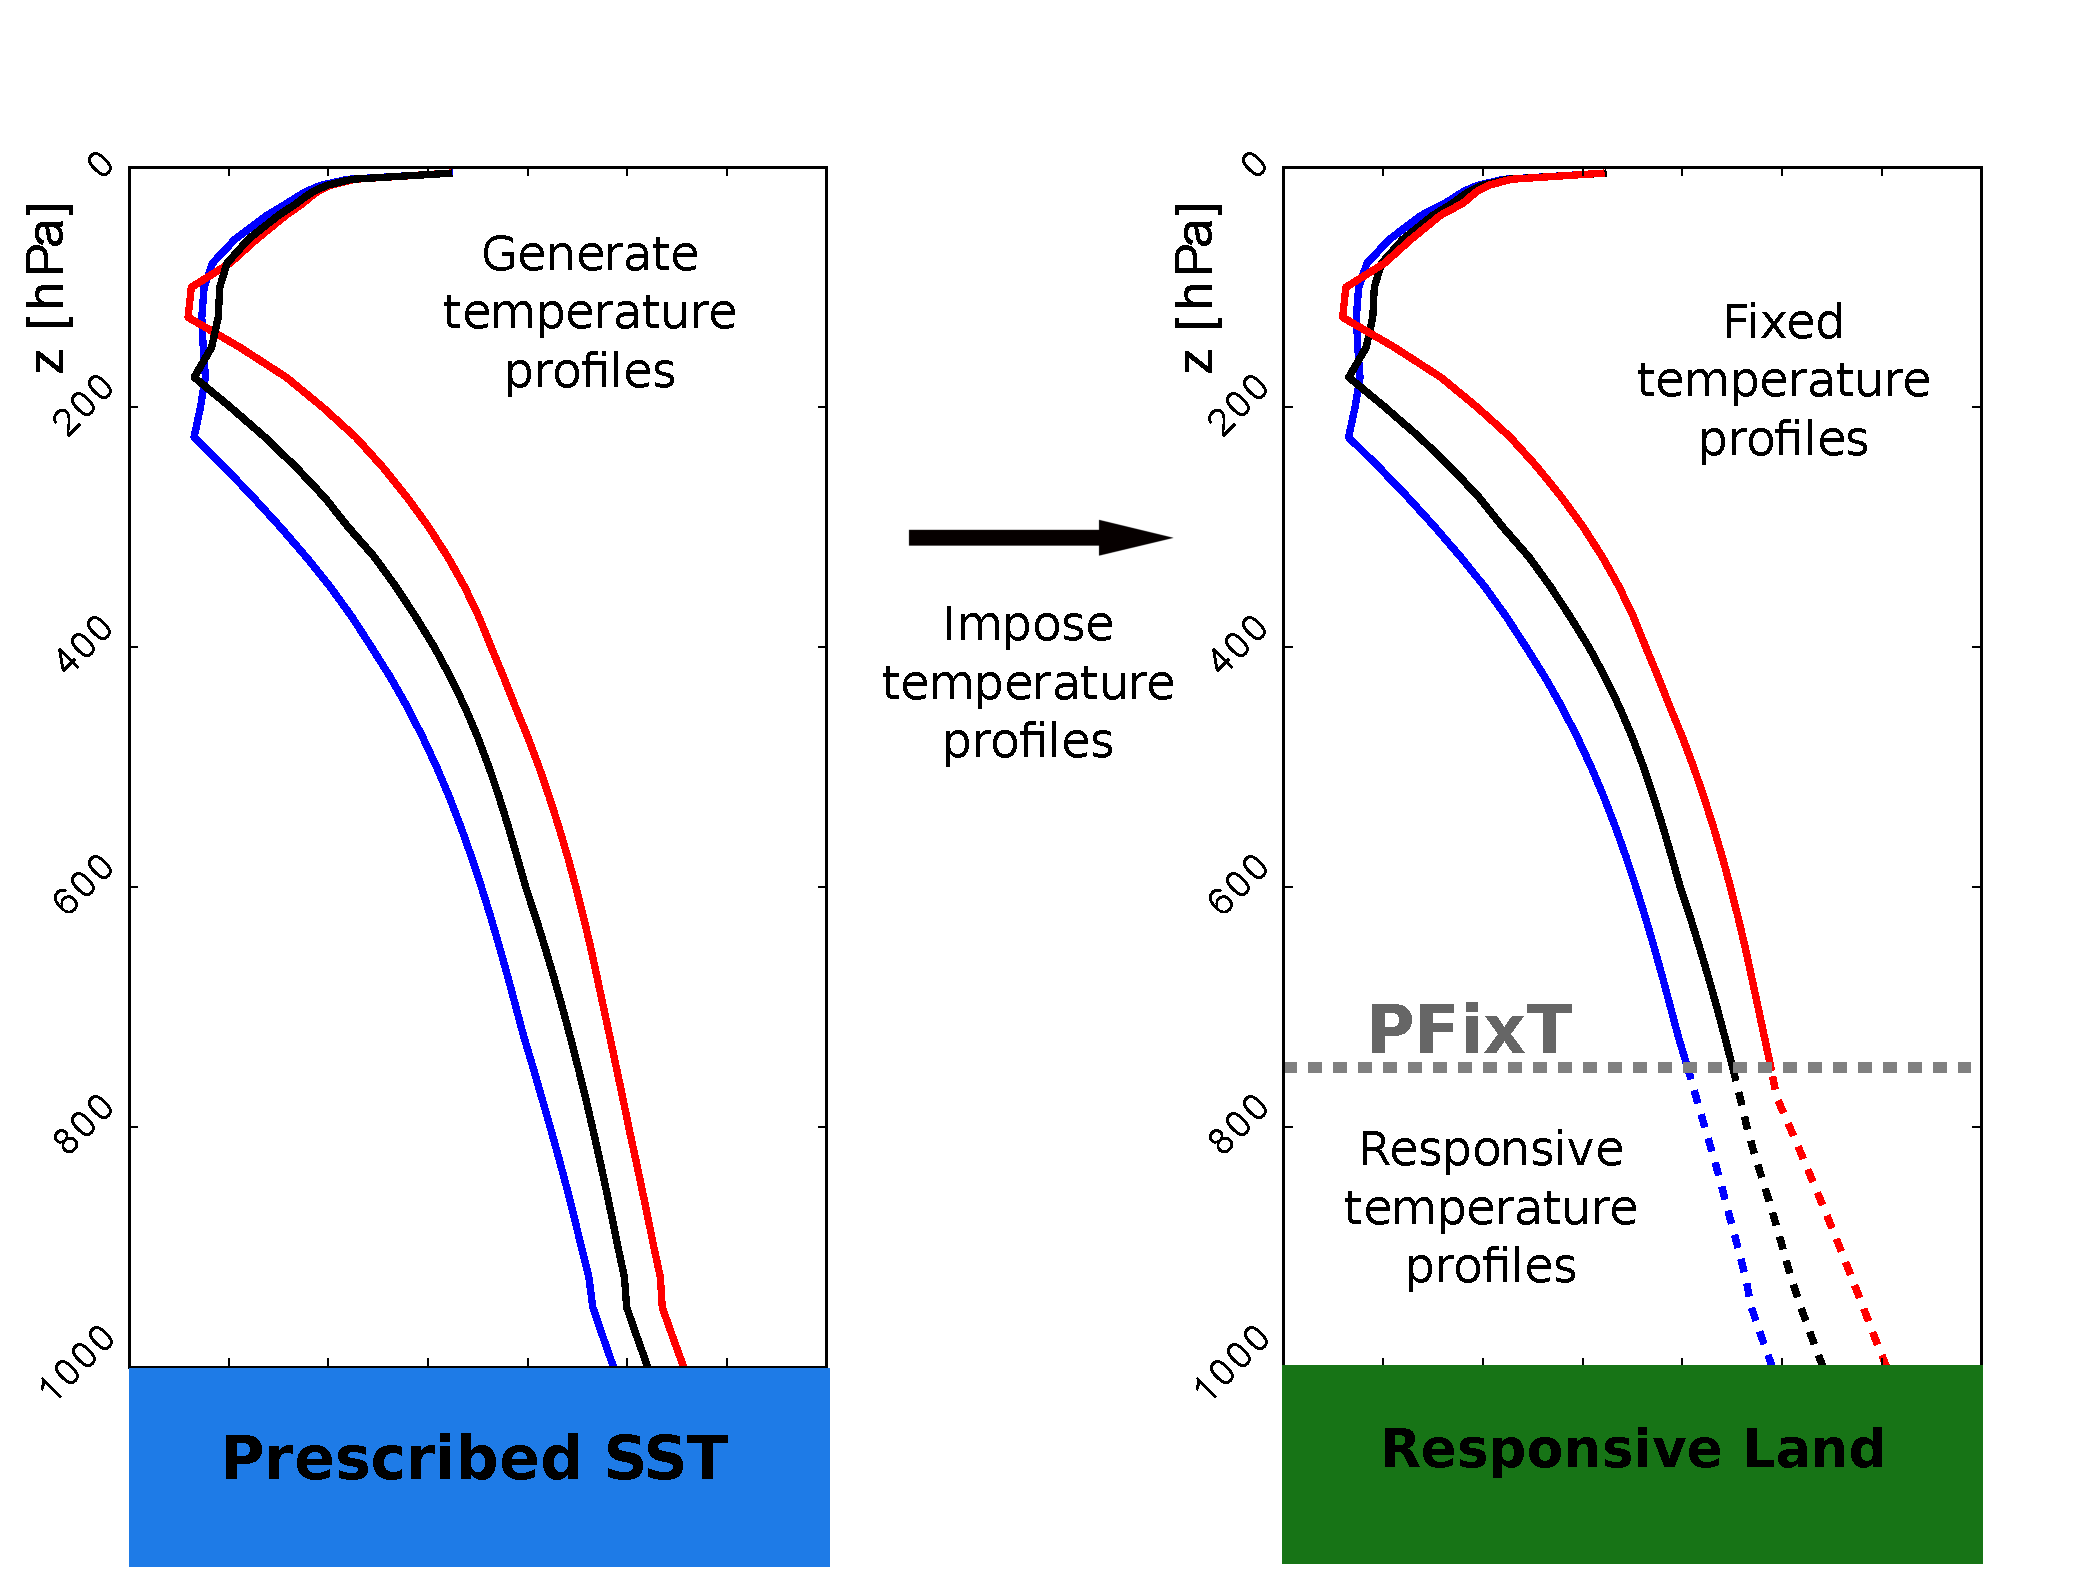
\includegraphics[width=0.9\textwidth,trim={0cm 0cm 0cm 
0cm},clip=true]{scm_wtg_schem.eps}
\caption{Schematic of the Single Column Model Weak Temperature Gradient mode 
experimental setup, showing how the generated temperature profiles are imposed 
above the height PFixT, and the lower atmosphere and surface respond.}
\label{fig:scmschem}
\end{figure}

As we will see this model setup offers some useful insights into the problem, 
but the idealized nature of the model does lead to a number of problems.  From a 
more theoretical viewpoint, RCE models have not been studied extensively over 
land surfaces. Although not in the scope of this study, further work on the 
validity of RCE over a surface with restricted water would be of interest. For 
this study many of the experiments involved small changes in temperatures, to 
simulate those seen in interannual variability.  The model often responded with 
large variability, bringing in to question the stability of the model. It will 
be shown that timeseries of the surface temperatures exhibit chaotic bevavhiour, 
arising from the interaction of the convection and radiation schemes. It remains 
unclear how realistic some of this behaviour is, and leads to inconclusive 
results.

\subsection{Tropospheric response to imposed SSTs in a single column}
\label{trop_response_ocean}

Before we begin our land surface response experiments we must generate the 
tropospheric temperature profiles above an ocean surface. By looking at 
temperature profiles as we vary the SST about an average tropical value we can 
test the model response against the expected theoretical response. We chose an 
SST value of \SI{26}{\degreeCelsius} as the average profile, which is 
appropriate for the tropics. For this section we look at both small and large 
anomalies from a chosen mean value; large anomalies test the robustness of the 
model and small anomalies are more appropriate for modelling interannual 
variability.

In Figure \ref{fig:scmsstprof_large} (a) we see the temperature profile for a 
wide range of SST values. For each profile the model has been run to 
equilibrium, and an average of the last 100 days is taken. The difference 
between the profiles with increasing and decreasing SST values is more clearly 
shown in Figure \ref{fig:scmsstprof_large} (b). For this plot the mean profile 
was calculated using all values from \SIrange{19}{33}{\degreeCelsius}, and then 
the mean profile was subtracted from each individual profile to give the change 
relative to the mean. This shows the amplification of the anomaly with height.  
For example, with the run forced with \SI{33}{\degreeCelsius}, at the surface 
the temperature is \SI{7}{\kelvin} warmer than the mean, and at 
\SI{200}{\hecto\pascal} the profile is approximately \SI{14}{\kelvin} warmer.  
This amplification of surface anomalies with height is the consequence of the 
profile being close to moist adiabatic, as expected in convecting regions of the 
tropics. The amplification above the ocean surface is also important in the 
communication of SST anomalies from oceans to land. 

\begin{figure}[ht]
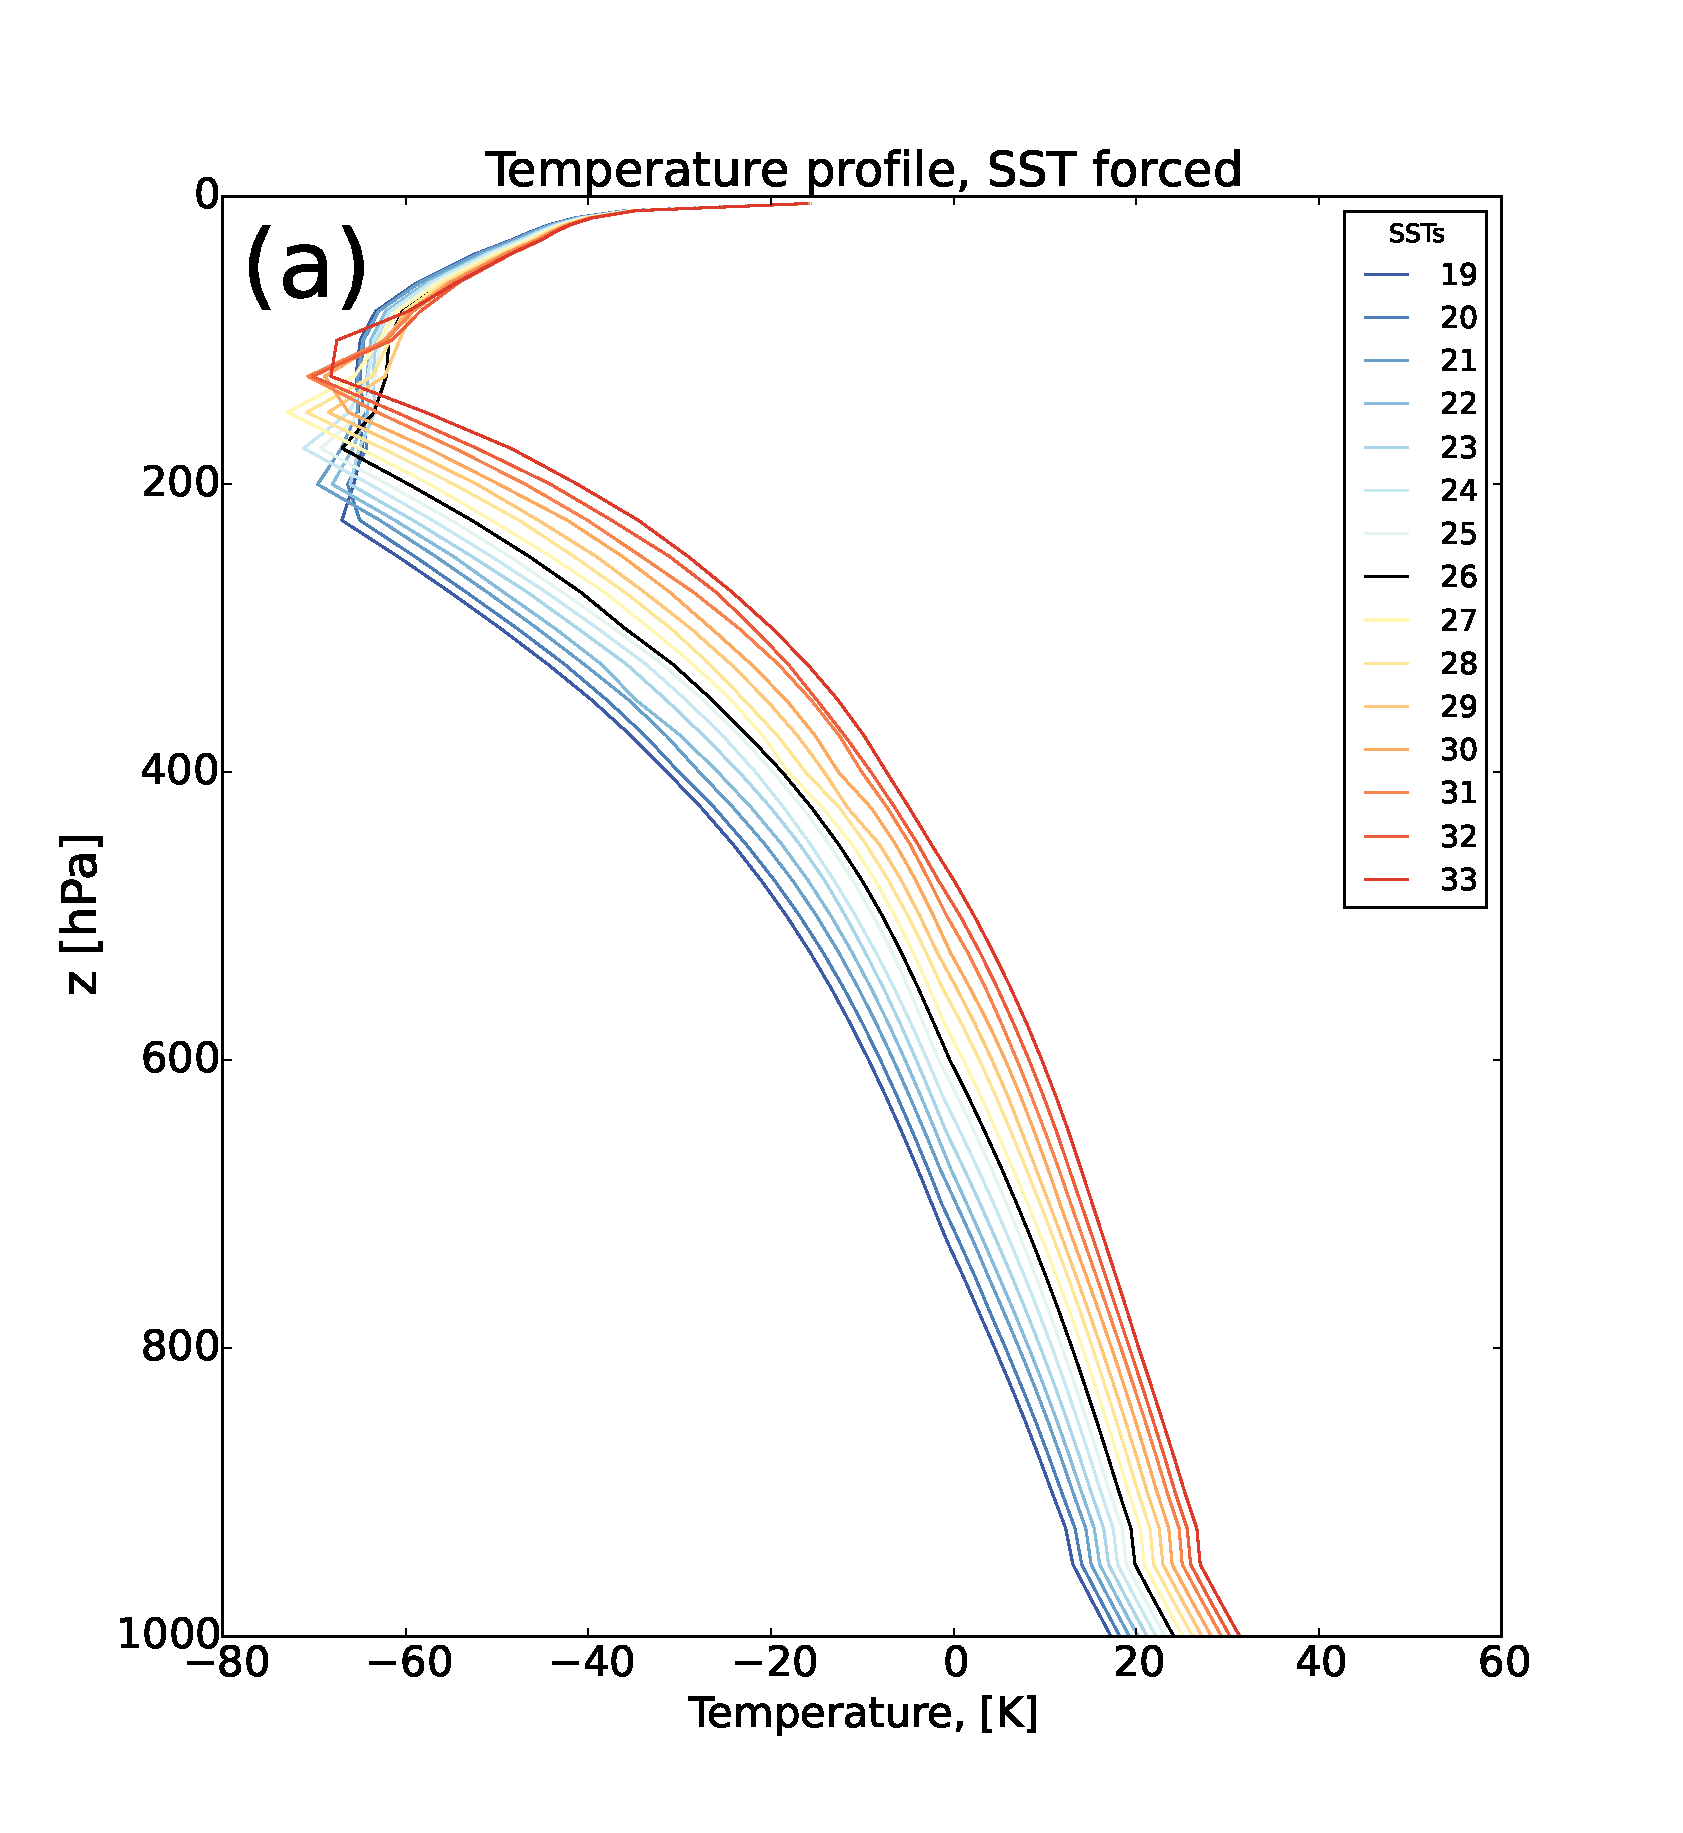
\includegraphics[width=0.5\textwidth]{enso_tempprof_abs.eps}
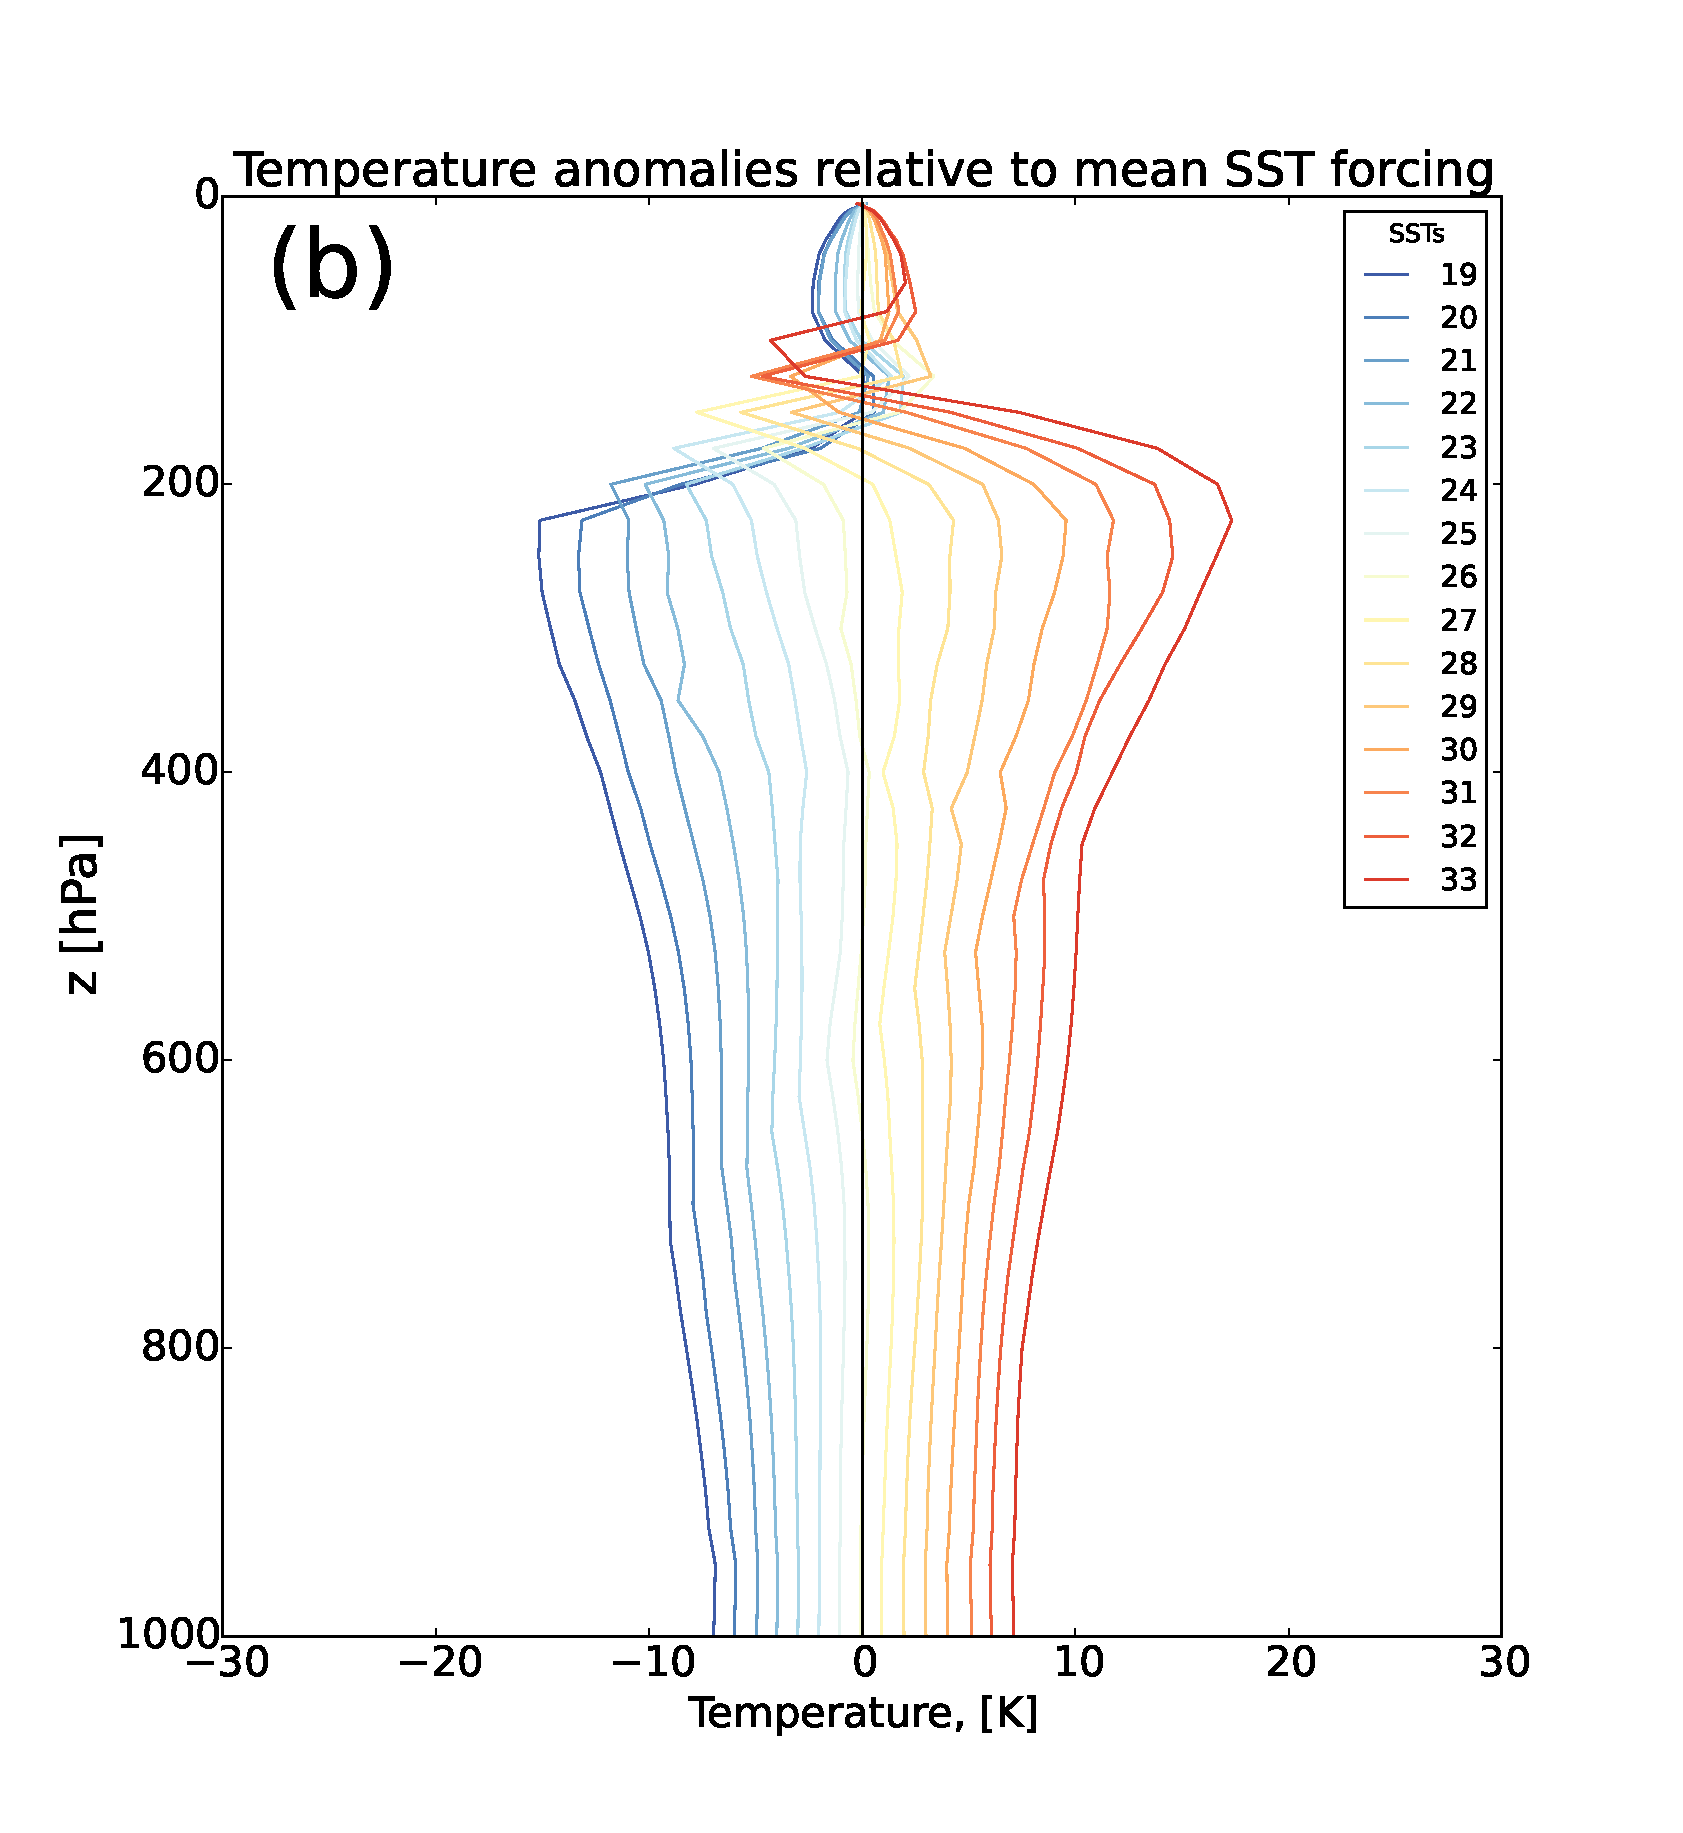
\includegraphics[width=0.5\textwidth]{enso_prof_temp_anom.eps}
\caption{(a) Temperature profiles in the single column model above an ocean 
	surface, for SSTs from \SI{19}{\degreeCelsius} to \SI{34}{\degreeCelsius}, 
(b) Temperature anomalies relative to the mean profile.}
\label{fig:scmsstprof_large}
\end{figure}

From Figure \ref{fig:scmsstprof_large} (b) it appears the temperature profiles 
are largely moist adiabatic, but we can confirm that by plotting the moist 
adiabats, see Figure \ref{fig:scmsstprof_ma}. The moist adiabat is calculated 
for each SST, then as with the model response the anomalies are taken relative 
to the mean of the moist adiabats for all SSTs. We see that that model follows 
the moist adiabat closely from \SIrange{1000}{600}{\hecto\pascal}, after which 
they diverge slightly with the model showing less amplification. From this we 
can conclude that for a wide range of SST values, and for large differences in 
SST of up to \SI{8}{\kelvin}, the troposphere in the ocean forced column is 
largely moist adiabatic.  We can now compare this to the smaller SST variations 
used to model interannual variability.

\begin{figure}[ht]
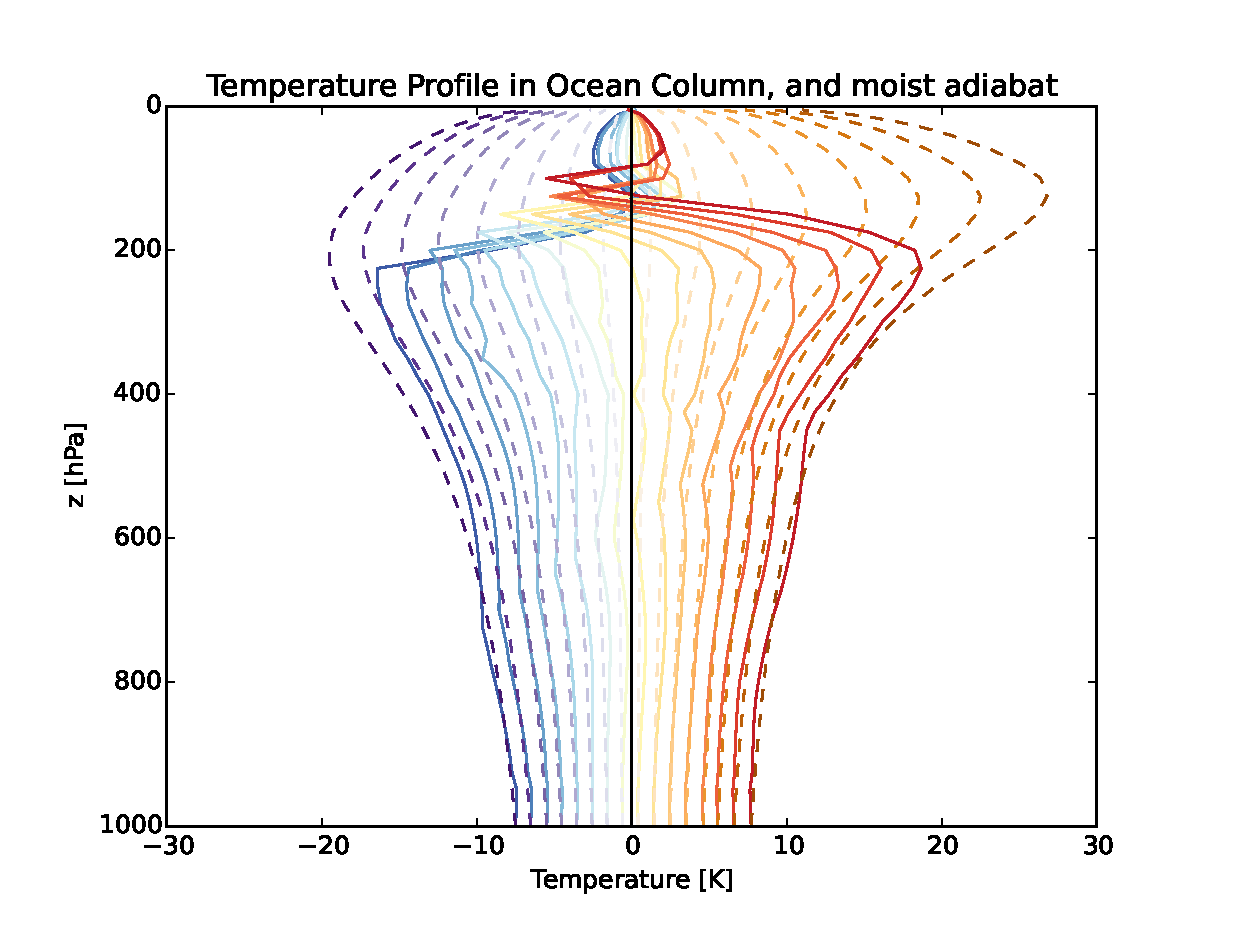
\includegraphics[width=0.5\textwidth]{enso_prof_temp_anom_ma.eps}
\caption{Solid lines; Temperature anomalies relative to mean profile for SSTs 
from \SI{19}{\degreeCelsius} to \SI{34}{\degreeCelsius}. Dashed lines; moist 
adiabat anomalies, the adiabats are calculated for each surface temperature 
(from \SI{19}{\degreeCelsius} to \SI{34}{\degreeCelsius}) and anomalies 
calculated relative to all SSTs.}
\label{fig:scmsstprof_ma}
\end{figure}

The temperature profiles in Figure \ref{fig:scmsstinc_prof} showing small 
changes in SST values don't reveal anything unexpected, as any differences are 
too small to discern at this scale. The profiles are similar to 
\ref{fig:scmsstprof_large}a) with the exception that there is little change in 
the height of the tropopause for small SSt changes. As with Figure 
\ref{fig:scmsstprof_large} b) the anomalous profiles were calculated using the 
mean of all SSTs, the result is Figure \ref{fig:scmsstinc_prof} b). For 
reference the moist adiabat for the warmest and coldest SST anomalies are 
included as dashed lines. The plot shows that relative amplification in the 
upper troposphere still occurs but with greatly increased variance relative to 
the mean. The plotted moist adiabats show that the profiles are still largely 
moist adiabatic, although for individual runs they can be up to 
\SI{0.5}{\kelvin} warmer or cooler than the moist adiabat. The increased 
variance also mostly occurs above \SI{600}{\hecto\pascal}. The variability in 
the temperature profiles may have consequences for the modelled interannual 
value of the land/ocean contrast. The control of tropospheric temperatures by 
the ocean surface is necessary for temperature anomalies to be communicated to 
land surfaces, and demonstrates that variations in SST may not directly 
correspond to tropospheric anomalies.\\
We can look closer at the tropospheric amplification to determine the 
significance of the variations in the temperature profiles for small and large 
anomalies.


\begin{figure}[ht]
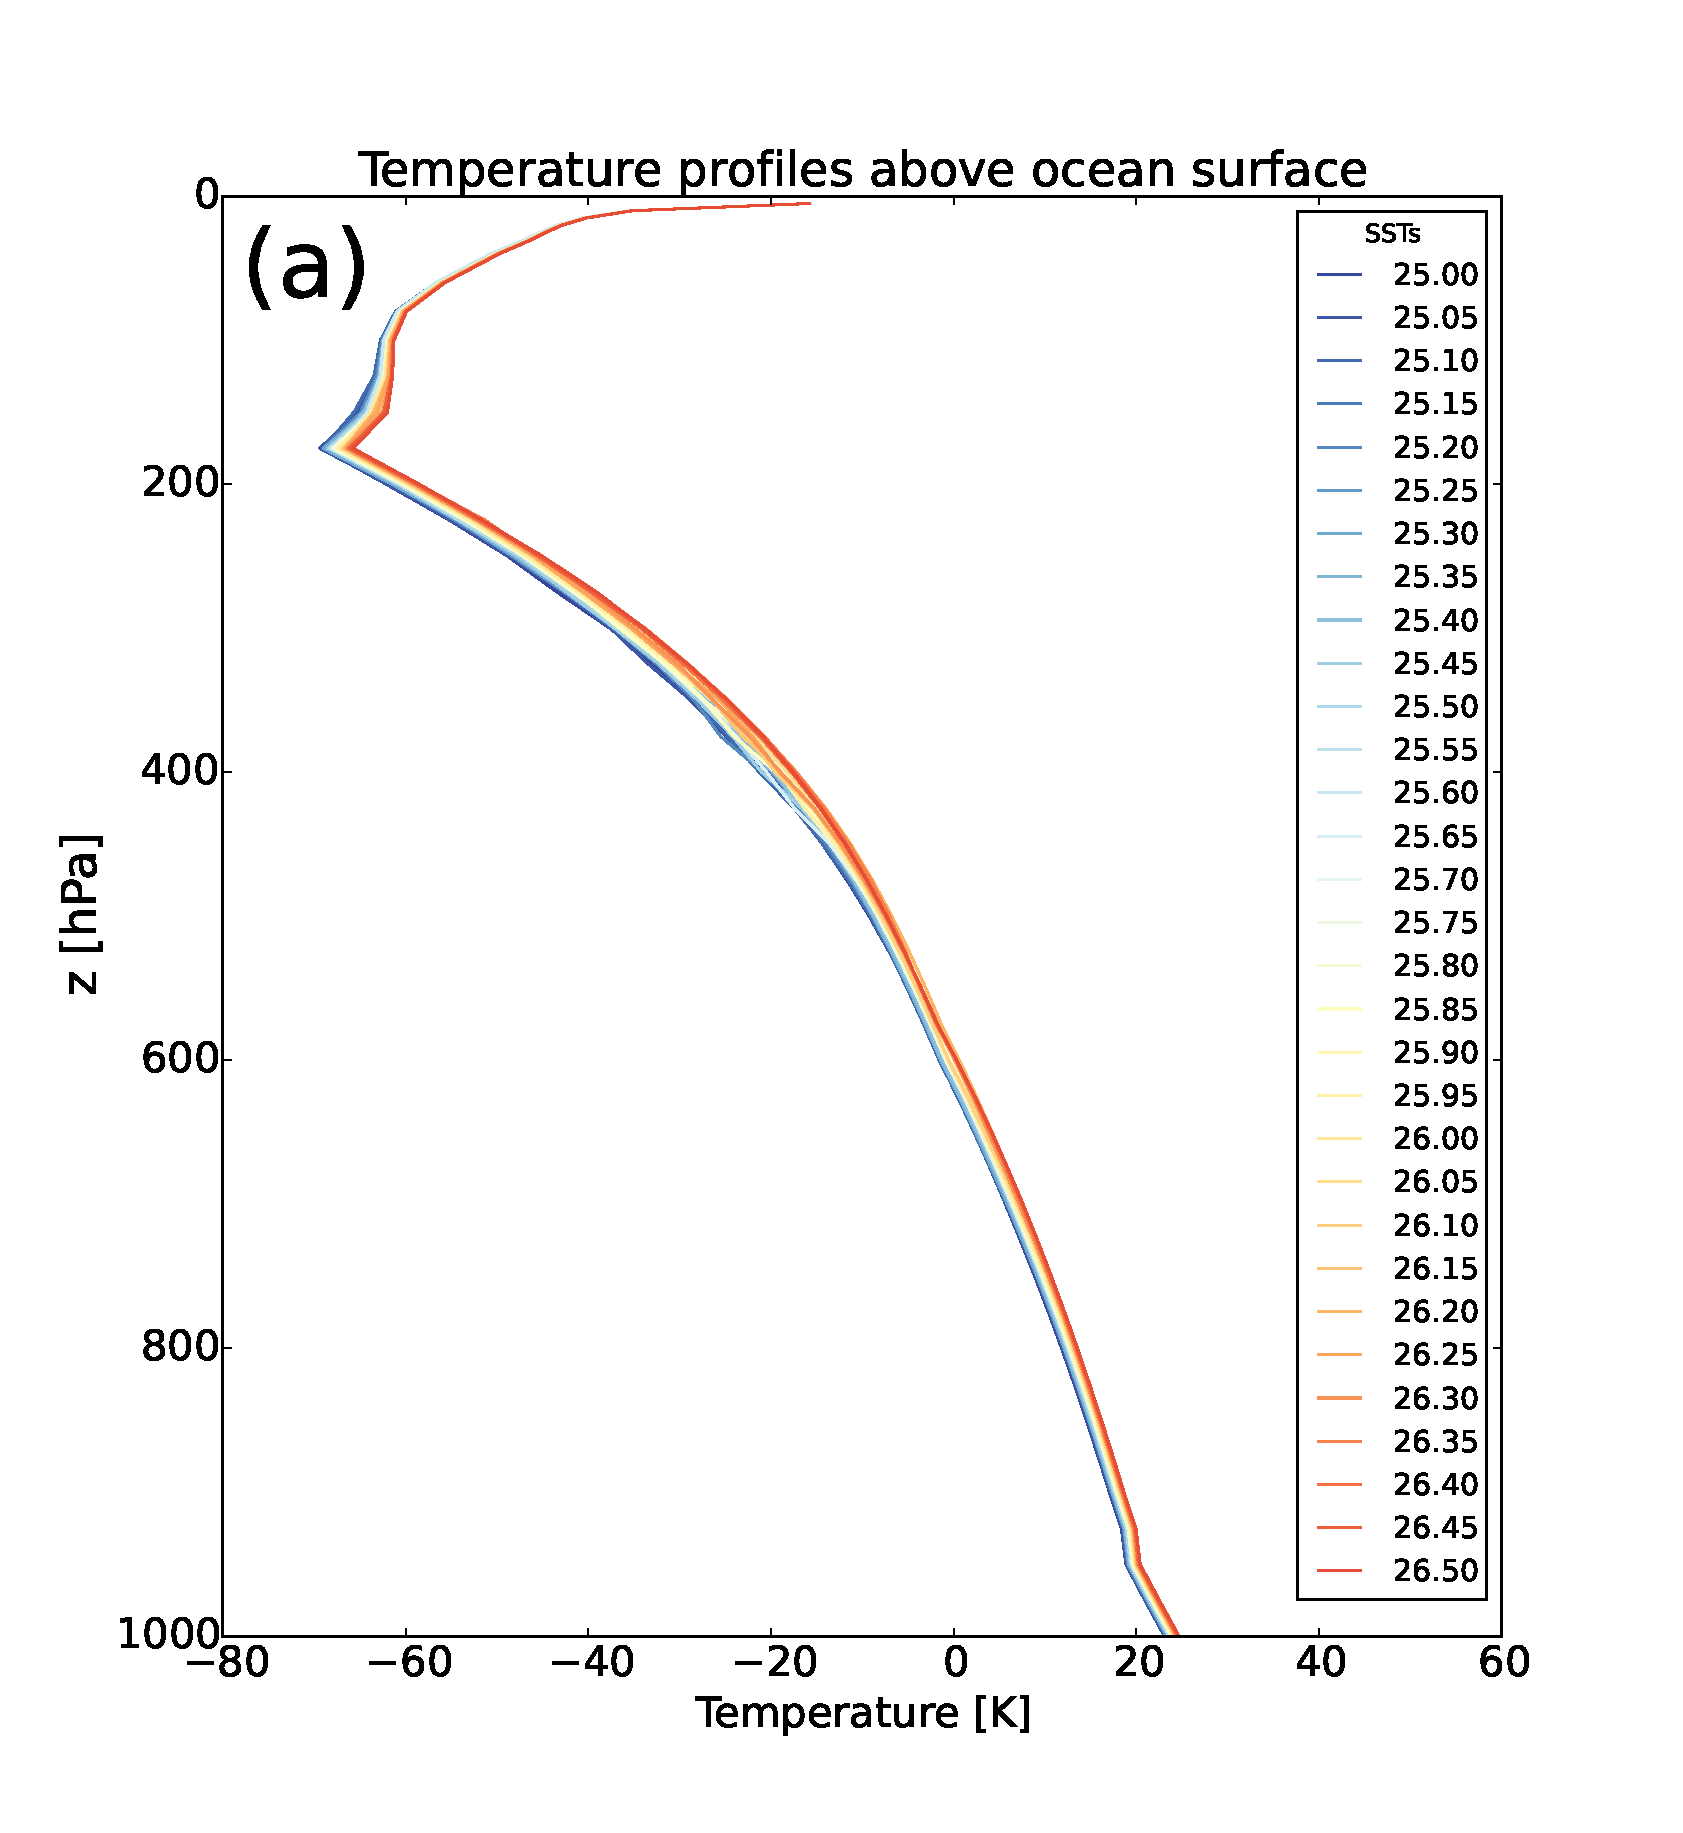
\includegraphics[width=0.5\textwidth]{sstinc_prof_temp_abs.eps}
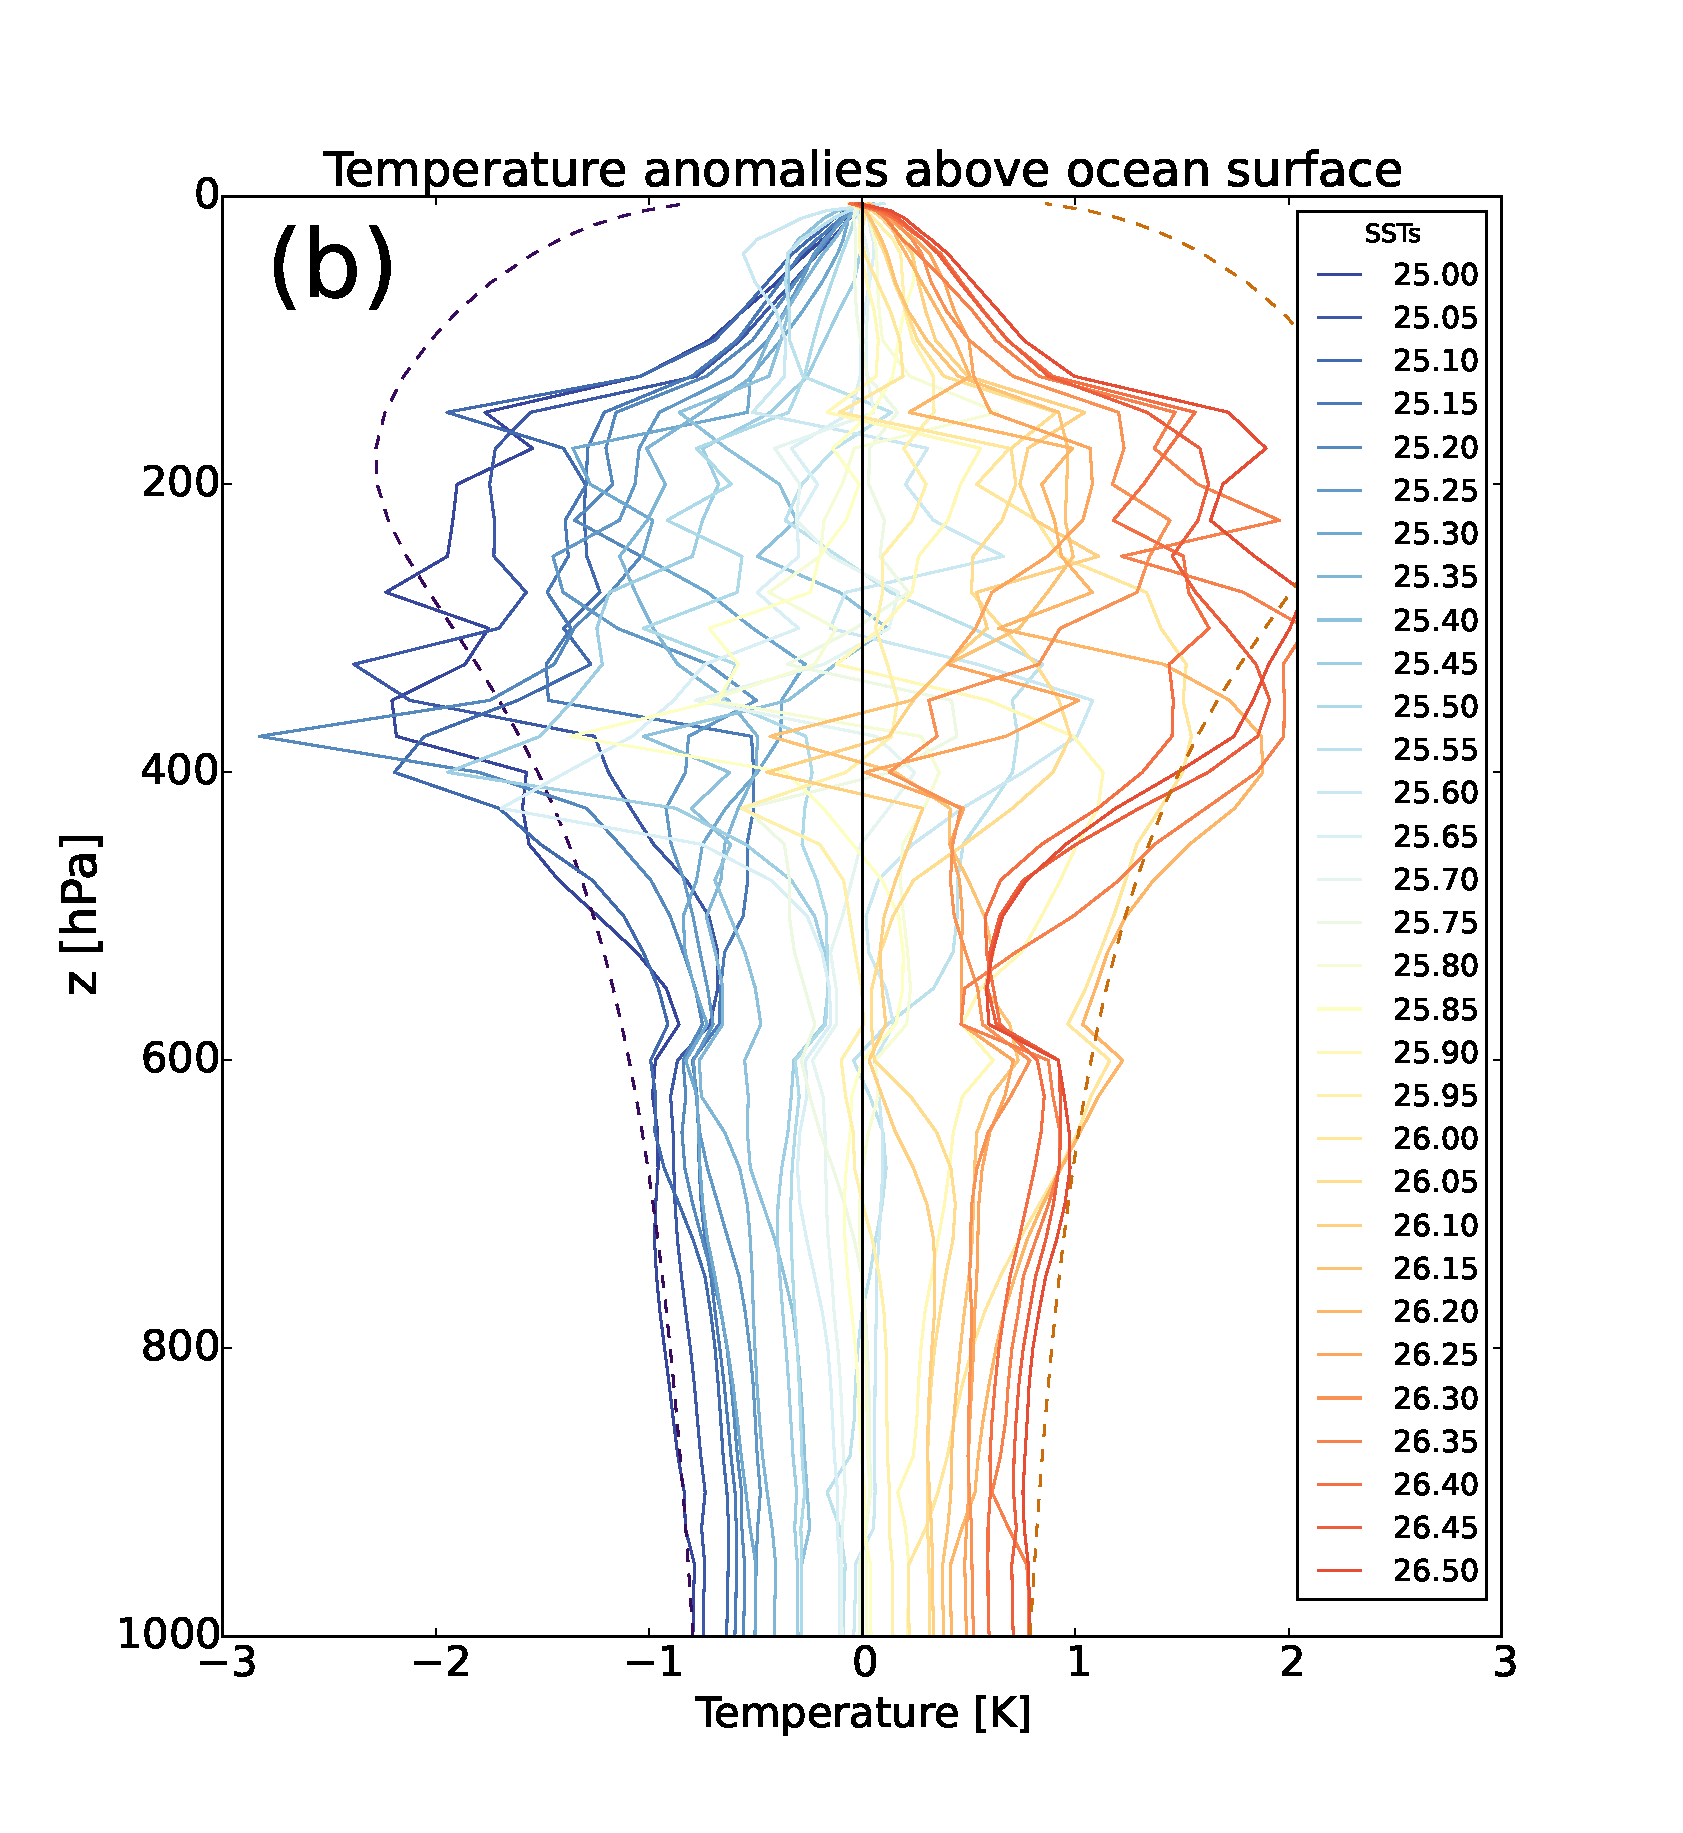
\includegraphics[width=0.5\textwidth]{sstinc_prof_temp_mean_ma.eps}
\caption{(a) Temperature profiles in the single column model above an ocean 
surface, for SSTs from \SI{25.00}{\degreeCelsius} to \SI{26.50}{\degreeCelsius}, 
(b) Temperature anomalies relative to the mean profile. As with Figure 
\ref{fig:scmsstprof_large} the moist adiabat anomalies were calculated for each 
SST, the dashed lines in (b) show the moist adiabat anomalies for the highest 
and lowest SST.}
\label{fig:scmsstinc_prof}
\end{figure}

The magnitude of the tropospheric amplification is more clearly shown in Figure 
\ref{fig:scmsstamp}. For this plot each anomalous temperature profile was 
divided by the SST anomaly used to create it. For example; taking the 
temperature profile created with an SST of \SI{30}{\degreeCelsius}, first the 
anomalous profile was created by minusing the median profile 
(\SI{26}{\degreeCelsius} profile), then the anomalous profile was divided by the 
anomalous SST, in this case the mean SST is \SI{26}{\celsius} so the anomalous 
SST value is \SI{4}{\celsius}.  This gives a ratio of amplification at each 
level, starting at unity at the surface and increasing to above 2 at 
\SI{300}{\hecto\pascal}, as shown in Figure \ref{fig:scmsstamp}.  In this way we 
get a measure of the amplification of the SST anomaly with height relative to 
the mean value.  A value of 2 at \SI{300}{\hecto\pascal} would indicates that a 
surface anomaly of \SI{1.5}{\kelvin} would lead to a \SI{3}{\kelvin} anomaly at 
that height.  

From Figure \ref{fig:scmsstamp} (a) we see that for large SST changes the 
positive anomalies (reds) show a larger amplification than the negative 
anomalies (blues), in addition the tropopause is higher for the positive 
anomalies leading to a difference at \SI{200}{\hecto\pascal}. The picture is 
much less clear in \ref{fig:scmsstamp} (b). There doesn't appear to be a 
significant difference between the positive and negative anomalies, however the 
overall values do seem to be similar at around 2-3. From these plots we can 
conclude that the amplification of surface temperature is fairly robust for a 
range of scenarios, for large SST anomalies there is greater amplification for 
warm anomalies, and there's a high level of variability for small SST anomalies.

\begin{figure}[ht]
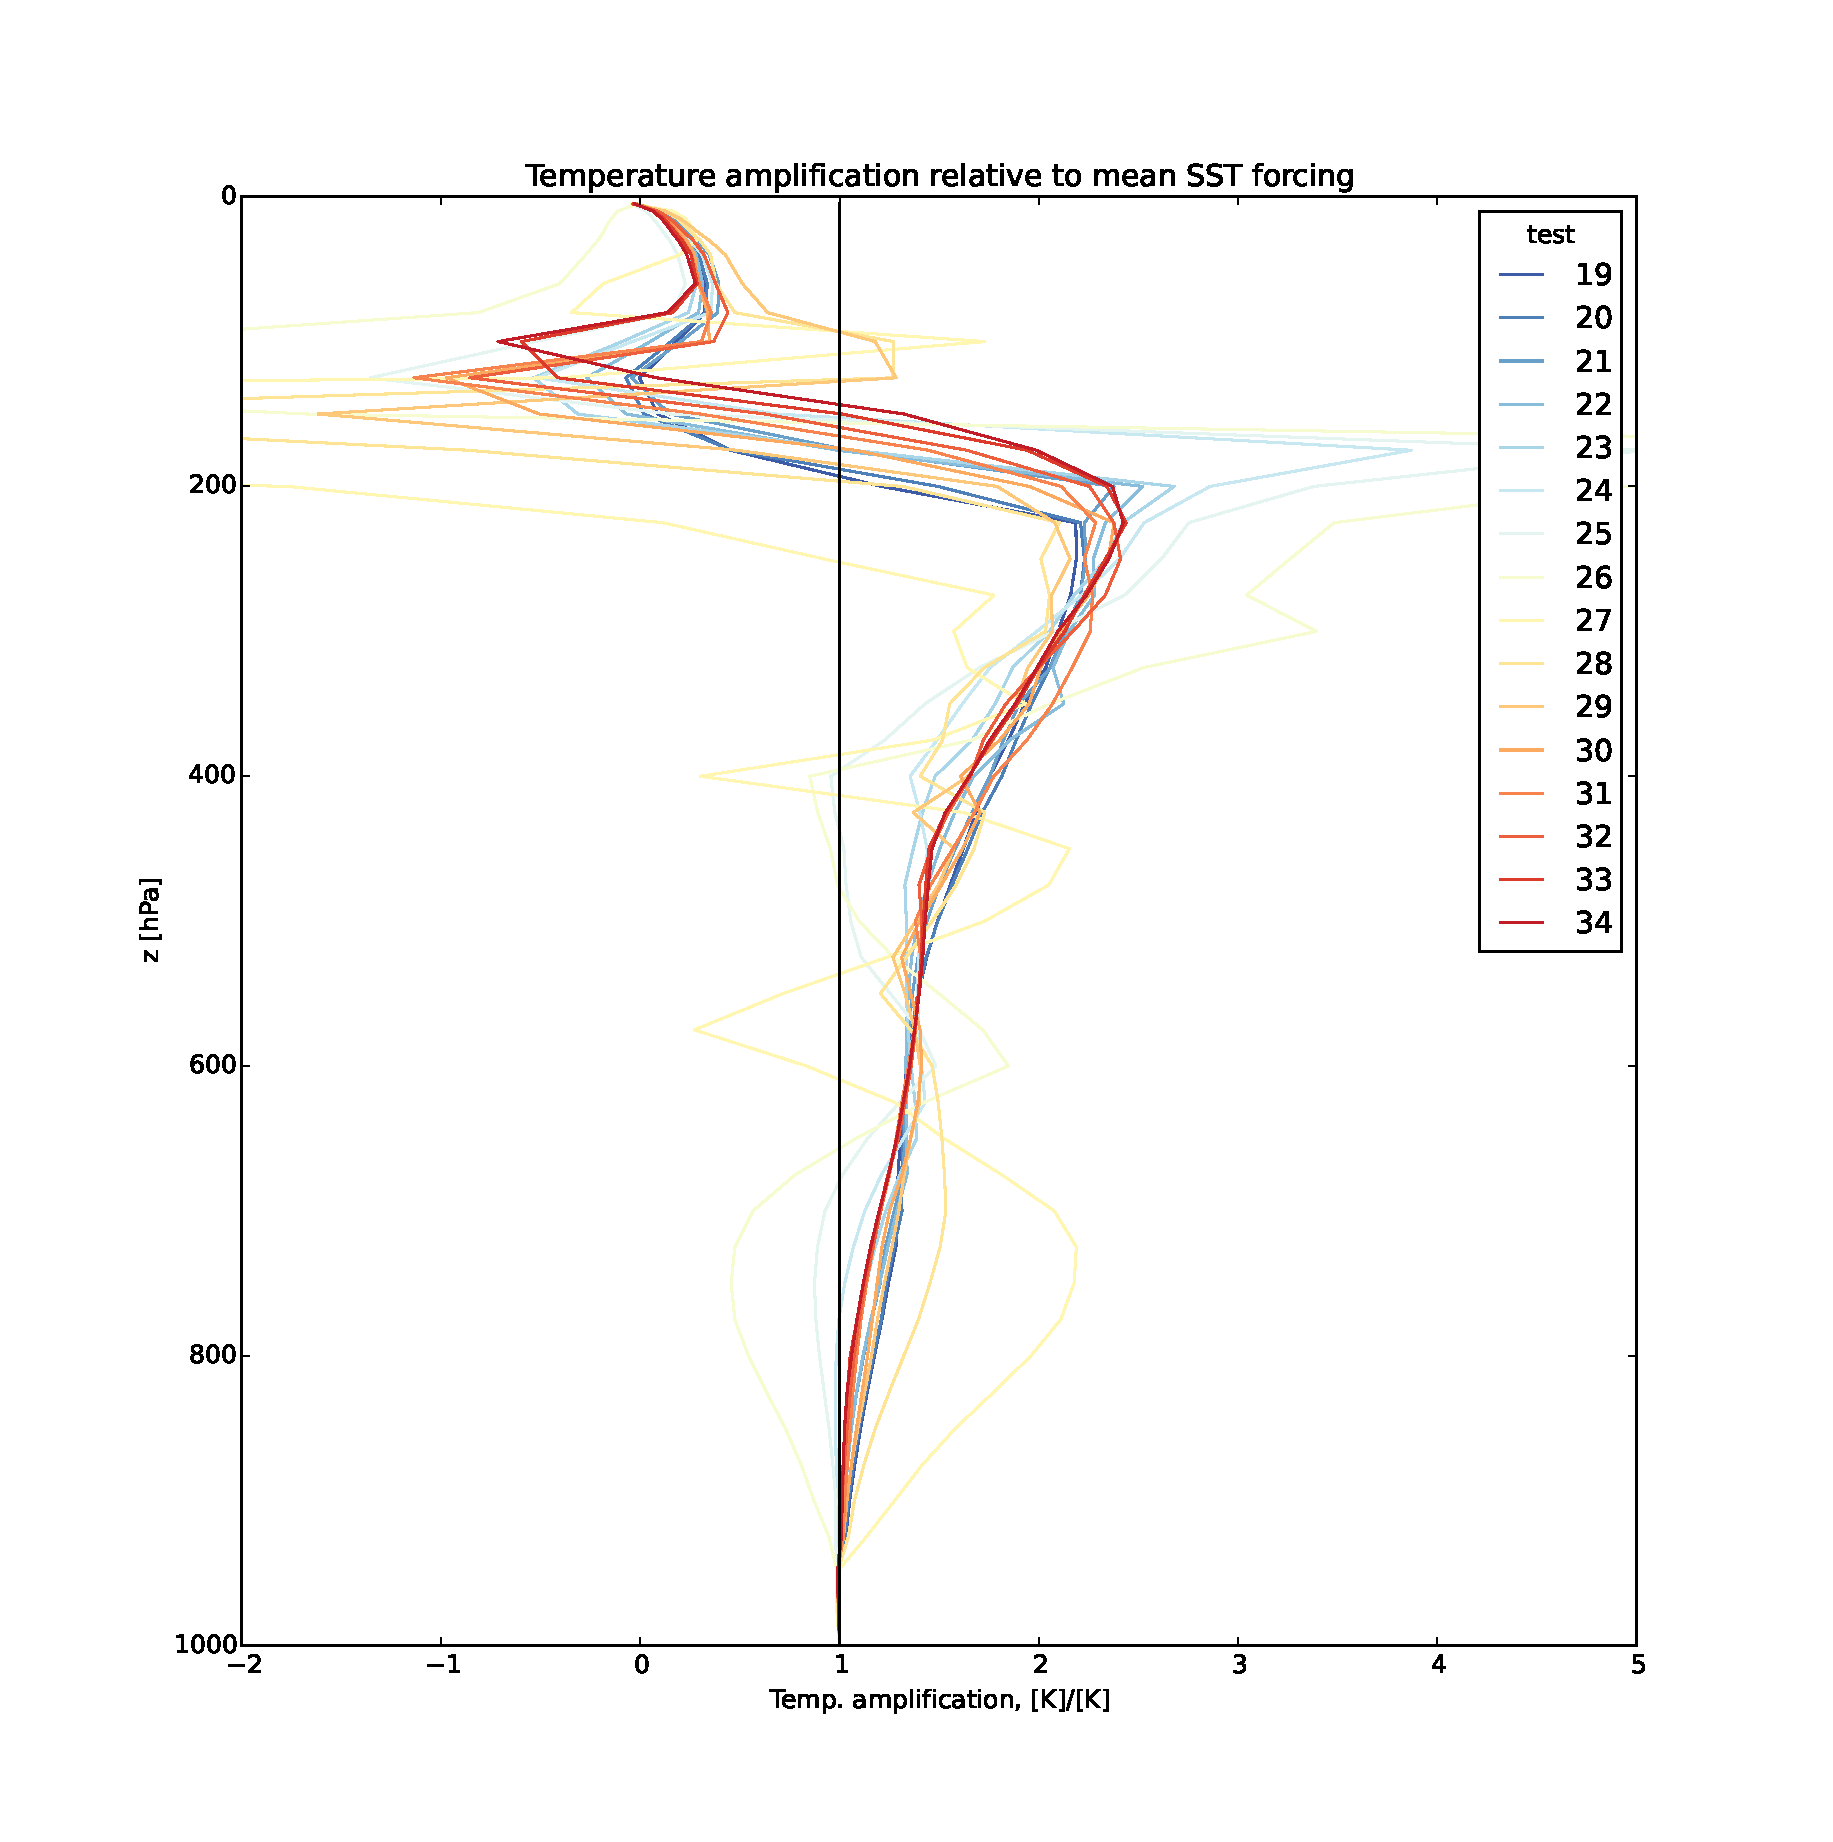
\includegraphics[width=0.5\textwidth]{enso_prof_ampratio_mean.eps}
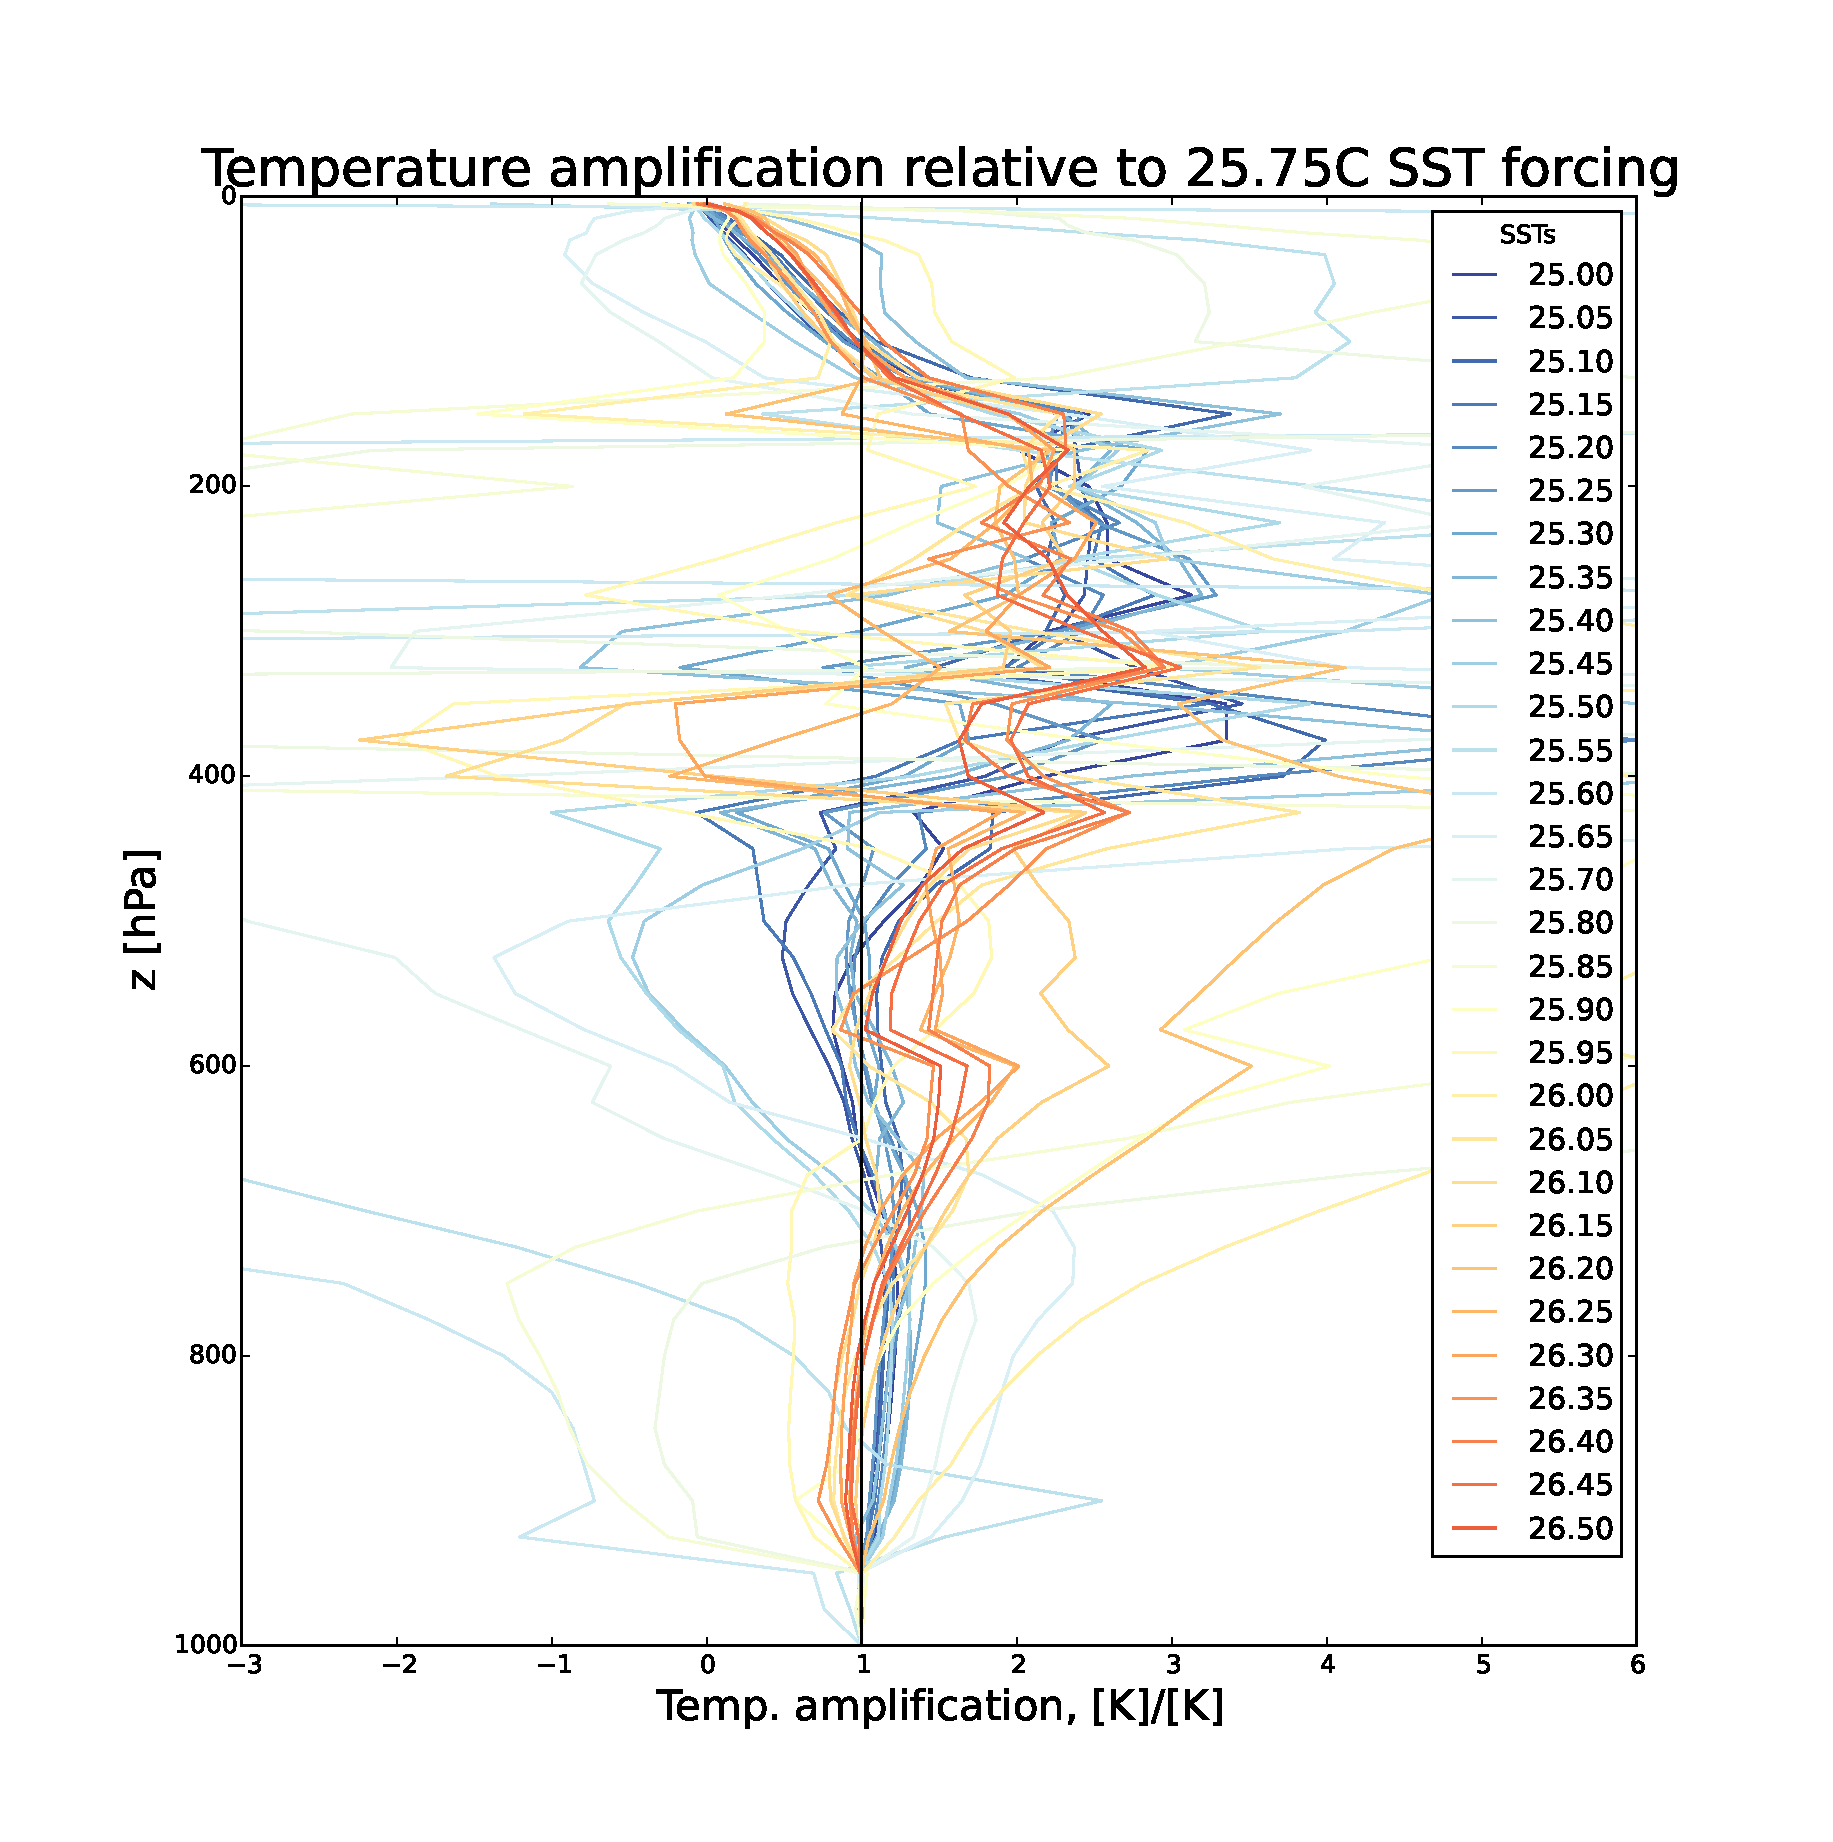
\includegraphics[width=0.5\textwidth]{sstinc_prof_ampratio_mean.eps}\\
\caption{Amplification of the temperature profile relative to the mean profile 
	for SSTs from (a) \SI{19.00}{\degreeCelsius} to \SI{34.00}{\degreeCelsius} 
and (b) \SI{25.00}{\degreeCelsius} to \SI{26.50}{\degreeCelsius}. To calculate 
the amplification each anomalous profile was divided by the SST anomaly used to 
generate that profile.}
\label{fig:scmsstamp}
\end{figure}

In order to study the land surface temperature response to a tropospheric 
forcing a single column model allows us to vary parameters of the land surface 
properties while controlling the tropospheric forcing.  We begin by generating 
the temperature profiles above an ocean forced column by prescribing a range of SSTs 
and running the model to equilibrium.  The focus of our study is interannual 
variability, so we chose an SST value of \SI{26}{\degreeCelsius} as the mean 
profile -- which is appropriate for a tropical profile -- then the SST was 
varied by fractions of a degree above and below the mean value to simulate the 
magnitude of interannual variability. For these experiments we're not concerned 
with the rate of the land or ocean response so at each value the model was run 
to equilibrium, with the equilibrium value comparative to an annually averaged 
value from observations or a GCM.  In addition to these small SST changes the 
model was run with \SI{1}{\degreeCelsius} increments from 
\SI{19}{\degreeCelsius} to \SI{34}{\degreeCelsius}, to test the response of the 
model over a wide range of SSTs.

We have looked at the tropospheric temperature response to imposed SSTs in the 
single-column model. The model largely follows changes in the moist adiabat for 
relatively large SST changes, and for small difference that are comparable to 
interannual variability we see a large amount of variance but a similar 
tendency. The next step is to use these profiles above a land surface, and to do 
that we are going to utilise the Weak Temperature Gradient approximation.

\subsection{The Weak Temperature Gradient Approximation}
The Weak Temperature Gradient (WTG) approximation is used to parameterize the 
large scale tropical circulation. Due the small Coriolis force near the equator 
the tropical troposphere is unable to maintain strong temperature gradients, 
allowing areas of strong convection to control the tropical tropospheric 
temperatures.  The assumption we use is that the uniformity of tropospheric 
temperatures in the tropical band means that temperature profiles above land and 
ocean are controlled by convecting regions of the ocean. This allows us to use 
the profiles from an ocean forced column above land.

The single-column model can be run in WTG mode. In this mode a temperature 
profile is imposed in the free troposphere above a specified height, and the 
temperature below is able to adjust. Similar model setups have been used in a 
number of previous studies (e.g. \citealt{Sobel2000}, \citealt{Lintner2005}, 
\citealt{Ramsay2011}), although none have specifically looked at the land/ocean 
contrast.

\subsection{Values of land ocean contrast modelled with a single column model}
\label{sec:scmrlo}

We have discussed the temperature profiles above an ocean surface and introduced 
the WTG approximation which allows us to use upper level profiles as boundary 
conditions above a land surface.  We can now look at the response of a land 
surface to the imposed upper level temperature profiles, and subsequently 
calculate the modelled land/ocean contrast.  For the tropospheric forcing we 
will be using the temperature profiles created with SSTs that were centred on 
\SI{25.75}{\celsius} and varied in \SI{0.05}{\celsius} increments from 
\SIrange{25.00}{26.50}{\celsius}. These values were used to represent 
interannual variability. As mentioned, the height above which the temperature 
profile is fixed can be assigned, and is designated as PFixT (Pressure above 
which to Fix the Temperature profile). Surface soil moisture is a boundary 
condition, with the land surface is represented simply by changing the 
evaporative fraction and using a small mixed layer depth.

Figure \ref{fig:scm_tlandsst} shows the SST anomalies (from the mean value of 
\SI{25.75}{\celsius}) plotted against the resulting $T_{land}$ anomalies 
(calculated from the mean value of $T_{land}$ for all SSTs) for three 
evaporative fractions and a PFitxT value of \SI{600}{\hecto\pascal}. The lines 
are the linear regressions between the SST and $T_{land}$. The regression lines 
are a useful visual representation of the regression coefficient, $R_{l/o}$, 
used to measure the interannual land/ocean contrast. The black dotted line is 
the one-to-one line; any regression line that is steeper implies an $R_{l/o}>1$.  
What we see are $R_{l/o}$ values greater than one, i.e. the land ocean contrast 
exists, and the steepness increases with decreasing evaporative fraction (drier 
surface). It should be noted for absolute temperatures we would also see the 
$T_{land}$ values increasing for drier surfaces, but we are concerned here with 
deviations around the mean. 

\begin{figure}[ht]
\includegraphics[width=0.6\textwidth]{{land_anom_intvar_tsurf_p600}.eps}
\caption{The relationship between $T_{land}$ and SSTs, using anomalies, for 
three evaporative fractions of 0.3, 0.5, and 0.7.}
\label{fig:scm_tlandsst}
\end{figure}


We now have a measure of the land/ocean contrast in the single column model, 
$R_{l/o}$, that we can compare with observations and GCM results, and we can use 
the simplified model to see what factors are controlling $R_{l/o}$. In Table 
\ref{tab:scmrlo} are values of $R_{l/o}$ for different evaporative fractions and 
PFixT values. Firstly, we note that the magnitudes of $R_{l/o}$ are comparable 
to the observational and GCM values seen in Table \ref{tab:allstats}. The 
single-column model's values range from 1.11 to 1.63, compared to observation 
and GCM tropical values of 1.19 to 1.35, or global values of 1.26 to 1.50.  
Deconstructing the value of $R_{l/o}$ somewhat, we can look at the values of the 
correlation of land/ocean temperatures and the ratio of standard deviations.  
Some of the single-column model results compare well to the observations and GCM 
tropical values, such as for an evaporative fractions of 0.5 the correlations 
are 0.77 to 0.79 and ratio standard deviations are 1.58 to 1.84, compare to 
obs/GCM correlations of 0.81 to 0.85 and ratio of standard deviations of 1.37 to 
1.48. This tells us that single-column model exhibits slightly higher difference 
  in the land/ocean variance, but overall the $R_{l/o}$ is a metric that is 
  comparable between the simple models and the observations and GCM results.

\begin{center}
	\begin{table}[ht]
		\caption{Land/Ocean contrast, as measured by $R_{l/o}$, in single column 
		model using the WTG approximation over land surfaces. The correlation 
	and Ratio of standard deviations are calculated with the SSTs used to create 
the forcing temperature profiles, and the resulting land surface temperature  
from that profile}

		\label{tab:scmrlo}
		\scriptsize
	\begin{tabular}{ l  c  c  c }
		\textit{Evap Fraction}		& 0.3   & 0.5  & 0.7 \\ \hline
		\textbf{PFixT 800hPa}\\%\hline
		$R_{l/o}$  							& 1.41  & 1.43 & 1.18\\ %\hline
	Corr.							& 0.57  & 0.78 & 0.64\\ %\hline
	Ratio STD           			& 2.48  & 1.84 & 1.60\\ \hline
		\textbf{PFixT 700hPa}\\%\hline
		$R_{l/o}$  							& 1.39  & 1.30 & 1.15\\ %\hline
	Corr.							& 0.50  & 0.77 & 0.76\\ %\hline
	Ratio STD           			& 2.76  & 1.68 & 1.52\\ \hline
		\textbf{PFixT 600hPa}\\%\hline
		$R_{l/o}$  							& 1.63  & 1.25 & 1.11\\ %\hline
	Corr.							& 0.70  & 0.79 & 0.78\\ %\hline
	Ratio STD           			& 2.35  & 1.58 & 1.42\\ \hline
	\end{tabular}
	\end{table}
\end{center}

Now that we have a metric to compare our simplified model with previous results 
we can begin to investigate the factors controlling the land/ocean contrast. In 
Table \ref{tab:scmrlo} two parameters have been tested; the evaporative fraction 
and PFixT. In contrast the value of PFixT does not show a consistent influence 
on $R_{l/o}$. It is possible that PFixT could influence the value of $R_{l/o}$; 
as the pressure at which the profile remains fixed decreases there is more 
potential for the temperature below this to vary.  That PFixT had no clear 
influence on $R_{l/o}$ implies the variation in temperature below the level of 
the fixed temperature profile is not being significantly impacted by the 
specifics of the model setup.  This is a positive outcome, as a dependence of 
$R_{l/o}$ on PFixT would indicate a dependence on a non-physical model 
parameter. Instead we see that we can simulate control of the tropical 
troposphere by tropical oceans and get robust values of $R_{l/o}$.
The evaporative fraction was found to be the strongest controlling factor of the 
value of $R_{l/o}$, in all scenarios a decrease in evaporative fraction lead to 
an increase in $R_{l/o}$.  


Overall the values of $R_{l/o}$ are within a realistic range, from 1.1 to 1.6.
Even for the very moist surface -- an evaporative fraction on 0.7 -- the values 
are similar the tropical values from observations ($R_{l/o, obs} =1.19$), and 
the ENSO-Slab run ($R_{l/o, enso} =1.17$), while the CMIP5 ($R_{l/o,cmip} 
=1.35$) and the AMIP run ($R_{l/o, amip} =1.26$) tropical values are closer to 
corresponding values for an evaporative fraction of 0.5. Looking at how the 
evaporative fraction is controlling the $R_{l/o}$ values we again deconstruct 
$R_{l/o}$ into correlation and ratio of standard deviation. It is primarily the 
ratio of standard deviation which is causing the increase in $R_{l/o}$ with 
decreasing evaporative fraction, as the correlation between the land and ocean 
columns doesn't change significantly.  Although we can't measure changes in the 
observation and GCM values of the ratio of standard deviation or correlation 
with changing surface moisture, we have seen that the tropical values are 
similar to the single column model, with correlation of around 0.8 and ratio of 
standard deviation of around 1.4.  The consistency of these statistics between 
the single column model and observations and GCMs are at least an indication 
that aspects of the relationship between the land and ocean are well represented 
by the single column model. 

The single column model results indicate a strong dependence of the magnitude of 
$R_{l/o}$ on surface moisture availability, modelled with evaporative fraction.  
This will be further explored by comparing the atmospheric profiles of 
temperature above ocean and land surfaces.


\subsection{Lower atmospheric response to a free tropospheric forcing}

We have seen that by using the WTG mode we can force a single-column model with 
tropospheric temperature profiles and model a land/ocean contrast, and it's 
magnitude is comparable to observations and GCMs and dependent on the dryness of 
the land surface.  We will now look at the atmospheric temperature profiles 
above land and ocean and compare the results to existing theories concerning the 
role of atmospheric lapse rates and the land/ocean contrast. The results below 
use a PFixT of \SI{600}{\hecto\pascal} and an evaporative fraction of 0.3. The 
low evaporative fraction (relative to 
0.5 or 0.7) resulted in larger deviations between the temperature profiles of 
the land and ocean forced columns, allowing for easier comparison. The results from 
other runs with different evaporative fractions and PFixT values were similar 
but of different magnitude.\\

\citet{Byrne2013a} outlined a mechanism for the global warming land/ocean 
contrast based on the height of the lifting condensation level (LCL). A 
schematic of the potential temperature ($\theta$) profile above land and ocean 
is shown in the Figure \ref{fig:bo_fig1}.  It demonstrates that in the free 
troposphere the temperature profiles above land and ocean follow the same moist 
adiabatic profile ($\Gamma_m^*$), and then a difference in LCL heights (i.e. the 
point where the profile flattens) results in a temperature difference between 
land and ocean. The difference is dependent on the saturated moist adiabatic 
lapse rate between the ocean and land LCLs. $\Gamma_m^*$ reduces when warming 
occurs, which \textit{increases} the temperature difference between land and 
ocean and creates a land/ocean contrast that exists in transient and equilibrium 
global warming scenarios. We can test the potential suitability of this theory 
for the warming and cooling of interannual variability by looking at profiles of 
potential temperature in the single column model.

\begin{figure}[ht]
\includegraphics[width=0.5\textwidth]{{byrne_ogorman_fig1}.png}\\
\caption{Figure 1 from \citet{Byrne2013a}. A schematic of the potential 
temperature}
\label{fig:bo_fig1}
\end{figure}

Looking now to the results of the single-column model, profiles of $\theta$ are 
shown in Figure \ref{fig:scmthprof} (a). The dashed lines are the profiles from 
the ocean forced column and the solid lines are the land column, and the colours 
correspond to the SST forcing. In the case of the land column, the colours 
represent which profile was imposed in the free troposphere. There is a fairly 
clear difference in the LCL height (\SI{950}{\hecto\pascal} for ocean, 
\SI{925}{\hecto\pascal} for land) over land and ocean which contributes to the 
absolute temperature difference between land and ocean, although we also see the 
land profiles diverging from the ocean \textit{above} the LCL. However the 
absolute difference in temperature is not what we are interested in, we are 
interested in how the change with warming and cooling is amplified over land.  
The important features are more clearly shown in Figure \ref{fig:scmthprof} (b), 
(c) and (d).

In order to see the change in the profiles, Figure \ref{fig:scmthprof} (b) shows 
the anomalous profiles, with the anomalies calculated relative to the mean of 
either all ocean or land columns. Once again the dashed lines are from the ocean 
column and the solid lines are from the land column. It would be expected that 
for the higher and lower land temperatures the profiles have larger anomalies 
than the ocean (i.e. it's comparable to the ratio of standard deviations seen in 
Table \ref{tab:scmrlo}) and plotting the anomalous profiles in this way allows 
us to see at which level the largest amplification is occurring.  The amount of 
variability between each individual run makes it difficult to see any clear 
tendencies, but there are dark blue (red) land profiles that are clearly more 
negative (positive) than the ocean forced column profiles used to force them. To 
clarify the picture all profiles were grouped in to five bins and the same 
analysis was done, as seen in Figure \ref{fig:scmthprof} (c) and (d). We 
essentially have a large positive/negative anomaly, small positive/negative 
anomaly and no anomaly.  

\begin{figure}[ht]
\includegraphics[width=0.5\textwidth]{{land_thetaprof_e3_p600}.eps}
\includegraphics[width=0.5\textwidth]{{land_deltatheta_e3_p600}.eps}\\
\includegraphics[width=0.5\textwidth]{{land_thetaprof_fifth_e3_p600}.eps}
\includegraphics[width=0.5\textwidth]{{land_deltatheta_fifth_e3_p600}.eps}
\caption{Single column model profiles of theta (a), change in theta from mean 
theta value (b). For c) and d) the profiles have been grouped into five bins.  
The SST values range from \SI{25.00}{\degreeCelsius} to 
\SI{26.50}{\degreeCelsius} and the land has an evaporative fraction of 0.3}
\label{fig:scmthprof}
\end{figure}


According to the Byrne and O'Gorman theory there should be a change in the ocean 
column $\Gamma_m^*$ between the land and ocean LCL levels as the profile warms 
and cools. If this process was driving the change in the single column model the 
dashed ocean profiles in Figure \ref{fig:scmthprof} (d) would slope away from 
the zero point, i.e. the anomalies would increase with height, and the larger 
anomalies would slope more than the smaller anomalies. Importantly this would 
occur in between the land and ocean LCL levels, around \SI{950}{\hecto\pascal} 
to \SI{900}{\hecto\pascal}. The ocean profiles do slope away from zero, but not 
enough to explain the land/ocean contrast. The land (solid) profiles show where 
the amplification is occurring.  The largest change in the warmest and coolest 
profiles is occurring around \SI{950}{\hecto\pascal} to \SI{900}{\hecto\pascal}.  
This is due to an increase (decrease) in the height of the LCL with warming 
(cooling). The contrasting $\Gamma_m^*$ (above the LCL) and dry adiabatic lapse 
rate ($\Gamma_d$) (below the LCL) gradients means that a small change in the LCL 
over land leads to large change in the surface temperature. In addition the 
warmest and coolest land profiles also show a deviation away from the ocean 
column moist adiabat above the LCL, around \SI{900}{\hecto\pascal} to 
\SI{800}{\hecto\pascal}, which further amplifies the warming. Although the Byrne 
and O'Gorman theory of the land/ocean contrast was formulated for a global 
warming scenario, where the magnitude of warming is greater, this doesn't mean
it is not applicable to interannual variability. However we have modelled a 
land/ocean contrast with realistic statistics where it does not apply.
To further investigate the land response we will next look at the relationship 
between a range of variables and the surface temperature.



\subsection{Surface Temperature Relationships}

We have seen that while the atmospheric profile of the single column model shows 
some similarities to the global warming lapse rate theory described by 
\citet{Byrne2013a} but ultimately the mechanism appears to be different.  To 
understand the factors controlling the land surface temperature ($T_{land}$) of 
the single column model we will look at relationships between $T_{land}$ and a 
number of variables. 

In section \ref{sec:scmrlo} and Figure \ref{fig:scm_tlandsst} we saw the 
relationship between $T_{land}$ and the SSTs, where the SSTs were used in an 
ocean forced column to generate temperature profiles and the profiles were imposed in 
the free troposphere of a land column to force the surface temperatures.  The 
regression lines represented $R_{l/o}$ and showed the increase of $R_{l/o}$ with 
decreasing evaporative fraction.  A large amount of variability was evident in 
the response of $T_{land}$ to the imposed temperature profile, this is discussed 
further in section \ref{instability}.  Despite the variability,
when using different values of PFixT, domain size, vertical resolution and other 
parameters the model showed very similar relationships between $T_{land}$, SST 
and evaporative fraction. It is evident then that the SSTs are able to 
consistently influence $T_{land}$.

We will now look at how the SST-generated temperature profiles influence other 
variables in the land column, and how these variables relate to $T_{land}$.  We 
will be using anomalies for all variables and for the purposes of calculating 
the mean each evaporative fraction in the land column was treated as a separate 
run.  The SST is from the ocean forced column, all other variables are from the land 
column, forced with free tropospheric temperature profiles. Figure 
\ref{fig:scm_SSTVar} shows the relative humidity, longwave and shortwave 
radiation and precipitation plotted against the SST and $T_{land}$, with the 
correlation values listed in Table \ref{tab:scm_SSTVar}. A similar picture 
emerges for the four variables; the forcing SSTs have at best a very weak 
relationship with the variables in the land column, but there is a strong 
relationship between the variables and $T_{land}$. For example in Figure 
\ref{fig:scm_SSTVar} (a) we see a very weak relationship between SST and 
relative humidity, with the highest correlation being -0.41, then Figure 
\ref{fig:scm_SSTVar} (b) shows a strong relationship between relative humidity 
and $T_{land}$ with correlations from -0.68 to -0.93. Similar relationships are 
seen for longwave and shortwave radiation, and then precipitation has a weaker 
relationship with the surface temperatures. We are not proposing a causal 
relationship between the surface temperatures and the variables, but looking to 
understand how the imposed temperature profiles are influencing the land column.  
The relationships show that while the imposed profiles have a control on the 
surface temperature, as indicated by the correlations in Table \ref{tab:scmrlo}, 
there is a large amount of independent variability in the land column. The 
source of this variability, and its possible effect on the modelled land/ocean 
contrast will be investigated in the following section.

\begin{figure}[ht]
\includegraphics[width=0.5\textwidth]{{land_anom_intvar_rh_p600}.eps}
\includegraphics[width=0.5\textwidth]{{land_anom_intvar_lw_p600}.eps}
\includegraphics[width=0.5\textwidth]{{land_anom_intvar_sw_p600}.eps}
\includegraphics[width=0.5\textwidth]{{land_anom_intvar_precip_p600}.eps}
\caption{Relationship between; relative humidity (a,b), longwave radiation 
(c,d), shortwave radiation (e,f), precipitation (g,h), and land surface 
temperature response and forcing SST.}
\label{fig:scm_SSTVar}
\end{figure}

\begin{center}
	\begin{table}[ht]
		\caption{Correlation of the SST and $T_{land}$ with Relative humidity, 
		Shortwave radiation, longwave radiation and precipitation in the land 
	column.}
		\label{tab:scm_SSTVar}
		\scriptsize
	\begin{tabular}{ l  c  c  c }
		\textit{Evap Fraction:}		& 0.3   & 0.5  & 0.7 \\ \hline
		\textbf{Relative Humidity}\\%\hline
	Corr. with SST						& -0.41  & -0.33 & -0.26\\ %\hline
		Corr. with $T_{land}$			& -0.93  & -0.81 & -0.68\\ 
		%\hline
		\textbf{Shortwave Radiation}\\%\hline
	Corr. with SST						& 0.17  & 0.28 & 0.28\\ %\hline
		Corr. with $T_{land}$			& 0.66  & 0.83 & 0.87\\ 
		%\hline
		\textbf{Longwave Radiation}\\%\hline
	Corr. with SST						& 0.15  & 0.24 & 0.27\\ %\hline
		Corr. with $T_{land}$			& 0.64  & 0.72 & 0.80\\ 
		%\hline
		\textbf{Precipitation}\\%\hline
	Corr. with SST						& -0.16  & 0.17 & 0.12\\ %\hline
		Corr. with $T_{land}$			& -0.37  & 0.27 & 0.46\\ 
		%\hline
	\end{tabular}
	\end{table}
\end{center}

% \clearpage
\subsection{Variability and instability - Role of convection}
\label{instability}

A defining feature in the results in Figures \ref{fig:scm_tlandsst} and 
\ref{fig:scmthprof} is the large amount of variability in the response of the 
land column, for this reason a discussion of the stability of the model is in 
order. Previously we have been looking at the equilibrium temperature, taken as 
the mean of the final 100 days. If we look instead at a timeseries of the 
surface temperature response we see that it demonstrates chaotic behaviour in 
the surface temperature. Timeseries for a range of tropospheric forcings and 
parameters are shown in Figures \ref{fig:scmts} (a)-(c). Some of runs forced 
with cooler temperature profiles show regular oscillations, it should be noted 
their is no diurnal cycle in the model.  For forcing with higher temperatures we 
often see a decoupling of the surface temperatures and the imposed temperature 
profile which results in a significant cooling of the surface temperature.  Both 
the oscillations and the instability are due to the interaction of clouds and 
radiation. This can be demonstrated as the interaction between the convection 
and radiation schemes in the model can be turned off. The resultant timeseries, 
shown in Figure \ref{fig:scmts} d), quickly reaches a stable equilibrium 
temperature and doesn't demonstrate the instability seen in a)-c). While the 
chaotic nature of this model setup, and the unpredictable interaction between 
convection and radiation, may seem undesirable it does result in realistic 
values of the land/ocean contrast. Removing the interaction severely damped the 
land column response, indicating a weakness in the ocean to land connection when 
using the WTG mode. This weakness is dealt with by directly coupling land and 
ocean forced columns in the following section.

\begin{figure}[ht]
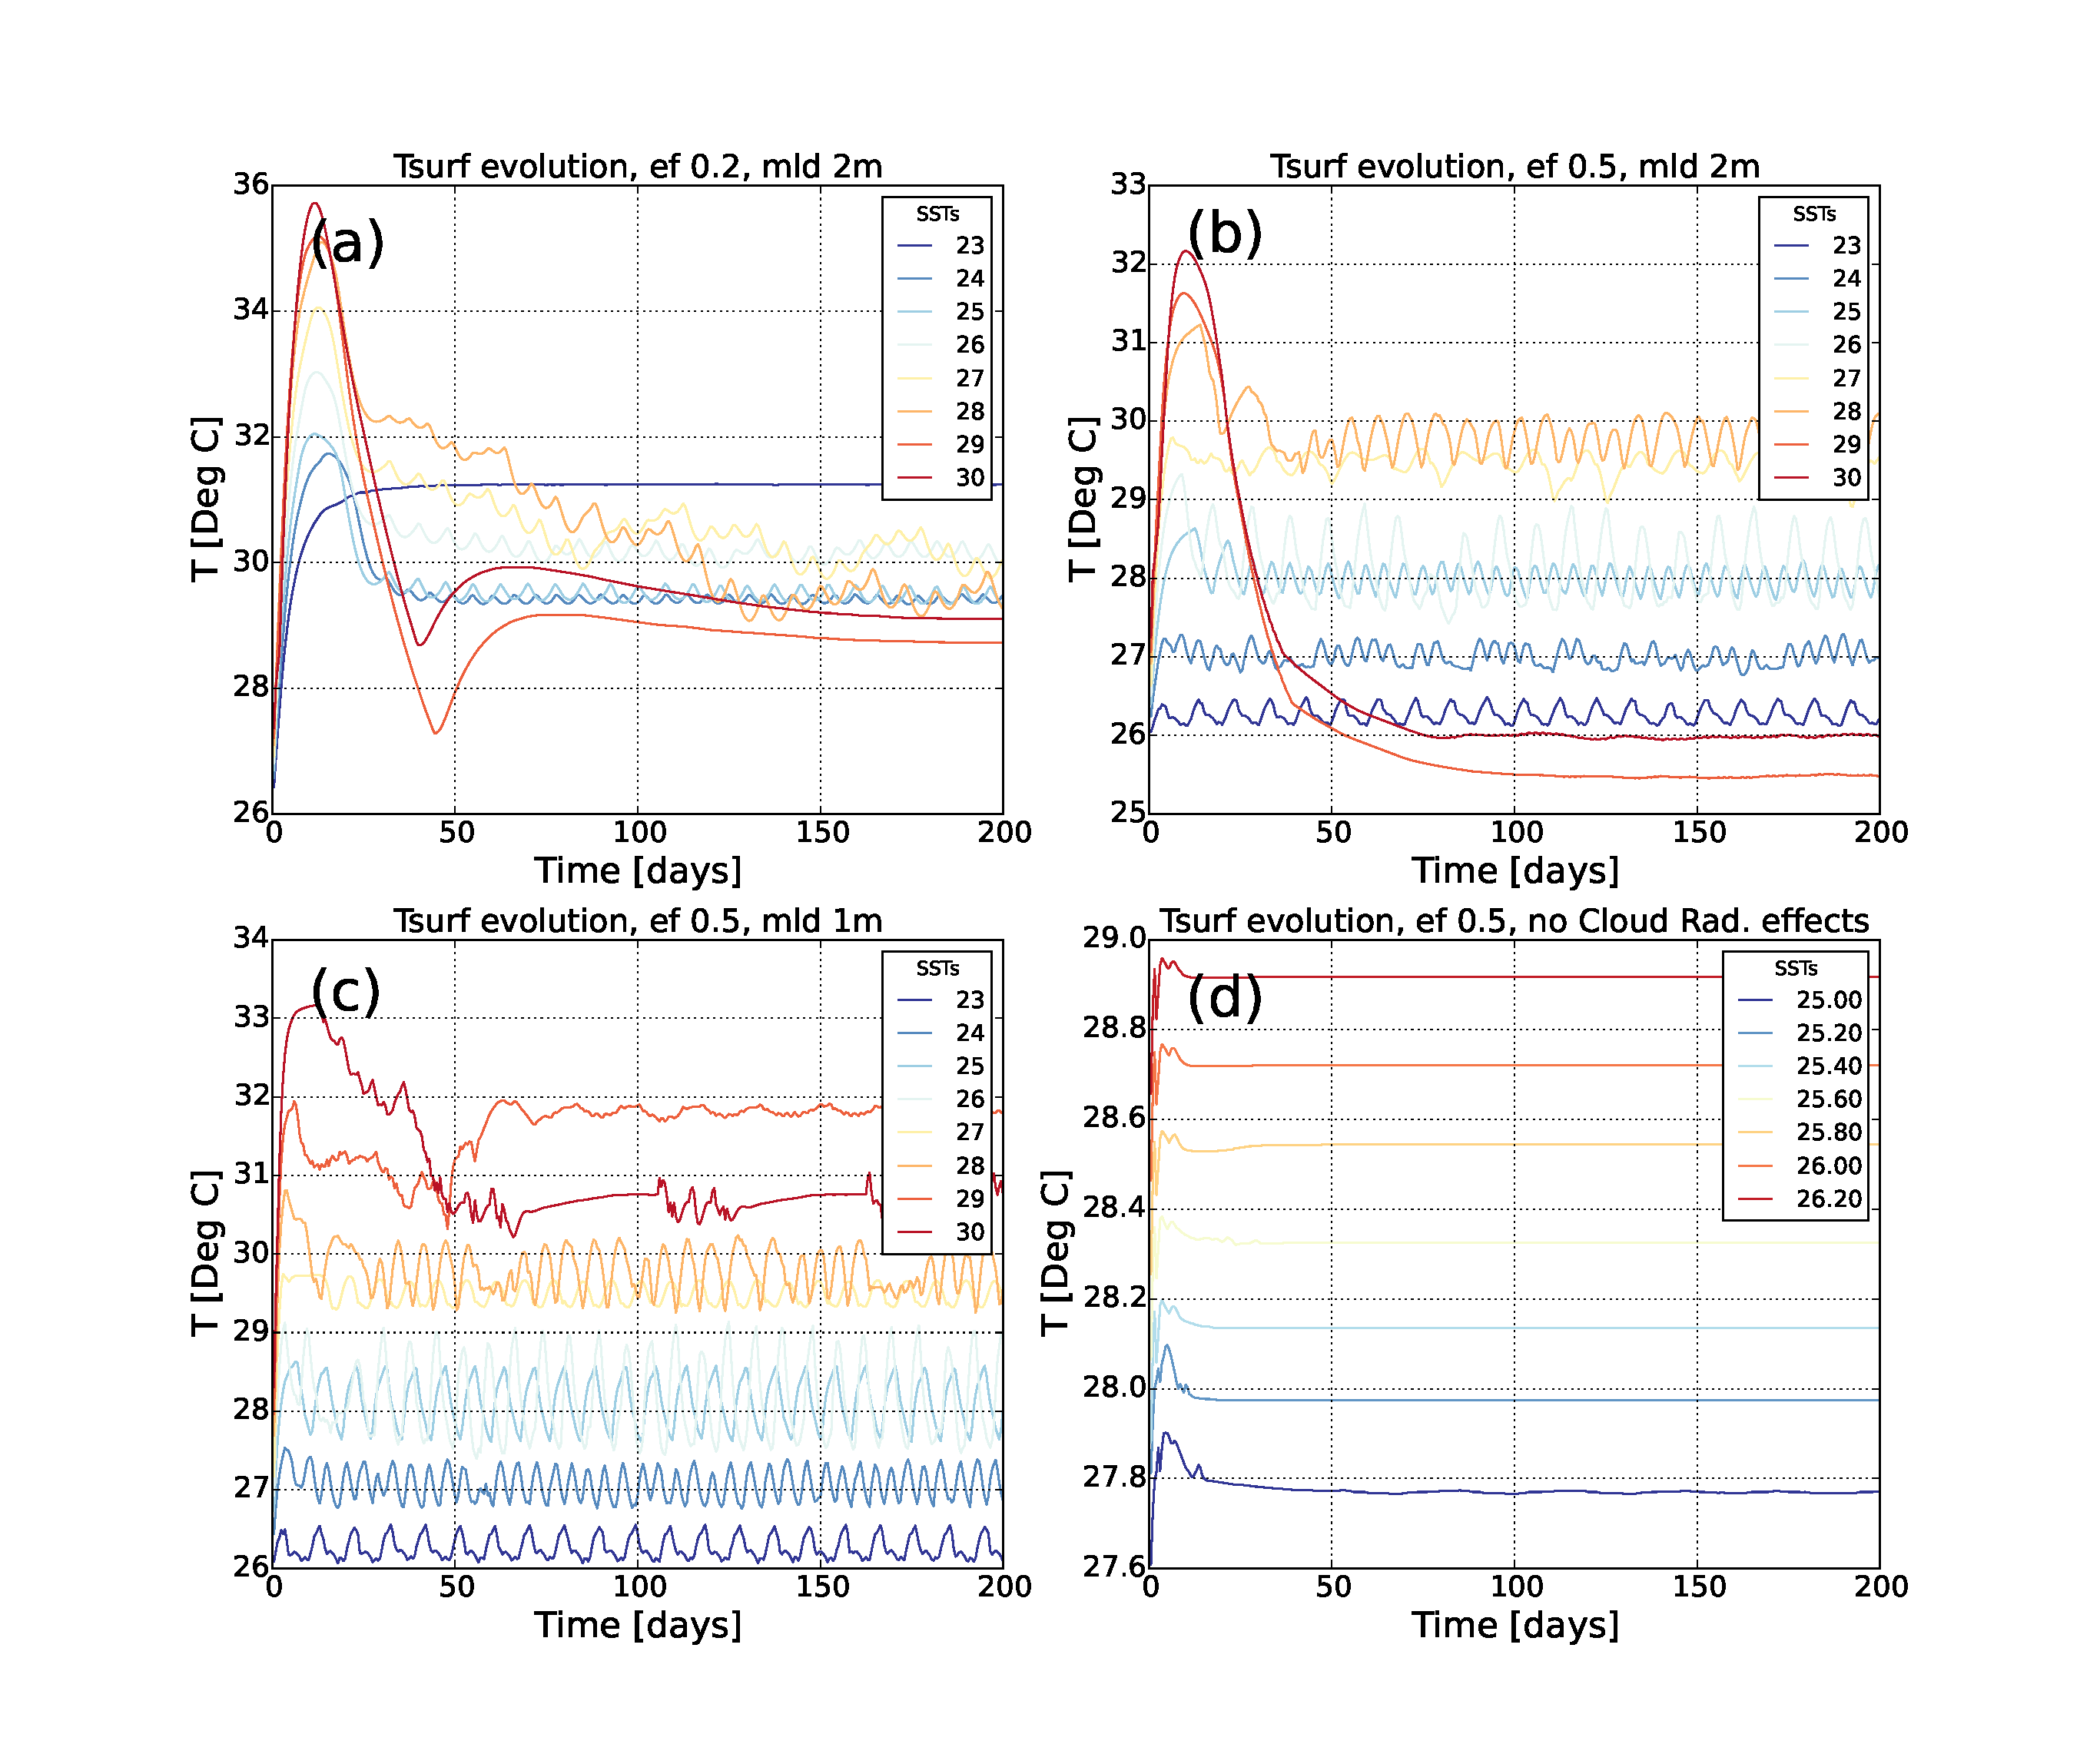
\includegraphics[width=1.0\textwidth]{thesis_instab_Tsurf.eps}
% \includegraphics[width=0.4\textwidth]{land_Tsurf_05_m2_h850.eps}\\
% \includegraphics[width=0.4\textwidth]{land_Tsurf_02_m2_h850.eps}
% \includegraphics[width=0.4\textwidth]{land_nir_Tsurf.eps}\\
\caption{Timeseries of $T_{surf}$ in SCM forced with tropospheric temperature 
profile. a), b) and c) all have the interaction between the convection and 
radiation schemes turned on, it is turned off for d). a) and b) only vary in the 
mixed layer depth of the surface, a) and c) vary in the evaporative fraction.}
\label{fig:scmts}
\end{figure}

\clearpage

\section{Zonally aligned rows of ocean and land columns}
\label{mech_mcm}

The single column model in weak temperature gradient mode offered a promising 
and novel approach to investigating the land/ocean contrast and the role of 
ocean forcing.  However, a few issues remained; the instability of the model 
under certain conditions has the potential to lead to unrealistic results, and 
disabling the interaction between the convection and radiation schemes damped  
the land response. In addition, the assumptions of the WTG approximation are 
only valid in the tropics, a limiting factor when attempting to explain the 
regional differences in the land response. In order to continue using the column 
model while avoiding these issues a multi column setup was used. Multiple 
columns can be coupled to each other in a zonal or meridional direction. In this 
section we primarily use a zonal alignment, a meridional alignment is discussed 
in section \ref{mech_compare}.\\
In the single-column model tropospheric profiles were generated with a range of 
SSTs in an ocean forced column, then used to force the free troposphere of a land 
column. For the zonal and meridional column rows the model is forced directly 
with SSTs in the ocean forced columns, and the troposphere and land surface responds to 
that. 

\subsection{Robust values of land/ocean contrast with varying model geometries}

The column model can be run with one or more ocean and one or more land columns 
in a zonal or meridional alignment. In the single-column model the interaction 
between clouds and radiation lead to instabilities, yet disabling the 
interaction caused a damping of the ocean signal over land and $R_{l/o}$ values 
near to unity. The cloud/radiation interaction was switched off when running the 
model as rows of ocean and land columns and in contrast to a single-column in 
WTG mode, in the multi column model imposed SSTs still lead to an amplified 
response over land. Overall the values of $R_{l/o}$ are lower than the single 
column model but they also show an robust increase $R_{l/o}$ with decreasing 
evaporative fraction.   

A number of different geometries of land and ocean columns were tested, with the 
resultant $R_{l/o}$ values shown in Table \ref{tab:tdm_Rlo}. The values of 
$R_{l/o}$ were largely insensitive to the number of either ocean or land 
columns, although a single ocean and single land column did produce a slightly 
higher $R_{l/o}$. As with the single-column a drier surface increases the 
amplification of the ocean signal over land. However the breakdown of $R_{l/o}$ 
into correlations and ratio of standard deviations we see a difference. The 
correlation values are all very close to one.


\begin{center}
	\begin{table}[ht]
		\caption{Land/Ocean contrast in two dimensional model}
		\label{tab:tdm_Rlo}
		\scriptsize
	\begin{tabular}{ l  c  c  c  c  c }
		\hline
		\textit{Evap Fraction}	& 0.05  & 0.10 & 0.30  & 0.50  & 0.70 \\ \hline
		\textbf{1 Ocean, 1 Land}\\
		$R_{l/o}$ 					& 1.28  & 1.23 & 1.03  & 1.05 & 1.00\\ 
		Corr.					& 0.98  & 1.00 & 1.00  & 1.00 & 1.00\\ %\hline
		Ratio STD          		& 1.30  & 1.23 & 1.03  & 1.05 & 1.00\\ \hline
		\textbf{3 Ocean, 1 Land}\\
		$R_{l/o}$ 					& 1.17  & 1.12 & 1.03  & 1.01 & 0.98\\ %\hline
		Corr.					& 1.00  & 1.00 & 1.00  & 1.00 & 1.00\\ %\hline
		Ratio STD          		& 1.17  & 1.12 & 1.03  & 1.01 & 0.98\\ \hline
		\textbf{1 Ocean, 3 Land}\\
		$R_{l/o}$ 					& 1.13  & 1.10 & 1.02  & 0.94 & 0.86\\ %\hline
		Corr.					& 1.00  & 1.00 & 1.00  & 1.00 & 1.00\\ %\hline
		Ratio STD          		& 1.13  & 1.10 & 1.02  & 0.94 & 0.86\\ \hline
		\textbf{3 Ocean, 3 Land}\\
		$R_{l/o}$ 					& 1.16  & 1.11 & 1.00  & 0.96 & 0.91\\ %\hline
		Corr.					& 1.00  & 1.00 & 1.00  & 1.00 & 1.00\\ %\hline
		Ratio STD          		& 1.16  & 1.11 & 1.00  & 0.96 & 0.91\\ \hline
	\end{tabular}
	\end{table}
\end{center}

\subsection{Vertical structure and tropospheric response over land and ocean in 
the column model}

The single and multi column model was used with the purpose of understanding the 
vertical structure of the land/ocean temperature contrast. We can see from Table 
\ref{tab:tdm_Rlo} that when using small evaporative fractions we can reproduce 
the magnitude of $R_{l/o}$ seen in GCMs and observation. We will now compare the 
vertical structure and response of the column model with a GCM, specifically 
with results from the ENSO-Pacemaker experiments.  

Figure \ref{fig:tdm_regprof} uses the same technique as in Figure 
\ref{fig:linreg_plev}; the blue line is the regression coefficient between the 
temperature at each model level in the ocean forced column and the SSTs, the green line 
is the regression coefficient between the temperature at each model level in the 
land column and the SSTs. Figures \ref{fig:tdm_regprof} a) -- the multi column 
model and b) -- the GCM, have some key similarities and differences; the ocean 
profiles are both very similar, they feature the large amplification around 
\SIrange{200}{400}{\hecto\pascal} due to moist convection, as well as a local 
maximum at the freezing level at \SI{600}{\hecto\pascal}.  Comparing the 
profiles above land we see a large difference above \SI{500}{\hecto\pascal}. In 
the GCM the moist convective amplification is communicated above land areas but 
becomes damped whereas in the column model the two profiles follow each other 
closely.  This doesn't necessarily imply the presence of moist convection in the 
land columns, merely that the land and ocean are more tightly linked in the 
multi column model.  Allowing for this discrepancy the GCM and column model are 
very similar.  In the area above \SI{800}{\hecto\pascal} the land/ocean contrast 
disappears and below \SI{800}{\hecto\pascal} the land and ocean profiles diverge 
to give similar values of $R_{l/o}$.\\
From Figure \ref{fig:tdm_regprof} we can assume that there may be difference in 
the land surface response in the GCM and multi column model due to the 
discrepancy in the upper troposphere response, but importantly the lower 
atmospheric response is very similar, making the simplified model suitable for 
further investigation of the land/ocean temperature contrast and the role of 
ocean forcing.


\begin{figure}[ht]
	\includegraphics[width=0.5\textwidth]{{thesis_fsstreg_prof_ocensfc_e0.05}.eps}
	\includegraphics[width=0.5\textwidth]{{thesis_linreg_ocean_profile}.eps}
	\caption{Linear regression coefficients for temperature above tropical ocean 
		(blue line) and land (green line) as linear model of $T_{ocean}$ for the 
	two dimensional column model (a) and the ENSO-Pacemaker experiment (b).}
\label{fig:tdm_regprof}
\end{figure}


\subsection{Atmospheric profiles of temperature and relative humidity}

In section \ref{scm_prof} the atmospheric profiles of $\theta$ for the single 
column indicated that a changing LCL height over land as well as a deviation 
between land and ocean lapse rates above the LCL can lead to $R_{l/o}>1$. We 
will know look at profiles of $\theta$ in the multi column model. The potential 
importance of a changing LCL height motivated an increase in the vertical 
resolution of the model.  The grid was non-uniform with 85 levels, and a 
resolution of \SI{5}{\hecto\pascal} between \SIrange{980}{800}{\hecto\pascal} 
and \SI{10}{\hecto\pascal} between \SIrange{800}{650}{\hecto\pascal}, with the 
fine resolution preventing step changes in the height of the LCL.  Figure 
\ref{fig:tdm_prof} shows three temperature profiles from a run with an 
evaporative fraction of 0.05 and an $R_{l/o}$ of 1.13. The three profiles are 
the maximum, minimum and median SST forcing. The full profile is shown in (a) 
with a close up in (b). There are two features to look for; a change in the 
gradient of $\theta$ in the ocean forced column between the ocean LCL and land LCL as 
per the \citet{Byrne2013a} theory, and any significant change in the height of 
the LCL as seen in the single column model. There is some indication in the 
figure of a small change in the LCL over land and ocean but a change in gradient 
is difficult to determine.  Figure \ref{fig:tdm_dthdp} shows the vertical 
gradient of $\theta$, $D\theta/Dp$, to determine any significant features.  An 
increase in the magnitude of $D\theta/Dp$ (i.e. more negative) would indicate a 
flatter profile, and the height of the local minimum can indicates the location 
of the LCL. In Figure \ref{fig:tdm_dthdp}, the gradient of $\theta$ in the ocean 
column above the LCL becomes more negative with increasing SST which is the 
expected result according to the Byrne and O'Gorman theory.  However, there is 
also an unusual feature; from \SIrange{900}{800}{\hecto\pascal} the land profile 
is above, or cooler than, the ocean profile. This region of warmer ocean/cooler 
land could have the effect of dampening the value of $R_{l/o}$ and is not an 
expected feature.  To understand what is happening we will look at the profiles 
of relative humidity

\begin{figure}[ht]
	\includegraphics[width=0.5\textwidth]{{thesis_l3o1_prof_theta_ef0.05}.eps}
	\includegraphics[width=0.5\textwidth]{{thesis_l3o1_prof_theta_ef0.05_close}.eps}
	\caption{Atmospheric profiles of theta in the multi model for forcing SST 
	values of \SI{24}{\degreeCelsius}, \SI{26}{\degreeCelsius and 
\SI{28}{\degreeCelsius}}}
\label{fig:tdm_prof}
\end{figure}

\begin{figure}[ht]
	\includegraphics[width=0.5\textwidth]{{thesis_l3o1_prof_dthetadp_ef0.05_close}.eps}
	\caption{Profiles of $D\theta/Dp$ in the multi model in the land (solid) and 
	ocean (dashed) columns, showing the decrease in gradient (more negative) in 
the ocean forced column with warmer SST values} \label{fig:tdm_dthdp}
\end{figure}

Regarding the warmer ocean/cooler land profile from 
\SIrange{980}{800}{\hecto\pascal}, the profiles of relative humidity are quite 
telling. The relative humidity profile in Figure \ref{fig:tdm_rhprof} a) is from 
the same run as Figure \ref{fig:tdm_prof}, it has one ocean and three land 
columns. Two SSTs are plotted, the warmest and coolest of the runs, as the 
results are similar for a range of SSTs.  From the surface we see the much 
higher relative humidity over the ocean forced column then a sudden drop at around 
\SI{970}{\hecto\pascal}, to the extent that the ocean forced column becomes drier than 
the land columns. The dry region, from \SIrange{940}{800}{\hecto\pascal} 
coincides with the steeper $\theta$ lapse rate. As this run only has one ocean 
column and three land columns the region may be related to the model geometry.  
To test if the geometry is responsible for the dry region, we look at a run with 
three ocean and three land columns.  Figures \ref{fig:tdm_rhprof} (b)-(d) all 
show a similar drying in the ocean forced column, these are also focusing on the 
atmosphere below \SI{800}{\hecto\pascal}. There is a robust response with the 
three ocean and three lands, implying the drying is not a function of the 
geometry.  Figures \ref{fig:tdm_rhprof} (b), (c) and (d) show three difference
evaporative fractions, 0.05, 0.10 and 0.20. The evaporative fraction has a clear 
effect on the relative humidity in the land column, but the amount of drying in 
the ocean forced columns is largely insensitive to the evaporative fraction or relative 
humidity of the land columns. For example comparing Figure \ref{fig:tdm_rhprof} 
b), c) and d) which have evaporative fractions of 0.05, 0.10 and 0.20  
respectively, the near surface humidity in the land columns changes from 45\% to 
60\%, however the response of the ocean forced columns is very similar.  The difference 
in the dry region is at most 5\%.
To summarise, the atmospheric profiles of $\theta$ indicate the possibility that 
a change in the $\Gamma_m^*$ between the land and ocean LCL heights, as per 
\citet{Byrne2013a}, could contribute to the land/ocean contrast. However the 
lapse rate over the ocean is being affected by a strong drying from the land 
column, indicated in the relative humidity profiles. We will look at the 
circulation response in the model to further explore this.

\begin{figure}[ht]
	\includegraphics[width=0.5\textwidth]{{thesis_l3o3_prof_rh_ef0.05}.eps}
	\includegraphics[width=0.5\textwidth]{{thesis_l3o3_prof_rh_ef0.05_close}.eps}
	\includegraphics[width=0.5\textwidth]{{thesis_l3o3_prof_rh_ef0.10_close}.eps}
	\includegraphics[width=0.5\textwidth]{{thesis_l3o3_prof_rh_ef0.20_close}.eps}
	\caption{Atmospheric profiles of relative humidity in the multi column model, a) has 
		one ocean and three land columns, b)-d) have three ocean and land 
		columns (mean values shown), land surface has evaporative fractions of 
	0.05 (a), 0.05 (b), 0.10 (c) and 0.20 (d).}
\label{fig:tdm_rhprof}
\end{figure}

\subsection{Circulation response in a row of columns}
To see what is causing the drying in the ocean forced columns we look at the 
vertical velocity, $\omega$ and circulation using the streamfunction $\psi$ of 
vertical and zonal velocities. There weren't any significant changes in the 
circulation for varying SSTs so for these variables we use the mean across a 
range of SSTs.  The profiles of $\omega$ clearly shows the convection in the 
ocean forced columns -- positive values of $\omega$ -- which are balanced with 
sinking motion in the land columns.  The $\psi$ profile better demonstrates the 
flow in the model, and shows a low level circulation response. Positive values 
of $\psi$ indicate clockwise flow centered at \SI{850}{\hecto\pascal} in the 
ocean forced column nearest the land.  This circulation is responsible for 
transporting dry air from the land columns.

\begin{figure}[ht]
	\includegraphics[width=0.5\textwidth]{{thesis_l3o3_omegal_ef0.05_meansst}.eps}
	\caption{Circulation response in the multi column model, a) Omega (vertical 
	velocity).}
	\label{fig:tdm_circ}
\end{figure}

This circulation is influencing the atmospheric structure in the ocean forced 
column, but is it affecting the ocean's influence of the land column, and thus 
the value of $R_{l/o}$? This drying of the atmosphere above the ocean is not 
present in a large scale across the globe and therefore could be of concern when 
determining the suitability of this simplified model when comparing the results 
to GCMs or observations.  Figure \ref{fig:tdm_psi} (a)-(d) shows how the low 
level circulation scales with evaporative fraction. A drier land surface results 
in a  stronger low level circulation.  Referring back to Table 
\ref{tab:tdm_Rlo}, $R_{l/o}$ increases with decreasing evaporative fraction. If 
the value of $R_{l/o}$ is related to the difference in lapse rates above land 
and ocean, which in turn is related to the difference in humidity, then a drying 
of the ocean forced column may lead to a smaller difference between the ocean 
and land columns.  Instead, we see that the magnitude of the reduction in 
humidity in the ocean forced columns is largely insensitive to the evaporative 
fraction (Figure \ref{fig:tdm_rhprof}) and while the strength of the low level 
circulation driving the reduced humidity increases with evaporative fraction, 
the value of $R_{l/o}$ still increases, implying that the drying of the ocean 
forced column is not significantly affecting the value of $R_{l/o}$, or more 
importantly, the ability of the simplified model to simulate the land/ocean 
contrast.

\begin{figure}[ht]
	\includegraphics[width=0.5\textwidth]{{thesis_l85co2_psi_ef0.05_mean}.eps}
	\includegraphics[width=0.5\textwidth]{{thesis_l85co2_psi_ef0.10_mean}.eps}
	\includegraphics[width=0.5\textwidth]{{thesis_l85co2_psi_ef0.20_mean}.eps}
	\includegraphics[width=0.5\textwidth]{{thesis_l85co2_psi_ef0.30_mean}.eps}
	\caption{Circulation response for the multi column model, Psi, for 
	evaporative fractions on 0.05, 0.10, 0.20, 0.30. The low-level circulation 
centred at \SI{850}{\hecto\pascal} strengthens as the evaporative fraction 
decreases.}
	\label{fig:tdm_psi}
\end{figure}

\clearpage

\subsection{Values of land ocean contrast for different evaporative fractions 
and latitudes}

We have seen that while the two-dimensional model has a low level circulation 
that dries the ocean forced column, it is still able to simulate aspects of the 
land/ocean contrast we see in GCMs (i.e. Figure \ref{fig:tdm_regprof}), and it's 
response to surface properties is expected from the lapse rate of theories of 
\cite{Joshi2007} and \cite{Byrne2013a}. We now extend the range of evaporative 
fractions and vary the latitudes to build a picture of the range of $R_{l/o}$ 
values.\\
The model had 3 ocean and 3 land columns and initially was run in a zonally 
orientated domain. At each latitude an appropriate mean SST value, solar zenith 
angle and Coriolis parameter were used.  The model was forced with a range of 
SSTs values which varied around the mean value for each latitude, and $R_{l/o}$ 
was calculated for each parameter.	The results, in Figure \ref{fig:tdm_Rlo} 
show the dependence of $R_{l/o}$ on evaporative fraction, but also a decrease 
with latitude, excepting the increase from \SI{0}{\degree} and \SI{10}{\degree}.  
The same experiments were also performed using a meridionally orientated domain, 
where the prescribed SST columns were nearer to the ``equator" and the land 
columns extended towards the poles.  In the meridional domain the values of 
$R_{l/o}$ show the same tendencies as in the zonal domain, but at first appear 
lower than the zonal domain. However, as each column spans \SI{5}{\degree} of 
latitude, if we take the $R_{l/o}$ values of a specific column and compare it to 
the corresponding latitude of the zonally orientated model we see they are quite 
similar, i.e. Figure \ref{fig:tdm_Rlo} (d). When looking at the nearest 
corresponding latitudes in (a) and (d), e.g. \SI{40}{\degree} in (a) and 
\SI{45}{\degree} in (d) the values of $R_{l/o}$ are very similar.  The reduction 
in the $R_{l/o}$ with increasing latitude could be due to reduced transport 
across the domain. The latter is evident in Figure \ref{fig:tdm_Rlo} c), which 
shows the mean relative humidity in the land columns. The gradient of relative 
humidity along a constant latitude due to varying evaporative fraction is clear, 
and increasing relative humidity corresponds to decreasing $R_{l/o}$ as 
expected.  The relative humidity also decreases with increasing latitude, due to 
reduced transport of moisture from the ocean forced columns, further discussed 
below.  For the gradient of relative humidity across latitudes, decreasing 
relative humidity is associated with decreasing $R_{l/o}$, the inverse of the 
relationship with a constant latitude.  This indicates that the value of 
$R_{l/o}$ is a not only a function of evaporative fraction but is also dependent 
on transport from ocean forced columns to land columns.\\

\begin{figure}[ht]
	\includegraphics[width=0.5\textwidth]{{isstcosz}.eps}
	\includegraphics[width=0.5\textwidth]{{coszmer_colall}.eps}\\
	\includegraphics[width=0.5\textwidth]{{latbox_landrh}.eps}
	\includegraphics[width=0.5\textwidth]{{coszmer_col1}.eps}
	\caption{Land/ocean contrast ($R_{l/o}$) in multi column model for a range 
		of evaporative fractions and latitudes for a zonally aligned domain (a), 
		meridionally aligned domain (b). (c) is the mean (over the forcing SSTs) 
	relative humidity at each latitude and evaporative fraction, (d) uses the 
first column of the meridionally aligned model to calculate $R_{l/o}$ instead of 
the areal mean across all columns.}
\label{fig:tdm_Rlo}
\end{figure}

\section{Comparison of Simplified Models and GCM results}
\label{mech_compare}

The large range of $R_{l/o}$ values allows for a direct comparison to GCM 
results. Using the pacemaker experiment we can calculate an $R_{l/o}$ value for 
each individual land grid box, see Figure \ref{fig:tdm_gcm_compare} a). We do 
this by comparing the grid box surface temperature of with either the mean 
tropical SSTs, mean global SSTs or zonally averages SSTs corresponding to the 
latitude of the grid box. The latter may seem most appropriate for comparing to 
the zonally orientated multi column model, however the tropical Pacific forcing 
of the pacemaker experiment meant that a grid box $R_{l/o}$ calculated using 
mean tropical SSTs gave the most reasonable results.\\
The next step is to generate a comparative map using the multi column column model 
results. For each GCM grid box we find the latitude and evaporative fraction, 
then we take the $R_{l/o}$ from the multi column model run with corresponding parameters, 
see Figure \ref{fig:tdm_gcm_compare} b).  For example, for a point in central 
Australia at a latitude of \SI{23}{\degree} and evaporative fraction of 0.2 we 
use the $R_{l/o}$ from the multi column model at latitude \SI{20}{\degree} and evaporative 
fraction 0.2 and assign that grid box a value of 1.12, thereby building a global 
map of the expected land surface temperature response based on the results of 
the two dimensional column model.\\
The two-dimensional model required very low evaporative fractions to elicit an 
$R_{l/o}>1$, lower than would be required from a GCM or expected from 
observations. As such we wouldn't expect the magnitudes the generated $R_{l/o}$ 
response map to perfectly match a similar GCM map. However, if the multi column model was 
capturing a significant mechanism of the land/ocean temperature contrast, that 
is, the oceans control the tropospheric temperature and the drier land surface 
affects the mean lapse rate, then we might expect the broad patterns to be 
similar between the multi column model and GCM results. It is clear that the two plots in 
Figure \ref{fig:tdm_gcm_compare} share little resemblance in magnitude or 
patterns.\\
The only two large regions of the generated map with an $R_{l/o}>1$ are Saharan 
Africa and central Australia, and yet in both these regions the pattern of the 
land response differs from the GCM. For example, in Saharan Africa the generated 
map shows a very consistent $R_{l/o}$ from western coast of Africa to the 
Persian gulf, as this region is of a similar dryness. In contrast, the GCM 
results only have an $R_{l/o}>1$ for the western half of the region. Likewise in 
south-eastern Australia the GCM has a higher $R_{l/o}$ whereas the multi column model has 
lower values for that region. Another area of interest is tropical South 
America, here the GCM has high $R_{l/o}$ values and a distinctive pattern with a 
very high "blob" over the Amazon basin, none of which is present in the multi column 
model.\\
This result may be seen as an indication that the simplified radiative 
convective model is inadequate in modelling the land/ocean contrast, but the 
model does capture some theoretical aspects as expected. Therefore if we 
consider the differences between the two maps in Figure 
\ref{fig:tdm_gcm_compare} as indicative of the processes missing from the simple 
model, we can use this as a guide to understanding the regional response of the 
land surface to an ocean forcing.

\clearpage

\begin{figure}[ht]
	\includegraphics[width=0.9\textwidth]{{phi_trop_4ysl}.png}\\
	\includegraphics[width=0.9\textwidth]{{phi_rcm_4ysl}.png}
	\caption{a) Values of $R_{l/o}$ for the ENSO-Pacemaker experiment calculated 
	for each grid box and using mean tropical SSTs, b) $R_{l/o}$ taken from the 
multi column model and matched to the latitude and evaporative fraction of the GCM.}
\label{fig:tdm_gcm_compare}
\end{figure}

An obvious process missing from the multi column model results in Figure 
\ref{fig:tdm_gcm_compare} is the interaction between clouds and radiation. This 
can lead to chaotic results but clearly might still be important. The plot from 
Figure \ref{fig:tdm_Rlo} was repeated but with the interaction between clouds 
and radiation turned on. The plot in Figure \ref{fig:tdm_Rlo_ic} is broadly 
similar in terms of the evaporative fraction, in that a drier surface tends to 
have a higher $R_{l/o}$.  The tendency of $R_{l/o}$ with latitude is different, 
we don't see a reduction with increasing latitude.  The main feature, however, 
is the randomness present in the results.  It seems at certain latitudes the 
model behaves strangely, namely at \SI{10}{\degree} where values are very low 
and \SI{40}{\degree} where they are very high. It is clear that a map created 
using these results would contain inconsistencies.

\begin{figure}[ht]
	\includegraphics[width=0.6\textwidth]{{isstcosz_ic}.eps}
	\caption{Land/ocean contrast ($R_{l/o}$) in multi column model for a range of 
	evaporative fractions and latitudes for a zonally aligned domain, same as 
Figure \ref{fig:tdm_Rlo} a) except with the interaction between clouds and 
radiation turned on.}
\label{fig:tdm_Rlo_ic}
\end{figure}

In Figure \ref{fig:tdm_Rlo} c) we saw that relative humidity decreased with 
increasing latitude, and this was associated with a decreasing $R_{l/o}$. It was 
theorized that the reduction in relative humidity coincided with decreased 
transport from the ocean to the land columns, which then resulted in a lower 
$R_{l/o}$. We will now look at the circulation response with latitude to 
understand the changes. As the latitude increases there is clear change in the 
circulation. At low latitudes the model is essentially one cell, with rising air 
over the ocean forced columns and sinking over the land. This begins to break 
down at \SI{20}{\degree} and by \SI{30}{\degree} smaller cells have formed 
between each column. This will reduce the transport of heat and moisture from 
the ocean forced columns to the land columns, resulting in the reduced relative 
humidity and reduced values of $R_{l/o}$ seen with increasing latitude.

\clearpage

\begin{figure}[ht]
	\includegraphics[width=0.3\textwidth]{{psi_lats_0.0}.eps}
	\includegraphics[width=0.3\textwidth]{{psi_lats_10.0}.eps}
	\includegraphics[width=0.3\textwidth]{{psi_lats_20.0}.eps}\\
	\includegraphics[width=0.3\textwidth]{{psi_lats_30.0}.eps}
	\includegraphics[width=0.3\textwidth]{{psi_lats_40.0}.eps}
	\includegraphics[width=0.3\textwidth]{{psi_lats_50.0}.eps}\\
	\caption{circulation response, psi, with changing latitude.}
	\label{fig:tdm_psi_lat}
\end{figure}


\newpage

%----------------------------------------------------------------------------------------
%	Regional Response / GREB
%----------------------------------------------------------------------------------------

\section{Mechanisms of the Regional Response}
\label{mech_greb}

In our investigations with the single column and multi column models we found 
that the modelled land/ocean contrast compared well to the mean global and 
tropical values from observations and GCMs in terms of both the statistics and 
the vertical structure. In the column model there was a robust dependancy of the 
value of $R_{l/o}$ on the dryness of the land surface, which is controlled 
through the evaporative fraction. The value of $R_{l/o}$ in the multi column 
model also had a dependence on latitude. When the column model results were 
compared to regional values from a GCM there were large discrepancies.  While 
the dryness of the surface certainly contributes to the land/ocean contrast in 
the GCM results, it does not control the magnitude of the regional response. 
There are many continental regions where SST signals become amplified that 
cannot be explained by the column model.

In this section we are going to continue to investigate the land/ocean contrast 
by focusing on the regional response of land to an ocean forcing. We define the 
regional scale as continental to sub-continental, with different regions loosely 
defined by a pattern or similarity of response in a certain area. To investigate 
this regional response we use the Globally Resolved Energy Balance model (GREB 
model)  to recreate the patterns of temperature response seen in the 
ENSO-Pacemaker experiments.  

\subsection{GREB Model - Deconstructing the regional response}

The GREB model and the ENSO-Pacemaker experiments were chosen for a few specific 
attributes. In the GREB model the prognostic variables are the surface 
temperature, atmospheric temperature, upper ocean temperature and atmospheric 
water vapour, all calculated on a global grid \citep{Dommenget2011}. The aspect 
of the GREB model that is most useful for this work is that the boundary 
conditions include meridional and zonal winds, surface wetness fraction, and 
cloud cover.  The ocean surface temperature can either be assigned, or a 
responsive slab ocean can be used.  Starting with climatological values, 
anomalies can be added to these variables to recreate, for example, the 
atmospheric conditions during the time of the peak land response to an ocean 
forcing. In addition, the anomalies can be added to one variable individually, 
or in any combination to build a picture of the response, and determine the 
important factors for each region.

We have a versatile, globally resolved model that we can use to build a picture 
of the regional response of land surface, but we need a suitable way to force 
the model. For this, we used the ENSO-Pacemaker experiments. The regular and 
repetitive forcing in the ENSO-Pacemaker experiment allows for composites to be 
easily made for the period of maximum and minimum land response.  As we are 
interested in the land surface response, the composites consist of six months of 
the maximum (or minimum) response over land. The land response is delayed by 
around 3 months from the peak ocean forcing (as outlined in section \ref{xcor}) 
so the composite is the mean of months 0 to 6 after the peak ocean forcing in 
the Pacific Ocean. 

The GREB model experimental setup for this section has three key parts; a) 
Composites of anomalies of soil moisture, SSTs, meridional winds, zonal winds, 
and cloud cover are created from the ENSO-Pacemaker experiments, using months 0 
to 6 after the peak forcing.  A composite of land surface temperature is also 
generated to compare to the GREB results, b) The anomalies from these composites 
are applied to the climatological boundary conditions in the GREB model.  
Anomalies for each of the variables listed above are added individually then in 
combination, and for each anomaly or combination of anomalies the GREB model is 
run to equilibrium, c) The surface temperatures from each GREB equilibrium run 
are compared against the composite surface temperature from the ENSO-Pacemaker 
run, in order to determine which variables are the important on regional or 
global scales.

\subsubsection{Composite temperature response from the ENSO-Pacemaker 
experiment}

Before investigating the experiments with the GREB model we will look at the 
surface temperature response in the ENSO-Pacemaker experiment, essentially, the 
response we wish to recreate with the GREB model.  Figure \ref{fig:comp_temp} 
are the composites of months 0 to 6 after the maximum warming (a) and maximum 
cooling (b) of the Pacific Ocean forcing. The colour-bar for the cooling is 
reversed to allow comparison of the two figures. Both the response patterns and 
the magnitude of warming and cooling are similar, implying the response is 
fairly linear, although in some regions the warming forcing warms more than the 
cooling forcing cools.  The area with the greatest discrepancy and a difference 
in the sign of the surface temperature response are the high northern latitudes 
of Europe and Asia, which is also the region most removed from the area of 
forcing.  Other features true to both plots include a positive (i.e.  warming or 
cooling in same direction as forcing) response in tropical South America, with a 
strong amplification in the Amazon basin, a distinctive pattern across Africa, 
with a positive response everywhere except the north eastern region. High 
latitude North America has a strongly amplified positive response in both plots.  
The negative responses in the subtropical regions of South America and north 
eastern Africa are similar but weaker in the cooling scenario. Overall we see a 
positive response over most land surfaces, with some specific patterns of 
negative response, and some areas show a significantly increased amplification 
to the ocean forcing.

\begin{figure}[ht]
\includegraphics[width=0.5\textwidth]{{comp_Tmax_sfc}.eps}
\includegraphics[width=0.5\textwidth]{{comp_Tmin_sfc}.eps}
\caption{ENSO-Pacemaker surface temperature for composite of months 0 to 6 after 
peak forcing. Positive forcing on left (a), negative on right (b).}
\label{fig:comp_temp}
\end{figure}

\subsubsection{Composite anomalies from the ENSO-Pacemaker experiment}

Figure \ref{fig:comp_5var} shows the composite anomalies from the ENSO-Pacemaker 
experiments which will be used as boundary conditions in the GREB model. These 
are the composites for the maximum positive forcing resulting from a warming in 
the tropical Pacific Ocean. 

In Figure \ref{fig:comp_5var} (a) the cloud cover anomalies show a large 
increase in cloud cover above the forcing region in the tropical Pacific, as the 
heating from the ocean leads to convective clouds.  This is matched with a 
decrease in cloud north and south in the subtropics, and also the to east and 
west, above tropical South America and the Maritime continent. The surface 
wetness fraction response, although weak, corresponds to the cloud cover 
response in most regions, with reduced cloud cover leading to drying (negative 
values) and increased cloud cover leading to moistening (positive values). This 
is seen most clearly in South America, where drying in the Amazon basin 
corresponds to reduced cloud, and moistening around \SI{30}{\degree} south is 
associated with increased cloud cover. However the opposite is seen in North 
America, where an increase in soil moisture is associated with a decrease in 
cloud cover. 

The meridional wind anomalies, in Figure \ref{fig:comp_5var} (b), show distinct 
wave patterns in the extra-tropics and high latitudes, indicated by alternating 
positive (southerly) and negative (northerly) anomalies. Although the dynamics 
of the extra-tropical response is not a focus of this study, the distinctive 
extra-tropical wave pattern concurs with theory on the atmospheric response to a 
tropical heat source (e.g. \citealt{Hoskins1981}, \citealt{Sardeshmukh1988}, 
\citealt{Held1989}).  There is convergence in the tropical Pacific, with northerly 
anomalies to the north of the forcing region and southerly anomalies to the 
south. The largest response is in the north-eastern Pacific Ocean, with a strong 
northerly anomaly.  Figure \ref{fig:comp_5var} (d) shows that the zonal wind 
anomalies are strongest in the Pacific Ocean basin, and there is a strong 
positive (westerly) anomaly in the tropical Pacific on the equator, which is 
what would be expected for an El Ni\~no like forcing.  Moving away from the 
equator, there are alternating bands of westerly and easterly wind anomalies.

The tropical Pacific Ocean forcing is clearly seen in the SST anomalies, in 
Figure \ref{fig:comp_5var} (e). Away from the forcing region there is a 
consistent warming throughout the tropics, and a number of regions in the 
mid-latitudes show a cooling response.

To summarise; the composites of winds, clouds, surface wetness fraction and SST all show 
both negative and positive response to the tropical Pacific Ocean forcing, and 
all have large regional differences. In the next section the composite anomalies 
will be used in the GREB model.

\begin{figure}[ht]
\includegraphics[width=1.0\textwidth]{{thesis_anom_input_4ycomp}.eps}
\caption{Anomalous cloud cover (a), meridional (b) and zonal wind (d) surface 
wetness fraction (c) used to force the GREB model.  Generated from 
ENSO-Pacemaker composites.}
\label{fig:comp_5var}
\end{figure}

\begin{figure}[ht]
\includegraphics[width=0.9\textwidth]{{tsurf_clim}.eps}
\caption{Climatological Surface Temperature of GREB model.}
\label{fig:greb_clim}
\end{figure}

\clearpage

\subsubsection{Imposing SST anomalies}

We begin the GREB experiments by looking at the land surface temperature 
response to imposed SSTs, as shown in Figure \ref{fig:greb_sst}. The anomalous 
SSTs field -- the composite from the ENSO-Pacemaker experiment -- is applied to 
the climatological SSTs and the model is run to equilibrium. The SST field 
includes the forcing region in the tropical Pacific and the response of the 
ACCESS slab ocean in the other oceans.  The first thing we note is that the 
amplification of SST signal in the land surface temperatures is not present, as 
it is in the ACCESS model in Figure \ref{fig:comp_temp}, yet the regionality of 
the land response is similar to ACCESS. The majority of warming is in the 
tropical band, following the SST anomalies.  Regarding the lack of amplification 
over land; there are a number of atmospheric processes not present in the GREB 
model which we will explore these further by imposing other anomalous fields, 
but from our previous work we know the importance of the tropospheric structure 
and convection. These are not directly modelled in GREB but are represented 
through an imposed cloud climatology. There are also no changes to the 
circulation, the effect of which we will explore by imposing wind anomalies. So 
we see imposing SST anomalies without  adjusting other factors influencing the 
climate leads to warming over land, but not the amplification we see in ACCESS.

\begin{figure}[ht]
	\includegraphics[width=0.9\textwidth]{{t_surf.sst_anom.pos.4ycomp.response.thesis}.eps}
	\caption{Surface temperature response in GREB to imposed SST anomalies.}
\label{fig:greb_sst}
\end{figure}

\subsubsection{Imposing zonal and meridional winds anomalies}

In Figure \ref{fig:greb_uv} we see the surface temperature response to imposed 
zonal (a), meridional (b) and combined (c), \SI{850}{\hecto\pascal} wind 
anomalies. These runs used climatological values for clouds and surface wetness 
fraction with a responsive slab ocean. The anomalous winds were added to the 
climatological winds and the model was run to equilibrium.  Figure 
\ref{fig:greb_uv} (a) shows the zonal wind anomalies lead to a small but 
consistent warming in many areas, with the only large region of cooling in the 
north west Pacific. There are no clear similarities with the temperature 
response in Figure \ref{fig:comp_temp}.  The surface temperature response to 
meridional wind anomalies in Figure \ref{fig:greb_uv} (b) shows some more 
interesting response patterns. Anomalous poleward winds in the northern Indian 
Ocean and South China Sea increase heat transport to continental Asia, resulting 
in a large warming. Similarly , in the south-eastern Pacific Ocean and the high 
latitudes of North America, anomalous poleward winds lead to warmer 
temperatures. There is warming across much of the tropics, land and ocean, with 
the exception of the western Pacific where there is a large cooling from the 
tropics to both poles.  Most of the temperature response can be explained by 
considering the heat transport of the anomalous winds (i.e. Figure 
\ref{fig:comp_5var} (b)), and the mean surface temperature climatology of the 
model, Figure \ref{fig:greb_clim}.  In Figure \ref{fig:greb_uv} (c) the 
meridional and zonal wind anomalies are both applied to the climatological 
winds, then the model is run to equilibrium. The areas with a strong positive 
response to the meridional winds still show a warming, such as the south-eastern 
Pacific and North America, however there is a much finer structure to the 
response.

With Figures \ref{fig:greb_uv} (a), (b) and (c) we can begin to explain features 
of the surface temperature response of ACCESS in Figure \ref{fig:comp_temp} (a).  
The response patterns which the anomalous winds successfully recreate include the 
curved pattern in north-east Pacific and large North American warming, as well 
as the band of cooling just north of the forcing area in the Pacific. There is 
an indication of warming and cooling pattern over northern Africa. It is more 
evident in the run with only meridional wind anomalies, as the zonal anomalies 
reduce the cooling in north east Africa, but certainly the shape of the pattern 
is similar.  The surface temperature response in the ACCESS model over Asia is 
more complicated, with a mix of warming and cooling, whereas in the GREB model 
there is a uniform warming. The GREB model response over Australia for the 
meridional winds is a cooling instead of a warming. The cooling is reduced for 
the combined meridional and zonal wind anomalies but it is still incorrect.  
Overall, applying only the anomalous winds from ACCESS to the GREB model results 
in many areas showing similarities in the surface temperature response. It is 
important to remember that no additional heating was used in these runs, the 
surface temperature response is due to a redistribution of heat within the mean 
climate.

\begin{figure}[ht]
	\includegraphics[width=0.8\textwidth]{{t_surf.u_anom.pos.4ycomp.response.thesis}.eps}\\
	\includegraphics[width=0.8\textwidth]{{t_surf.v_anom.pos.4ycomp.response.thesis}.eps}\\
	\includegraphics[width=0.8\textwidth]{{t_surf.uv_anom.pos.4ycomp.response.thesis}.eps}
	\caption{Surface temperature response in GREB to imposed wind anomalies.  
	Zonal, (a), Meridional, (b) and both, (c).}
\label{fig:greb_uv}
\end{figure}
\clearpage

\subsubsection{Imposing cloud cover anomalies}
For the next experiment, composites of anomalous cloud cover from the 
ENSO-Pacemaker experiments were applied to the cloud climatology in the GREB 
model, with the resulting surface temperature response shown in Figure 
\ref{fig:greb_cld}. Climatological winds and surface wetness, and a slab ocean 
were used. Firstly we note the that the anomalous cloud cover elicits a large 
surface temperature response over both land and ocean.  Applying the cloud 
anomalies over the ocean is likely to result in very different SST values than 
those seen in the ENSO-Pacemaker, especially over the forcing area.  The 
tropical Pacific Ocean forcing resulted in an increase in convection, and hence 
clouds, over the warmest SSTs. In the GREB model an increase in clouds primarily 
leads to a cooling due to decreased incoming shortwave radiation. This can be 
seen most clearly in the forcing region in the tropical Pacific where there is a 
large amount of cooling in the GREB model, compared to Figure 
\ref{fig:comp_temp} (a) which shows warming.  Likewise at latitude 30S and 
longitude 180W-120W a warming in the GREB model due to decreased cloud 
corresponds to a cooling in the ENSO-Pacemaker experiment.  However, this is not 
a consistent feature and oceans such as the tropical Atlantic from latitudes 
30S to 30N show warming and cooling in the GREB model in an area of consistent 
warming in the ENSO-Pacemaker experiment.

Our main interest is the response over land areas and how it compares to Figure 
\ref{fig:comp_temp}. The response in the GREB model over South America is 
largely consistent. There is warming in the tropical regions and a cooling at 
latitude 30S. The ACCESS model has a warming at the southern tip of the 
continent which isn't present in GREB, however the cooling there is much weaker 
than at 30S.  Both models show a large scale warming in tropical South America, 
however the pattern of warming is different. The peak warming in the GREB model 
is in the west, whereas the ENSO-Pacemaker experiment is more uniform except for 
a small region on the equator in the east with increased warming not seen in 
GREB.  Over North America the GREB model captures the regions of warming (north) 
and cooling (south) with a reduced magnitude of warming compared to ACCESS. In 
the GREB model there is a warming response over Australia with a gradient from 
north to south that is similar to ACCESS, except that the GREB response has a 
cooling across southern Australia.  There are large discrepancies across 
northern Africa, Europe and Asia, as the GREB model has a large scale cooling 
that is not seen in ACCESS. An exception is in South East Asia and eastern 
China, where to the east of the Tibetan Plateau both models show a similar 
warming pattern. 

On a global scale the response of the GREB model to the anomalous clouds doesn't 
show an obvious land/ocean contrast. Some regions respond with the opposite sign 
to the ENSO-Pacemaker experiment that the cloud forcing is from, yet others 
regions show similarities with distinctive patterns of surface warming and 
cooling.  Compared to the response to imposed winds, imposed clouds also explain 
many of hte regional patterns but often with a greater magnitude.


\begin{figure}[ht]
	\includegraphics[width=0.9\textwidth]{{t_surf.cld.pos.4ycomp.response.thesis}.eps}
	\caption{Surface temperature response in GREB to imposed cloud cover 
	anomalies.}
	\label{fig:greb_cld}
\end{figure}

\subsubsection{Imposing Surface wetness fraction anomalies}

In our next experiment we use anomalies of surface wetness fraction from the 
ENSO-Pacemaker experiments, as shown in Figure \ref{fig:greb_smc}. As expected a 
reduction in surface wetness leads to an increase in surface temperature, 
however we note that the surface temperature response is small compared to the 
clouds and wind anomalies.  The largest response is on the Tibetan Plateau, this 
is most likely due unrealistic model behaviour for this area of unusually high 
topography. It is in South America where we see similarities between the GREB 
and ACCESS surface temperature response (Figure \ref{fig:comp_temp}), not 
necessarily in the magnitude but in the shape of the response.  On the equator 
in the east of tropical South America is the area that shows the strongest 
temperature response in the ENSO-Pacemaker experiments in ACCESS, it doesn't 
show up in the GREB cloud or wind response experiments, but can be seen to warm 
in the surface wetness fraction response experiment.  Likewise the GREB model 
exhibits a cooling to the south at latitude 30S, longitude 60W which is similar 
to that seen in ACCESS.  Away from South America there's no obvious similarities 
between the response of the two models.

The magnitude of the surface temperature response depends on the magnitude of 
the surface wetness anomalies, which themselves are a calculated value that is 
open to interpretation. The surface wetness fraction in each gridbox is 
calculated from the soil moisture, for both the GREB climatology and the 
anomalous forcing.  To calculate the surface wetness fraction from the soil 
moisture, the latter which is in units of \si{kg/m^2}, an appropriate maximum 
value of soil moisture is chosen and then all values are divided by this maximum 
value to find the surface wetness fraction, i.e.  $surface\ wetness\ fraction = 
\frac{soil\ moisture}{maximum\ soil\ moisture}$.  The maximum value is not the 
absolute global maximum but rather a representative maximum value, since an 
unusually high absolute maximum in one gridbox would skew all the results. A few 
maximum values were looked at, as well as different methods of aggregating the 
months used to create the composite of soil moisture (i.e. using maximum or 
minimum gridbox values). It was found that the magnitude of the response in GREB 
changed, but the sign and the patterns of response were robust to different 
methods of the calculating surface wetness fraction. This should be considered 
when interpreting the results seen in Figure \ref{fig:greb_smc}.

\begin{figure}[ht]
	\includegraphics[width=0.9\textwidth]{{t_surf.smc.pos.4ycomp.response.thesis}.eps}
	\caption{Surface temperature response in GREB to imposed surface wetness	
	anomalies.}
	\label{fig:greb_smc}
\end{figure}


\subsubsection{GREB response to combined anomalies}

We have presented the surface temperature response to individually applied 
anomalies, and seen some patterns of the surface temperature response in ACCESS 
recreated in GREB model. We will now present the surface temperature response in 
the GREB model to combinations of anomalous fields. Figure \ref{fig:greb_uv_sst} 
shows the surface temperature response to imposed meridional and zonal winds and 
SST anomalies. Comparing the results of the experiment with only wind anomalies 
and a slab ocean, Figure \ref{fig:greb_uv} (c), while the imposed meridional and 
zonal winds resulted in many similarities between the ACCESS and GREB results 
there were a few areas with a response of the wrong sign, namely over Australia, 
southern South America, some parts of Asia. Once the SST anomalies are imposed 
with the wind anomalies the errors over Australia and South America are 
corrected.  The anomalous winds resulted in a cooling over Australia, then with 
the addition of SSTs this changed to a warming. South America had a uniform 
warming, the SSTs resulted in a cooling at 30S. Central Asia still shows a large 
warming which is not seen in ACCESS. So while in many regions, such as Africa 
and North and South America, some of the response seen in ACCESS can be 
explained by the redistribution of heat, whereas over Australia the anomalous 
winds are distributing heat from the anomalous SSTs. Similarly, the run with 
only SST anomalies (Figure \ref{fig:greb_sst}) requires circulation changes to 
distribute the surface temperature anomalies.

\begin{figure}[ht]
	\includegraphics[width=0.9\textwidth]{{t_surf.uv_sst.pos.4ycomp.response.thesis}.eps}
	\caption{Surface temperature response in GREB to imposed wind and SST 
	anomalies.}
\label{fig:greb_uv_sst}
\end{figure}

In Figure \ref{fig:greb_allnosst} we see the surface temperature of the GREB 
model with all anomalous forcing except for the SSTs, i.e. anomalous meridional 
and zonal winds, surface wetness fraction and clouds, with a responsive slab 
ocean. In this model run there is no direct thermal forcing, yet there is a 
large warming across the land areas in the tropics, somewhat matched by a 
cooling over the oceans. The addition of winds and surface wetness anomalies 
improves the GREB surface response relative to ACCESS. Compared to the 
experiment with only cloud forcing there are increases in the magnitude of 
warming over North and South America and Africa, warming in Asia and a decrease  
in the cooling over North Africa and Asia. The response over the ocean in GREB 
is also improved with the addition of wind anomalies. With only clouds there was 
a warming on the equator in the Indian and Atlantic oceans, the anomalous winds 
increase the warming response poleward and lead to patterns of warming similar 
to those seen in ACCESS in Figure \ref{fig:comp_temp} (a). This shows that even 
without the additional heating of the atmosphere, changes in wind and clouds due 
to a ENSO-like forcing can lead to remote tropical warming.


\begin{figure}[ht]
	\includegraphics[width=0.9\textwidth]{{t_surf.all.pos.4ycomp.response.thesis}.eps}\\
	\caption{Surface temperature response in GREB to imposed wind, cloud cover 
	and surface wetness anomalies.}
\label{fig:greb_allnosst}
\end{figure}

The regions which still exhibit a large sign error when comparing Figures 
\ref{fig:greb_allnosst} and \ref{fig:comp_temp} (a) are northern Africa and 
Europe. In Figure \ref{fig:greb_all} the anomalous SST field from the 
ENSO-Pacemaker experiments is added to the clouds, winds and surface wetness 
anomalies. With this addition we see a reduction in the cooling. These regions 
warmed with the meridional and zonal wind anomalies and including anomalous SSTs 
made the pattern closer to that seen in ACCESS, so in the GREB model the cooling 
due to clouds and warming due to advection cancel each other out. It is 
interesting to note that the Sahara region of Africa is the area where the 
multi-column model successfully predicts the response of ACCESS yet the GREB 
model does not. We can incorporate large scale dynamics into the GREB model by 
imposing anomalous fields from the ENSO-Pacemaker experiment and simulate the 
response seen in ACCESS in many areas, but the GREB model doesn't have the 
vertical complexity of the column model. The inconsistency between GREB and 
ACCESS -- and the multi-column model -- in this region may indicate the vertical 
structure of the atmospheric column is important in very dry regions, but large 
scale dynamics dominate in other regions.

\begin{figure}[ht]
	\includegraphics[width=0.9\textwidth]{{t_surf.all_sst.pos.4ycomp.response.thesis}.eps}
	\caption{Surface temperature response in GREB to imposed wind, cloud cover, 
	surface wetness and SST anomalies.}
\label{fig:greb_all}
\end{figure}


% \subsection{GREB Results - AMIP Experiments}
% 
% \begin{itemize}
% 	\item{u, v winds}
% 	\item{Cloud cover}
% 	\item{Surface wetness fraction}
% 	\item{SST}
% 	\item{Combined response}
% \end{itemize}
% \clearpage
% 
% \subsection{Regional Analysis of the ACCESS Model}
% 
% ---NOTE--- This section
% 
% Based on results from the GREB model, we will now re-examine the ACCESS model, 
% with a focus on surface fluxes and their regional differences.
% 
% \subsection{Pacemaker Composite Response}
% 
% The regular and repetitive forcing in the experiment allows for composites of 
% the maximum and minimum land response to be easily made. In Figures 
% \ref{fig:comp_temp} to \ref{fig:comp_pres} many variables that control or 
% respond to surface temperatures have been plotted. As we are interested in the 
% land surface response, the composites consist of six months of the maximum (or 
% minimum) response over land. The land response is delayed from the ocean forcing 
% (as outlined in section \ref{xcor}) so the composite is the mean of months 0 to 
% 6 after the peak ocean forcing.
% 
% The maximum and minimum temperature response at three levels is shown in figure 
% \ref{fig:comp_temp}. We show both the maximum and minimum to demonstrate the 
% linearity in the response, the minimum forcing is plotted with the colour bar 
% reversed for comparison. In figures \ref{fig:comp_temp} the magnitude of maximum 
% temperature response is slightly larger than the mimimum response at the surface 
% and very similar at high levels. Overall the response remarkably linear, and 
% that linearity extends across all the variables. 
% 
% \begin{figure}[ht]
% \includegraphics[width=0.5\textwidth]{{comp_Tmax_sfc}.eps}
% \includegraphics[width=0.5\textwidth]{{comp_Tmin_sfc}.eps}
% \includegraphics[width=0.5\textwidth]{{comp_Tmax_700}.eps}
% \includegraphics[width=0.5\textwidth]{{comp_Tmin_700}.eps}
% \includegraphics[width=0.5\textwidth]{{comp_Tmax_300}.eps}
% \includegraphics[width=0.5\textwidth]{{comp_Tmin_300}.eps}
% \caption{temperature response}
% \label{fig:comp_temp}
% \end{figure}
% 
% 
% \begin{figure}[ht]
% \includegraphics[width=0.5\textwidth]{{comp_dlwr_max}.eps}
% \includegraphics[width=0.5\textwidth]{{comp_dlwr_min}.eps}
% \includegraphics[width=0.5\textwidth]{{comp_dswr_max}.eps}
% \includegraphics[width=0.5\textwidth]{{comp_dswr_min}.eps}
% \includegraphics[width=0.5\textwidth]{{comp_lwclsky_max}.eps}
% \includegraphics[width=0.5\textwidth]{{comp_lwclsky_min}.eps}
% \caption{Radiation response}
% \label{fig:comp_rad}
% \end{figure}
% 
%    
% \begin{figure}[ht]
% \includegraphics[width=0.5\textwidth]{{comp_RHmax_1000}.eps}
% \includegraphics[width=0.5\textwidth]{{comp_RHmin_1000}.eps}
% \includegraphics[width=0.5\textwidth]{{comp_RHmax_700}.eps}
% \includegraphics[width=0.5\textwidth]{{comp_RHmin_700}.eps}
% \includegraphics[width=0.5\textwidth]{{comp_RHmax_300}.eps}
% \includegraphics[width=0.5\textwidth]{{comp_RHmin_300}.eps}
% \caption{Relative Humidity response}
% \label{fig:comp_rh}
% \end{figure}
% 
% \begin{figure}[ht]
% \includegraphics[width=0.5\textwidth]{{comp_cldfull_max}.eps}
% \includegraphics[width=0.5\textwidth]{{comp_cldfull_min}.eps}
% \includegraphics[width=0.5\textwidth]{{comp_precip_max}.eps}
% \includegraphics[width=0.5\textwidth]{{comp_precip_min}.eps}
% \caption{Cloud and precipitation response}
% \label{fig:comp_cld}
% \end{figure}
% 
% \begin{figure}[ht]
% \includegraphics[width=0.5\textwidth]{{comp_smc_max}.eps}
% \includegraphics[width=0.5\textwidth]{{comp_smc_min}.eps}
% \caption{Soil Mositure response}
% \label{fig:comp_smc}
% \end{figure}
% 
% \begin{figure}[ht]
% \includegraphics[width=0.5\textwidth]{{comp_Pmax_sfc}.eps}
% \includegraphics[width=0.5\textwidth]{{comp_Pmin_sfc}.eps}
% \includegraphics[width=0.5\textwidth]{{comp_GPHTmax_700}.eps}
% \includegraphics[width=0.5\textwidth]{{comp_GPHTmin_700}.eps}
% \includegraphics[width=0.5\textwidth]{{comp_GPHTmax_300}.eps}
% \includegraphics[width=0.5\textwidth]{{comp_GPHTmin_300}.eps}
% \caption{Pressure and geopotential height response}
% \label{fig:comp_pres}
% \end{figure}
% 


% \subsubsection{Regressions with Surface Temperature}
% 
% \begin{figure*}
% 		\includegraphics[width=\textwidth, trim={5cm 2cm 3.5cm 
% 		0.7cm},clip=true]{{linreg.temp.plv}.eps}
% 		\includegraphics[width=\textwidth, trim={5cm 2cm 3.5cm 
% 		0.7cm},clip=true]{{linreg.dlwr.sfc}.eps}
% 		\includegraphics[width=\textwidth, trim={5cm 2cm 3.5cm 
% 		0.7cm},clip=true]{{linreg.dswr.sfc}.eps}
% 		\includegraphics[width=\textwidth, trim={5cm 2cm 3.5cm 
% 		0.7cm},clip=true]{{linreg.sphm.15m}.eps}
% 		\includegraphics[width=\textwidth, trim={5cm 2cm 3.5cm 
% 		0.7cm},clip=true]{{linreg.pres.sfc}.eps}
% 
% 	\caption{Regression values between surface and variable averaged over regions.
% 	Control run (left), forced run (middle), difference (right). (a-c) Upper
% 	Tropospheric temperature (500-100hPa), (d-f) Downward longwave radiation, 
% 	(g-i) Downward Shortwave radionation, (j-l) Specific Humidity 1.5m, (m-o) sea 
% 	level pressure.	Dotted regions indicate significance levels above 95\%}
% \label{fig:rgn_reg}
% \end{figure*}
% 
% \subsubsection{Zonal Flux reponse}
% 
% \begin{figure}[ht]
% 	\includegraphics[width=0.5\textwidth, trim={0cm -0cm 0cm 
% 	-0cm},clip=true]{{zon_temp}.eps}
% 	\includegraphics[width=0.5\textwidth, trim={0cm -0cm 0cm 
% 	-0cm},clip=true]{{zon_rh}.eps}
% 	\includegraphics[width=0.5\textwidth, trim={0cm -0cm 0cm 
% 	-0cm},clip=true]{{zon_cldprc}.eps}
% 	\includegraphics[width=0.5\textwidth, trim={0cm -0cm 0cm 
% 	-0cm},clip=true]{{zon_rad}.eps}
% 	\includegraphics[width=0.5\textwidth, trim={0cm -0cm 0cm 
% 	-0cm},clip=true]{{zon_flux}.eps}
% \caption{}
% 	\label{fig:zon_flux}
% \end{figure}
% 
% \begin{figure}[ht]
% 	\includegraphics[width=\textwidth, trim={0cm -0cm 0cm 
% 	-0cm},clip=true]{{zon_compare}.eps}
% \caption{}
% 	\label{fig:zon_flux_compare}
% \end{figure}
% 
% \clearpage

%----------------------------------------------------------------------------------------
%	Extra-Tropics
%----------------------------------------------------------------------------------------

% \section{Mechanisms of the Extra-Tropical Response}
% \begin{itemize}
% 	\item Relationship between land and ocean very different in extra-tropics.
% 	\item Discuss Barsugli, Battitsi atmospheric forcing of SST anomalies.
% 	\item Largest discrepancies between models and observations exist in 
% 		extra-tropics.
% 	\item Changes in cloud cover, winds induced by tropical SSTs can impact 
% 		extra-tropics, i.e. pacemaker and GREB model results.
% 	\item COWL - COld Ocean, Warm Land theory...
% \end{itemize}
% 

% \processdelayedfloats
% \setcounter{postfig}{0}
% \setcounter{posttbl}{0}
% \chapter{Conclusion} 

\label{conclusion} 

\lhead{Chapter 5. \emph{Conclusions}} 

%----------------------------------------------------------------------------------------
%	Summary and Discussion
%----------------------------------------------------------------------------------------
\section{Summary and discussion}

The aim of this study was to analyse the large-scale land/sea warming and 
cooling contrasts in natural variability in observations and model simulations.  
Comparing the statistics between observations, coupled climate model simulations 
and idealised atmosphere-only SST forced simulations, we found some consistent 
characteristics of the land/sea contrast, estimated the role of the SST in 
forcing the land and described the main tropical forcing and amplification 
mechanism for the tropical SST to influence $T_{land}$.

The observations, CGCM simulations from the CMIP5 models and AMIP-type forced 
AGCM experiments show a quite consistent picture for the tropical and global 
land/sea interaction. $R_{L/S}$ is larger than unity on both a tropical and a 
global scale. The global $R_{L/S}$ tends to be larger than any zonal band, 
suggesting that the land/sea warming and cooling contrast in natural variability 
is stronger on the larger-scale. However, substantial regional differences exist 
in this. In particular, in the extra-tropical regions the $R_{L/S}$ tends to be 
smaller or insignificant. We also find some disagreement in the Northern 
hemisphere extra-tropics with the observations showing a significant land/sea 
correlation that doesn't exist in the CGCM simulation.  However, it is unclear 
from the analysis whether this points towards a model problem or an 
observational data problem.


An important part of this study was determining causality in the land/sea 
relationship. This was investigated with AMIP runs and sensitivity experiments.  
Forcing an AGCM model with observed SSTs results in a realistic land/sea 
contrast in the tropics, while in the Northern Hemisphere extra-tropics the 
value differed from observations but was still similar to coupled models. This 
can indicate that: either the observed covariance between land and ocean is not 
SST forced and comes from internal atmospheric variability or a land to ocean 
feedback exists, which clearly will be missing from AMIP runs. The atmosphere in 
the extra-tropics is known to generate most of the SST variability in the 
extra-tropics (e.g. \citealt{Hasselmann1976}, \citealt{Barsugli1998}, 
\citealt{D.2002}) with only a weak feedback to the atmospheric variability 
(\citealt{Barsugli1998}).  These results suggest that AMIP type simulations will 
not cause much low-frequency atmospheric variance in the extra-tropics forced 
from extra-tropical SST.  However \citet{Folland2005} demonstrate that an SST 
forced model is capable of simulating large-scale land surface air temperature 
variance.

These uncertainties in the extra-tropical regions of SST forced runs shouldn't 
be present in coupled Coupled models, and assuming the observed strong $R_{L/S}$ 
in the Northern Hemisphere extra-tropics is real, the lack of a strong $R_{L/S}$ 
in the CMIP CGCM simulations either suggests that the correct atmosphere-ocean 
interaction is missing or indicates that the CGCM simulations do not produce the 
right kind of natural SST variability.  The latter may indeed be a problem, as 
it has been shown that the simulated modes of SST variability in the 
extra-tropical oceans in the CMIP5 CGCM simulations are indeed quite different 
from the observed \citep{Wang2014}. In this context it may be useful in 
continuing studies to conduct AMIP simulations with the SST variability from the 
different CMIP5 simulations, which may help in understanding the differences 
towards the observed.

An interesting aspect of the tropical connection to $T_{land}$ is the relatively 
small correlation with the NINO3 SST index and the role of the remote tropical 
oceans in the response of $T_{land}$. The slow response of the Indian and 
Atlantic tropical basins to the Pacific ocean forcing leads to the delay of the
$T_{land}$ response to the NINO3 SST index by several months (\citealt{Lau1996}, 
\citealt{Chiang2005}, \citealt{Su2005}).  In addition to the delay, the combined 
Pacific/remote ocean forcing further amplifies the $T_{land}$ response.  With 
the help of the idealised ENSO-like experiments we confirmed that the delayed 
land response is due to the slowly responding remote tropical oceans and this 
leads to increased variability of $T_{land}$.  The process of how $T_{land}$ is 
being forced by ENSO can be outlined as follows: the NINO3 SST anomalies in the 
tropical Pacific are transported via the troposphere and land responds without 
delay, the remote tropical oceans respond on a timescale of 4--6 months, and 
tropical land also responds quickly to this delayed forcing which leads to a 
peak in the land's response to ENSO at a delay of 3 months.

The large sensitivity (amplification) of $T_{land}$ to tropical ocean 
temperature anomalies is due to the enhanced upper level atmospheric warming 
that goes along with tropical SST variability. The latent heat released by moist 
convection leads to upper level temperature variations that are larger in 
amplitude than the source SST anomalies. The amplified positive and negative 
anomalies are transported to land, leading to an increase in temperature 
variability over land compared to oceans. This mechanism is essentially the same 
as that proposed for explaining the equilibrium global warming land/sea warming 
contrast (e.g.  \citet{Joshi2008}, \citet{Dommenget2009} or \citet{Byrne2013}).  
The link via the upper level amplification by moist convection suggests that the 
climate will be more sensitive to SST variability in warm ocean regions that 
allow for increases in deep convections. The processes we explained don't extend 
to the extra-tropics due to the lack of strong large-scale moist convection, and 
as such we don't fully explain extra-tropical values of the land/sea contrast.  
However the Northern Hemispheric correlation values seen in observations, and 
the non-linear model response of the extra-tropical continents to tropical and 
extra-tropical ocean forcings indicate that the land/sea connection outside of 
the tropics is more subtle but still important.


%----------------------------------------------------------------------------------------
%	Conclusions
%----------------------------------------------------------------------------------------

\section{Conclusions}

\processdelayedfloats
\setcounter{postfig}{0}
\setcounter{posttbl}{0}

 
% \processdelayedfloats
% \setcounter{postfig}{0}
% \setcounter{posttbl}{0}

% FIGURE PLACEMENT - uncomment these to have figure in text
\chapter{Introduction} % Main chapter title

\label{introduction} % Change X to a consecutive number; for referencing this 
% chapter elsewhere, use \ref{ChapterX}

\lhead{Chapter 1. \emph{Introduction}} % Change X to a consecutive number; this 
% is for the header on each page - perhaps a shortened title

%----------------------------------------------------------------------------------------
%	SECTION 1
%----------------------------------------------------------------------------------------

\section{Motivation}

When looking at a timeseries of annual global land surface ($T_{land}$) and sea 
surface temperatures (SST) there are two features which stand out; the two 
timeseries are largely covariant, and the land has greater variance than the 
ocean timeseries.  We define this increased variability of land surface relative 
to oceans as the interannual land/ocean thermal contrast. In a similar manner, 
for a transient climate the global $T_{land}$ warms with greater amplitude than 
the SST, leading to a global warming land/sea thermal contrast. In this study we 
will investigate the processes responsible for the interannual land/ocean 
contrast and test whether the processes that control the warming contrast are 
relevant for the positive and negative anomalies of natural variability.

\section{Land/Ocean Warming in Global Warming}

For a global warming scenario the ratio of land to sea warming tends to a value 
of around 1.5  (\citealt{Sutton2007}, \citealt{Lambert2007}, 
\citealt{Compo2008}, \citealt{Dommenget2009}). Previous studies have shown the 
land/sea warming contrast is not simply due to the larger heat capacity of the 
ocean when compared to land, but is a result of the dynamics of the climate 
system.  \citet{Sutton2007} described an energy balance argument; assuming the 
anomalous downward surface energy flux is equal over land and ocean 
\citep{Huntingford2000} the land/sea warming contrast is caused by the 
difference in the partitioning of the upward energy flux into sensible and 
latent heat.  \citet*{Lambert2007} proposed that the stability of land/sea 
contrast over annual, 5 year and longer timescales is maintained by a land to 
ocean heat flux where the ability of the ocean to absorb the extra heat leads to 
a damping of $T_{land}$ variability. In this scenario the value of the land/sea 
contrast depends on the ratio of the land and sea climate sensitivity parameters 
and ocean heat uptake. This can be related to the results of \citet{Sutton2007};
on timescales where the land and ocean heat uptake is sufficiently small the 
land to ocean heat transport can be ignored and the value of the land/ocean 
contrast depends only on the climate sensitivity parameters, and these 
parameters are controlled by the surface energy balance.  However, as stated by 
\citet{Byrne2013a} the energy balance argument does not give a sufficient 
quantitative value of land warming, and both theories neglect the ability of 
SSTs to influence $T_{land}$.  \citet{Joshi2008} proposed a conceptual model to 
explain how the SSTs can force $T_{land}$ and which leads to a land/sea warming 
contrast above unity.  There is a level in the atmosphere above which there is 
no significant land/sea contrast and thermal anomalies are transported 
efficiently around the globe. The lapse rate below that level is affected by 
temperature and moisture. The lower relative humidty over land results in 
steeper lapse rates that cause land temperatures to reach an equilibrium warmer 
than the oceans. In addition, the transport of moisture over land occurs at 
levels much colder than the surface which restricts moisture supply over land, 
hence increased warming does not lead to increased evaporation, further 
enhancing warming. The lapse rate theory was extended by \citet{Byrne2013a}; 
where \citet{Joshi2008} assumed that the land/ocean contrast due to 
\textit{changes} in temperature disappeared at a certain level, 
\citet{Byrne2013a} make the further assumption that the absolute temperatures 
above land and ocean converge. Secondly they assume that lapse rates are moist 
adiabatic above the lifting condensation level (LCL) and dry adiabatic below the 
LCL. The land and ocean lapse rates then differ due to the height of the LCL, 
which is higher over land due to reduced moisture availability. The first 
assumption relies on the fact that the tropical troposphere is unable to 
maintain strong temperature gradients in the tropics to homogenise tropospheric 
temperatures (this is further discussed in section \ref{intro:wtg}), and for the 
second convection must be sufficient to maintain a moist adiabatic lapse rate, 
hence their theory is most appropriate in the tropics.

The significantly different surface properties, as well as the atmospherically 
induced balance, between land and ocean are important factors in the land/ocean 
warming contrast, but there is also an assymetry in the forcing between land and 
ocean.  \citet{Compo2008} find a strong oceanic influence to recent continental 
warming and suggest increased downward longwave radiation due to 
hydrodynamic-radiative teleconnections as a mechanism.  \citet{Dommenget2009} 
demonstrates the ability of oceans to cause a land/sea contrast on interannual 
and longer time scales.  The disproportionate forcing of land temperatures by 
the ocean is due in part to the asymmetry in area but also due to atmospheric 
water vapour feedbacks.  Modelling studies suggest that up to 86\% of historic 
anthropogenically forced change in $T_{land}$ is a response to SST changes and 
14\% is due to local forcings. \citet{Dommenget2009} suggest that on global 
scales these mechanisms are also present in the warming and cooling of 
interannual variability, as shown in detrended model runs forced only with 
historic SSTs that exhibit greater variability of global $T_{land}$ than the 
input SSTs.

Thus the land/sea warming contrast is a natural phenomena that also applies to 
internal interannual to decadal climate variability.  When we think of the 
land/sea contrast in natural variability we can recognise a number of 
differences relative to that seen in global warming: Firstly, global warming is 
mostly a coherent warming on a global scale with a time evolution that is only 
going upwards for the relevent timescales, for example \citet{Compo2008} in 
figure 1b show that the pattern of observed surface air temperature change, 
calculated as the 1991--2006 average minus the 1961--1990 average, is largely 
homogeneous across the globe. In natural climate variability we have 
inhomogeneous warming and cooling patterns, some of them are regional others are 
more global, some of them have coherent warming and cooling (e.g.  multi-pole 
structures) at the same time, some of them are closer to the land and some are 
over tropical warm ocean regions and others are over the colder extra-tropical 
oceans. The El Ni{\~n}o-Southern oscillation is one such mode of variability 
which is associated with regional warming and cooling \citep{Halpert1992}. When 
we analyse the land/sea contrast in natural climate variability we have to take 
these structures into account.

\section{Tropical Interannual Variability and ENSO}

For globally averaged $T_{land}$ and SSTs spatial scales and time scales of 
interannual variability, the El Ni{\~n}o-Southern Oscillation (ENSO) and its 
teleconnections are the leading source of variability, so it's dynamics are 
likely to play an important role in the interannual land/sea contrast.  ENSO has 
a direct effect on tropical surface and tropospheric temperatures and a 
measureable influence on global average tempereratures (REF). \citet{Klein1999} 
discuss the concept of an atmospheric bridge as a method of communicating 
temperature anomalies from the equatorial Pacific to the remote tropical oceans 
(i.e. oceans outside the Pacific).  Similarly, \citet{Chiang2002} discuss a 
mechanism for warming of remote tropical oceans during El Ni{\~n}o conditions.  
The tropical tropospheric temperature ($T_{tropos}$) increases during El 
Ni{\~n}o, and is largely uniform across the tropical strip, 20S-20N. They find 
the surface temperature responds to the tropospheric forcing with a magnitude 
relative to the mixed layer depth, and the communication of the tropospheric 
temperature is via moist convective processes. \citet{Chiang2002} attributed the 
amplified response over land to the smaller thermal inertia and reduced cooling 
due to evaporation.  \citet{Chiang2005} use model simulations of the 1997-98 El 
Ni{\~n}o to study the tropospheric temperature mechanism for tropical ENSO 
teleconnections.  They found an almost instantaneous response of $T_{land}$ to  
El Ni{\~n}o and an ocean response with a 2-3 month lag with the ratio between 
$T_{tropos}$ and the surface warming signal was 1:1 for land and 1:0.3 for 
oceans. They were interested in the uniformity of remote ocean SST response to a 
tropospheric temperature heating when the surface fluxes exhibit large 
variability, and they found latent heat flux through the boundary layer and 
clear-sky longwave radiation regulate the surface response. No specific 
mechanism was proposed for land warming, although the higher ratio of warming 
was attributed to differing heat capacities of ocean and land. In addition the 
moist static energy was found to increase more than in the boundary layer than 
the troposphere, which is not the expected result from quasi-equilibrium theory 
(e.g. \citet{Brown1997}).  Their findings support the mechanism over oceans 
described by \citet{Chiang2002} as holding true on the larger scale they were 
investigating. 

\subsubsection{The Weak Temperature Gradient approximation}\label{intro:wtg}
The processes of the atmospheric bridge responsible for the El Ni{\~n}o 
teleconnections are similar in nature to the processes of the land/sea contrast 
as discussed in \citet{Joshi2008}, suggesting that the similar principles may be 
active. One aspect of the \citet{Joshi2008} lapse rate theory is that 
temperature anomalies are transported efficiently in the upper troposphere and 
it is well known that the tropical troposphere is unable to maintain strong 
temperature gradients.  Near the equator the small Coriolis parameter results in 
fast geostrophic adjustments by gravity waves and Kelvin waves that remove 
horizontal temperature gradients.  In the extra-tropics the quasi-geostrophic 
approximation gives us a simplified dynamical model, based on the balance of the 
pressure gradient force and rotation.  The WTG approximation is analagous and 
uses the small horizontal temperature and pressure gradients as a constraint on 
the large-scale flow and diabatic processes. The temperature equation can be 
simplified to give a balance between diabatic heating and vertical advection 
\citep{Sobel2001}. The usefulness of the WTG approximation doesn't quite match 
that of quasi-geostrophy due to the importance in the tropics of deep 
convection, which has it's own parameterization difficulties, but the WTG 
approximation allows for the parameterization of large-scale dynamics.  
\citet{Lintner2005}  investigated the applicability of the WTG approximation to 
the tropical response to ENSO with mixed results; tropospheric temperature 
perturbations were modelled realistically but there were errors in the 
precipitation response. Overall they concluded that errors in the rainfall 
response may indicate that an El Ni{\~n}o response is a poor proxy for large 
scale global warming but that the WTG approximation suitable for a low-order 
tropical response to a warming perturbation.


\section{Thesis outline}

The study presented here discusses the large-scale land/sea contrast in natural 
variability, focusing on interannual timescales. We will analyse the 
characteristics of the large-scale land/sea contrast variability in observations 
and Couple General Circulation Models (CGCMs) from the CMIP5 data base. The role 
of the SST in forcing the land variability will be analysed in Atmospheric 
General Circulation Models (AGCMs) forced with observed SSTs and in a series of 
sensitivity experiments with an AGCM coupled to a slab ocean model or with fixed 
SST boundary conditions forced with different idealised SST forcings, and our 
analysis will discuss the differences between tropical and extra-tropical 
regions. Simplified one and two dimensional models are used to further elucidate 
the tropospheric forcing of land surface and test how land surface 
characteristics affect the response. Finally the Globally Resolved Energy 
Balance model (GREB, \citet{Dommenget2011}) is used to quantify the contribution 
of different factors to regional land temperatures.

In this thesis, the data and model simulations are described in chapter 
\ref{methods}.  Chapter \ref{evidence} will discuss the evidence for the 
land/sea contrast larger than unity in natural variability in observations and 
model simulations. This analysis will also explore some of the regional 
differences in the ocean to land connection. In section \ref{mechanisms} we 
explore the mechanisms controlling the land/sea contrast with a series of 
sensitivity experiments that explore the role of the SST forcing, the 
differences between tropical and extra-tropical regions and that highlight the 
role on El Ni{\~n}o forcing and illustrate how the SST forcing is amplified over 
land to result into a land/sea contrast larger than unity. In the final chapter 
the study will be closed with a summary and discussion.


\chapter{Data and Methods} % Main chapter title

\label{methods} % Change X to a consecutive number; for referencing this chapter 
% elsewhere, use \ref{ChapterX}

\lhead{Chapter 2. \emph{Data and Methods}} % Change X to a consecutive number; 
% this is for the header on each page - perhaps a shortened title

In this chapter we discuss the observational and model data, the models and the 
experiments conducted with them, and some of the statistical methods applied to 
the data.

%----------------------------------------------------------------------------------------
%	DATA
%----------------------------------------------------------------------------------------

\section{Data}

This section will outline the data used for this project, including processing 
performed, a discussion of uncertainties for each data set and any inherent 
limitations.

\subsection{Observational Data}

Three data products from the UK Met Office Hadley centre and the University of 
East Anglia Climatic Research Unit were used as surface temperatures 
observations; Climatic Research Unit land Temperature data set, version 
4 (CRUTEM4) \citep{Brohan2006}, the Hadley Centre SST data set,
version 2 (HadSST2) \citep{Rayner2006} and the Hadley Centre global sea ice and 
and SST, version 1 (HadISST) (ref).

HadSST2 is global gridded SST dataset based on observations, with the data 
coverage decreasing with time. Prior to 1950 data coverage is too sparse to 
allow strong statistical conclusions \citep{Dommenget2009}, and measuring the 
land/sea interactions by comparison with CRUTEM4 can lead to errors. This 
dataset, along with CRUTEM4, was used for observations as it was considered the 
truest representation, as there is no interpolation or processing done on the 
data; other than that to correct inconsistencies. (Data coverage discussion?)

CRUTEM4 is a global gridded land temperature dataset based on observations.  
Regarding the data coverage; there are large areas without data in the tropics, 
particularly in tropical Africa and Amazonian South America. Global climate 
model experiments show that these areas may be important in terms of the land 
response to tropical SST perturbations, as such the effect of this missing data 
is investigated further in Chapter \ref{evidence} by masking the model results 
to simulate the data coverage of the observations and testing the robustness of 
the statistics used to measure the land/sea contrast. It is found the data 
coverage issues may effect the magnitude of some results but not the 
conclusions.

HadISST1 is a global gridded SST dataset based on observations, and interpolated 
in regions without data. It uses the same sources as HadSST2 but as missing data 
points are interpolated there is no decreases in coverage with time. The 
increased amount of interpolation means there is no increase in information so 
the dataset is no more useful than HadSST2 when comparing to land temperatures.  
Instead, the HadISST1 data is used as the input for model runs. The data prior 
to 1950 is still used for AMIP-type experiments (see \ref{methods:amip}) because 
even though it is unsuitable for comparing the land and ocean timeseries	it 
is suitable as a representation of realistic SST variability. For the AMIP runs 
we want to see how the land surface responds to SST variability and the 
interpolated SST data is suitable for this.

All observational data was linearly detrended, as linear trends strongly 
influence correlations and would lead to spurious results. However variability 
on decadal timescales was not removed. The use of highpass filters on the data, 
which could have the effect of removing decadal length oscillations, lead to 
unrealistic results, and it was decided that simple linear detrend would be 
sufficient to remove the long-term variability most affecting any correlations 
and regressions with the least amount of processing.

\paragraph{Microwave Sounding Unit}
\begin{itemize}
	\item Description, references
	\item Temporal, areal coverage
	\item Known issues.
	\item Reason for use, relationship to l/o contrast
\end{itemize}


\subsection{Reanalysis Data}

The NCEP-Reanalysis dataset uses a forecast model (ref, details) that 
assimilates past observational data as boundary conditions. The result is a high 
spatial and temporal resolution gridded dataset of surface and tropospheric 
variables, as close to observations as possible.  Only satellite data is used 
which mean the length is limited to satellite era, post 1979. The NCEP data was 
Used in initial investigations as alternative to Hadley Centre observations.

\subsection{Coupled Model Data}

For the analysis of CGCMs we used all available pre-industrial control runs from 
the CMIP5 datasets \citep{Taylor2012}, see Table \ref{tab:cmip5} for the full 
list. The pre-industrial control runs, which lack any anthropogenic or natural 
radiative forcings (i.e. no changes in $CO_2$, volcanoes, etc)  were chosen in 
order to study the unforced internal variability. 100 years from each of the 35 
models was used, and anomalies were defined seperately for each model relative 
to its climatology. The multi-model mean of the CMIP5 data was calculated using 
the anomalous (relative to each model’s climatology) timeseries from each model, 
these were combined end-to-end to generate a 3500 year timeseries. 

\begin{center}
	\begin{table}[h]
	\caption{CMIP5 models used in this study. 100 years of the piControl run was 
	used from each model.}
		\label{tab:cmip5}
		\tiny
	\begin{tabular}{ l  l  l  l l}
		Originating Group(s) & Country & Model \\ \hline
		CSIRO and BOM & Australia & ACCESS1.0 \\
Beijing Climate Center, China Meteorological Administration & China & BCC-CSM1.1 
		 \\
Beijing Climate Center, China Meteorological Administration & China & 
		BCC-CSM1.1-m \\
		GCESS, Beijing National University & China & BNU-ESM \\
National Center for Atmospheric Research & USA & CCSM4 \\
		National Center for Atmospheric Research  & USA & CESM1-BGC  \\
		National Center for Atmospheric Research  & USA & CESM1-CAM5  \\
		National Center for Atmospheric Research  & USA & CESM1-FASTCHEM \\
		National Center for Atmospheric Research  & USA & CESM1-WACCM  \\
		Centro Euro-Mediterraneo per i Cambiamenti & Italy & CMCC-CM \\
		Centro Euro-Mediterraneo per i Cambiamenti & Italy & CMCC-CMS \\
		CSIRO and QCCCE & Australia & CSIRO-Mk3-6-0 \\
Meteo-France/Centre National de Recherches Meteorologiques & France & CNRM-CM5 
		\\
Canadian Centre for Climate Modelling and Analysis & Canada & CanESM2 \\
		Institute of Atmospheric Physics and Chinese Academy of Sciences & China & 
		FGOALS-g2 \\
		Institute of Atmospheric Physics and Chinese Academy of Sciences & China & 
		FGOALS-s2 \\
		The First Institution of Oceanography & China & FIO-ESM \\

Geophysical Fluid Dynamics Laboratory & USA & GFDL-CM3 \\
Geophysical Fluid Dynamics Laboratory & USA & GFDL-ESM2G \\
Geophysical Fluid Dynamics Laboratory & USA & GFDL-ESM2M \\
NASA / Goddard Institute for Space Studies & USA & GISS-E2-H \\
NASA / Goddard Institute for Space Studies & USA & GISS-E2-R \\
Hadley Centre for Climate Prediction and Research/Met Office & UK & HadCM3 \\
Hadley Centre for Climate Prediction and Research/Met Office & UK & HadGEM2-CC 
 \\
Hadley Centre for Climate Prediction and Research/Met Office & UK & HadGEM2-ES 
 \\
Institute for Numerical Mathematics & Russia & INM-CM4 \\
Institut Pierre Simon Laplace & France & IPSL-CM5A-LR \\
Institut Pierre Simon Laplace & France & IPSL-CM5A-MR \\
Institut Pierre Simon Laplace & France & IPSL-CM5B-LR \\
		Atmosphere and Ocean Research Institute (AORI),    & Japan & MIROC5 \\
		\	National Institute for Environmental Studies (NIES) and  &&& \\
		\	Japan Agency for Marine-Earth Science and Technology (JAMSTEC) && & \\
AORI, NIES and JAMSTEC		& Japan & MIROC-ESM \\
Max Planck Institute for Meteorology & Germany & MPI-ESM-LR \\
Max Planck Institute for Meteorology & Germany & MPI-ESM-P \\
Max Planck Institute for Meteorology & Germany & MPI-ESM-MR \\
Meteorological Research Institute & Japan & MRI-CGCM3 \\
Norwegian Climate Centre & Norway & NorESM1-M \\
Norwegian Climate Centre & Norway & NorESM1-ME \\
	\end{tabular}
	\end{table}
\end{center}


%----------------------------------------------------------------------------------------
%	MODEL EXPERIMENTS
%----------------------------------------------------------------------------------------

\section{Model Experiments}

This section will describe the models that were used, and the core experiments 
performed with each model.


\subsection{ACCESS Model}

Sensitivity experiments were performed with the UK Meteorological Office Unified 
Model AGCM with HadGEM2 atmospheric physics (\citet{Davies2005}; 
\citet{Martin2010}; \citet{Bellouin2011}) at an atmospheric resolution of N48 
($3.75^{\circ} \times 2.5^{\circ}$). The model was either forced with prescribed 
SSTs or contained a slab ocean (the slab ocean is described in section 
\ref{methods:pacemaker}).

Three primary types of experiments were conducted: AMIP-type; sensitivity to 
mean SST increases or decreases; and El Ni{\~n}o pattern forcing experiments, 
see Table \ref{tab:senseexp} for full details. The latter El Ni{\~n}o forcing 
experiment is similar to a `pacemaker' experiment, as described by 
~\citealt{Alexander1992}, ~\citealt{Alexander1992a}, ~\citealt{Lau2000} and 
~\citealt{Lu2011}. 

\begin{center}
	\begin{table}[h]
		\caption{Idealised model simulations discussed in this study. Atmospheric 
		component was HadGEM2 at N48 resolution.}
		\label{tab:senseexp}
		\scriptsize
	\begin{tabular}{ l  l  l  l l}
		\textit{Name}		&  \textit{Ocean} & \textit{Time} &\textit{ Notes }\\ \hline
	AMIP-global &    HadISST & 1870-2012 &  \\
	AMIP-tropics	   & Tropics: HadISST & 1870-2012 & Climatological SSTs with \\
		&Extra-tropics: FIXSST&& anomalies applied in tropics \\
	AMIP-extra-tropics     & Extra-tropics: HadISST & 1870-2012 & 
		Climatological SSTs with \\
		& Tropics: FIXSST && anomalies applied in extra-tropics\\
		FIXSST    & Climatology & 100 years & Climatological SSTs based  \\
								  &&& on HadISST 1950-2013 \\
		+1K Global    & FIXSST,  & 100 years & Climatology with \\
												 & +1K && +1K added to global oceans \\
		+1K Tropics     & FIXSST, & 100 years & Climatology with \\
												 & +1K in Tropics && +1K added to 
		tropical oceans \\
		+1K Extra-tropics	   & FIXSST & 100 years &Climatology with \\
											& +1K in Extra-tropics && +1K added to 
		extra-tropical oceans \\
	Slab 	   & 50m mixed layer ocean & 100 years & \\
	ENSO-FIXSST    &  FIXSST, & 100 years & Climatology with \\
											& El Ni{\~n}o pattern && oscillating 
		pattern in tropical Pacific\\
	ENSO-slab    & Slab,  & 100 years & 50m mixed layer ocean with \\
											& El Ni{\~n}o pattern && oscillating 
		pattern in tropical Pacific\\
	\hline
	\end{tabular}
	\end{table}
\end{center}


\subsubsection{AMIP-Type experiments}\label{methods:amip}
AMIP (Atmosphere-only Model Inter-comparison Project, (ref)), much like CMIP, is 
a project to compare results from many modelling centres, except instead of 
coupled ocean-atmosphere models the models are forced with observational SSTs.  
Therefore an we consider an AMIP-type experiment one where a model is forced 
with observational, or similar to observational SSTs. There are a few benefits 
to this setup; it allows us to test the effect of a range of SST anomalies on 
continental temperatures, it is computationally much cheaper than a coupled run 
and doesn't require long spin up times, and the contained boundary conditions 
stabilise the model and prevent drift. The key limitation of AMIP runs is the 
loss of atmosphere to ocean feedbacks which are potentially important for the 
eveolution of both systems. This downside is partially addressed with the use of 
a mixed-layer slab ocean, discussed in section \ref{methods:pacemaker}.

The AMIP type runs used HadISST from 1870 to 2010. While it was determined that 
HadSST2 data was only suitable from 1950 for calculating statistics relating to 
the observational value of the land/sea contrast, the HadISST data was used from 
1870. The reason is that the HadISST SSTs were primarily used as a 
representation of realistic interannual variability with which to force the 
atmospheric model.  In the AMIP runs the SST and $T_{land}$ are consistent 
because $T_{land}$ responds to the prescribed SST.  Whether or not these were 
the true SST values in the real world is not important in the context of this 
study.  We use the early SST values from HadISST to generate realistic SST 
variability; thus we can use the earlier period to get more statistics. In the 
statistical analysis of observed SST verse land the errors in the observed SST 
do matter as they no longer co-vary with the land, so we cannot use the early 
SST and $T_{land}$ values.

\subsubsection{Half-AMIP/Half-1K experiments}
Simulations forced with idealised SST patterns used a 12 month climatology of 
the HadISST data from 1950-2010 as the reference control climate. The division 
between tropics and extra-tropics for these experiments was chosen to be 
$28^{\circ}$N/S, with the tropical forcing applied to the oceans in the zonal 
band bordered by $28^{\circ}$N/S, and the extra-tropical forcing applied from 
$28^{\circ}$N/S to the poles. For the model resolution used this most closely 
divides the oceans in half by area, with slightly more area in the 
extra-tropics.

\subsubsection{Pacemaker experiment}\label{methods:pacemaker}
For the El Ni{\~n}o pattern forcing experiments a canonical El Ni{\~n}o pattern 
was generated using HadISST monthly mean data from a linear regression between 
NINO3 and SSTs, as shown in Figure 1. This pattern was imposed in the tropical 
Pacific between $30^{\circ}$N/S and $155^{\circ}$E to the eastern boundary of 
the Pacific, on to monthly climatological SSTs (i.e. a repeating 12 month 
seasonal cycle).  The values of the anomaly was based on the regression values, 
with a maximum temperature anomaly of 1.41K.  The pattern was oscillated with a 
period of 4 years, peaking in January.  Outside of the tropical Pacific there 
were two scenarios; fixed SSTs using the HadISST 1950-2010 climatology, and the 
slab ocean.  

The slab ocean is essentially a series of 1D ocean columns and assumes a 
constant mixed layer depth of 50 metres. It is forced by flux correction terms 
to have on average the HadISST 1950--2010 SST climatology \citep{Wang2014}. A 
constant mixed layer was chosen in part for simplicity as this model setup is 
intended to be of intermediate complexity, between a simple prescribed SST run 
and a fully coupled dynamic ocean. We use a slab ocean as simple way of 
modelling SST variability, and while we would expect that the response time of 
the remote oceans to an external forcing would scale with mixed layer depth 
(\citealt{Su2005a}, \citealt{Lintner2007}), the constant 50 metre assumption 
gives a first order but realistic response.  


\subsection{One and Two-Dimensional Radiative-Convective Model}
Simplified atmospheric models have long been used to elucidate the important 
mechanisms of otherwise complicated problems (references?). To understand the 
relationship between SSTs, tropospheric temperatures and $T_{land}$ response we 
used a radiative-convective column model. A radiative-convective model is one 
where the atmospheric heating by convection is balanced with radiative cooling 
(ref Manabe, Wetherald 1967 etc) [extra details?] and have been used in a myriad 
of studies, such as the equilibrium response to $CO_2$ (ref) and solar forcings 
(ref) and climate sensitivity (ref), the organisation of deep convection (ref) 
and the atmospheric sctuctural response to SSTs and boundary layer humidity 
(hamish and adam, ref).  There have been studies using RCE over simple land 
surfaces (ref) and more recently with more realistic land representations 
\citep{Rochetin2014}.

\subsubsection{Model details}
We utilised the Massachusetts Institute of Technology (MIT) RCE model. First 
described by \citet{Renno1994} and updated in \citet{Bony2001}.  The convection 
scheme was first described in \citet{Emanuel1991} and improved in 
\citet{Emanuel1999}. The radiative transfer scheme is from the European Center 
for Medium Range Weather Forecast (ECMWF) operational model, and is split into a 
shortwave scheme as described in \citet{Fouquart1980} and the longwave scheme 
from \citet{Morcrete1991a}. The fractional cloud scheme of \citet{Bony2001} is 
coupled to the convection scheme and also controls the interaction of clouds and 
radiation. The boundary layer is modeled with a dry adiabatic adjustment to all 
variables. Surface fluxes are calculated with bulk aerodynamic formulas using a 
specified wind speed.  The surface can be modelled as prescribed SSTs, a mixed 
layer ocean or a simple land surface, the latter by specifying the evaporative 
fraction and a shallow mixed layer depth. The model geometry can be set as a 
single column (1D) or as a two dimensional (2D) model in a zonal or meridional 
directions. The model can also be run in Weak Temperature Gradient mode (WTG 
mode) as described in \citet{Sobel200}. For this setup, which relys on the WTG 
approximation as discussed in section \ref{intro:wtg}, the free tropospheric 
temperature profile is specified and remains fixed, allowing the vertical 
velocity and, hence precipation to be prognostic variables.

\subsubsection{Experiments}
The low computing power required to run a simple model allows for many and 
varied experiments, as well as efficient parameter testing. There were three key 
groups of experiments performed with the MIT model; 1D prescribed SST-WTG 
experiment; 2D prescribed SST land-ocean experiment; and 2D $CO_2$ forced 
land-ocean experiment.

\subsubsection{1D SST-WTG experiment}
The 1D SST-WTG experiments consisted of two key parts; initially the model was 
run without invocation of the WTG mode and a range of temperature profiles were 
generated by varying prescribed SSTs, then these generated free tropospheric 
temperature profiles were imposed above a responsive land surface using the WTG 
mode. 

\subsubsection{2D prescribed SST land-ocean experiment}
For these experiments the model was aligned zonally or meridionally with various 
numbers of land and ocean columns, the simplest being two columns; one land, one 
ocean. These runs were forced by varying the SSTs around a mean value suitable 
for the chosen latitude.

\subsubsection{2D $CO_2$ forced land-ocean experiment}
The geometry of these experiments were similar to the 2D prescribed SST 
experiments, but instead of forcing with SST changes it was forced through 
changes in $CO_2$. Both the land and ocean columns able to respond to the 
forcing. As this study primarily deals with natural variability a $CO_2$ forced 
experiment may seem unusual but it was useful as it allowed us to test our 
assumptions about comparisons between global warming land/ocean thermal 
contrast, and an understanding of the sensitivity of the modelled land and ocean 
surfaces to an external forcing puts the other results in context.


\begin{itemize}
	\item Parameter options; land surface, model levels, interactive clouds
	\item Surface properties
	\item Interactive Clouds
\end{itemize}


\subsection{Globally Resolved Energy Balance Model}
The final model that was used in this study is the Globally Resolved Energy 
Balance (GREB) model. This is another simplified model, 


\paragraph{Model Description}
\begin{itemize}
	\item GREB model, references
\end{itemize}


\paragraph{Experiments}
\begin{itemize}
	\item AMIP Forcings
	\item Pacemaker forcings
\end{itemize}

%----------------------------------------------------------------------------------------
%	SECTION STATS
%----------------------------------------------------------------------------------------

\section{Statistical methods}

This section will describe the statistical methods applied to the data


\subsection{Regression of land/ocean}\label{ssec:rlo}


All further analysis is based on annual mean anomalies with one exception in 
Section 4.2, which is based on monthly mean anomalies for monthly mean lag-lead
correlations. The land/sea contrast, $R_{L/S}$, is defined by the following 
regression model;

\begin{equation}
T_{land} = R_{L/S} \cdot T_{ocean}
\end{equation}
where
\begin{equation}
	R_{L/S} = \rho_{land,ocean}\cdot \frac{\sigma_{land}}{\sigma_{ocean}}
\end{equation}

With $T_{land}$ and $T_{ocean}$ as the annual mean surface temperature anomalies 
of areal-averaged land and ice-free oceans (global or zonal average), 
respectively, $\rho_{land,ocean}$ is the correlation coefficient between 
$T_{land}$ and $T_{ocean}$, and $\sigma_{land}, \sigma_{ocean}$ are the standard 
deviations of $T_{land}, T_{ocean}$. While regression coefficients are often 
used to measure co-variability, $R_{L/S}$ can also be thought of as an 
amplification factor; how much is the temperature of land amplified compared to 
the SST. A simple ratio, as for the land/sea contrast in global warming, is 
unsuitable as we are dealing with anomalies varying around zero. As a simple 
example, if the anomalous SSTs are +1K the first year and -1K the second, and 
the land temperature is +1.5K then -1.5K respectively, we have a value of 
$R_{L/S} = 1.5$. In this way we consider the regression coefficient an 
appropriate measure of the land/sea temperature contrast in interannual 
variability.
\chapter{Evidence of the Land/Ocean Contrast in Observations and Models} 

\label{evidence} 

\lhead{Chapter 3. \emph{Evidence of the Land/Ocean Contrast}} 

In this first analysis section we will characterise $R_{L/S}$  in natural 
internal climate variability in observations and model simulations. The focus 
here will be to illustrate that $R_{L/S} > 1.0$  exists on interannual time 
scales in observations and models, but has some significant regional 
differences.

We start the analysis with a look at the observations and the CMIP5 CGCM 
simulations. We then focus on AMIP-type simulations, in which the SST is given 
as the forcing and the $T_{land}$ are responding, which allows us to draw some 
conclusions about the potential of the SST variability as the driving mechanism 
of $T_{land}$ variability. Simplified models will then be discussed.

%----------------------------------------------------------------------------------------
%	Observations
%----------------------------------------------------------------------------------------

\section{Observations}

The land/sea relation of interannual surface temperature variability for 
different regions is shown in Figure \ref{fig:hadcrut} and Table 
\ref{tab:allstats}. Firstly, we can note that in the comparison of the time 
series of the global mean $T_{land}$ and the global mean $T_{ocean}$ they both 
have some common interannual fluctuations (correlation of	0.6; statistically 
significant at the 99\% level), indicating that the global land and ocean have 
co-variability on the interannual time-scales.  The correlation indicates that 
about 1/3 of the total variance of  $T_{land}$ in the global mean is co-variable 
with $T_{ocean}$ and the majority, 2/3, of the total variance of $T_{land}$ is 
independent of $T_{ocean}$, assuming a simple linear relation. We can further 
note that the variability over land is much larger than over  oceans. The ratio 
of the standard deviations is 2.5. The combination of the correlation and the 
ratio in standard deviations leads to the global mean $R_{L/S} =1.43$. Thus the 
variability in surface temperature that is co-variant between the land and the 
oceans is  about 43\% larger in amplitude over land than over oceans.

\begin{figure}[ht]
	\centering
	\includegraphics[width=0.45\textwidth]{{crut4sst.gl.dt}.eps}
	\includegraphics[width=0.45\textwidth]{{crut4sst.tr.dt}.eps}
	\\
	\includegraphics[width=0.45\textwidth]{{crut4sst.nh.dt}.eps}
	\includegraphics[width=0.45\textwidth]{{crut4sst.sh.dt}.eps}
	\caption{Observational annual mean $T_{land}$ and $T_{ocean}$ using detrended 
	HadSST2 and CruTEMP4 data}
	\label{fig:hadcrut}
\end{figure}

%-----------------------------------
%	Zonal bands
%-----------------------------------
\subsection{Zonal Bands...}


In the next step we look at different zonal bands. We split the globe into a 
tropical band ($30^o$N/S round the equator) and two extra-tropical bands 
(polewards of $30^o$N/S round the equator), with the combined area of the latter 
two bands having the same area as the tropical band. This differs from the 
previous choice of latitude to define the tropics for the experiments with SST 
forcing. In that case $28^o$N/S was chosen in order to allow approximately equal 
ocean areas for the extra-tropical and tropical forcing. First of all it is 
interesting to note that in all three zonal bands $R_{L/S}$ is smaller than in 
the global mean. This suggests that the processes controlling $R_{L/S}$ are more 
effective on global scales or that smaller, regional scale variations tend to 
reduce the value of $R_{L/S}$. In the tropical regions
(Fig.\ref{fig:hadcrut}b) the correlation between $T_{land}$ and $T_{ocean}$ is 
much stronger than for the global means, and although $R_{L/S}=1.2$ is larger 
than unity, it is still smaller than the global value.  Thus the variability in 
surface temperature that is co-variant between the land and the oceans is about 
20\% larger over land than it is over oceans.  The larger correlation also 
indicates that about 2/3 of the total variance of $T_{land}$ in the tropics is 
co-variable with $T_{ocean}$, again assuming a simple linear relation. To some 
extent these differences in the land/sea contrast relative to the global mean 
may reflect the different land and ocean fractions in the tropics. The 
relatively small land fraction suggets that land points are on average closer to 
ocean points and would thus be more strongly linked to the nearby SST  
variability.  However, the differences in the land/sea contrast may also reflect 
differences in physical interactions between land and oceans, which will be 
addressed in the further analysis below.

In the extra-tropical regions of the Northern Hemisphere the land/sea contrast 
is about unity and therefore weaker than in the tropics, but the correlation 
between $T_{land}$ and $T_{ocean}$ is about as large as for the global mean.  
The extra-tropical regions of the Northern Hemisphere are marked by a pronounced 
low-frequency evolution, that is about the same amplitude in both $T_{land}$ and 
$T_{ocean}$. However, some interannual fluctuations appear to be similar in  
$T_{land}$ and $T_{ocean}$ as well (e.g. around the years 1965 and 1990), but 
with much larger amplitudes over land.  In the extra-tropical regions of the 
Southern Hemisphere the land/sea contrast is weaker than in the other zonal 
bands. Again, this may to some extent be related to the distribution of the land 
fraction and in particular to the isolated location of the main southern 
hemispheric land mass of Antarctica.

Since land and ocean areas are unequally distributed over the zonal bands, the 
correlations between the zonal bands may be of interest. In particular, most of 
the interannual SST variability is in the tropical oceans, so one may wonder if 
$T_{land}$ of the extra-tropical regions of the Northern Hemisphere is more 
strongly related to the tropical or global $T_{ocean}$ rather than to the 
extra-tropical Northern Hemisphere $T_{ocean}$. Table \ref{tab:crossrel} shows a 
number of interesting correlations between the zonal bands and between land and 
ocean areas.  First of all we can note that the global mean $T_{ocean}$ is 
strongly dominated by the tropical $T_{ocean}$, which is clearly related to the 
dominant mode of variability ---ENSO--- and to the fact that the tropical oceans 
are the largest part of the global oceans. We can further note that the 
extra-tropical regions of the Northern Hemisphere oceans have a moderate 
positive correlation to the global mean, but not to the tropical $T_{ocean}$.  
The global and Northern Hemisphere $T_{land}$ are nearly identical, as most of 
the land is in the Northern Hemisphere. Although global $T_{ocean}$ is dominated 
by the tropical $T_{ocean}$ the global and the  Northern Hemisphere $T_{land}$ 
have only a moderate correlation to tropical $T_{ocean}$, suggesting only a weak 
direct influence of the tropical $T_{ocean}$ on Northern Hemisphere $T_{land}$.

In summary, in the observations we find a land/sea contrast in the temperature 
variability that has, in most regions, stronger amplitudes over land than over 
oceans. In particular in the tropics there is a strong link between $T_{land}$ 
and $T_{ocean}$ variability, whereas in the extra-tropical regions of the 
Northern Hemisphere the link appears to be much weaker.

\begin{center}
	\begin{table}[ht]
		\caption{Annual mean $T_{land}$ and $T_{ocean}$ used to calculate land/sea 
			contrast, ratio of land/sea standard deviations and correlation 
			coefficient between land and sea. Observation data is detrended 
			HadSST2 and CruTEMP4 data. CMIP5 is combined pre-industrial control 
			runs from 35 models, showing one standard deviation between the 
		individual models.  AMIP run was forced with HadISST and detrended.  
	ENSO-like run forced with oscillating canonical ENSO pattern in the tropical 
Pacific, slab ocean elsewhere.}
		\label{tab:allstats}
		\scriptsize
	\begin{tabular}{ l  c  c  c }
		\textit{Data set and region}		& L/S contrast  & L/S correlation & Ratio 
		Std Dev\\ \hline
		\textbf{Observations}\\%\hline
	Global  					& 1.43  & 0.58 & 2.45\\ %\hline
	Tropical  				& 1.19  & 0.81 & 1.48\\ %\hline
	NH Extra-tropics  & 1.00  & 0.61 & 1.64\\ %\hline
	SH Extra-tropics  & 0.22  & 0.10 & 2.28\\ \hline
		\textbf{CMIP5, multi-model mean values}\\%\hline
		Global				& $1.26 \pm 0.23$ & $0.64 \pm 0.13$ & $1.97 \pm 0.26$ \\
		Tropics 			& $1.35 \pm 0.16$ & $0.87 \pm 0.06$ & $1.55 \pm 0.15$ \\ NH 
		extra-tropics & $0.32 \pm 0.30$ & $0.19 \pm 0.18$ & $1.63 \pm 0.29$ \\ SH 
		extra-tropics & $0.03 \pm 0.68$ & $0.01 \pm 0.20$ & $3.41 \pm 0.70$ \\\hline 
		\textbf{AMIP run}\\%\hline
	Global  					& 1.27 & 0.74 & 1.72\\ %\hline
	Tropical  				& 1.26 & 0.88 & 1.43\\ %\hline
	NH Extra-tropics  & 0.53 & 0.34 & 1.59\\ %\hline
	SH Extra-tropics  & 0.64 & 0.16 & 2.41   %\hline
		\\\hline \textbf{ENSO-Slab}\\%\hline
	Global  					& 1.50 & 0.71 & 2.13 \\ %\hline
	Tropical  				& 1.17 & 0.85 & 1.37 \\ %\hline
	NH Extra-tropics  & 0.57 & 0.28 & 2.08 \\ %\hline
	SH Extra-tropics  &-0.42 &-0.11 & 3.69 \\ \hline
	\end{tabular}
	\end{table}
\end{center}

%----------------------------------------------------------------------------------------
%	NCEP
%----------------------------------------------------------------------------------------

\pagebreak

\section{Reanalysis Data (NCEP/NCAR)}

\paragraph{No sig Rl/o, discuss reasons}
\begin{itemize}
	\item Reanalysis looked at in addition to observations.
	\item For tropical, extra-tropical and global regions no significant value 
		of $R_{l/o}$ was found for interannual variability.
	\item Possible reasons; limited data available - temporal and spatial
	\item i.e. Short timeseries. If ENSO events are a major source of 
		variability at a period of about 4 years that only give 5-6 significant 
		events.
	\item Check: global warming in ncep? L/o?
	\item Check: tropical tropospheric response to interannual var.
\end{itemize}


%----------------------------------------------------------------------------------------
%	CMIP5
%----------------------------------------------------------------------------------------

\section{Coupled General Circulation Model Simulations (CMIP5)}

We now explore how CGCM simulations can represent the land/sea contrast in 
natural variability. This helps us to understand the mechanisms behind the 
land/sea contrast as well as providing a much larger data base, which allows us 
to explore the characteristics of the land/sea contrast in more detail. We 
therefore analysise the preindustrial (no external forcings) simulations from 
the CMIP5 data base, using a multi model ensemble of 35 models, with 100 years 
taken from each model. The multi-model ensemble was constructed by combining the 
anomalous surface temperature timeseries from each model to make a single, 3500 
year long timeseries, which was used for all further analysis and statistics. 

In analog to the analysis of the observations (e.g. Fig. \ref{fig:hadcrut} and 
Table \ref{tab:allstats}) we summarise the statistics of the land/sea contrast 
from all models for the global, tropical and the two extra-tropical hemispheres 
in Table \ref{tab:allstats} and \ref{tab:crossrel}. The CMIP5 simulations multi 
model mean shows a very similar land/sea contrast in both $R_{L/S}$ and the 
correlation value for both global and tropical means. They also have a very weak 
connection between Southern Hemispheric extra-tropical land and ocean. However, 
in the Northern Hemisphere extra-tropics the models show a weaker link between 
ocean and land variability than observations. The CMIP5 models also do not show 
much impact from the Northern Hemispheric $T_{ocean}$ to global mean 
$T_{ocean}$. In a similar way the Northern Hemispheric $T_{land}$ does not 
dominate global mean $T_{land}$ in the CMIP5 simulation as it does in 
observations.

We can now look at the inter-model variations. The scatter plots in Figure 
\ref{fig:cmip5_scatter} show that amongst the CMIP5 models the land/sea 
correlation in the tropics is linearly related to the global value of the 
land/sea correlation (Fig. \ref{fig:hadcrut}b). Models with a strong land/sea 
connection in the tropics also tend to have a stronger global land/sea 
connection (Fig.  \ref{fig:hadcrut} a).  The extra-tropical interactions are not 
strongly related to the global values. We can further note that the spread in 
the extra-tropical values in both $R_{L/S}$ and the correlation values are much 
larger than in the tropics.  This suggests that the CMIP5 models disagree much 
more on the extra-tropical land/ocean interactions than they do in the tropics. 

\begin{figure*}[ht]
	\centering
	\includegraphics[width=\textwidth]{{subscatter_t}.eps}
	\includegraphics[width=\textwidth]{{subscatter_m}.eps}
	\includegraphics[width=\textwidth]{{subscatter_b}.eps}
	\caption{Scatter plot with CMIP5 models showing relationship between global 
	and tropical (top row) and global and extra-tropical (bottom row) values of 
the land/sea contrast (a,d,g), land/sea correlation (b,e,h) and ratio standard 
deviations (c,f,i).}
	\label{fig:cmip5_scatter}
\end{figure*}


The results suggest that tropical values of the land/sea correlation are more 
important in determining the global value, and tropical processes connecting 
ocean and land surface temperatures on these timescales are unrelated to the 
extra-tropics.  Again it should be noted here that global $T_{land}$ is 
dominated by the large land fractions in the extra-tropical Northern Hemisphere.  
The tropical land fraction is much smaller.  In turn, $T_{ocean}$ is dominated 
by the large tropical SST variability. Thus, the strong link between global and 
tropical land/sea correlation suggests that it is the tropical SST variability 
that is a significant cause of the land/sea contrast.

The relationship between global mean $T_{land}$ and the regional SST variability 
is explored next to illustrate which patterns of variability are related to land 
variability. We correlate $T_{land}$ with local SST variability, see Figure 
\ref{fig:cmip_cormap}. Here the timeseries of $T_{land}$ and surface temperature 
anomalies of all CMIP5 models were combined and the annually averaged global 
$T_{land}$ is correlated with surface temperatures. The same analysis was done 
in Dommenget [2009] (Fig. 3a) for observations.  The CMIP5 model results are 
largely similar to the observations as shown in Dommenget [2009], but due to the 
much larger database the emerging pattern is much less noisy and more details 
can be seen.

\begin{figure}[ht]
	\includegraphics[width=\textwidth]{{land.cmip5.cormap}.eps}\\
	\caption{Correlation between $T_{surf}$ at each grid point and globally 
	averaged timeseries of $T_{land}$. Data is the annual mean temperature 
anomalies from 35 CMIP5 pre-industrial control runs, 100 years from each model 
combined end-to-end to generate a 3500 year timeseries.}
	\label{fig:cmip_cormap}
\end{figure}


The CMIP5 models show a strong relationship between global $T_{land}$ and 
tropical ocean and land temperatures. All the tropical land masses are highly 
correlated and there are distinct patterns of high correlations in the tropical 
oceans. There are some similarities in the patterns between the ocean basins; 
there is a minimum at the equator and on the eastern edge of each of the basins. 
Larger correlations in all three tropical ocean basins are on the western side 
of the basin. The highest correlations are in the Indian ocean where there is a 
large region with correlation values above 0.6.  The patterns seem to suggest 
that the SST variability close to the land regions and in the upwind direction 
of the prevailing easterly trade winds are most strongly linked to the global 
$T_{land}$. It is remarkable in this figure that the most dominant pattern of 
SST variability, El Ni{\~n}o, is not directly visible here, as there is a local 
minimum of correlations on the equator.

In the extra-tropical regions we see bands of negative correlations in both 
hemispheres. Thus positive anomalies in the global mean $T_{land}$ are related 
to negative SST anomalies over large parts of the extra-tropical oceans. This 
SST pattern is somewhat similar to the ENSO teleconnections or decadal 
variations of global SST variability (\citealt{Lau1996} \& 
\citealt{Dommenget2008}).  It indicates that changes in the extra-tropical 
atmospheric circulation linked to the tropical SST variability can lead to the 
negative SST correlations in the extra-tropical regions.

To summarise, coupled global climate models are effective in simulating the 
land/sea contrast in natural variability. Tropical values of the land/sea 
correlation and ratio of standard deviations are consistent between models and 
observations. The largest discrepancy between observations and models is in the 
extra-tropics, especially the Northern Hemisphere. These results indicate that 
the physical processes controlling these metrics are well represented by the 
models in the tropics but may not be as well simulated in the extra-tropics.

\begin{center}
	\begin{table}[ht]
	\caption{Correlation coefficient of annual mean $T_{land}$ and $T_{ocean}$ 
	between regions, all data detrended}
		\label{tab:crossrel}
	\begin{tabular}{ l  c  c  c}
		\textit{Regions}		&  Observations  & CMIP5 & AMIP \\ \hline
		Global Ocean - Tropical Ocean & 0.81 & 0.92 & 0.90 \\
		Global Ocean - N Hemis ExTr. Ocean & 0.37 & 0.09 & 0.36 \\
		Tropical Ocean - N Hemis ExTr. Ocean & 0.15 & -0.16  & 0.02 \\
		Tropical Ocean- Tropical Land & 0.81 & 0.87 & 0.88 \\
		Tropical Ocean- Global Land & 0.40 & 0.66 & 0.78 \\
		Gobal Land - N Hemis. ExTr. Land & 0.95 & 0.74 & 0.78\\
	\end{tabular}
	\end{table}
\end{center}



%----------------------------------------------------------------------------------------
%	AMIP
%----------------------------------------------------------------------------------------

\section{AMIP simulations}

In the previous section we have characterised the land/sea contrast in 
observations and CGCM simulations. We now address the causality of this link by 
assuming that the land is responding to SST variability. Thus testing the idea 
that the natural SST variability is leading to an amplified response over land.  
We therefore do a series of AMIP-type experiments, in which we prescribe 
historical SST variability globally or in parts of the global oceans and analyse 
the response of the $T_{land}$ and other atmospheric variables.

Figure \ref{fig:amip} shows the same plots as Figure \ref{fig:hadcrut} except 
for an AMIP simulation using the an AGCM forced with the historical global 
HadISST SST variability (see data section for details). The land/sea contrast 
values are largely consistent with observations. The globally averaged values 
are higher than observed; there is a lower ratio of standard deviation between 
land and oceans but a higher correlation. The AMIP tropically averaged values of 
land/sea contrast, correlation and ratio of standard deviations are almost 
identical to observations. AMIP runs are forced only by SSTs, so the high 
correlation between land and ocean surface temperatures in the tropics indicates 
a direct, strong connection from ocean to land. For both the tropical and global 
mean the values of land/sea contrast are larger than unity, indicating that the 
SST forcing is amplified over the continents.

\begin{figure*}[ht]
	\centering
	\includegraphics[width=0.45\textwidth]{{amip.global.dt}.eps}
	\includegraphics[width=0.45\textwidth]{{amip.tropics.dt}.eps}\\
	\includegraphics[width=0.45\textwidth]{{amip.NHextr.dt}.eps}
	\includegraphics[width=0.45\textwidth]{{amip.SHextr.dt}.eps}
	\caption{Annual mean $T_{land}$ and $T_{ocean}$ for a) global b) tropical c) 
	Northern Hemisphere extra-tropical d) Southern Hemisphere extra-tropical.  
Detrended AMIP run forced with HadISST.}
\label{fig:amip}
\end{figure*}


\subsection{Extra-Tropics}

The extra-tropical Northern Hemisphere land/sea contrast value is substantially 
lower than observed. The low values of land/sea contrast in the extra-tropics 
are due to the low correlations between ocean and land; there is still a much 
greater variance of land compared to ocean temperatures. The low correlation of 
annual mean temperature implies that on these timescales the influence of the 
extra-tropical oceans is either less significant or more subtle and less direct 
than in the tropics. If we assume that the models capture the correct ocean-land 
interactions and that the observed extra-tropical land/sea contrast is accurate, 	
then we have to conclude that the extra-tropical land/sea contrast is not forced 
by the SST variability. It may be the atmospheric internal variability forcing 
the extra-tropical SST variability and $T_{land}$, with the $T_{land}$ having 
the larger amplitudes. This picture is consistent with \citet{Barsugli1998}.

In Figure \ref{fig:ftest} f-tests are used to measure the increase in annual 
temperature variability due to SST variability at the surface and at the 300hPa 
pressure level relative to a simulation with fixed SST climatology. Figure  
\ref{fig:ftest} a) and b) show that global SST variability has a substantial 
impact on the tropical atmospheric and surface temperature variability. However, 
in the extra-tropical regions the impact is much weaker, but still statistically 
significant in some regions.

In order to separate the influence of the tropical SST variability from that of 
the extra-tropical SST, we repeat the AMIP experiment forced with the historical 
SST variability just in the tropics or just in the extra-tropical regions. The 
impact of the tropical SST variability is similar to the global SST variability, 
with a clear and strong impact in the tropical regions.  The AMIP simulation 
with just the extra-tropical SST variability has only a very weak to no impact 
on the regional (grid-box scale) atmospheric and surface temperature 
variability.  However, if we compare the global AMIP versus the tropical only 
AMIP run we still can see a somewhat larger increase in variance over land in 
the global AMIP run. This indirectly suggests that the extra-tropical SST 
forcing does play a role, although it is much smaller than the tropical forcing.  
In summary the AMIP experiments suggest a clear tropical SST forcing to the 
atmospheric and land surface temperatures, but a much weaker or no forcing from 
the extra-tropical SST.

It should be noted here, that the AMIP simulations are a good tool to examine 
the observed SST variability, but not necessarily to analyse the CMIP5 SST 
variability, because the structure of the SST patterns may be substantially 
different in the CMIP simulations from those observed. In order to gain a better 
understanding of why the CMIP5 simulations behave differently than the 
observations, it would be useful to do AMIP simulations with the SST variability 
from the different CMIP5 simulations. However, this is beyond the scope of this 
study.

%----------------------------------------------------------------------------------------
%	RCM
%----------------------------------------------------------------------------------------

\section{Idealized Models}

\subsection{Single-Column Model}

\paragraph{WTG Mode, control tropos temp above land leads to $R_{l/o}>1$}
When investigating the land/ocean temperature contrast and the forcing of land 
temperatures by the ocean, a single column model does not initially seem an 
appropriate tool. By definition the surface properties must represent either 
land or ocean.  However, single column models can be useful in understanding the 
vertical structure of the atmosphere; the relationship between the atmospheric 
lapse rate and the land/ocean contrast is further discussed in the Mechanisms 
chapter. To allow the study of the land/ocean contrast the model was run in Weak 
Temperature Gradient (WTG) mode. The WTG approximation is a paramaterization of 
large-scale tropical dynamics, as described in section \ref{sssec:wtg}. In the 
single-column model this is implemented by fixing the free tropospheric 
temperature gradient at a level above the boundary layer. Variability -- of a 
scale relative to interannual variability in the tropics -- was simulated by 
using temperature profiles generated by varying SSTs around a mean value. The 
generated temperature profiles were imposed above a simple land surface defined 
by the evaporative function. This setup then allows us to measure the response 
of the land to imposed SST variability, and then calculate the land/sea contrast 
as defined by $R_{l/o}$. The absolute temperature of the land for a given 
temperature profile tended to be warmer than that of the SST used to generate 
the profile, but as we were interested in variability the anomalous values of 
land and SST were used. To compare the SCM with previous models and observations 
we calculate the value of $R_{l/o}$. The model was run to equilibrium for each 
temperature profile and the average over the last 100 days of each simulation 
was taken to be equivalent to an annually averaged value of a global model or 
observations. $R_{l/o}$ was then calculated as described in section 
\ref{ssec:rlo}, using the correlation between the SST used to generate a given 
temperature profile, and the land surface temperature resulting from the profile 
being imposed in the free troposphere. 

Figure \ref{fig:SCM_Rlo} shows the relationship between the SST and land surface 
for a range of experiments varying SST from 25.00C to 26.50C, for land 
evaporative fractions of 0.3, 0.5 and 0.7 and with the free tropospheric 
temperature fixed above 600hPa.  A notable feature is the large differences in 
the land temperature response to small changes in the SST forcing, this will be 
further discussed in section \ref{sec:mech_scm}. The regression lines for all 
three evaporative fractions are all above unity, indicating that the mean land 
response is amplified compared to the SST forcing. There is also a relationship 
between the evaporative fraction of the land and $R_{l/o}$; decreasing the 
evaporative fraction, which decreases the near surface humidity, increases the 
value of $R_{l/o}$. This result is robust for a range of parameters, for example 
in table \ref{tab:scmphi} the height at which the temperature profile is fixed 
is varied between 850hPa and 600hPa. $R_{l/o}$ also scales with the evaporative 
fraction of the land surface, with decreasing evaporative fraction leading to 
increasing $R_{l/o}$, primarily due to the change in.  The correlation 
between the SST and $T_{land}$ is not strongly affected by the evaporative 
fraction, although a dry surface can lead to a reduced correlation.

To summarise; by modelling interannual variability with small variations in SSTs 
and then using the weak temperature gradient approximation to represent the 
transport of tropospheric anomalies over land, we see a land/ocean contrast 
emerge with values similar to observations, and the magnitude of the land/ocean 
contrast is dependant on the evaporative fraction of the land surface.

\begin{center}
	\begin{table}[ht]
		\caption{Land/Ocean contrast in single column model, using WTG over land 
		surfaces}
		\label{tab:scm_evidence}
		\scriptsize
	\begin{tabular}{ l  c  c  c }
		\hline
		\textit{Evap Fraction}		& 0.3   & 0.5  & 0.7 \\ %\hline
		Phi 						& 1.63  & 1.25 & 1.11\\ \hline
		Corr.						& 0.70  & 0.79 & 0.78\\ %\hline
		Ratio STD           		& 2.35  & 1.58 & 1.42\\ \hline
	\end{tabular}
	\end{table}
\end{center}


\begin{figure}[ht]
	\includegraphics[width=0.6\textwidth]{{land_anom_intvar_tsurf_p600}.eps}
	\caption{Show land/sea contrast in SCM.}
\label{fig:SCM_Rlo}
\end{figure}

\subsection{Two-Dimensional Model}

\paragraph{SST forcing, dependance on evap frac, lat}
As with the single-column model, the two-dimensional setup of the radiative 
convective model doesn't have inherent interannual variability. To

\begin{itemize}
	\item SST forcing, simulate variability.
	\item Rl/o depends primarily on evap fraction.
	\item Also dependance on mean state temperature and latitude.
\end{itemize}

\begin{figure}[ht]
	\includegraphics[width=0.6\textwidth]{{landoc_scatter_l3o3}.eps}
	\caption{Show land/sea contrast in TDM.}
\label{fig:TDM_Rlo}
\end{figure}

\noindent Evap Fr. = 0.05 :  Phi = 1.16, corr. = 1.0, rs = 1.16\\
Evap Fr. = 0.10 :  Phi = 1.11, corr. = 1.0, rs = 1.11\\
Evap Fr. = 0.20 :  Phi = 1.0, corr. = 1.0, rs = 1.0\\
Evap Fr. = 0.50 :  Phi = 0.96, corr. = 1.0, rs = 0.96\\
Evap Fr. = 0.70 :  Phi = 0.91, corr. = 1.0, rs = 0.91\\


%-----------------------------------
%	GREB
%-----------------------------------

\subsection{GREB Model}

\begin{itemize}
	\item No "variability"
	\item Global warming l/s contrast - ref
	\item What is $R_{l/o}$ for pacemake and amip forcing experients?
\end{itemize}



\chapter{Mechanisms Controlling the Land/Sea Contrast} 

% \tableofcontents % Write out the Table of Contents

\label{mechanisms} 

\lhead{Chapter 4. \emph{Mechanisms}} 

\section{Introduction}
% \paragraph{Discuss GW theories, relevance to interannual var.}
In chapter \ref{evidence} we showed evidence for the interannual land/ocean 
temperature contrast in observations and models, and discussed its magnitude and 
spatial extent. Through AMIP simulations it was shown that an $R_{l/o}>1$ can 
exist in a model forced only with SST variability. By prescribing SSTs we remove 
the effect of ocean heat capacity - and it's ability to cause $R_{l/o}>1$ by 
damping the ocean's response relative to the land response for a uniform 
forcing. The implication is that the variability from the ocean is being 
amplified over the continents. In this chapter we will attempt to determine the 
underlying mechanisms responsible for the amplification of ocean surface 
temperature anomalies over land. 

We begin in Section \ref{mech_inftrop} with a range of sensitivity experiments 
using the ACCESS AGCM forced with SSTs or coupled to a slab ocean to look at the 
ability of the tropical and extra-tropical oceans to influence continental 
tempratures. In Section \ref{mech_lapse} there is a discussion of the importance 
of the lapse rates above land and ocean and their relationship to the land/ocean 
contrast in both global warming and interannual scenarios. This leads in to 
experiments with a single-column and multi-column atmospheric model, which are 
presented in Section \ref{mech_scm} and Section \ref{mech_mcm}. In these 
sections we use the simplified model to understand the importance of the 
vertical structure of the atmosphere and surface properties while controlling 
for large scale circulation effects. These simplified models are compared to GCM 
results in Section \ref{mech_compare}, where it is found that the column models 
are unable to explain the temperature response in many continental regions.

Finally, in Section \ref{mech_greb} we use the Globally Resolved Energy Balance 
(GREB) model to explain the regional response that were not explained by the 
column model results. Aspects of the large scale circulation can be controlled 
in the GREB model, thus allowing us to test the importance of circulation 
changes to the continental surface temperature response to an ocean forcing.


%----------------------------------------------------------------------------------------
%	influence of SSTs on Continental temps
%----------------------------------------------------------------------------------------

\section{The Influence of Tropical Oceans on Land}
\label{mech_inftrop}

When looking at the relationship between $T_{land}$ and SSTs there is an 
asymmetry between the response of $T_{land}$ to tropical and extra-tropical SST 
forcing. We investigate this asymmetry and the importance of the tropical oceans 
in regulating regional and global land surface temperatures using modelling 
experiments. For our initial SST perturbation experiments we divide global 
oceans into tropics and extra-tropics, with each area being approximately equal.  
In the 1K experiments a constant +/-1K SST anomaly is applied to tropical or 
extra-tropical regions, as well as globally. This is more similar to a global 
warming experiment and while the overarching focus of this study is on 
variability it is useful to see the response to a uniform warming or cooling.  
Variability is then introduced in the Half-AMIP experiments. The oceans are 
divided into tropical and extra-tropical regions, as with the 1K experiments, 
but instead of a constant forcing, variability is imposed using observed SST 
anomalies. The ``half ocean" experiments will show the importance of the 
tropical oceans, then the regional importance of SSTs is further clarified in 
the Pacemaker experiments. The only region of active forcing in the Pacemaker 
experiments is in the tropical Pacific, where a canonical ENSO pattern is 
oscillated with a period of four years, peaking in January. Outside of the 
tropical Pacific a slab ocean or a fixed climatology of SSTs are used. In some 
sense this is a simplification of all ocean dynamics to what we see as the key 
components involved in the ocean's ability to force continental temperatures, at 
least on the timescales we are interested in, and this simplification will help 
to elucidate the mechanisms controlling the land/ocean contrast.

\subsection{Comparison of Tropical and Extra-Tropical forcing of Continental 
Temperatures.}

\subsubsection{1K Experiments}

Figure \ref{fig:1K} shows the surface temperature response (control removed) 
from the 1K experiments; where 1K was added to the oceans in the tropics, 
extra-tropics or globally. In response to a tropical SST perturbation there is a 
large tropical response, greatest over equatorial South America and Africa, 
India and the maritime continent (Fig.\ref{fig:1K} a). The tropical 1K ocean 
perturbation leads to $T_{land}>+1$K in most tropical areas. Thus the SST 
forcing is amplified. The extra-tropical land the response to the tropical 
forcing is not significant everywhere, but some regions also show an amplified 
response to the tropical SST forcing (e.g. central Asia and parts of Europe and 
North America).  An extra-tropical $T_{land}$ response to tropical SSTs is seen 
for seasonal averages in the winter months of each hemisphere, the Northern 
Hemisphere winter response is shown in Figure \ref{fig:1K} (e).

When looking at the annual mean response of $T_{land}$ to extra-tropical SST 
perturbations there is little significant response, however for seasonal 
averages both hemispheres show a significant response in their respective winter 
months, shown for the Northern Hemisphere in Figure \ref{fig:1K} e-g. The 
response of $T_{land}$ is also amplified in some regions relative to the initial 
perturbation.  However, the extra-tropical forcing again leads to a weaker land 
response than the tropical forcing, as was also found in the AMIP simulations.  
Also similar to the AMIP simulations we again find that the  global SST forcing 
has a bigger impact than the tropical only forcing for the annual mean. In 
addition the response of the global SST forcing is greater than the 
superposition of the tropical and extra-tropical forcing (comparing 
Fig.\ref{fig:1K} c and d).  This again indirectly suggests that the 
extra-tropical SST forcing does lead to a significant land response.

\begin{figure}[ht]
	\centering
	\includegraphics[width=0.45\textwidth]{{meantemp.trop}.eps}
	\includegraphics[width=0.45\textwidth]{{meantemp.trop.DJF}.eps}\\
\vspace{-0.9cm}
	\includegraphics[width=0.45\textwidth]{{meantemp.extr}.eps}
	\includegraphics[width=0.45\textwidth]{{meantemp.extr.DJF}.eps}\\
\vspace{-0.9cm}
	\includegraphics[width=0.45\textwidth]{{meantemp.glob}.eps}
	\includegraphics[width=0.45\textwidth]{{meantemp.glob.DJF}.eps}\\
\vspace{-0.5cm}
	\includegraphics[width=0.45\textwidth]{{meantemp.addt}.eps}
	\includegraphics[width=0.45\textwidth]{{meantemp.addt.DJF}.eps}\\
\caption{Mean $T_{surf}$ response for sensitivity experiments  a) 1K added to 
	tropical oceans b) 1K added to extra-tropical oceans c) 1K added to global 
	oceans d) Combined response of tropical 1K oceans plus extra-tropical 1K 
	ocean. Masked at 95\% confidence levels.}
\label{fig:1K}
\end{figure}



\subsubsection{Half-AMIP Experiments}

In Figure \ref{fig:ftest} f-tests are used to measure the increase in annual 
temperature variability due to SST variability at the surface and at the 300hPa 
pressure level relative to a simulation with fixed SST climatology. Figure  
\ref{fig:ftest} a) and d) show that global SST variability has a substantial 
impact on the tropical atmospheric and surface temperature variability. In the 
extra-tropical regions the impact is much weaker, but still statistically 
significant in some regions.

In order to separate the influence of the tropical SST variability from that of 
the extra-tropical SST, we repeat the AMIP experiment forced with the historical 
SST variability just in the tropics or just in the extra-tropical regions. The 
impact of the tropical-only SST variability is similar to the global SST 
variability, with a clear and strong impact in the tropical regions.  The AMIP 
simulation with extra-tropical-only SST variability has only a very weak to no 
impact on the regional (grid-box scale) atmospheric and surface temperature 
variability.  However, if we compare the global AMIP versus the tropical only 
AMIP run we still can see a somewhat larger increase in variance over land in 
the global AMIP run. This indirectly suggests that the extra-tropical SST 
forcing does play a role, although it is much smaller than the tropical forcing.  
In summary the AMIP experiments suggest a clear tropical SST forcing to the 
atmospheric and land surface temperatures, but a much weaker or no forcing from 
the extra-tropical SST.

\begin{figure}[ht]
	\includegraphics[width=1.0\textwidth, trim={8.5cm 5cm 11cm 
	1cm},clip=true]{{ftest_sub_sfc}.pdf}
	%\vspace{-1.8cm}
	\includegraphics[width=1.0\textwidth, trim={8.5cm 5cm 11cm 
	1cm},clip=true]{{ftest_sub_300}.pdf}
	\caption{F-test of annual mean temperature for AMIP-type runs. Surface 
		temperature response on top row, 300hPa response on bottom row.	a),d) AMIP 
		run with detrended HadISST used globally b),e) AMIP-type run with detrended 
		HadISST in extra-tropics, climatological SSTs elsewhere c),f) AMIP-type run 
		with detrended HadISST in tropics, climatological SSTs elsewhere tropics.  
		All values masked at 90\% confidence levels. Hatching indicates areas of 
	ocean with SST variability.}
	\label{fig:ftest}
\end{figure}

\subsection{Tropical Troposphere}
\label{troptrop}
The Half-AMIP experiments demonstrate an important process in the strong 
tropical land/ocean connection. Figures \ref{fig:ftest} d)--e) show the value of 
an f-test on the 300hPa surface, measuring the increase (values above zero) in 
temperature variability due to imposed SST variability. The results for global 
and tropical AMIP runs are very similar, with the global AMIP having slightly 
higher values in the tropics and some more variability in the extratropics, 
whereas there's no significant tropospheric response to extra-tropical SSTs.  
The tropospheric response in the tropics can be described with two key 
processes; the large amplitude of the temperature variability is due to latent 
heating by deep moist convection, and the -- largely -- zonally uniform pattern 
is the result of the tropical free troposphere not being able to maintain 
horizontal pressure gradients due the small Coriolis number (REF). This results 
in tropical SST perturbations being amplified in the troposphere and efficiently 
transported over tropical land. The area with the largest tropospheric anomalies 
is over the eastern tropical pacific, the ENSO region. ENSO is the dominant 
driver of interannual temperature variability and while the ENSO induced 
tropospheric anomalies are distributed around the tropics, there is still a 
maximum in that area. The role of ENSO is further explored with the Pacemaker 
experiments.


%----------------------------------------------------------------------------------------
%	ENSO
%----------------------------------------------------------------------------------------

\subsection{Pacemaker Experiments}\label{pacemaker}

On inter-annual timescales ENSO is the most significant global climate driver. 
It is therefore remarkable that in the analysis of the CMIP5 model simulations 
the NINO3 region did not show up with a high correlation to global $T_{land}$ 
(see Fig.\ref{fig:cmip_cormap}). The ENSO region in the tropical Pacific has a 
lower correlation with $T_{land}$ than adjacent regions and the other ocean 
basins. Using the combined monthly mean CMIP5 surface temperature anomalies, 
Fig.\ref{fig:xcor} e) shows the lagged correlations between NINO3 SST and global 
$T_{land}$. The NINO3 region is seen to lead global land by 4 months.  Typically 
land has a fast response time to forcings, which would not result in a 
4 month delay, so this result suggests that the full land response is not 
directly forced by the NINO3 SST but is most likely caused by something else. 
This other forcing may be delayed to the ENSO variability by about 4 months. 
Since we have seen in Fig.\ref{fig:cmip_cormap} that global $T_{land}$ is highly 
correlated to other tropical ocean SST, it seems likely that $T_{land}$ is 
linked to the slower ocean response in the remote tropical oceans and not 
directly to the NINO3 region.

To address this question we conducted a series of idealised ENSO-response 
experiments. In the first experiment we prescribe an oscillating ENSO pattern (a 
regression between NINO3 and SSTs shown in Fig.\ref{fig:regpat}) in the tropical 
Pacific and a fixed 12 month climatology of SSTs elsewhere.  The oscillation 
period of the ENSO signal is 4 years, peaking in January. In the second 
experiment we allow SST variability outside the tropical Pacific simulated by a 
simple slab ocean model with a mixed layer depth of 50 metres.  Thus, in the 
second experiment the global ocean SSTs can respond to the oscillating ENSO 
pattern forcing.

\begin{figure}[ht]
	\includegraphics[width=\textwidth]{{regpat}.eps}\\
	\caption{Pattern used in ENSO experiments. Result of regression between NINO3 
	and global SST.}
	\label{fig:regpat}
\end{figure}

\subsection{Delayed Response}
\label{xcor}
Figure \ref{fig:xcor} (i-l) shows cross-correlations from the ENSO-FIXSST and 
ENSO-Slab forcing experiments. In i) and j) we see that for the fixed SST 
experiment the global and tropical land responds to the ENSO-like forcing (red 
line), and does so without the delay seen in Figure \ref{fig:xcor} e). When a 
slab ocean is introduced the land responds with a realistic delay of around 4 
months.  The peak slab ocean response is at 6 months, implying that the land is 
responding immediately to the initial Pacific ocean forcing and then 
subsequently to the delayed slab ocean response. The delayed land response is 
also associated with a higher correlation to the NINO3 region. Comparing the 
global and tropical averages, the main difference is the magnitude of the peak 
correlation, but in the tropics the slab ocean also results in the peak land 
correlation being higher than the peak ocean correlation. So the delayed 
response of the remote tropical oceans to a Pacific ocean forcing explains both 
the delayed land response and some part of the amplification of the oceanic 
temperature signal over land. In the extra-tropics there is only a very weak 
influence of the ENSO forcing on land temperatures in the sensitivity 
experiments (Fig.  \ref{fig:xcor} g, h), and the tropical Pacific has little 
influence on the slab ocean in the extra-tropics. The observations and CMIP5 
models also don't show a significant relationship between the extra-tropics and 
NINO3 (Fig.\ref{fig:xcor} g,h,k,l).

\clearpage
\begin{figure}[ht]
	\includegraphics[width=\textwidth, trim={5cm -1cm 5cm 
	-0.5cm},clip=true]{{xcor_sub_obs}.eps}
	\includegraphics[width=\textwidth, trim={5cm -1cm 5cm 
	-0.5cm},clip=true]{{xcor_sub_cmip5}.eps}
	\includegraphics[width=\textwidth, trim={5cm -1cm 5cm 
	-0.5cm},clip=true]{{xcor_sub_enso}.eps}
\caption{Cross-correlations between the NINO3 region and land and ocean.  
	Observations (top row), combined CMIP5 models (middle row), Two sensitivity 
	experiments (bottom row);  Atmospheric model forced with ENSO-like oscillation 
	in tropical Pacific and fixed SSTs elsewhere (red line), slab ocean elsewhere 
	(green, blue lines).  Global land and ocean (a,e,i), tropical land and ocean 
	(b,f,j), NH extra-tropical land and ocean (c,g,k) and SH extra-tropical land 
	and ocean (d,h,l).  NINO3 autocorrelation included for reference (black dashed 
line).}
	\label{fig:xcor}
\end{figure}



To summarise thus far; we see that tropical SSTs strongly influence tropical and 
- to a lesser extent - extra-tropical continental temperatures; SST anomalies 
are amplified in the tropical troposphere and efficiently transported over land; 
ENSO is the dominant source of interannual variability and can influence land 
surface temperatures via the troposphere. However we now wish to investigate the 
process by which SST variability leads to amplified $T_{land}$ variability.  

% \section{ENSO}
% \begin{itemize}
% 	\item ENSO is source of tropical inter-annual variability.
% 	\item Temperature anomaly seen throughout tropical troposphere
% 	\item Land responds quickly - within a month - to initial anomaly.
% 	\item Remote tropical oceans response is delayed by 3-4 months.
% 	\item Timing of delay of remote tropical oceans is a function of mixed layer 
% 		depth.
% 	\item Land responds to the delayed forcing by remote trop oceans.
% 	\item Mean land response appears to be delayed, i.e. when plotted with lag 
% 		correlations.
% 	\item Delayed land response is linear combination of initial response to 
% 		Pacific ocean and response to delayed remote tropical oceans.
% 	\item Land response is amplified due to previously discussed process.
% 	\item The land response is further amplified by secondary response to remote 
% 		tropics.
% \end{itemize}


%----------------------------------------------------------------------------------------
%	LAPSE RATE
%----------------------------------------------------------------------------------------
\clearpage

\subsection{The Lapse Rate Mechanism}
\label{mech_lapse}

The Figure \ref{fig:ftest} (d) and (e) in section \ref{troptrop} the 
tropospheric temperature response to imposed SST variability shows a zonally 
homogenous temperature response throughout the free troposphere with a larger 
signal in the tropics, hence no land/ocean contrast at higher levels in the 
atmosphere and an amplified response at the land surface.  A known feature of 
the land/ocean contrast in global warming is that the land and ocean temperature 
difference dissappears at a certain height in the free troposphere 
(\citealt{Joshi2007}, \citealt{Dommenget2009}, \citealt{Byrne2013a}). A lapse rate 
mechanism was described by \citet{Joshi2007} and \citet{Byrne2013a} to explain 
the land/ocean warming contrast that exists in global warming scenarios, and  
the homogenous free tropospheric temperatures are an important feature of the 
theories. Although the theories were devised for the global warming scenario, 
the homogenous tropospheric response in Figure \ref{fig:ftest} indicates that 
there are similarities between the global warming and interannual land/ocean 
contrast, which we believe justifies testing the validity of the lapse rate 
theories in explaining the interannual land/ocean contrast. 

The usefulness of the lapse rate theory in interannual variability will be 
explored by looking at the tropospheric structure in the ENSO-Pacemaker 
experiment. This experiment is uniquely suitable for this analysis as it has  
distinct regions of ocean forcing in the Tropical Pacifc, ocean response in the 
remote oceans and land response. The ability to seperate the forcing and 
response of land and ocean is useful when comparing their atmospheri profiles.


% \subsection{The Lapse rate mechanism in global warming scenarios}
% 
% \begin{itemize}
% 	\item Ref explanation (intro)
% 	\item explain Joshi theory
% 	\item explain Byrne O'Gorman theory
% 	\item Explain differences
% 	\item why is the difference between the theories important (allows us to 
% 		test relevance)
% 	\item Lead in to pacemaker experiments:
% 	\item Reason: we've seen similarities, want to explore those in more detail
% \end{itemize}


\subsection{The tropospheric response in the Pacemaker Experiments}

We are going to use the Pacemaker experiments to test the relationship between 
the land and ocean surfaces and the troposphere above them. As mentioned the 
advantage of using the Pacemaker experimental design is the ability to separate 
forced and responding regions.  We first compare the Pacemaker experiment with a 
climatology run (i.e. no SST variability) to investigate the vertical structure 
of the atmosphere in ACCESS and the relationship between land and ocean 
temperatures.

Using tropical averages of SSTs and land temperatures, Figure 
\ref{fig:linreg_plev} shows regression values for the $T_{tropos}$ at different 
pressure levels as a function of the surface temperature $T_{land}$ (a) and 
$T_{ocean}$ (b). The green line represents the column of air above tropical 
land, the blue line represents the column of air above tropical ocean. The black 
line represents the column above the remote tropical ocean, we define the remote 
tropical ocean as the tropical oceans with the area of forcing removed.  Looking 
first at Figure \ref{fig:linreg_plev} a), in the simulation without any SST 
variability (dashed lines), the regression values between the surface and 
tropospheric temperatures falls to zero above \SI{800}{\hecto\pascal}, 
indicating that the upper level tropical temperatures over land areas are not 
related to $T_{land}$; the atmospheric internal $T_{land}$ variability 
(independent of SST variability) is limited to the near surface layers and is 
not strongly related to the upper free $T_{tropos}$. In the simulation with SST 
variability, the tropospheric temperature shows a strong relationship with the 
surface $T_{land}$ variability at all levels. The regression values going to 
zero above land when there is no SST variability implies a one way relationship; 
SSTs can influence $T_{land}$ via the upper troposphere, but $T_{land}$ is not 
able to independently influence the upper troposphere.

Now focusing on Figure \ref{fig:linreg_plev} b), a distinctive feature for the 
troposphere above oceans (blue line) is the large increase in the regression 
values in the upper troposphere. This is a well known signature of moist
convection; a \SI{1}{\kelvin} anomaly at the surface corresponds to a 
\SI{2}{\kelvin} anomaly in the upper level temperatures due to the latent heat 
release by moist convection (\citealt{Joshi2007}, \citealt{Dommenget2009}, 
\citealt{Byrne2013}, etc.).  The regression coefficient over the ocean has a 
larger peak than over the land in the upper troposphere --  
\SIrange{500}{200}{\hecto\pascal}.  However, in the middle troposphere -- around 
the \SIrange{700}{500}{\hecto\pascal} level -- the two lines coincide, similar 
to the level in the atmosphere described by \citet{Joshi2007} where there is no 
land/ocean warming contrast. Variability increases above land in the levels 
below \SI{800}{\hecto\pascal}.  This figure indicates a value of $R_{l/o}$ of 
around 1.2, as for a \SI{1}{\kelvin} anomaly of $T_{ocean}$ we have a 
\SI{1.2}{\kelvin} response in $T_{land}$.  

As we saw in section \ref{pacemaker}, the remote oceans are important in the 
timing and magnitude of the continental land ENSO response, so we will now 
discuss their response to the Pacific ocean forcing. An advantage of the 
Pacemaker experimental design is that the area of ocean forcing is very well 
constrained.  In contrast, when using observations or coupled models to look at 
the response to an ENSO forcing the remote tropical oceans will also have their 
own, potentially considerable, internal variability due to ocean dynamics.  In 
the Pacemaker experiment the remote slab oceans have no dynamics, hence 
variability results only from the atmospheric fluxes.  Therefore, we can 
consider the Pacific Ocean an external forcing to both the continental regions 
and the remote oceans, and measure the separate response of land and ocean.  In 
Figure \ref{fig:linreg_plev} b) the black line is a measurement of the 
atmospheric response above remote oceans, the only variability for this region 
is imposed via the Pacific ocean forcing.  The remote tropical response is 
similar to the land response in shape; it also lacks the large amplification in 
the upper troposphere indicating that the upper levels are responding to the 
Pacific forcing and not being driven by their own moist convection.  At all 
levels the response above the remote tropical oceans is damped when compared to 
the land response which means there is no clear level where there is no 
land/ocean contrast however the two lines diverge more near the surface, with 
the largest difference between the gradients of the temperature profiles below 
\SI{800}{\hecto\pascal}.  In the global warming lapse rate theory, the steeper 
near-surface continental lapse rate is due to reduced moisture availability and 
thus lower relative humidities. It would appear that a similar process is active 
on interannual timescales with an additional factor; the tropospheric profile 
above a region of the ocean that is responding to an external forcing -- or a 
forcing from a separate ocean basin -- will be potentially be damped throughout 
the entire troposphere.  The vertical structure above land and ocean is further 
explored with a one and two-dimensional model.
% NOTE: further lapse rate analysis on pacemake in 
% ~/project/pacemaker/figures/*profile*

\begin{figure}[ht]
		\includegraphics[width=0.45\textwidth]{{linreg_land_profile}.eps}
		\includegraphics[width=0.45\textwidth]{{linreg_ocean_sans_profile}.eps}\\
	\caption{Linear regression coefficients for temperature above tropical land 
	and ocean as linear model of a) $T_{land}$ (1000hPa surface) and b) 
$T_{ocean}$, for forced run (solid) and control run (dashed). i.e.  
$T_{plv,land} = a T_{sfc,land} + b$, and $T_{plv,ocean} = a T_{sfc,land} + b$}
\label{fig:linreg_plev}
\end{figure}

We have a seen a similarity between the Joshi theory and the interannual 
response. This shows the mechanism appears active in the statistics of the 
Pacemaker experiment, now we want to explore this further. To investigate the 
physical mechanisms we will use a simpler model, one that we can limit the 
variables to discern the important physical mechanisms that control the response 
we have seen.

\section{Tropospheric and surface response to ocean forcing in a Single-Column 
Model}
\label{mech_scm}


The ENSO-Pacemaker experiments have a distinctive response in the troposphere 
above land and ocean areas. The temperature profiles above land and ocean appear
consistent with the lapse rate mechanism outlined by \citet{Joshi2007} and 
\citet{Byrne2013}, and therefor warrant further investigation. This will be 
acheived with simplified atmospheric models. In this section we will use a 
single-column model to analyse the tropospheric response to an SST forcing, and 
the land surface response to a tropospheric forcing.\\
To understand how the physical processes occur we first look at how the 
atmosphere responds in the ocean forced column to SST variations, and then 
investigate the impact of tropospheric temperature changes on the land surface 
temperature.\\
We use a single-column model for three main reasons: the idealised nature of the 
model allows us to impose a tropospheric temperature profile, thus simulating a 
tropospheric temperature forcing; we can control the land surface properties; 
and we can increase the vertical resolution of the model which will prove useful 
when testing the finer details of the differences between the Joshi and Byrne \& 
O'Gorman theories.\\

There are two main parts to the experimental setup as shown in the schematic in 
Figure \ref{fig:scmschem}; i) the ocean forcing of the troposphere, and ii) the 
tropospheric forcing of a land surface.  For part i) we	 generate temperature 
profiles in an ocean forced column which are to be used in part ii). To generate 
the profiles we begin with a mean SST suitable for the tropical band, generally 
around \SI{26}{\degreeCelsius}. We vary the SST above and below the chosen mean 
value, and for each SST value we run the model to equilibrium, in this way we 
end up with a range of temperature profiles varying around a mean value, and 
when comparing the results to observations or GCMs we consider each SST value to 
be equivalent to an annual temperature. A full discussion of the generation of 
tropospheric temperature profiles in the ocean forced column is in section 
\ref{trop_response_ocean}.

Once we have generated the tropospheric temperature profiles above an ocean the 
next step is to use them as a forcing above a land surface. For this we utilise 
the Weak Temperature Gradient (WTG) approximation, both in terms of the 
theoretical basis for imposing a tropospheric profile, and in practical terms.  
The single-column model has a weak temperature gradient mode, which allows the 
tropospheric temperature profile to be imposed above a certain height, PFixT 
(the Pressure above which to Fix the Temperature), and below the atmosphere and 
surface responds, see Figure \ref{fig:scmschem}.

\begin{figure}[ht]
\includegraphics[width=0.9\textwidth,trim={0cm 0cm 0cm 
0cm},clip=true]{scm_wtg_schem.eps}
\caption{Schematic of the Single Column Model Weak Temperature Gradient mode 
experimental setup, showing how the generated temperature profiles are imposed 
above the height PFixT, and the lower atmosphere and surface respond.}
\label{fig:scmschem}
\end{figure}

As we will see this model setup offers some useful insights into the problem, 
but the idealized nature of the model does lead to a number of problems.  From a 
more theoretical viewpoint, RCE models have not been studied extensively over 
land surfaces. Although not in the scope of this study, further work on the 
validity of RCE over a surface with restricted water would be of interest. For 
this study many of the experiments involved small changes in temperatures, to 
simulate those seen in interannual variability.  The model often responded with 
large variability, bringing in to question the stability of the model. It will 
be shown that timeseries of the surface temperatures exhibit chaotic bevavhiour, 
arising from the interaction of the convection and radiation schemes. It remains 
unclear how realistic some of this behaviour is, and leads to inconclusive 
results.

\subsection{Tropospheric response to imposed SSTs in a single column}
\label{trop_response_ocean}

Before we begin our land surface response experiments we must generate the 
tropospheric temperature profiles above an ocean surface. By looking at 
temperature profiles as we vary the SST about an average tropical value we can 
test the model response against the expected theoretical response. We chose an 
SST value of \SI{26}{\degreeCelsius} as the average profile, which is 
appropriate for the tropics. For this section we look at both small and large 
anomalies from a chosen mean value; large anomalies test the robustness of the 
model and small anomalies are more appropriate for modelling interannual 
variability.

In Figure \ref{fig:scmsstprof_large} (a) we see the temperature profile for a 
wide range of SST values. For each profile the model has been run to 
equilibrium, and an average of the last 100 days is taken. The difference 
between the profiles with increasing and decreasing SST values is more clearly 
shown in Figure \ref{fig:scmsstprof_large} (b). For this plot the mean profile 
was calculated using all values from \SIrange{19}{33}{\degreeCelsius}, and then 
the mean profile was subtracted from each individual profile to give the change 
relative to the mean. This shows the amplification of the anomaly with height.  
For example, with the run forced with \SI{33}{\degreeCelsius}, at the surface 
the temperature is \SI{7}{\kelvin} warmer than the mean, and at 
\SI{200}{\hecto\pascal} the profile is approximately \SI{14}{\kelvin} warmer.  
This amplification of surface anomalies with height is the consequence of the 
profile being close to moist adiabatic, as expected in convecting regions of the 
tropics. The amplification above the ocean surface is also important in the 
communication of SST anomalies from oceans to land. 

\begin{figure}[ht]
\includegraphics[width=0.5\textwidth]{enso_tempprof_abs.eps}
\includegraphics[width=0.5\textwidth]{enso_prof_temp_anom.eps}
\caption{(a) Temperature profiles in the single column model above an ocean 
	surface, for SSTs from \SI{19}{\degreeCelsius} to \SI{34}{\degreeCelsius}, 
(b) Temperature anomalies relative to the mean profile.}
\label{fig:scmsstprof_large}
\end{figure}

From Figure \ref{fig:scmsstprof_large} (b) it appears the temperature profiles 
are largely moist adiabatic, but we can confirm that by plotting the moist 
adiabats, see Figure \ref{fig:scmsstprof_ma}. The moist adiabat is calculated 
for each SST, then as with the model response the anomalies are taken relative 
to the mean of the moist adiabats for all SSTs. We see that that model follows 
the moist adiabat closely from \SIrange{1000}{600}{\hecto\pascal}, after which 
they diverge slightly with the model showing less amplification. From this we 
can conclude that for a wide range of SST values, and for large differences in 
SST of up to \SI{8}{\kelvin}, the troposphere in the ocean forced column is 
largely moist adiabatic.  We can now compare this to the smaller SST variations 
used to model interannual variability.

\begin{figure}[ht]
\includegraphics[width=0.5\textwidth]{enso_prof_temp_anom_ma.eps}
\caption{Solid lines; Temperature anomalies relative to mean profile for SSTs 
from \SI{19}{\degreeCelsius} to \SI{34}{\degreeCelsius}. Dashed lines; moist 
adiabat anomalies, the adiabats are calculated for each surface temperature 
(from \SI{19}{\degreeCelsius} to \SI{34}{\degreeCelsius}) and anomalies 
calculated relative to all SSTs.}
\label{fig:scmsstprof_ma}
\end{figure}

The temperature profiles in Figure \ref{fig:scmsstinc_prof} showing small 
changes in SST values don't reveal anything unexpected, as any differences are 
too small to discern at this scale. The profiles are similar to 
\ref{fig:scmsstprof_large}a) with the exception that there is little change in 
the height of the tropopause for small SSt changes. As with Figure 
\ref{fig:scmsstprof_large} b) the anomalous profiles were calculated using the 
mean of all SSTs, the result is Figure \ref{fig:scmsstinc_prof} b). For 
reference the moist adiabat for the warmest and coldest SST anomalies are 
included as dashed lines. The plot shows that relative amplification in the 
upper troposphere still occurs but with greatly increased variance relative to 
the mean. The plotted moist adiabats show that the profiles are still largely 
moist adiabatic, although for individual runs they can be up to 
\SI{0.5}{\kelvin} warmer or cooler than the moist adiabat. The increased 
variance also mostly occurs above \SI{600}{\hecto\pascal}. The variability in 
the temperature profiles may have consequences for the modelled interannual 
value of the land/ocean contrast. The control of tropospheric temperatures by 
the ocean surface is necessary for temperature anomalies to be communicated to 
land surfaces, and demonstrates that variations in SST may not directly 
correspond to tropospheric anomalies.\\
We can look closer at the tropospheric amplification to determine the 
significance of the variations in the temperature profiles for small and large 
anomalies.


\begin{figure}[ht]
\includegraphics[width=0.5\textwidth]{sstinc_prof_temp_abs.eps}
\includegraphics[width=0.5\textwidth]{sstinc_prof_temp_mean_ma.eps}
\caption{(a) Temperature profiles in the single column model above an ocean 
surface, for SSTs from \SI{25.00}{\degreeCelsius} to \SI{26.50}{\degreeCelsius}, 
(b) Temperature anomalies relative to the mean profile. As with Figure 
\ref{fig:scmsstprof_large} the moist adiabat anomalies were calculated for each 
SST, the dashed lines in (b) show the moist adiabat anomalies for the highest 
and lowest SST.}
\label{fig:scmsstinc_prof}
\end{figure}

The magnitude of the tropospheric amplification is more clearly shown in Figure 
\ref{fig:scmsstamp}. For this plot each anomalous temperature profile was 
divided by the SST anomaly used to create it. For example; taking the 
temperature profile created with an SST of \SI{30}{\degreeCelsius}, first the 
anomalous profile was created by minusing the median profile 
(\SI{26}{\degreeCelsius} profile), then the anomalous profile was divided by the 
anomalous SST, in this case the mean SST is \SI{26}{\celsius} so the anomalous 
SST value is \SI{4}{\celsius}.  This gives a ratio of amplification at each 
level, starting at unity at the surface and increasing to above 2 at 
\SI{300}{\hecto\pascal}, as shown in Figure \ref{fig:scmsstamp}.  In this way we 
get a measure of the amplification of the SST anomaly with height relative to 
the mean value.  A value of 2 at \SI{300}{\hecto\pascal} would indicates that a 
surface anomaly of \SI{1.5}{\kelvin} would lead to a \SI{3}{\kelvin} anomaly at 
that height.  

From Figure \ref{fig:scmsstamp} (a) we see that for large SST changes the 
positive anomalies (reds) show a larger amplification than the negative 
anomalies (blues), in addition the tropopause is higher for the positive 
anomalies leading to a difference at \SI{200}{\hecto\pascal}. The picture is 
much less clear in \ref{fig:scmsstamp} (b). There doesn't appear to be a 
significant difference between the positive and negative anomalies, however the 
overall values do seem to be similar at around 2-3. From these plots we can 
conclude that the amplification of surface temperature is fairly robust for a 
range of scenarios, for large SST anomalies there is greater amplification for 
warm anomalies, and there's a high level of variability for small SST anomalies.

\begin{figure}[ht]
\includegraphics[width=0.5\textwidth]{enso_prof_ampratio_mean.eps}
\includegraphics[width=0.5\textwidth]{sstinc_prof_ampratio_mean.eps}\\
\caption{Amplification of the temperature profile relative to the mean profile 
	for SSTs from (a) \SI{19.00}{\degreeCelsius} to \SI{34.00}{\degreeCelsius} 
and (b) \SI{25.00}{\degreeCelsius} to \SI{26.50}{\degreeCelsius}. To calculate 
the amplification each anomalous profile was divided by the SST anomaly used to 
generate that profile.}
\label{fig:scmsstamp}
\end{figure}

In order to study the land surface temperature response to a tropospheric 
forcing a single column model allows us to vary parameters of the land surface 
properties while controlling the tropospheric forcing.  We begin by generating 
the temperature profiles above an ocean forced column by prescribing a range of SSTs 
and running the model to equilibrium.  The focus of our study is interannual 
variability, so we chose an SST value of \SI{26}{\degreeCelsius} as the mean 
profile -- which is appropriate for a tropical profile -- then the SST was 
varied by fractions of a degree above and below the mean value to simulate the 
magnitude of interannual variability. For these experiments we're not concerned 
with the rate of the land or ocean response so at each value the model was run 
to equilibrium, with the equilibrium value comparative to an annually averaged 
value from observations or a GCM.  In addition to these small SST changes the 
model was run with \SI{1}{\degreeCelsius} increments from 
\SI{19}{\degreeCelsius} to \SI{34}{\degreeCelsius}, to test the response of the 
model over a wide range of SSTs.

We have looked at the tropospheric temperature response to imposed SSTs in the 
single-column model. The model largely follows changes in the moist adiabat for 
relatively large SST changes, and for small difference that are comparable to 
interannual variability we see a large amount of variance but a similar 
tendency. The next step is to use these profiles above a land surface, and to do 
that we are going to utilise the Weak Temperature Gradient approximation.

\subsection{The Weak Temperature Gradient Approximation}
The Weak Temperature Gradient (WTG) approximation is used to parameterize the 
large scale tropical circulation. Due the small Coriolis force near the equator 
the tropical troposphere is unable to maintain strong temperature gradients, 
allowing areas of strong convection to control the tropical tropospheric 
temperatures.  The assumption we use is that the uniformity of tropospheric 
temperatures in the tropical band means that temperature profiles above land and 
ocean are controlled by convecting regions of the ocean. This allows us to use 
the profiles from an ocean forced column above land.

The single-column model can be run in WTG mode. In this mode a temperature 
profile is imposed in the free troposphere above a specified height, and the 
temperature below is able to adjust. Similar model setups have been used in a 
number of previous studies (e.g. \citealt{Sobel2000}, \citealt{Lintner2005}, 
\citealt{Ramsay2011}), although none have specifically looked at the land/ocean 
contrast.

\subsection{Values of land ocean contrast modelled with a single column model}
\label{sec:scmrlo}

We have discussed the temperature profiles above an ocean surface and introduced 
the WTG approximation which allows us to use upper level profiles as boundary 
conditions above a land surface.  We can now look at the response of a land 
surface to the imposed upper level temperature profiles, and subsequently 
calculate the modelled land/ocean contrast.  For the tropospheric forcing we 
will be using the temperature profiles created with SSTs that were centred on 
\SI{25.75}{\celsius} and varied in \SI{0.05}{\celsius} increments from 
\SIrange{25.00}{26.50}{\celsius}. These values were used to represent 
interannual variability. As mentioned, the height above which the temperature 
profile is fixed can be assigned, and is designated as PFixT (Pressure above 
which to Fix the Temperature profile). Surface soil moisture is a boundary 
condition, with the land surface is represented simply by changing the 
evaporative fraction and using a small mixed layer depth.

Figure \ref{fig:scm_tlandsst} shows the SST anomalies (from the mean value of 
\SI{25.75}{\celsius}) plotted against the resulting $T_{land}$ anomalies 
(calculated from the mean value of $T_{land}$ for all SSTs) for three 
evaporative fractions and a PFitxT value of \SI{600}{\hecto\pascal}. The lines 
are the linear regressions between the SST and $T_{land}$. The regression lines 
are a useful visual representation of the regression coefficient, $R_{l/o}$, 
used to measure the interannual land/ocean contrast. The black dotted line is 
the one-to-one line; any regression line that is steeper implies an $R_{l/o}>1$.  
What we see are $R_{l/o}$ values greater than one, i.e. the land ocean contrast 
exists, and the steepness increases with decreasing evaporative fraction (drier 
surface). It should be noted for absolute temperatures we would also see the 
$T_{land}$ values increasing for drier surfaces, but we are concerned here with 
deviations around the mean. 

\begin{figure}[ht]
\includegraphics[width=0.6\textwidth]{{land_anom_intvar_tsurf_p600}.eps}
\caption{The relationship between $T_{land}$ and SSTs, using anomalies, for 
three evaporative fractions of 0.3, 0.5, and 0.7.}
\label{fig:scm_tlandsst}
\end{figure}


We now have a measure of the land/ocean contrast in the single column model, 
$R_{l/o}$, that we can compare with observations and GCM results, and we can use 
the simplified model to see what factors are controlling $R_{l/o}$. In Table 
\ref{tab:scmrlo} are values of $R_{l/o}$ for different evaporative fractions and 
PFixT values. Firstly, we note that the magnitudes of $R_{l/o}$ are comparable 
to the observational and GCM values seen in Table \ref{tab:allstats}. The 
single-column model's values range from 1.11 to 1.63, compared to observation 
and GCM tropical values of 1.19 to 1.35, or global values of 1.26 to 1.50.  
Deconstructing the value of $R_{l/o}$ somewhat, we can look at the values of the 
correlation of land/ocean temperatures and the ratio of standard deviations.  
Some of the single-column model results compare well to the observations and GCM 
tropical values, such as for an evaporative fractions of 0.5 the correlations 
are 0.77 to 0.79 and ratio standard deviations are 1.58 to 1.84, compare to 
obs/GCM correlations of 0.81 to 0.85 and ratio of standard deviations of 1.37 to 
1.48. This tells us that single-column model exhibits slightly higher difference 
  in the land/ocean variance, but overall the $R_{l/o}$ is a metric that is 
  comparable between the simple models and the observations and GCM results.

\begin{center}
	\begin{table}[ht]
		\caption{Land/Ocean contrast, as measured by $R_{l/o}$, in single column 
		model using the WTG approximation over land surfaces. The correlation 
	and Ratio of standard deviations are calculated with the SSTs used to create 
the forcing temperature profiles, and the resulting land surface temperature  
from that profile}

		\label{tab:scmrlo}
		\scriptsize
	\begin{tabular}{ l  c  c  c }
		\textit{Evap Fraction}		& 0.3   & 0.5  & 0.7 \\ \hline
		\textbf{PFixT 800hPa}\\%\hline
		$R_{l/o}$  							& 1.41  & 1.43 & 1.18\\ %\hline
	Corr.							& 0.57  & 0.78 & 0.64\\ %\hline
	Ratio STD           			& 2.48  & 1.84 & 1.60\\ \hline
		\textbf{PFixT 700hPa}\\%\hline
		$R_{l/o}$  							& 1.39  & 1.30 & 1.15\\ %\hline
	Corr.							& 0.50  & 0.77 & 0.76\\ %\hline
	Ratio STD           			& 2.76  & 1.68 & 1.52\\ \hline
		\textbf{PFixT 600hPa}\\%\hline
		$R_{l/o}$  							& 1.63  & 1.25 & 1.11\\ %\hline
	Corr.							& 0.70  & 0.79 & 0.78\\ %\hline
	Ratio STD           			& 2.35  & 1.58 & 1.42\\ \hline
	\end{tabular}
	\end{table}
\end{center}

Now that we have a metric to compare our simplified model with previous results 
we can begin to investigate the factors controlling the land/ocean contrast. In 
Table \ref{tab:scmrlo} two parameters have been tested; the evaporative fraction 
and PFixT. In contrast the value of PFixT does not show a consistent influence 
on $R_{l/o}$. It is possible that PFixT could influence the value of $R_{l/o}$; 
as the pressure at which the profile remains fixed decreases there is more 
potential for the temperature below this to vary.  That PFixT had no clear 
influence on $R_{l/o}$ implies the variation in temperature below the level of 
the fixed temperature profile is not being significantly impacted by the 
specifics of the model setup.  This is a positive outcome, as a dependence of 
$R_{l/o}$ on PFixT would indicate a dependence on a non-physical model 
parameter. Instead we see that we can simulate control of the tropical 
troposphere by tropical oceans and get robust values of $R_{l/o}$.
The evaporative fraction was found to be the strongest controlling factor of the 
value of $R_{l/o}$, in all scenarios a decrease in evaporative fraction lead to 
an increase in $R_{l/o}$.  


Overall the values of $R_{l/o}$ are within a realistic range, from 1.1 to 1.6.
Even for the very moist surface -- an evaporative fraction on 0.7 -- the values 
are similar the tropical values from observations ($R_{l/o, obs} =1.19$), and 
the ENSO-Slab run ($R_{l/o, enso} =1.17$), while the CMIP5 ($R_{l/o,cmip} 
=1.35$) and the AMIP run ($R_{l/o, amip} =1.26$) tropical values are closer to 
corresponding values for an evaporative fraction of 0.5. Looking at how the 
evaporative fraction is controlling the $R_{l/o}$ values we again deconstruct 
$R_{l/o}$ into correlation and ratio of standard deviation. It is primarily the 
ratio of standard deviation which is causing the increase in $R_{l/o}$ with 
decreasing evaporative fraction, as the correlation between the land and ocean 
columns doesn't change significantly.  Although we can't measure changes in the 
observation and GCM values of the ratio of standard deviation or correlation 
with changing surface moisture, we have seen that the tropical values are 
similar to the single column model, with correlation of around 0.8 and ratio of 
standard deviation of around 1.4.  The consistency of these statistics between 
the single column model and observations and GCMs are at least an indication 
that aspects of the relationship between the land and ocean are well represented 
by the single column model. 

The single column model results indicate a strong dependence of the magnitude of 
$R_{l/o}$ on surface moisture availability, modelled with evaporative fraction.  
This will be further explored by comparing the atmospheric profiles of 
temperature above ocean and land surfaces.


\subsection{Lower atmospheric response to a free tropospheric forcing}

We have seen that by using the WTG mode we can force a single-column model with 
tropospheric temperature profiles and model a land/ocean contrast, and it's 
magnitude is comparable to observations and GCMs and dependent on the dryness of 
the land surface.  We will now look at the atmospheric temperature profiles 
above land and ocean and compare the results to existing theories concerning the 
role of atmospheric lapse rates and the land/ocean contrast. The results below 
use a PFixT of \SI{600}{\hecto\pascal} and an evaporative fraction of 0.3. The 
low evaporative fraction (relative to 
0.5 or 0.7) resulted in larger deviations between the temperature profiles of 
the land and ocean forced columns, allowing for easier comparison. The results from 
other runs with different evaporative fractions and PFixT values were similar 
but of different magnitude.\\

\citet{Byrne2013a} outlined a mechanism for the global warming land/ocean 
contrast based on the height of the lifting condensation level (LCL). A 
schematic of the potential temperature ($\theta$) profile above land and ocean 
is shown in the Figure \ref{fig:bo_fig1}.  It demonstrates that in the free 
troposphere the temperature profiles above land and ocean follow the same moist 
adiabatic profile ($\Gamma_m^*$), and then a difference in LCL heights (i.e. the 
point where the profile flattens) results in a temperature difference between 
land and ocean. The difference is dependent on the saturated moist adiabatic 
lapse rate between the ocean and land LCLs. $\Gamma_m^*$ reduces when warming 
occurs, which \textit{increases} the temperature difference between land and 
ocean and creates a land/ocean contrast that exists in transient and equilibrium 
global warming scenarios. We can test the potential suitability of this theory 
for the warming and cooling of interannual variability by looking at profiles of 
potential temperature in the single column model.

\begin{figure}[ht]
\includegraphics[width=0.5\textwidth]{{byrne_ogorman_fig1}.png}\\
\caption{Figure 1 from \citet{Byrne2013a}. A schematic of the potential 
temperature}
\label{fig:bo_fig1}
\end{figure}

Looking now to the results of the single-column model, profiles of $\theta$ are 
shown in Figure \ref{fig:scmthprof} (a). The dashed lines are the profiles from 
the ocean forced column and the solid lines are the land column, and the colours 
correspond to the SST forcing. In the case of the land column, the colours 
represent which profile was imposed in the free troposphere. There is a fairly 
clear difference in the LCL height (\SI{950}{\hecto\pascal} for ocean, 
\SI{925}{\hecto\pascal} for land) over land and ocean which contributes to the 
absolute temperature difference between land and ocean, although we also see the 
land profiles diverging from the ocean \textit{above} the LCL. However the 
absolute difference in temperature is not what we are interested in, we are 
interested in how the change with warming and cooling is amplified over land.  
The important features are more clearly shown in Figure \ref{fig:scmthprof} (b), 
(c) and (d).

In order to see the change in the profiles, Figure \ref{fig:scmthprof} (b) shows 
the anomalous profiles, with the anomalies calculated relative to the mean of 
either all ocean or land columns. Once again the dashed lines are from the ocean 
column and the solid lines are from the land column. It would be expected that 
for the higher and lower land temperatures the profiles have larger anomalies 
than the ocean (i.e. it's comparable to the ratio of standard deviations seen in 
Table \ref{tab:scmrlo}) and plotting the anomalous profiles in this way allows 
us to see at which level the largest amplification is occurring.  The amount of 
variability between each individual run makes it difficult to see any clear 
tendencies, but there are dark blue (red) land profiles that are clearly more 
negative (positive) than the ocean forced column profiles used to force them. To 
clarify the picture all profiles were grouped in to five bins and the same 
analysis was done, as seen in Figure \ref{fig:scmthprof} (c) and (d). We 
essentially have a large positive/negative anomaly, small positive/negative 
anomaly and no anomaly.  

\begin{figure}[ht]
\includegraphics[width=0.5\textwidth]{{land_thetaprof_e3_p600}.eps}
\includegraphics[width=0.5\textwidth]{{land_deltatheta_e3_p600}.eps}\\
\includegraphics[width=0.5\textwidth]{{land_thetaprof_fifth_e3_p600}.eps}
\includegraphics[width=0.5\textwidth]{{land_deltatheta_fifth_e3_p600}.eps}
\caption{Single column model profiles of theta (a), change in theta from mean 
theta value (b). For c) and d) the profiles have been grouped into five bins.  
The SST values range from \SI{25.00}{\degreeCelsius} to 
\SI{26.50}{\degreeCelsius} and the land has an evaporative fraction of 0.3}
\label{fig:scmthprof}
\end{figure}


According to the Byrne and O'Gorman theory there should be a change in the ocean 
column $\Gamma_m^*$ between the land and ocean LCL levels as the profile warms 
and cools. If this process was driving the change in the single column model the 
dashed ocean profiles in Figure \ref{fig:scmthprof} (d) would slope away from 
the zero point, i.e. the anomalies would increase with height, and the larger 
anomalies would slope more than the smaller anomalies. Importantly this would 
occur in between the land and ocean LCL levels, around \SI{950}{\hecto\pascal} 
to \SI{900}{\hecto\pascal}. The ocean profiles do slope away from zero, but not 
enough to explain the land/ocean contrast. The land (solid) profiles show where 
the amplification is occurring.  The largest change in the warmest and coolest 
profiles is occurring around \SI{950}{\hecto\pascal} to \SI{900}{\hecto\pascal}.  
This is due to an increase (decrease) in the height of the LCL with warming 
(cooling). The contrasting $\Gamma_m^*$ (above the LCL) and dry adiabatic lapse 
rate ($\Gamma_d$) (below the LCL) gradients means that a small change in the LCL 
over land leads to large change in the surface temperature. In addition the 
warmest and coolest land profiles also show a deviation away from the ocean 
column moist adiabat above the LCL, around \SI{900}{\hecto\pascal} to 
\SI{800}{\hecto\pascal}, which further amplifies the warming. Although the Byrne 
and O'Gorman theory of the land/ocean contrast was formulated for a global 
warming scenario, where the magnitude of warming is greater, this doesn't mean
it is not applicable to interannual variability. However we have modelled a 
land/ocean contrast with realistic statistics where it does not apply.
To further investigate the land response we will next look at the relationship 
between a range of variables and the surface temperature.



\subsection{Surface Temperature Relationships}

We have seen that while the atmospheric profile of the single column model shows 
some similarities to the global warming lapse rate theory described by 
\citet{Byrne2013a} but ultimately the mechanism appears to be different.  To 
understand the factors controlling the land surface temperature ($T_{land}$) of 
the single column model we will look at relationships between $T_{land}$ and a 
number of variables. 

In section \ref{sec:scmrlo} and Figure \ref{fig:scm_tlandsst} we saw the 
relationship between $T_{land}$ and the SSTs, where the SSTs were used in an 
ocean forced column to generate temperature profiles and the profiles were imposed in 
the free troposphere of a land column to force the surface temperatures.  The 
regression lines represented $R_{l/o}$ and showed the increase of $R_{l/o}$ with 
decreasing evaporative fraction.  A large amount of variability was evident in 
the response of $T_{land}$ to the imposed temperature profile, this is discussed 
further in section \ref{instability}.  Despite the variability,
when using different values of PFixT, domain size, vertical resolution and other 
parameters the model showed very similar relationships between $T_{land}$, SST 
and evaporative fraction. It is evident then that the SSTs are able to 
consistently influence $T_{land}$.

We will now look at how the SST-generated temperature profiles influence other 
variables in the land column, and how these variables relate to $T_{land}$.  We 
will be using anomalies for all variables and for the purposes of calculating 
the mean each evaporative fraction in the land column was treated as a separate 
run.  The SST is from the ocean forced column, all other variables are from the land 
column, forced with free tropospheric temperature profiles. Figure 
\ref{fig:scm_SSTVar} shows the relative humidity, longwave and shortwave 
radiation and precipitation plotted against the SST and $T_{land}$, with the 
correlation values listed in Table \ref{tab:scm_SSTVar}. A similar picture 
emerges for the four variables; the forcing SSTs have at best a very weak 
relationship with the variables in the land column, but there is a strong 
relationship between the variables and $T_{land}$. For example in Figure 
\ref{fig:scm_SSTVar} (a) we see a very weak relationship between SST and 
relative humidity, with the highest correlation being -0.41, then Figure 
\ref{fig:scm_SSTVar} (b) shows a strong relationship between relative humidity 
and $T_{land}$ with correlations from -0.68 to -0.93. Similar relationships are 
seen for longwave and shortwave radiation, and then precipitation has a weaker 
relationship with the surface temperatures. We are not proposing a causal 
relationship between the surface temperatures and the variables, but looking to 
understand how the imposed temperature profiles are influencing the land column.  
The relationships show that while the imposed profiles have a control on the 
surface temperature, as indicated by the correlations in Table \ref{tab:scmrlo}, 
there is a large amount of independent variability in the land column. The 
source of this variability, and its possible effect on the modelled land/ocean 
contrast will be investigated in the following section.

\begin{figure}[ht]
\includegraphics[width=0.5\textwidth]{{land_anom_intvar_rh_p600}.eps}
\includegraphics[width=0.5\textwidth]{{land_anom_intvar_lw_p600}.eps}
\includegraphics[width=0.5\textwidth]{{land_anom_intvar_sw_p600}.eps}
\includegraphics[width=0.5\textwidth]{{land_anom_intvar_precip_p600}.eps}
\caption{Relationship between; relative humidity (a,b), longwave radiation 
(c,d), shortwave radiation (e,f), precipitation (g,h), and land surface 
temperature response and forcing SST.}
\label{fig:scm_SSTVar}
\end{figure}

\begin{center}
	\begin{table}[ht]
		\caption{Correlation of the SST and $T_{land}$ with Relative humidity, 
		Shortwave radiation, longwave radiation and precipitation in the land 
	column.}
		\label{tab:scm_SSTVar}
		\scriptsize
	\begin{tabular}{ l  c  c  c }
		\textit{Evap Fraction:}		& 0.3   & 0.5  & 0.7 \\ \hline
		\textbf{Relative Humidity}\\%\hline
	Corr. with SST						& -0.41  & -0.33 & -0.26\\ %\hline
		Corr. with $T_{land}$			& -0.93  & -0.81 & -0.68\\ 
		%\hline
		\textbf{Shortwave Radiation}\\%\hline
	Corr. with SST						& 0.17  & 0.28 & 0.28\\ %\hline
		Corr. with $T_{land}$			& 0.66  & 0.83 & 0.87\\ 
		%\hline
		\textbf{Longwave Radiation}\\%\hline
	Corr. with SST						& 0.15  & 0.24 & 0.27\\ %\hline
		Corr. with $T_{land}$			& 0.64  & 0.72 & 0.80\\ 
		%\hline
		\textbf{Precipitation}\\%\hline
	Corr. with SST						& -0.16  & 0.17 & 0.12\\ %\hline
		Corr. with $T_{land}$			& -0.37  & 0.27 & 0.46\\ 
		%\hline
	\end{tabular}
	\end{table}
\end{center}

% \clearpage
\subsection{Variability and instability - Role of convection}
\label{instability}

A defining feature in the results in Figures \ref{fig:scm_tlandsst} and 
\ref{fig:scmthprof} is the large amount of variability in the response of the 
land column, for this reason a discussion of the stability of the model is in 
order. Previously we have been looking at the equilibrium temperature, taken as 
the mean of the final 100 days. If we look instead at a timeseries of the 
surface temperature response we see that it demonstrates chaotic behaviour in 
the surface temperature. Timeseries for a range of tropospheric forcings and 
parameters are shown in Figures \ref{fig:scmts} (a)-(c). Some of runs forced 
with cooler temperature profiles show regular oscillations, it should be noted 
their is no diurnal cycle in the model.  For forcing with higher temperatures we 
often see a decoupling of the surface temperatures and the imposed temperature 
profile which results in a significant cooling of the surface temperature.  Both 
the oscillations and the instability are due to the interaction of clouds and 
radiation. This can be demonstrated as the interaction between the convection 
and radiation schemes in the model can be turned off. The resultant timeseries, 
shown in Figure \ref{fig:scmts} d), quickly reaches a stable equilibrium 
temperature and doesn't demonstrate the instability seen in a)-c). While the 
chaotic nature of this model setup, and the unpredictable interaction between 
convection and radiation, may seem undesirable it does result in realistic 
values of the land/ocean contrast. Removing the interaction severely damped the 
land column response, indicating a weakness in the ocean to land connection when 
using the WTG mode. This weakness is dealt with by directly coupling land and 
ocean forced columns in the following section.

\begin{figure}[ht]
\includegraphics[width=1.0\textwidth]{thesis_instab_Tsurf.eps}
% \includegraphics[width=0.4\textwidth]{land_Tsurf_05_m2_h850.eps}\\
% \includegraphics[width=0.4\textwidth]{land_Tsurf_02_m2_h850.eps}
% \includegraphics[width=0.4\textwidth]{land_nir_Tsurf.eps}\\
\caption{Timeseries of $T_{surf}$ in SCM forced with tropospheric temperature 
profile. a), b) and c) all have the interaction between the convection and 
radiation schemes turned on, it is turned off for d). a) and b) only vary in the 
mixed layer depth of the surface, a) and c) vary in the evaporative fraction.}
\label{fig:scmts}
\end{figure}

\clearpage

\section{Zonally aligned rows of ocean and land columns}
\label{mech_mcm}

The single column model in weak temperature gradient mode offered a promising 
and novel approach to investigating the land/ocean contrast and the role of 
ocean forcing.  However, a few issues remained; the instability of the model 
under certain conditions has the potential to lead to unrealistic results, and 
disabling the interaction between the convection and radiation schemes damped  
the land response. In addition, the assumptions of the WTG approximation are 
only valid in the tropics, a limiting factor when attempting to explain the 
regional differences in the land response. In order to continue using the column 
model while avoiding these issues a multi column setup was used. Multiple 
columns can be coupled to each other in a zonal or meridional direction. In this 
section we primarily use a zonal alignment, a meridional alignment is discussed 
in section \ref{mech_compare}.\\
In the single-column model tropospheric profiles were generated with a range of 
SSTs in an ocean forced column, then used to force the free troposphere of a land 
column. For the zonal and meridional column rows the model is forced directly 
with SSTs in the ocean forced columns, and the troposphere and land surface responds to 
that. 

\subsection{Robust values of land/ocean contrast with varying model geometries}

The column model can be run with one or more ocean and one or more land columns 
in a zonal or meridional alignment. In the single-column model the interaction 
between clouds and radiation lead to instabilities, yet disabling the 
interaction caused a damping of the ocean signal over land and $R_{l/o}$ values 
near to unity. The cloud/radiation interaction was switched off when running the 
model as rows of ocean and land columns and in contrast to a single-column in 
WTG mode, in the multi column model imposed SSTs still lead to an amplified 
response over land. Overall the values of $R_{l/o}$ are lower than the single 
column model but they also show an robust increase $R_{l/o}$ with decreasing 
evaporative fraction.   

A number of different geometries of land and ocean columns were tested, with the 
resultant $R_{l/o}$ values shown in Table \ref{tab:tdm_Rlo}. The values of 
$R_{l/o}$ were largely insensitive to the number of either ocean or land 
columns, although a single ocean and single land column did produce a slightly 
higher $R_{l/o}$. As with the single-column a drier surface increases the 
amplification of the ocean signal over land. However the breakdown of $R_{l/o}$ 
into correlations and ratio of standard deviations we see a difference. The 
correlation values are all very close to one.


\begin{center}
	\begin{table}[ht]
		\caption{Land/Ocean contrast in two dimensional model}
		\label{tab:tdm_Rlo}
		\scriptsize
	\begin{tabular}{ l  c  c  c  c  c }
		\hline
		\textit{Evap Fraction}	& 0.05  & 0.10 & 0.30  & 0.50  & 0.70 \\ \hline
		\textbf{1 Ocean, 1 Land}\\
		$R_{l/o}$ 					& 1.28  & 1.23 & 1.03  & 1.05 & 1.00\\ 
		Corr.					& 0.98  & 1.00 & 1.00  & 1.00 & 1.00\\ %\hline
		Ratio STD          		& 1.30  & 1.23 & 1.03  & 1.05 & 1.00\\ \hline
		\textbf{3 Ocean, 1 Land}\\
		$R_{l/o}$ 					& 1.17  & 1.12 & 1.03  & 1.01 & 0.98\\ %\hline
		Corr.					& 1.00  & 1.00 & 1.00  & 1.00 & 1.00\\ %\hline
		Ratio STD          		& 1.17  & 1.12 & 1.03  & 1.01 & 0.98\\ \hline
		\textbf{1 Ocean, 3 Land}\\
		$R_{l/o}$ 					& 1.13  & 1.10 & 1.02  & 0.94 & 0.86\\ %\hline
		Corr.					& 1.00  & 1.00 & 1.00  & 1.00 & 1.00\\ %\hline
		Ratio STD          		& 1.13  & 1.10 & 1.02  & 0.94 & 0.86\\ \hline
		\textbf{3 Ocean, 3 Land}\\
		$R_{l/o}$ 					& 1.16  & 1.11 & 1.00  & 0.96 & 0.91\\ %\hline
		Corr.					& 1.00  & 1.00 & 1.00  & 1.00 & 1.00\\ %\hline
		Ratio STD          		& 1.16  & 1.11 & 1.00  & 0.96 & 0.91\\ \hline
	\end{tabular}
	\end{table}
\end{center}

\subsection{Vertical structure and tropospheric response over land and ocean in 
the column model}

The single and multi column model was used with the purpose of understanding the 
vertical structure of the land/ocean temperature contrast. We can see from Table 
\ref{tab:tdm_Rlo} that when using small evaporative fractions we can reproduce 
the magnitude of $R_{l/o}$ seen in GCMs and observation. We will now compare the 
vertical structure and response of the column model with a GCM, specifically 
with results from the ENSO-Pacemaker experiments.  

Figure \ref{fig:tdm_regprof} uses the same technique as in Figure 
\ref{fig:linreg_plev}; the blue line is the regression coefficient between the 
temperature at each model level in the ocean forced column and the SSTs, the green line 
is the regression coefficient between the temperature at each model level in the 
land column and the SSTs. Figures \ref{fig:tdm_regprof} a) -- the multi column 
model and b) -- the GCM, have some key similarities and differences; the ocean 
profiles are both very similar, they feature the large amplification around 
\SIrange{200}{400}{\hecto\pascal} due to moist convection, as well as a local 
maximum at the freezing level at \SI{600}{\hecto\pascal}.  Comparing the 
profiles above land we see a large difference above \SI{500}{\hecto\pascal}. In 
the GCM the moist convective amplification is communicated above land areas but 
becomes damped whereas in the column model the two profiles follow each other 
closely.  This doesn't necessarily imply the presence of moist convection in the 
land columns, merely that the land and ocean are more tightly linked in the 
multi column model.  Allowing for this discrepancy the GCM and column model are 
very similar.  In the area above \SI{800}{\hecto\pascal} the land/ocean contrast 
disappears and below \SI{800}{\hecto\pascal} the land and ocean profiles diverge 
to give similar values of $R_{l/o}$.\\
From Figure \ref{fig:tdm_regprof} we can assume that there may be difference in 
the land surface response in the GCM and multi column model due to the 
discrepancy in the upper troposphere response, but importantly the lower 
atmospheric response is very similar, making the simplified model suitable for 
further investigation of the land/ocean temperature contrast and the role of 
ocean forcing.


\begin{figure}[ht]
	\includegraphics[width=0.5\textwidth]{{thesis_fsstreg_prof_ocensfc_e0.05}.eps}
	\includegraphics[width=0.5\textwidth]{{thesis_linreg_ocean_profile}.eps}
	\caption{Linear regression coefficients for temperature above tropical ocean 
		(blue line) and land (green line) as linear model of $T_{ocean}$ for the 
	two dimensional column model (a) and the ENSO-Pacemaker experiment (b).}
\label{fig:tdm_regprof}
\end{figure}


\subsection{Atmospheric profiles of temperature and relative humidity}

In section \ref{scm_prof} the atmospheric profiles of $\theta$ for the single 
column indicated that a changing LCL height over land as well as a deviation 
between land and ocean lapse rates above the LCL can lead to $R_{l/o}>1$. We 
will know look at profiles of $\theta$ in the multi column model. The potential 
importance of a changing LCL height motivated an increase in the vertical 
resolution of the model.  The grid was non-uniform with 85 levels, and a 
resolution of \SI{5}{\hecto\pascal} between \SIrange{980}{800}{\hecto\pascal} 
and \SI{10}{\hecto\pascal} between \SIrange{800}{650}{\hecto\pascal}, with the 
fine resolution preventing step changes in the height of the LCL.  Figure 
\ref{fig:tdm_prof} shows three temperature profiles from a run with an 
evaporative fraction of 0.05 and an $R_{l/o}$ of 1.13. The three profiles are 
the maximum, minimum and median SST forcing. The full profile is shown in (a) 
with a close up in (b). There are two features to look for; a change in the 
gradient of $\theta$ in the ocean forced column between the ocean LCL and land LCL as 
per the \citet{Byrne2013a} theory, and any significant change in the height of 
the LCL as seen in the single column model. There is some indication in the 
figure of a small change in the LCL over land and ocean but a change in gradient 
is difficult to determine.  Figure \ref{fig:tdm_dthdp} shows the vertical 
gradient of $\theta$, $D\theta/Dp$, to determine any significant features.  An 
increase in the magnitude of $D\theta/Dp$ (i.e. more negative) would indicate a 
flatter profile, and the height of the local minimum can indicates the location 
of the LCL. In Figure \ref{fig:tdm_dthdp}, the gradient of $\theta$ in the ocean 
column above the LCL becomes more negative with increasing SST which is the 
expected result according to the Byrne and O'Gorman theory.  However, there is 
also an unusual feature; from \SIrange{900}{800}{\hecto\pascal} the land profile 
is above, or cooler than, the ocean profile. This region of warmer ocean/cooler 
land could have the effect of dampening the value of $R_{l/o}$ and is not an 
expected feature.  To understand what is happening we will look at the profiles 
of relative humidity

\begin{figure}[ht]
	\includegraphics[width=0.5\textwidth]{{thesis_l3o1_prof_theta_ef0.05}.eps}
	\includegraphics[width=0.5\textwidth]{{thesis_l3o1_prof_theta_ef0.05_close}.eps}
	\caption{Atmospheric profiles of theta in the multi model for forcing SST 
	values of \SI{24}{\degreeCelsius}, \SI{26}{\degreeCelsius and 
\SI{28}{\degreeCelsius}}}
\label{fig:tdm_prof}
\end{figure}

\begin{figure}[ht]
	\includegraphics[width=0.5\textwidth]{{thesis_l3o1_prof_dthetadp_ef0.05_close}.eps}
	\caption{Profiles of $D\theta/Dp$ in the multi model in the land (solid) and 
	ocean (dashed) columns, showing the decrease in gradient (more negative) in 
the ocean forced column with warmer SST values} \label{fig:tdm_dthdp}
\end{figure}

Regarding the warmer ocean/cooler land profile from 
\SIrange{980}{800}{\hecto\pascal}, the profiles of relative humidity are quite 
telling. The relative humidity profile in Figure \ref{fig:tdm_rhprof} a) is from 
the same run as Figure \ref{fig:tdm_prof}, it has one ocean and three land 
columns. Two SSTs are plotted, the warmest and coolest of the runs, as the 
results are similar for a range of SSTs.  From the surface we see the much 
higher relative humidity over the ocean forced column then a sudden drop at around 
\SI{970}{\hecto\pascal}, to the extent that the ocean forced column becomes drier than 
the land columns. The dry region, from \SIrange{940}{800}{\hecto\pascal} 
coincides with the steeper $\theta$ lapse rate. As this run only has one ocean 
column and three land columns the region may be related to the model geometry.  
To test if the geometry is responsible for the dry region, we look at a run with 
three ocean and three land columns.  Figures \ref{fig:tdm_rhprof} (b)-(d) all 
show a similar drying in the ocean forced column, these are also focusing on the 
atmosphere below \SI{800}{\hecto\pascal}. There is a robust response with the 
three ocean and three lands, implying the drying is not a function of the 
geometry.  Figures \ref{fig:tdm_rhprof} (b), (c) and (d) show three difference
evaporative fractions, 0.05, 0.10 and 0.20. The evaporative fraction has a clear 
effect on the relative humidity in the land column, but the amount of drying in 
the ocean forced columns is largely insensitive to the evaporative fraction or relative 
humidity of the land columns. For example comparing Figure \ref{fig:tdm_rhprof} 
b), c) and d) which have evaporative fractions of 0.05, 0.10 and 0.20  
respectively, the near surface humidity in the land columns changes from 45\% to 
60\%, however the response of the ocean forced columns is very similar.  The difference 
in the dry region is at most 5\%.
To summarise, the atmospheric profiles of $\theta$ indicate the possibility that 
a change in the $\Gamma_m^*$ between the land and ocean LCL heights, as per 
\citet{Byrne2013a}, could contribute to the land/ocean contrast. However the 
lapse rate over the ocean is being affected by a strong drying from the land 
column, indicated in the relative humidity profiles. We will look at the 
circulation response in the model to further explore this.

\begin{figure}[ht]
	\includegraphics[width=0.5\textwidth]{{thesis_l3o3_prof_rh_ef0.05}.eps}
	\includegraphics[width=0.5\textwidth]{{thesis_l3o3_prof_rh_ef0.05_close}.eps}
	\includegraphics[width=0.5\textwidth]{{thesis_l3o3_prof_rh_ef0.10_close}.eps}
	\includegraphics[width=0.5\textwidth]{{thesis_l3o3_prof_rh_ef0.20_close}.eps}
	\caption{Atmospheric profiles of relative humidity in the multi column model, a) has 
		one ocean and three land columns, b)-d) have three ocean and land 
		columns (mean values shown), land surface has evaporative fractions of 
	0.05 (a), 0.05 (b), 0.10 (c) and 0.20 (d).}
\label{fig:tdm_rhprof}
\end{figure}

\subsection{Circulation response in a row of columns}
To see what is causing the drying in the ocean forced columns we look at the 
vertical velocity, $\omega$ and circulation using the streamfunction $\psi$ of 
vertical and zonal velocities. There weren't any significant changes in the 
circulation for varying SSTs so for these variables we use the mean across a 
range of SSTs.  The profiles of $\omega$ clearly shows the convection in the 
ocean forced columns -- positive values of $\omega$ -- which are balanced with 
sinking motion in the land columns.  The $\psi$ profile better demonstrates the 
flow in the model, and shows a low level circulation response. Positive values 
of $\psi$ indicate clockwise flow centered at \SI{850}{\hecto\pascal} in the 
ocean forced column nearest the land.  This circulation is responsible for 
transporting dry air from the land columns.

\begin{figure}[ht]
	\includegraphics[width=0.5\textwidth]{{thesis_l3o3_omegal_ef0.05_meansst}.eps}
	\caption{Circulation response in the multi column model, a) Omega (vertical 
	velocity).}
	\label{fig:tdm_circ}
\end{figure}

This circulation is influencing the atmospheric structure in the ocean forced 
column, but is it affecting the ocean's influence of the land column, and thus 
the value of $R_{l/o}$? This drying of the atmosphere above the ocean is not 
present in a large scale across the globe and therefore could be of concern when 
determining the suitability of this simplified model when comparing the results 
to GCMs or observations.  Figure \ref{fig:tdm_psi} (a)-(d) shows how the low 
level circulation scales with evaporative fraction. A drier land surface results 
in a  stronger low level circulation.  Referring back to Table 
\ref{tab:tdm_Rlo}, $R_{l/o}$ increases with decreasing evaporative fraction. If 
the value of $R_{l/o}$ is related to the difference in lapse rates above land 
and ocean, which in turn is related to the difference in humidity, then a drying 
of the ocean forced column may lead to a smaller difference between the ocean 
and land columns.  Instead, we see that the magnitude of the reduction in 
humidity in the ocean forced columns is largely insensitive to the evaporative 
fraction (Figure \ref{fig:tdm_rhprof}) and while the strength of the low level 
circulation driving the reduced humidity increases with evaporative fraction, 
the value of $R_{l/o}$ still increases, implying that the drying of the ocean 
forced column is not significantly affecting the value of $R_{l/o}$, or more 
importantly, the ability of the simplified model to simulate the land/ocean 
contrast.

\begin{figure}[ht]
	\includegraphics[width=0.5\textwidth]{{thesis_l85co2_psi_ef0.05_mean}.eps}
	\includegraphics[width=0.5\textwidth]{{thesis_l85co2_psi_ef0.10_mean}.eps}
	\includegraphics[width=0.5\textwidth]{{thesis_l85co2_psi_ef0.20_mean}.eps}
	\includegraphics[width=0.5\textwidth]{{thesis_l85co2_psi_ef0.30_mean}.eps}
	\caption{Circulation response for the multi column model, Psi, for 
	evaporative fractions on 0.05, 0.10, 0.20, 0.30. The low-level circulation 
centred at \SI{850}{\hecto\pascal} strengthens as the evaporative fraction 
decreases.}
	\label{fig:tdm_psi}
\end{figure}

\clearpage

\subsection{Values of land ocean contrast for different evaporative fractions 
and latitudes}

We have seen that while the two-dimensional model has a low level circulation 
that dries the ocean forced column, it is still able to simulate aspects of the 
land/ocean contrast we see in GCMs (i.e. Figure \ref{fig:tdm_regprof}), and it's 
response to surface properties is expected from the lapse rate of theories of 
\cite{Joshi2007} and \cite{Byrne2013a}. We now extend the range of evaporative 
fractions and vary the latitudes to build a picture of the range of $R_{l/o}$ 
values.\\
The model had 3 ocean and 3 land columns and initially was run in a zonally 
orientated domain. At each latitude an appropriate mean SST value, solar zenith 
angle and Coriolis parameter were used.  The model was forced with a range of 
SSTs values which varied around the mean value for each latitude, and $R_{l/o}$ 
was calculated for each parameter.	The results, in Figure \ref{fig:tdm_Rlo} 
show the dependence of $R_{l/o}$ on evaporative fraction, but also a decrease 
with latitude, excepting the increase from \SI{0}{\degree} and \SI{10}{\degree}.  
The same experiments were also performed using a meridionally orientated domain, 
where the prescribed SST columns were nearer to the ``equator" and the land 
columns extended towards the poles.  In the meridional domain the values of 
$R_{l/o}$ show the same tendencies as in the zonal domain, but at first appear 
lower than the zonal domain. However, as each column spans \SI{5}{\degree} of 
latitude, if we take the $R_{l/o}$ values of a specific column and compare it to 
the corresponding latitude of the zonally orientated model we see they are quite 
similar, i.e. Figure \ref{fig:tdm_Rlo} (d). When looking at the nearest 
corresponding latitudes in (a) and (d), e.g. \SI{40}{\degree} in (a) and 
\SI{45}{\degree} in (d) the values of $R_{l/o}$ are very similar.  The reduction 
in the $R_{l/o}$ with increasing latitude could be due to reduced transport 
across the domain. The latter is evident in Figure \ref{fig:tdm_Rlo} c), which 
shows the mean relative humidity in the land columns. The gradient of relative 
humidity along a constant latitude due to varying evaporative fraction is clear, 
and increasing relative humidity corresponds to decreasing $R_{l/o}$ as 
expected.  The relative humidity also decreases with increasing latitude, due to 
reduced transport of moisture from the ocean forced columns, further discussed 
below.  For the gradient of relative humidity across latitudes, decreasing 
relative humidity is associated with decreasing $R_{l/o}$, the inverse of the 
relationship with a constant latitude.  This indicates that the value of 
$R_{l/o}$ is a not only a function of evaporative fraction but is also dependent 
on transport from ocean forced columns to land columns.\\

\begin{figure}[ht]
	\includegraphics[width=0.5\textwidth]{{isstcosz}.eps}
	\includegraphics[width=0.5\textwidth]{{coszmer_colall}.eps}\\
	\includegraphics[width=0.5\textwidth]{{latbox_landrh}.eps}
	\includegraphics[width=0.5\textwidth]{{coszmer_col1}.eps}
	\caption{Land/ocean contrast ($R_{l/o}$) in multi column model for a range 
		of evaporative fractions and latitudes for a zonally aligned domain (a), 
		meridionally aligned domain (b). (c) is the mean (over the forcing SSTs) 
	relative humidity at each latitude and evaporative fraction, (d) uses the 
first column of the meridionally aligned model to calculate $R_{l/o}$ instead of 
the areal mean across all columns.}
\label{fig:tdm_Rlo}
\end{figure}

\section{Comparison of Simplified Models and GCM results}
\label{mech_compare}

The large range of $R_{l/o}$ values allows for a direct comparison to GCM 
results. Using the pacemaker experiment we can calculate an $R_{l/o}$ value for 
each individual land grid box, see Figure \ref{fig:tdm_gcm_compare} a). We do 
this by comparing the grid box surface temperature of with either the mean 
tropical SSTs, mean global SSTs or zonally averages SSTs corresponding to the 
latitude of the grid box. The latter may seem most appropriate for comparing to 
the zonally orientated multi column model, however the tropical Pacific forcing 
of the pacemaker experiment meant that a grid box $R_{l/o}$ calculated using 
mean tropical SSTs gave the most reasonable results.\\
The next step is to generate a comparative map using the multi column column model 
results. For each GCM grid box we find the latitude and evaporative fraction, 
then we take the $R_{l/o}$ from the multi column model run with corresponding parameters, 
see Figure \ref{fig:tdm_gcm_compare} b).  For example, for a point in central 
Australia at a latitude of \SI{23}{\degree} and evaporative fraction of 0.2 we 
use the $R_{l/o}$ from the multi column model at latitude \SI{20}{\degree} and evaporative 
fraction 0.2 and assign that grid box a value of 1.12, thereby building a global 
map of the expected land surface temperature response based on the results of 
the two dimensional column model.\\
The two-dimensional model required very low evaporative fractions to elicit an 
$R_{l/o}>1$, lower than would be required from a GCM or expected from 
observations. As such we wouldn't expect the magnitudes the generated $R_{l/o}$ 
response map to perfectly match a similar GCM map. However, if the multi column model was 
capturing a significant mechanism of the land/ocean temperature contrast, that 
is, the oceans control the tropospheric temperature and the drier land surface 
affects the mean lapse rate, then we might expect the broad patterns to be 
similar between the multi column model and GCM results. It is clear that the two plots in 
Figure \ref{fig:tdm_gcm_compare} share little resemblance in magnitude or 
patterns.\\
The only two large regions of the generated map with an $R_{l/o}>1$ are Saharan 
Africa and central Australia, and yet in both these regions the pattern of the 
land response differs from the GCM. For example, in Saharan Africa the generated 
map shows a very consistent $R_{l/o}$ from western coast of Africa to the 
Persian gulf, as this region is of a similar dryness. In contrast, the GCM 
results only have an $R_{l/o}>1$ for the western half of the region. Likewise in 
south-eastern Australia the GCM has a higher $R_{l/o}$ whereas the multi column model has 
lower values for that region. Another area of interest is tropical South 
America, here the GCM has high $R_{l/o}$ values and a distinctive pattern with a 
very high "blob" over the Amazon basin, none of which is present in the multi column 
model.\\
This result may be seen as an indication that the simplified radiative 
convective model is inadequate in modelling the land/ocean contrast, but the 
model does capture some theoretical aspects as expected. Therefore if we 
consider the differences between the two maps in Figure 
\ref{fig:tdm_gcm_compare} as indicative of the processes missing from the simple 
model, we can use this as a guide to understanding the regional response of the 
land surface to an ocean forcing.

\clearpage

\begin{figure}[ht]
	\includegraphics[width=0.9\textwidth]{{phi_trop_4ysl}.png}\\
	\includegraphics[width=0.9\textwidth]{{phi_rcm_4ysl}.png}
	\caption{a) Values of $R_{l/o}$ for the ENSO-Pacemaker experiment calculated 
	for each grid box and using mean tropical SSTs, b) $R_{l/o}$ taken from the 
multi column model and matched to the latitude and evaporative fraction of the GCM.}
\label{fig:tdm_gcm_compare}
\end{figure}

An obvious process missing from the multi column model results in Figure 
\ref{fig:tdm_gcm_compare} is the interaction between clouds and radiation. This 
can lead to chaotic results but clearly might still be important. The plot from 
Figure \ref{fig:tdm_Rlo} was repeated but with the interaction between clouds 
and radiation turned on. The plot in Figure \ref{fig:tdm_Rlo_ic} is broadly 
similar in terms of the evaporative fraction, in that a drier surface tends to 
have a higher $R_{l/o}$.  The tendency of $R_{l/o}$ with latitude is different, 
we don't see a reduction with increasing latitude.  The main feature, however, 
is the randomness present in the results.  It seems at certain latitudes the 
model behaves strangely, namely at \SI{10}{\degree} where values are very low 
and \SI{40}{\degree} where they are very high. It is clear that a map created 
using these results would contain inconsistencies.

\begin{figure}[ht]
	\includegraphics[width=0.6\textwidth]{{isstcosz_ic}.eps}
	\caption{Land/ocean contrast ($R_{l/o}$) in multi column model for a range of 
	evaporative fractions and latitudes for a zonally aligned domain, same as 
Figure \ref{fig:tdm_Rlo} a) except with the interaction between clouds and 
radiation turned on.}
\label{fig:tdm_Rlo_ic}
\end{figure}

In Figure \ref{fig:tdm_Rlo} c) we saw that relative humidity decreased with 
increasing latitude, and this was associated with a decreasing $R_{l/o}$. It was 
theorized that the reduction in relative humidity coincided with decreased 
transport from the ocean to the land columns, which then resulted in a lower 
$R_{l/o}$. We will now look at the circulation response with latitude to 
understand the changes. As the latitude increases there is clear change in the 
circulation. At low latitudes the model is essentially one cell, with rising air 
over the ocean forced columns and sinking over the land. This begins to break 
down at \SI{20}{\degree} and by \SI{30}{\degree} smaller cells have formed 
between each column. This will reduce the transport of heat and moisture from 
the ocean forced columns to the land columns, resulting in the reduced relative 
humidity and reduced values of $R_{l/o}$ seen with increasing latitude.

\clearpage

\begin{figure}[ht]
	\includegraphics[width=0.3\textwidth]{{psi_lats_0.0}.eps}
	\includegraphics[width=0.3\textwidth]{{psi_lats_10.0}.eps}
	\includegraphics[width=0.3\textwidth]{{psi_lats_20.0}.eps}\\
	\includegraphics[width=0.3\textwidth]{{psi_lats_30.0}.eps}
	\includegraphics[width=0.3\textwidth]{{psi_lats_40.0}.eps}
	\includegraphics[width=0.3\textwidth]{{psi_lats_50.0}.eps}\\
	\caption{circulation response, psi, with changing latitude.}
	\label{fig:tdm_psi_lat}
\end{figure}


\newpage

%----------------------------------------------------------------------------------------
%	Regional Response / GREB
%----------------------------------------------------------------------------------------

\section{Mechanisms of the Regional Response}
\label{mech_greb}

In our investigations with the single column and multi column models we found 
that the modelled land/ocean contrast compared well to the mean global and 
tropical values from observations and GCMs in terms of both the statistics and 
the vertical structure. In the column model there was a robust dependancy of the 
value of $R_{l/o}$ on the dryness of the land surface, which is controlled 
through the evaporative fraction. The value of $R_{l/o}$ in the multi column 
model also had a dependence on latitude. When the column model results were 
compared to regional values from a GCM there were large discrepancies.  While 
the dryness of the surface certainly contributes to the land/ocean contrast in 
the GCM results, it does not control the magnitude of the regional response. 
There are many continental regions where SST signals become amplified that 
cannot be explained by the column model.

In this section we are going to continue to investigate the land/ocean contrast 
by focusing on the regional response of land to an ocean forcing. We define the 
regional scale as continental to sub-continental, with different regions loosely 
defined by a pattern or similarity of response in a certain area. To investigate 
this regional response we use the Globally Resolved Energy Balance model (GREB 
model)  to recreate the patterns of temperature response seen in the 
ENSO-Pacemaker experiments.  

\subsection{GREB Model - Deconstructing the regional response}

The GREB model and the ENSO-Pacemaker experiments were chosen for a few specific 
attributes. In the GREB model the prognostic variables are the surface 
temperature, atmospheric temperature, upper ocean temperature and atmospheric 
water vapour, all calculated on a global grid \citep{Dommenget2011}. The aspect 
of the GREB model that is most useful for this work is that the boundary 
conditions include meridional and zonal winds, surface wetness fraction, and 
cloud cover.  The ocean surface temperature can either be assigned, or a 
responsive slab ocean can be used.  Starting with climatological values, 
anomalies can be added to these variables to recreate, for example, the 
atmospheric conditions during the time of the peak land response to an ocean 
forcing. In addition, the anomalies can be added to one variable individually, 
or in any combination to build a picture of the response, and determine the 
important factors for each region.

We have a versatile, globally resolved model that we can use to build a picture 
of the regional response of land surface, but we need a suitable way to force 
the model. For this, we used the ENSO-Pacemaker experiments. The regular and 
repetitive forcing in the ENSO-Pacemaker experiment allows for composites to be 
easily made for the period of maximum and minimum land response.  As we are 
interested in the land surface response, the composites consist of six months of 
the maximum (or minimum) response over land. The land response is delayed by 
around 3 months from the peak ocean forcing (as outlined in section \ref{xcor}) 
so the composite is the mean of months 0 to 6 after the peak ocean forcing in 
the Pacific Ocean. 

The GREB model experimental setup for this section has three key parts; a) 
Composites of anomalies of soil moisture, SSTs, meridional winds, zonal winds, 
and cloud cover are created from the ENSO-Pacemaker experiments, using months 0 
to 6 after the peak forcing.  A composite of land surface temperature is also 
generated to compare to the GREB results, b) The anomalies from these composites 
are applied to the climatological boundary conditions in the GREB model.  
Anomalies for each of the variables listed above are added individually then in 
combination, and for each anomaly or combination of anomalies the GREB model is 
run to equilibrium, c) The surface temperatures from each GREB equilibrium run 
are compared against the composite surface temperature from the ENSO-Pacemaker 
run, in order to determine which variables are the important on regional or 
global scales.

\subsubsection{Composite temperature response from the ENSO-Pacemaker 
experiment}

Before investigating the experiments with the GREB model we will look at the 
surface temperature response in the ENSO-Pacemaker experiment, essentially, the 
response we wish to recreate with the GREB model.  Figure \ref{fig:comp_temp} 
are the composites of months 0 to 6 after the maximum warming (a) and maximum 
cooling (b) of the Pacific Ocean forcing. The colour-bar for the cooling is 
reversed to allow comparison of the two figures. Both the response patterns and 
the magnitude of warming and cooling are similar, implying the response is 
fairly linear, although in some regions the warming forcing warms more than the 
cooling forcing cools.  The area with the greatest discrepancy and a difference 
in the sign of the surface temperature response are the high northern latitudes 
of Europe and Asia, which is also the region most removed from the area of 
forcing.  Other features true to both plots include a positive (i.e.  warming or 
cooling in same direction as forcing) response in tropical South America, with a 
strong amplification in the Amazon basin, a distinctive pattern across Africa, 
with a positive response everywhere except the north eastern region. High 
latitude North America has a strongly amplified positive response in both plots.  
The negative responses in the subtropical regions of South America and north 
eastern Africa are similar but weaker in the cooling scenario. Overall we see a 
positive response over most land surfaces, with some specific patterns of 
negative response, and some areas show a significantly increased amplification 
to the ocean forcing.

\begin{figure}[ht]
\includegraphics[width=0.5\textwidth]{{comp_Tmax_sfc}.eps}
\includegraphics[width=0.5\textwidth]{{comp_Tmin_sfc}.eps}
\caption{ENSO-Pacemaker surface temperature for composite of months 0 to 6 after 
peak forcing. Positive forcing on left (a), negative on right (b).}
\label{fig:comp_temp}
\end{figure}

\subsubsection{Composite anomalies from the ENSO-Pacemaker experiment}

Figure \ref{fig:comp_5var} shows the composite anomalies from the ENSO-Pacemaker 
experiments which will be used as boundary conditions in the GREB model. These 
are the composites for the maximum positive forcing resulting from a warming in 
the tropical Pacific Ocean. 

In Figure \ref{fig:comp_5var} (a) the cloud cover anomalies show a large 
increase in cloud cover above the forcing region in the tropical Pacific, as the 
heating from the ocean leads to convective clouds.  This is matched with a 
decrease in cloud north and south in the subtropics, and also the to east and 
west, above tropical South America and the Maritime continent. The surface 
wetness fraction response, although weak, corresponds to the cloud cover 
response in most regions, with reduced cloud cover leading to drying (negative 
values) and increased cloud cover leading to moistening (positive values). This 
is seen most clearly in South America, where drying in the Amazon basin 
corresponds to reduced cloud, and moistening around \SI{30}{\degree} south is 
associated with increased cloud cover. However the opposite is seen in North 
America, where an increase in soil moisture is associated with a decrease in 
cloud cover. 

The meridional wind anomalies, in Figure \ref{fig:comp_5var} (b), show distinct 
wave patterns in the extra-tropics and high latitudes, indicated by alternating 
positive (southerly) and negative (northerly) anomalies. Although the dynamics 
of the extra-tropical response is not a focus of this study, the distinctive 
extra-tropical wave pattern concurs with theory on the atmospheric response to a 
tropical heat source (e.g. \citealt{Hoskins1981}, \citealt{Sardeshmukh1988}, 
\citealt{Held1989}).  There is convergence in the tropical Pacific, with northerly 
anomalies to the north of the forcing region and southerly anomalies to the 
south. The largest response is in the north-eastern Pacific Ocean, with a strong 
northerly anomaly.  Figure \ref{fig:comp_5var} (d) shows that the zonal wind 
anomalies are strongest in the Pacific Ocean basin, and there is a strong 
positive (westerly) anomaly in the tropical Pacific on the equator, which is 
what would be expected for an El Ni\~no like forcing.  Moving away from the 
equator, there are alternating bands of westerly and easterly wind anomalies.

The tropical Pacific Ocean forcing is clearly seen in the SST anomalies, in 
Figure \ref{fig:comp_5var} (e). Away from the forcing region there is a 
consistent warming throughout the tropics, and a number of regions in the 
mid-latitudes show a cooling response.

To summarise; the composites of winds, clouds, surface wetness fraction and SST all show 
both negative and positive response to the tropical Pacific Ocean forcing, and 
all have large regional differences. In the next section the composite anomalies 
will be used in the GREB model.

\begin{figure}[ht]
\includegraphics[width=1.0\textwidth]{{thesis_anom_input_4ycomp}.eps}
\caption{Anomalous cloud cover (a), meridional (b) and zonal wind (d) surface 
wetness fraction (c) used to force the GREB model.  Generated from 
ENSO-Pacemaker composites.}
\label{fig:comp_5var}
\end{figure}

\begin{figure}[ht]
\includegraphics[width=0.9\textwidth]{{tsurf_clim}.eps}
\caption{Climatological Surface Temperature of GREB model.}
\label{fig:greb_clim}
\end{figure}

\clearpage

\subsubsection{Imposing SST anomalies}

We begin the GREB experiments by looking at the land surface temperature 
response to imposed SSTs, as shown in Figure \ref{fig:greb_sst}. The anomalous 
SSTs field -- the composite from the ENSO-Pacemaker experiment -- is applied to 
the climatological SSTs and the model is run to equilibrium. The SST field 
includes the forcing region in the tropical Pacific and the response of the 
ACCESS slab ocean in the other oceans.  The first thing we note is that the 
amplification of SST signal in the land surface temperatures is not present, as 
it is in the ACCESS model in Figure \ref{fig:comp_temp}, yet the regionality of 
the land response is similar to ACCESS. The majority of warming is in the 
tropical band, following the SST anomalies.  Regarding the lack of amplification 
over land; there are a number of atmospheric processes not present in the GREB 
model which we will explore these further by imposing other anomalous fields, 
but from our previous work we know the importance of the tropospheric structure 
and convection. These are not directly modelled in GREB but are represented 
through an imposed cloud climatology. There are also no changes to the 
circulation, the effect of which we will explore by imposing wind anomalies. So 
we see imposing SST anomalies without  adjusting other factors influencing the 
climate leads to warming over land, but not the amplification we see in ACCESS.

\begin{figure}[ht]
	\includegraphics[width=0.9\textwidth]{{t_surf.sst_anom.pos.4ycomp.response.thesis}.eps}
	\caption{Surface temperature response in GREB to imposed SST anomalies.}
\label{fig:greb_sst}
\end{figure}

\subsubsection{Imposing zonal and meridional winds anomalies}

In Figure \ref{fig:greb_uv} we see the surface temperature response to imposed 
zonal (a), meridional (b) and combined (c), \SI{850}{\hecto\pascal} wind 
anomalies. These runs used climatological values for clouds and surface wetness 
fraction with a responsive slab ocean. The anomalous winds were added to the 
climatological winds and the model was run to equilibrium.  Figure 
\ref{fig:greb_uv} (a) shows the zonal wind anomalies lead to a small but 
consistent warming in many areas, with the only large region of cooling in the 
north west Pacific. There are no clear similarities with the temperature 
response in Figure \ref{fig:comp_temp}.  The surface temperature response to 
meridional wind anomalies in Figure \ref{fig:greb_uv} (b) shows some more 
interesting response patterns. Anomalous poleward winds in the northern Indian 
Ocean and South China Sea increase heat transport to continental Asia, resulting 
in a large warming. Similarly , in the south-eastern Pacific Ocean and the high 
latitudes of North America, anomalous poleward winds lead to warmer 
temperatures. There is warming across much of the tropics, land and ocean, with 
the exception of the western Pacific where there is a large cooling from the 
tropics to both poles.  Most of the temperature response can be explained by 
considering the heat transport of the anomalous winds (i.e. Figure 
\ref{fig:comp_5var} (b)), and the mean surface temperature climatology of the 
model, Figure \ref{fig:greb_clim}.  In Figure \ref{fig:greb_uv} (c) the 
meridional and zonal wind anomalies are both applied to the climatological 
winds, then the model is run to equilibrium. The areas with a strong positive 
response to the meridional winds still show a warming, such as the south-eastern 
Pacific and North America, however there is a much finer structure to the 
response.

With Figures \ref{fig:greb_uv} (a), (b) and (c) we can begin to explain features 
of the surface temperature response of ACCESS in Figure \ref{fig:comp_temp} (a).  
The response patterns which the anomalous winds successfully recreate include the 
curved pattern in north-east Pacific and large North American warming, as well 
as the band of cooling just north of the forcing area in the Pacific. There is 
an indication of warming and cooling pattern over northern Africa. It is more 
evident in the run with only meridional wind anomalies, as the zonal anomalies 
reduce the cooling in north east Africa, but certainly the shape of the pattern 
is similar.  The surface temperature response in the ACCESS model over Asia is 
more complicated, with a mix of warming and cooling, whereas in the GREB model 
there is a uniform warming. The GREB model response over Australia for the 
meridional winds is a cooling instead of a warming. The cooling is reduced for 
the combined meridional and zonal wind anomalies but it is still incorrect.  
Overall, applying only the anomalous winds from ACCESS to the GREB model results 
in many areas showing similarities in the surface temperature response. It is 
important to remember that no additional heating was used in these runs, the 
surface temperature response is due to a redistribution of heat within the mean 
climate.

\begin{figure}[ht]
	\includegraphics[width=0.8\textwidth]{{t_surf.u_anom.pos.4ycomp.response.thesis}.eps}\\
	\includegraphics[width=0.8\textwidth]{{t_surf.v_anom.pos.4ycomp.response.thesis}.eps}\\
	\includegraphics[width=0.8\textwidth]{{t_surf.uv_anom.pos.4ycomp.response.thesis}.eps}
	\caption{Surface temperature response in GREB to imposed wind anomalies.  
	Zonal, (a), Meridional, (b) and both, (c).}
\label{fig:greb_uv}
\end{figure}
\clearpage

\subsubsection{Imposing cloud cover anomalies}
For the next experiment, composites of anomalous cloud cover from the 
ENSO-Pacemaker experiments were applied to the cloud climatology in the GREB 
model, with the resulting surface temperature response shown in Figure 
\ref{fig:greb_cld}. Climatological winds and surface wetness, and a slab ocean 
were used. Firstly we note the that the anomalous cloud cover elicits a large 
surface temperature response over both land and ocean.  Applying the cloud 
anomalies over the ocean is likely to result in very different SST values than 
those seen in the ENSO-Pacemaker, especially over the forcing area.  The 
tropical Pacific Ocean forcing resulted in an increase in convection, and hence 
clouds, over the warmest SSTs. In the GREB model an increase in clouds primarily 
leads to a cooling due to decreased incoming shortwave radiation. This can be 
seen most clearly in the forcing region in the tropical Pacific where there is a 
large amount of cooling in the GREB model, compared to Figure 
\ref{fig:comp_temp} (a) which shows warming.  Likewise at latitude 30S and 
longitude 180W-120W a warming in the GREB model due to decreased cloud 
corresponds to a cooling in the ENSO-Pacemaker experiment.  However, this is not 
a consistent feature and oceans such as the tropical Atlantic from latitudes 
30S to 30N show warming and cooling in the GREB model in an area of consistent 
warming in the ENSO-Pacemaker experiment.

Our main interest is the response over land areas and how it compares to Figure 
\ref{fig:comp_temp}. The response in the GREB model over South America is 
largely consistent. There is warming in the tropical regions and a cooling at 
latitude 30S. The ACCESS model has a warming at the southern tip of the 
continent which isn't present in GREB, however the cooling there is much weaker 
than at 30S.  Both models show a large scale warming in tropical South America, 
however the pattern of warming is different. The peak warming in the GREB model 
is in the west, whereas the ENSO-Pacemaker experiment is more uniform except for 
a small region on the equator in the east with increased warming not seen in 
GREB.  Over North America the GREB model captures the regions of warming (north) 
and cooling (south) with a reduced magnitude of warming compared to ACCESS. In 
the GREB model there is a warming response over Australia with a gradient from 
north to south that is similar to ACCESS, except that the GREB response has a 
cooling across southern Australia.  There are large discrepancies across 
northern Africa, Europe and Asia, as the GREB model has a large scale cooling 
that is not seen in ACCESS. An exception is in South East Asia and eastern 
China, where to the east of the Tibetan Plateau both models show a similar 
warming pattern. 

On a global scale the response of the GREB model to the anomalous clouds doesn't 
show an obvious land/ocean contrast. Some regions respond with the opposite sign 
to the ENSO-Pacemaker experiment that the cloud forcing is from, yet others 
regions show similarities with distinctive patterns of surface warming and 
cooling.  Compared to the response to imposed winds, imposed clouds also explain 
many of hte regional patterns but often with a greater magnitude.


\begin{figure}[ht]
	\includegraphics[width=0.9\textwidth]{{t_surf.cld.pos.4ycomp.response.thesis}.eps}
	\caption{Surface temperature response in GREB to imposed cloud cover 
	anomalies.}
	\label{fig:greb_cld}
\end{figure}

\subsubsection{Imposing Surface wetness fraction anomalies}

In our next experiment we use anomalies of surface wetness fraction from the 
ENSO-Pacemaker experiments, as shown in Figure \ref{fig:greb_smc}. As expected a 
reduction in surface wetness leads to an increase in surface temperature, 
however we note that the surface temperature response is small compared to the 
clouds and wind anomalies.  The largest response is on the Tibetan Plateau, this 
is most likely due unrealistic model behaviour for this area of unusually high 
topography. It is in South America where we see similarities between the GREB 
and ACCESS surface temperature response (Figure \ref{fig:comp_temp}), not 
necessarily in the magnitude but in the shape of the response.  On the equator 
in the east of tropical South America is the area that shows the strongest 
temperature response in the ENSO-Pacemaker experiments in ACCESS, it doesn't 
show up in the GREB cloud or wind response experiments, but can be seen to warm 
in the surface wetness fraction response experiment.  Likewise the GREB model 
exhibits a cooling to the south at latitude 30S, longitude 60W which is similar 
to that seen in ACCESS.  Away from South America there's no obvious similarities 
between the response of the two models.

The magnitude of the surface temperature response depends on the magnitude of 
the surface wetness anomalies, which themselves are a calculated value that is 
open to interpretation. The surface wetness fraction in each gridbox is 
calculated from the soil moisture, for both the GREB climatology and the 
anomalous forcing.  To calculate the surface wetness fraction from the soil 
moisture, the latter which is in units of \si{kg/m^2}, an appropriate maximum 
value of soil moisture is chosen and then all values are divided by this maximum 
value to find the surface wetness fraction, i.e.  $surface\ wetness\ fraction = 
\frac{soil\ moisture}{maximum\ soil\ moisture}$.  The maximum value is not the 
absolute global maximum but rather a representative maximum value, since an 
unusually high absolute maximum in one gridbox would skew all the results. A few 
maximum values were looked at, as well as different methods of aggregating the 
months used to create the composite of soil moisture (i.e. using maximum or 
minimum gridbox values). It was found that the magnitude of the response in GREB 
changed, but the sign and the patterns of response were robust to different 
methods of the calculating surface wetness fraction. This should be considered 
when interpreting the results seen in Figure \ref{fig:greb_smc}.

\begin{figure}[ht]
	\includegraphics[width=0.9\textwidth]{{t_surf.smc.pos.4ycomp.response.thesis}.eps}
	\caption{Surface temperature response in GREB to imposed surface wetness	
	anomalies.}
	\label{fig:greb_smc}
\end{figure}


\subsubsection{GREB response to combined anomalies}

We have presented the surface temperature response to individually applied 
anomalies, and seen some patterns of the surface temperature response in ACCESS 
recreated in GREB model. We will now present the surface temperature response in 
the GREB model to combinations of anomalous fields. Figure \ref{fig:greb_uv_sst} 
shows the surface temperature response to imposed meridional and zonal winds and 
SST anomalies. Comparing the results of the experiment with only wind anomalies 
and a slab ocean, Figure \ref{fig:greb_uv} (c), while the imposed meridional and 
zonal winds resulted in many similarities between the ACCESS and GREB results 
there were a few areas with a response of the wrong sign, namely over Australia, 
southern South America, some parts of Asia. Once the SST anomalies are imposed 
with the wind anomalies the errors over Australia and South America are 
corrected.  The anomalous winds resulted in a cooling over Australia, then with 
the addition of SSTs this changed to a warming. South America had a uniform 
warming, the SSTs resulted in a cooling at 30S. Central Asia still shows a large 
warming which is not seen in ACCESS. So while in many regions, such as Africa 
and North and South America, some of the response seen in ACCESS can be 
explained by the redistribution of heat, whereas over Australia the anomalous 
winds are distributing heat from the anomalous SSTs. Similarly, the run with 
only SST anomalies (Figure \ref{fig:greb_sst}) requires circulation changes to 
distribute the surface temperature anomalies.

\begin{figure}[ht]
	\includegraphics[width=0.9\textwidth]{{t_surf.uv_sst.pos.4ycomp.response.thesis}.eps}
	\caption{Surface temperature response in GREB to imposed wind and SST 
	anomalies.}
\label{fig:greb_uv_sst}
\end{figure}

In Figure \ref{fig:greb_allnosst} we see the surface temperature of the GREB 
model with all anomalous forcing except for the SSTs, i.e. anomalous meridional 
and zonal winds, surface wetness fraction and clouds, with a responsive slab 
ocean. In this model run there is no direct thermal forcing, yet there is a 
large warming across the land areas in the tropics, somewhat matched by a 
cooling over the oceans. The addition of winds and surface wetness anomalies 
improves the GREB surface response relative to ACCESS. Compared to the 
experiment with only cloud forcing there are increases in the magnitude of 
warming over North and South America and Africa, warming in Asia and a decrease  
in the cooling over North Africa and Asia. The response over the ocean in GREB 
is also improved with the addition of wind anomalies. With only clouds there was 
a warming on the equator in the Indian and Atlantic oceans, the anomalous winds 
increase the warming response poleward and lead to patterns of warming similar 
to those seen in ACCESS in Figure \ref{fig:comp_temp} (a). This shows that even 
without the additional heating of the atmosphere, changes in wind and clouds due 
to a ENSO-like forcing can lead to remote tropical warming.


\begin{figure}[ht]
	\includegraphics[width=0.9\textwidth]{{t_surf.all.pos.4ycomp.response.thesis}.eps}\\
	\caption{Surface temperature response in GREB to imposed wind, cloud cover 
	and surface wetness anomalies.}
\label{fig:greb_allnosst}
\end{figure}

The regions which still exhibit a large sign error when comparing Figures 
\ref{fig:greb_allnosst} and \ref{fig:comp_temp} (a) are northern Africa and 
Europe. In Figure \ref{fig:greb_all} the anomalous SST field from the 
ENSO-Pacemaker experiments is added to the clouds, winds and surface wetness 
anomalies. With this addition we see a reduction in the cooling. These regions 
warmed with the meridional and zonal wind anomalies and including anomalous SSTs 
made the pattern closer to that seen in ACCESS, so in the GREB model the cooling 
due to clouds and warming due to advection cancel each other out. It is 
interesting to note that the Sahara region of Africa is the area where the 
multi-column model successfully predicts the response of ACCESS yet the GREB 
model does not. We can incorporate large scale dynamics into the GREB model by 
imposing anomalous fields from the ENSO-Pacemaker experiment and simulate the 
response seen in ACCESS in many areas, but the GREB model doesn't have the 
vertical complexity of the column model. The inconsistency between GREB and 
ACCESS -- and the multi-column model -- in this region may indicate the vertical 
structure of the atmospheric column is important in very dry regions, but large 
scale dynamics dominate in other regions.

\begin{figure}[ht]
	\includegraphics[width=0.9\textwidth]{{t_surf.all_sst.pos.4ycomp.response.thesis}.eps}
	\caption{Surface temperature response in GREB to imposed wind, cloud cover, 
	surface wetness and SST anomalies.}
\label{fig:greb_all}
\end{figure}


% \subsection{GREB Results - AMIP Experiments}
% 
% \begin{itemize}
% 	\item{u, v winds}
% 	\item{Cloud cover}
% 	\item{Surface wetness fraction}
% 	\item{SST}
% 	\item{Combined response}
% \end{itemize}
% \clearpage
% 
% \subsection{Regional Analysis of the ACCESS Model}
% 
% ---NOTE--- This section
% 
% Based on results from the GREB model, we will now re-examine the ACCESS model, 
% with a focus on surface fluxes and their regional differences.
% 
% \subsection{Pacemaker Composite Response}
% 
% The regular and repetitive forcing in the experiment allows for composites of 
% the maximum and minimum land response to be easily made. In Figures 
% \ref{fig:comp_temp} to \ref{fig:comp_pres} many variables that control or 
% respond to surface temperatures have been plotted. As we are interested in the 
% land surface response, the composites consist of six months of the maximum (or 
% minimum) response over land. The land response is delayed from the ocean forcing 
% (as outlined in section \ref{xcor}) so the composite is the mean of months 0 to 
% 6 after the peak ocean forcing.
% 
% The maximum and minimum temperature response at three levels is shown in figure 
% \ref{fig:comp_temp}. We show both the maximum and minimum to demonstrate the 
% linearity in the response, the minimum forcing is plotted with the colour bar 
% reversed for comparison. In figures \ref{fig:comp_temp} the magnitude of maximum 
% temperature response is slightly larger than the mimimum response at the surface 
% and very similar at high levels. Overall the response remarkably linear, and 
% that linearity extends across all the variables. 
% 
% \begin{figure}[ht]
% \includegraphics[width=0.5\textwidth]{{comp_Tmax_sfc}.eps}
% \includegraphics[width=0.5\textwidth]{{comp_Tmin_sfc}.eps}
% \includegraphics[width=0.5\textwidth]{{comp_Tmax_700}.eps}
% \includegraphics[width=0.5\textwidth]{{comp_Tmin_700}.eps}
% \includegraphics[width=0.5\textwidth]{{comp_Tmax_300}.eps}
% \includegraphics[width=0.5\textwidth]{{comp_Tmin_300}.eps}
% \caption{temperature response}
% \label{fig:comp_temp}
% \end{figure}
% 
% 
% \begin{figure}[ht]
% \includegraphics[width=0.5\textwidth]{{comp_dlwr_max}.eps}
% \includegraphics[width=0.5\textwidth]{{comp_dlwr_min}.eps}
% \includegraphics[width=0.5\textwidth]{{comp_dswr_max}.eps}
% \includegraphics[width=0.5\textwidth]{{comp_dswr_min}.eps}
% \includegraphics[width=0.5\textwidth]{{comp_lwclsky_max}.eps}
% \includegraphics[width=0.5\textwidth]{{comp_lwclsky_min}.eps}
% \caption{Radiation response}
% \label{fig:comp_rad}
% \end{figure}
% 
%    
% \begin{figure}[ht]
% \includegraphics[width=0.5\textwidth]{{comp_RHmax_1000}.eps}
% \includegraphics[width=0.5\textwidth]{{comp_RHmin_1000}.eps}
% \includegraphics[width=0.5\textwidth]{{comp_RHmax_700}.eps}
% \includegraphics[width=0.5\textwidth]{{comp_RHmin_700}.eps}
% \includegraphics[width=0.5\textwidth]{{comp_RHmax_300}.eps}
% \includegraphics[width=0.5\textwidth]{{comp_RHmin_300}.eps}
% \caption{Relative Humidity response}
% \label{fig:comp_rh}
% \end{figure}
% 
% \begin{figure}[ht]
% \includegraphics[width=0.5\textwidth]{{comp_cldfull_max}.eps}
% \includegraphics[width=0.5\textwidth]{{comp_cldfull_min}.eps}
% \includegraphics[width=0.5\textwidth]{{comp_precip_max}.eps}
% \includegraphics[width=0.5\textwidth]{{comp_precip_min}.eps}
% \caption{Cloud and precipitation response}
% \label{fig:comp_cld}
% \end{figure}
% 
% \begin{figure}[ht]
% \includegraphics[width=0.5\textwidth]{{comp_smc_max}.eps}
% \includegraphics[width=0.5\textwidth]{{comp_smc_min}.eps}
% \caption{Soil Mositure response}
% \label{fig:comp_smc}
% \end{figure}
% 
% \begin{figure}[ht]
% \includegraphics[width=0.5\textwidth]{{comp_Pmax_sfc}.eps}
% \includegraphics[width=0.5\textwidth]{{comp_Pmin_sfc}.eps}
% \includegraphics[width=0.5\textwidth]{{comp_GPHTmax_700}.eps}
% \includegraphics[width=0.5\textwidth]{{comp_GPHTmin_700}.eps}
% \includegraphics[width=0.5\textwidth]{{comp_GPHTmax_300}.eps}
% \includegraphics[width=0.5\textwidth]{{comp_GPHTmin_300}.eps}
% \caption{Pressure and geopotential height response}
% \label{fig:comp_pres}
% \end{figure}
% 


% \subsubsection{Regressions with Surface Temperature}
% 
% \begin{figure*}
% 		\includegraphics[width=\textwidth, trim={5cm 2cm 3.5cm 
% 		0.7cm},clip=true]{{linreg.temp.plv}.eps}
% 		\includegraphics[width=\textwidth, trim={5cm 2cm 3.5cm 
% 		0.7cm},clip=true]{{linreg.dlwr.sfc}.eps}
% 		\includegraphics[width=\textwidth, trim={5cm 2cm 3.5cm 
% 		0.7cm},clip=true]{{linreg.dswr.sfc}.eps}
% 		\includegraphics[width=\textwidth, trim={5cm 2cm 3.5cm 
% 		0.7cm},clip=true]{{linreg.sphm.15m}.eps}
% 		\includegraphics[width=\textwidth, trim={5cm 2cm 3.5cm 
% 		0.7cm},clip=true]{{linreg.pres.sfc}.eps}
% 
% 	\caption{Regression values between surface and variable averaged over regions.
% 	Control run (left), forced run (middle), difference (right). (a-c) Upper
% 	Tropospheric temperature (500-100hPa), (d-f) Downward longwave radiation, 
% 	(g-i) Downward Shortwave radionation, (j-l) Specific Humidity 1.5m, (m-o) sea 
% 	level pressure.	Dotted regions indicate significance levels above 95\%}
% \label{fig:rgn_reg}
% \end{figure*}
% 
% \subsubsection{Zonal Flux reponse}
% 
% \begin{figure}[ht]
% 	\includegraphics[width=0.5\textwidth, trim={0cm -0cm 0cm 
% 	-0cm},clip=true]{{zon_temp}.eps}
% 	\includegraphics[width=0.5\textwidth, trim={0cm -0cm 0cm 
% 	-0cm},clip=true]{{zon_rh}.eps}
% 	\includegraphics[width=0.5\textwidth, trim={0cm -0cm 0cm 
% 	-0cm},clip=true]{{zon_cldprc}.eps}
% 	\includegraphics[width=0.5\textwidth, trim={0cm -0cm 0cm 
% 	-0cm},clip=true]{{zon_rad}.eps}
% 	\includegraphics[width=0.5\textwidth, trim={0cm -0cm 0cm 
% 	-0cm},clip=true]{{zon_flux}.eps}
% \caption{}
% 	\label{fig:zon_flux}
% \end{figure}
% 
% \begin{figure}[ht]
% 	\includegraphics[width=\textwidth, trim={0cm -0cm 0cm 
% 	-0cm},clip=true]{{zon_compare}.eps}
% \caption{}
% 	\label{fig:zon_flux_compare}
% \end{figure}
% 
% \clearpage

%----------------------------------------------------------------------------------------
%	Extra-Tropics
%----------------------------------------------------------------------------------------

% \section{Mechanisms of the Extra-Tropical Response}
% \begin{itemize}
% 	\item Relationship between land and ocean very different in extra-tropics.
% 	\item Discuss Barsugli, Battitsi atmospheric forcing of SST anomalies.
% 	\item Largest discrepancies between models and observations exist in 
% 		extra-tropics.
% 	\item Changes in cloud cover, winds induced by tropical SSTs can impact 
% 		extra-tropics, i.e. pacemaker and GREB model results.
% 	\item COWL - COld Ocean, Warm Land theory...
% \end{itemize}
% 

\chapter{Conclusion} 

\label{conclusion} 

\lhead{Chapter 5. \emph{Conclusions}} 

%----------------------------------------------------------------------------------------
%	Summary and Discussion
%----------------------------------------------------------------------------------------
\section{Summary and discussion}

The aim of this study was to analyse the large-scale land/sea warming and 
cooling contrasts in natural variability in observations and model simulations.  
Comparing the statistics between observations, coupled climate model simulations 
and idealised atmosphere-only SST forced simulations, we found some consistent 
characteristics of the land/sea contrast, estimated the role of the SST in 
forcing the land and described the main tropical forcing and amplification 
mechanism for the tropical SST to influence $T_{land}$.

The observations, CGCM simulations from the CMIP5 models and AMIP-type forced 
AGCM experiments show a quite consistent picture for the tropical and global 
land/sea interaction. $R_{L/S}$ is larger than unity on both a tropical and a 
global scale. The global $R_{L/S}$ tends to be larger than any zonal band, 
suggesting that the land/sea warming and cooling contrast in natural variability 
is stronger on the larger-scale. However, substantial regional differences exist 
in this. In particular, in the extra-tropical regions the $R_{L/S}$ tends to be 
smaller or insignificant. We also find some disagreement in the Northern 
hemisphere extra-tropics with the observations showing a significant land/sea 
correlation that doesn't exist in the CGCM simulation.  However, it is unclear 
from the analysis whether this points towards a model problem or an 
observational data problem.


An important part of this study was determining causality in the land/sea 
relationship. This was investigated with AMIP runs and sensitivity experiments.  
Forcing an AGCM model with observed SSTs results in a realistic land/sea 
contrast in the tropics, while in the Northern Hemisphere extra-tropics the 
value differed from observations but was still similar to coupled models. This 
can indicate that: either the observed covariance between land and ocean is not 
SST forced and comes from internal atmospheric variability or a land to ocean 
feedback exists, which clearly will be missing from AMIP runs. The atmosphere in 
the extra-tropics is known to generate most of the SST variability in the 
extra-tropics (e.g. \citealt{Hasselmann1976}, \citealt{Barsugli1998}, 
\citealt{D.2002}) with only a weak feedback to the atmospheric variability 
(\citealt{Barsugli1998}).  These results suggest that AMIP type simulations will 
not cause much low-frequency atmospheric variance in the extra-tropics forced 
from extra-tropical SST.  However \citet{Folland2005} demonstrate that an SST 
forced model is capable of simulating large-scale land surface air temperature 
variance.

These uncertainties in the extra-tropical regions of SST forced runs shouldn't 
be present in coupled Coupled models, and assuming the observed strong $R_{L/S}$ 
in the Northern Hemisphere extra-tropics is real, the lack of a strong $R_{L/S}$ 
in the CMIP CGCM simulations either suggests that the correct atmosphere-ocean 
interaction is missing or indicates that the CGCM simulations do not produce the 
right kind of natural SST variability.  The latter may indeed be a problem, as 
it has been shown that the simulated modes of SST variability in the 
extra-tropical oceans in the CMIP5 CGCM simulations are indeed quite different 
from the observed \citep{Wang2014}. In this context it may be useful in 
continuing studies to conduct AMIP simulations with the SST variability from the 
different CMIP5 simulations, which may help in understanding the differences 
towards the observed.

An interesting aspect of the tropical connection to $T_{land}$ is the relatively 
small correlation with the NINO3 SST index and the role of the remote tropical 
oceans in the response of $T_{land}$. The slow response of the Indian and 
Atlantic tropical basins to the Pacific ocean forcing leads to the delay of the
$T_{land}$ response to the NINO3 SST index by several months (\citealt{Lau1996}, 
\citealt{Chiang2005}, \citealt{Su2005}).  In addition to the delay, the combined 
Pacific/remote ocean forcing further amplifies the $T_{land}$ response.  With 
the help of the idealised ENSO-like experiments we confirmed that the delayed 
land response is due to the slowly responding remote tropical oceans and this 
leads to increased variability of $T_{land}$.  The process of how $T_{land}$ is 
being forced by ENSO can be outlined as follows: the NINO3 SST anomalies in the 
tropical Pacific are transported via the troposphere and land responds without 
delay, the remote tropical oceans respond on a timescale of 4--6 months, and 
tropical land also responds quickly to this delayed forcing which leads to a 
peak in the land's response to ENSO at a delay of 3 months.

The large sensitivity (amplification) of $T_{land}$ to tropical ocean 
temperature anomalies is due to the enhanced upper level atmospheric warming 
that goes along with tropical SST variability. The latent heat released by moist 
convection leads to upper level temperature variations that are larger in 
amplitude than the source SST anomalies. The amplified positive and negative 
anomalies are transported to land, leading to an increase in temperature 
variability over land compared to oceans. This mechanism is essentially the same 
as that proposed for explaining the equilibrium global warming land/sea warming 
contrast (e.g.  \citet{Joshi2008}, \citet{Dommenget2009} or \citet{Byrne2013}).  
The link via the upper level amplification by moist convection suggests that the 
climate will be more sensitive to SST variability in warm ocean regions that 
allow for increases in deep convections. The processes we explained don't extend 
to the extra-tropics due to the lack of strong large-scale moist convection, and 
as such we don't fully explain extra-tropical values of the land/sea contrast.  
However the Northern Hemispheric correlation values seen in observations, and 
the non-linear model response of the extra-tropical continents to tropical and 
extra-tropical ocean forcings indicate that the land/sea connection outside of 
the tropics is more subtle but still important.


%----------------------------------------------------------------------------------------
%	Conclusions
%----------------------------------------------------------------------------------------

\section{Conclusions}

\processdelayedfloats
\setcounter{postfig}{0}
\setcounter{posttbl}{0}

 

%----------------------------------------------------------------------------------------
%	THESIS CONTENT - APPENDICES
%----------------------------------------------------------------------------------------

\addtocontents{toc}{\vspace{2em}} % Add a gap in the Contents, for aesthetics

%\appendix % Cue to tell LaTeX that the following 'chapters' are Appendices

% Include the appendices of the thesis as separate files from the Appendices folder
% Uncomment the lines as you write the Appendices

%% Appendix A

\chapter{Appendix Title Here} % Main appendix title

\label{AppendixA} % For referencing this appendix elsewhere, use \ref{AppendixA}

\lhead{Appendix A. \emph{Appendix Title Here}} % This is for the header on each page - perhaps a shortened title

Write your Appendix content here.
%\input{Appendices/AppendixB}
%\input{Appendices/AppendixC}

\addtocontents{toc}{\vspace{2em}} % Add a gap in the Contents, for aesthetics

\backmatter

%----------------------------------------------------------------------------------------
%	BIBLIOGRAPHY
%----------------------------------------------------------------------------------------

\label{Bibliography}

\lhead{\emph{Bibliography}} % Change the page header to say "Bibliography"

\bibliographystyle{unsrtnat} % Use the "unsrtnat" BibTeX style for formatting the Bibliography

\bibliography{Mendeley} % The references (bibliography) information are stored in the file named "Bibliography.bib"

\end{document}
